%
% ======================================
% Main Document
%      - Part I:   Front Matters
%      - Part II:  Dissertation Chapters
%      - Part III: Back Matters
% ======================================

\documentclass[english,12pt,oneside,letterpaper,final,dvips]{ucthesis}
\def\dsp{\def\baselinestretch{2.0}\large\normalsize}
\dsp


% packages from Johan
% -------------------
%\usepackage{calc,babel,xspace}
%\usepackage{array,multirow,booktabs,units,url}
% -----------------------
% end packages from johan


\usepackage{amsmath}
\usepackage[final]{graphicx}
\usepackage{amstext,amssymb}
\usepackage{graphicx}
\usepackage{times}
\usepackage{psfig,latexsym}
\usepackage{amstext,amssymb}
%\usepackage{setspace}
 %   \usepackage{caption2}
  %  \setlength{\abovecaptionskip}{-4pt}
  %  \setlength{\belowcaptionskip}{6pt}
%\usepackage{bibunits}
%\includeonly{mimo}
\newcommand{\comment}[1]{}
\newtheorem{theorem}{Theorem}
\newtheorem{definition}{Definition}
\newtheorem{lemma}{Lemma}
\newtheorem{remark}{Remark}
\newtheorem{corollary}{Corollary}
\newcommand{\asn}{\ensuremath{:\,=}}
\newcommand{\defn}{\ensuremath{:\,=}}
\newcommand{\var}{\ensuremath{\operatorname{var}}}

\newcommand{\meanshift}{\ensuremath{\mu}}

\newcommand{\Prob}{\ensuremath{\mathbb{P}}}
% this defines single spaced captions
% -----------------------------------
%\usepackage{setspace}
%\renewcommand{\captionfont}{\linespread{1.0}\normalsize}
% \renewcommand{\captionlabelfont}{\bf}


% this defines fancy header
% -------------------------
%\usepackage{fancyhdr}
%\pagestyle{fancy} \fancyhead{} \fancyfoot{} \if@twoside
%\fancyhead[LO]{\slshape\leftmark}
%\fancyhead[LE,RO]{\rmfamily\thepage}
%\fancyhead[RE]{\slshape\rightmark} \else
%\fancyhead[LO]{\slshape\leftmark}
%\fancyhead[RO]{\rmfamily\thepage} \fi


\begin{document}

% ========================
% Part I: Front Matters
%         - title page
%         - copyright
%         - abstract
%         - dedication
%         - TOC, LOF, LOT
%         - acknowledgment
% ========================

% ==========
% Title Page
% ==========

\title{Declarative Systems: Implementation, Optimization, and Beyond}
\author{Tyson Condie}
\degreeyear{2010} \degreesemester{} \degree{Doctor of Philosophy}
\chair{Professor Joseph M. Hellerstein}
\othermembers{Professor Michael J. Franklin \\
Professor Ion Stoica \\
Professor Tapan S. Parikh} \numberofmembers{4} 

\prevdegrees{B.A.
(University of California, Berkeley)  \\ M.S. (Stanford University) }
\field{Engineering-Electrical Engineering and Computer Sciences}
\campus{Berkeley}

 \maketitle \approvalpage \copyrightpage

%\renewcommand{\thepage}{\arabic{page}}

% ===============
% Thesis Abstract
% ===============
%\renewcommand{\thepage}{}
\begin{abstract}

There is a strong analogy between the Internet today, and database systems in the
1960's. Network protocol implementations involve complex procedural code, and
there is an increasing need to separate their specification from physical and logical
changes to components underneath them: network fabrics and architectures are being
redesigned for the next generation of Internet applications~\cite{geni05}. Hence the lessons of 
{\em data independence} and declarative approaches are very timely in this domain~\cite{networkind}, and are
reflected by recent interest in automatic network optimization and adaptation~\cite{grace-eurosys08}.
Moreover, we have observed that many networking tasks are naturally described in recursive
query languages like Datalog, because (a) they typically involve recursive graph traversals
(e.g., shortest-path computations)~\cite{loo-sigcomm05}, and (b) they are structured around
asynchronous messaging streams that \emph{join} with the current system state 
(e.g., "rendezvous" or "session" tables~\cite{p2:sosp, loo-sigmod06}).

Another area that has seen significant change during the early part of the $21^{st}$ century is the data center. During the late 1980's and into 
the 1990's, the client-server computing model prompted organizations to aggregate microcomputers in large computer rooms.
These early data centers were primarily used to control and operate all "in-house" information technology (IT) operations. 
In 2007, companies like Google and IBM, as well as a number of universities, embarked on a large scale {\em cloud computing} 
research project~\cite{lohr}. A primary focus for this new research direction was to commoditize the data center by enabling third-party
developers to simply and economically build and host applications on managed clusters.
Although, these cloud interfaces are convenient for launching multiple independent instances of traditional 
single-node services, writing truly distributed software remains a significant challenge.  Distributed applications still
require a developer to orchestrate concurrent computation and communication across machines, in a manner 
that is robust to delays and failures.  Writing and debugging such code is difficult even for experienced infrastructure
programmers, and drives away many creative software designers who might otherwise have innovative uses for 
cloud computing platforms.

This fast paced evolution in the Internet architecture and data center usage has enabled a new era
of applications in the form of Internet services such as Facebook, Google, MSN, Twitter, and Yahoo!. However,
many of these new applications are still being developed in programming languages that were specifically tailored to 
\emph{single instruction} computing models of the past~\cite{flynn}. In this dissertation, we demonstrate the 
utility of the declarative approach to developing the next generation of applications. We evaluate this conjecture 
with Datalog-based implementations of a host of functionalities at various levels of the system hierarchy 
(e.g., network protocols, query optimizers, and scheduling policies). Our declarative specifications of these
system applications are complied to dataflow runtime implementations reminiscent of traditional database query 
plans. We have found that using a declarative language often results in drastic reductions in code size 
($100x$ and more~\cite{chu-sensys07, p2:sosp, boom}) relative to procedural languages like C++. Perhaps more 
surprising, our declarative implementations are often quite intuitive: in many cases they are almost line-for-line 
translations of published pseudocode, suggesting that Datalog is indeed a good match for the 
application domain.

\abstractsignature
\end{abstract}

\setcounter{page}{1}
\renewcommand{\thepage}{\roman{page}}

\begin{frontmatter}


% ==========
% Dedication
% ==========

\begin{dedication}
\null\vfil {\large
\begin{center}
% To my wife and my advisor for giving me a chance.\\
%dedication.
\end{center}}
\vfil\null
\end{dedication}

%\tableofcontents \listoffigures \listoftables

% ===============
% Acknowledgments
% ===============

\begin{acknowledgements}




\end{acknowledgements}

\pagebreak\pagebreak \tableofcontents \listoffigures \listoftables
\end{frontmatter}

%\renewcommand{\thepage}{\arabic{page}}

% ================
% End of file:
% XEmacs variables
% ================

% Local Variables:
% TeX-master: "main.tex"
% End:






% ========================================
% Part II: Dissertation Chapters
%          - introduction (intro)
%          - circuit optimization (cctopt)
%          - micro-architectures (uarch)
%          - signal processing (sp-tech)
%          - cad flows (cad-flows)
%          - examples (svd-chip)
%          - experimental (test)
%          - conclusion (conclusion)
% ========================================

%\section{Introduction} 
\label{sec:intro} 
Although distributed programming has become an essential and commonplace task,
it remains very challenging for most developers to write correct distributed
programs. The inherent difficulties of distributed computing---concurrency,
asynchrony, and partial failure---are exacerbated by the scale at which modern
distributed systems operate.

% remind reviewers that it's a database problem. can remove if accepted! 
Much of the discussion about distributed programming today revolves around data
management systems, and the tradeoffs between transactions and loose
consistency. Programmers using distributed transactions are relieved of
consistency concerns but often face significant performance and operational
challenges~\cite{Birman2009}. By contrast, programmers who use loosely
consistent systems can expect more predictable and low-latency performance, but
must reason explicitly about program correctness over inconsistent distributed
state.

In recent years there has been increased interest in techniques to help
programmers achieve correct program behavior without requiring strongly
consistent storage. This idea has been explored in two different frameworks,
\emph{Convergent Objects} and \emph{Monotonic Logic}.

\vspace{0.5em}\noindent
\textbf{Convergent Objects}: In this approach, a programmer writes encapsulated
object classes whose public methods guarantee certain properties regarding
message reordering and/or retry. For example, Statebox is an open-source library
that merges conflicting updates to data items in a key-value store; the user of
the library need only register commutative, idempotent merge
functions~\cite{statebox}. This approach has roots in research in
databases~\cite{Farrag1989,Garcia-Molina1983,Helland2009} and
groupware~\cite{Ellis1989,Sun1998}.  Shapiro et al.\ recently proposed a model
for these approaches called \emph{Conflict-Free Replicated Data Types} (CRDTs),
which formalizes these ideas in an algebraic framework~\cite{Shapiro2011b}.

The main problem with the CRDT approach is that its guarantees of correctness
are limited to an individual replicated data value, not to application logic in
general. For example, consider a distributed algorithmic trading service that
uses a CRDT to represent a mutable set \texttt{Portfolio}. Suppose one server
$M$ reads a local version of the set containing an element \texttt{BNNA} and
constructs an expected portfolio value $v = f(\mbox{\texttt{Portfolio}})$
derived from that version. Concurrently, \texttt{BNNA} is removed from the local
version of \texttt{Portfolio} at another server $N$. The CRDT can ensure that
$M$ and $N$ will eventually agree that \texttt{BNNA} is absent from the set, but
the application state at $M$ and $N$ may remain inconsistent unless the value
$v$ at $M$ is updated to reflect the removal of \texttt{BNNA}. Although the CRDT
maintains its own invariants, the programmer still bears the burden of ensuring
the consistency semantics of the entire program.

\vspace{0.5em} \noindent
\textbf{Monotonic Logic}: In recent work, we observed that the database theory
literature on non-monotonic logic provides a promising starting point for
reasoning about distributed consistency. Intuitively, a \emph{monotonic} program
computes more information over time---it never ``retracts'' an earlier
conclusion in the face of new information. We proposed the CALM
theorem~\cite{Hellerstein2010}, which established that all monotonic programs
are eventually consistent~\cite{Ameloot2011,dedalus-pods12-tr}. Monotonicity of
a Datalog-style program is straightforward to determine conservatively from
syntax, so the CALM theorem provides the basis for a simple analysis technique
for verifying the consistency of distributed programs~\cite{Alvaro2011}. We
realized the CALM analysis as part of Bloom, a Datalog-based DSL for distributed
programming~\cite{bloom}.

The original formulation of Bloom and CALM only validated consistency for programs that compute sets of facts that grow over time (``set monotonicity''); that is, ``growth'' is defined according to set containment. As a practical matter, this is overly conservative: several common distributed programming idioms that are monotonic do not satisfy syntactic monotonicity tests for Datalog. In particular, threshold tests over monotonic aggregate values (e.g., ``$\mathrm{max}(S) > k$'') and upward-moving mutable counters are both considered to be non-monotonic by the original CALM analysis.  As a result, the initial Bloom prototype advises the programmer to guard those constructs with strong consistency methods like Paxos~\cite{Lamport1998} or Two-Phase Commit. 

\subsection{A Hybrid Approach}
% The strengths and weaknesses of these two approaches appear complementary. CRDTs provide synchronization-free consistent objects, but cannot guarantee whole-program consistency. Bloom's CALM analysis guarantees whole-program consistency but is unable to verify a number of natural coordination-free mechanisms.
In this paper, we extend our previous work to accommodate the ideas underlying CRDTs. Instead of only allowing growth according to the set containment
partial order, we allow any user-defined partial order to be used.  
We do this by providing \emph{join semi-lattices} as a programming construct.
We give a
formal definition of this construct below, but the intuition is that the programmer provides a commutative, idempotent merge function (``least upper bound'')
that takes two input values and produces an output value that is not smaller
than either of the input values (according to the user's partial order). This
generalizes Bloom (and traditional Datalog), which assumes a fixed merge
function (set union) and partial order (set containment).
% Relate user-defined merge functions to merge functions in other contexts?
% (e.g., key-value store, COPS, Piccolo)

% Explain how lattices generalize monotonic datalog
It is attractive to incorporate join semi-lattices into logic programming,  but doing so raises challenges in language design, consistency analysis and efficient execution.  In this paper, we make the following contributions:
\begin{enumerate}
% \item
%   We present \baselang, a variant of Datalog that is defined over lattices. We
%   define a model-theoretic semantics for \baselang, and show that \baselang
%   generalizes Datalog.

\item
  We introduce \lang, an extension of Bloom that supports lattices. We detail
  the builtin lattice types provided by \lang and show how developers can
  define new lattices.
  
\item 
  We provide interfaces for consistency-preserving mappings across lattices via
  \emph{morphisms} and \emph{monotonic functions}.  This is critical for \lang
  and forms a useful extension to the CRDT framework as well.

\item 
  We generalize the CALM analysis to programs that contain both lattices and
  set-oriented collections, and show how lattices can be used to prove the
  confluence of several common distributed design patterns that were regarded as
  non-monotonic in Bloom. % XXX: revisit this

\item
  For efficient execution, we show how to extend the standard Datalog semi-naive
  evaluation scheme~\cite{Balbin1987} to support both lattices and traditional
  database relations. We also describe how an existing Datalog engine can be
  extended to support lattices with relatively minor changes.

\item
  Finally, we demonstrate the usefulness of lattices with two case studies.
  First we revisit the simple e-commerce scenario presented in Alvaro et al., in
  which clients interact with a replicated shopping cart
  service~\cite{Alvaro2011}. We show how \lang can be used to make the
  ``checkout'' operation monotonic, despite the fact that it requires
  aggregating over a distributed data set.

  Second, we use \lang to implement vector clocks and causal delivery, two
  standard building blocks for distributed programming. We show how both
  algorithms can be realized as monotonic \lang programs that are concise and
  readable.
\end{enumerate}

%\include{sens}
%\include{cctopt}
%\include{uarch}
%\include{sp-tech}
%\include{mimo}
%\include{cad-flows}
%\include{svd-chip}
%%\documentclass[12pt]{article}
%\usepackage{amstext,amssymb}
%\usepackage{graphicx}
%\usepackage{times}
%\usepackage{psfig,latexsym}
%\usepackage{amstext,amssymb}
%\usepackage{amsmath}
%\begin{document}
%\newtheorem{theorem}{Theorem}
%\newtheorem{lemma}{Lemma}
%\newtheorem{corollary}{Corollary}
%\newtheorem{proposal}{Proposal}
\newcommand{\nchoosek}[2]{\left(\begin{array}{c}#1\\#2\end{array}\right)}
\chapter[Test Chapter]{Test Chapter}
Many communication systems use a substitution-error correcting
code to encode a binary input message $\mathbf{x}$ into a coded
sequence $\mathbf{c}$ = $C(\mathbf{x})$. The modulated version of
this sequence, corrupted by additive noise, arrives at the
receiver as a waveform $r(t)$,
\begin{equation}\label{eq:rt}
r(t)=\sum_{i} c_i h(t-iT) +n(t),
\end{equation}
where $c_i$ is the $i^{\text{th}}$ %$i^{\text{th}}$
bit of $\mathbf{c}$, $h(t)$ is the modulating pulse, and $n(t)$ is
the noise introduced in the channel.

Upon receiving $r(t)$, the receiver samples it at the times
$\left\{kT_s+\tau_k\right\} $. The samples are fed into the
decoder which produces the most likely input message. In
traditional correlation based receivers, for adequate noise
rejection, it is essential that the decoder be provided with
samples taken at approximately optimal time instances. As the
operating requirements under which timing recovery must be
performed become more stringent, such as lower signal to noise
ratio (SNR) and higher data rates, accurate synchronization
becomes critical for the full utilization of the available coding
gains. Several authors have proposed novel schemes which provide
ways of performing improved timing recovery \cite{liu:02},
\cite{kbek:04}.

When the adequate synchronization is missing, as a consequence of
the initial frequency error or of the accumulated phase error,
some symbol may be sampled more than once. Assuming that the exact
sampling instances are not known, a coded sequence $\mathbf{c}$
can give rise to a whole set of received sampled versions of
$r(t)$. When two distinct sequences $\mathbf{c_1}$ and
$\mathbf{c_2}$ result in the same sampled sequence, it is no
longer possible to uniquely determine the coded sequence or its
pre-image $\mathbf{x}$ from the received sequence, which can occur
even in the noise-free environment.

Codes that correct single insertion or a deletion of a bit were
investigated by Levenshtein in \cite{lev:66} and have been further
studied by Ferreira et al., \cite{ferr:97}, Levenshtein
\cite{lev:92}, Sloane \cite{sloane:00}, among others. Even though
these constructions assure that the code is immune to a deletion
or an insertion of a bit, they do not guarantee any other
desirable properties of standard substitution error correcting
codes, such as linearity and a good minimum Hamming distance.
Concatenated codes, with non negligible rate loss, that correct
synchronization errors have been proposed in \cite{cmnv:03} and
\cite{dmackay:01}.

We adopt a coding theoretic point of view in addressing inadequate
synchronization. We propose to focus on the encoding/decoding
components of the communication system and appropriately modify
these for better compensation of the inadequate synchronization.
The advantage of this approach lies in power and latency savings
over complex timing recovery schemes. The challenge lies in
appropriately modifying a code of interest without incurring
significant rate penalty for the benefit of improved
synchronization error correction capability. In our earlier work
\cite{isit06} we proposed a technique based on expurgation of
array-based LDPC codes which ensures immunity to single repetition
error.



In this paper we propose a general encoding method based on
extending an additive error correction code to include immunity to
multiple synchronization errors as follows. Suppose that $C$
denotes the additive error correction code used for transmission.
Let $\mathbf{c}$ denote a codeword in $C$, and let $n$ be the
codeword length. A binary string $\mathbf{p}$ of length $m$ is
prepended to the codeword $\mathbf{c}$ chosen for transmission,
and the resulting string $\mathbf{t}=[\mathbf{p}~ \mathbf{c}]$ is
sent over the channel. We assume that the channel is additive
white gaussian noise (AWGN). In addition, at most $s$ repetitions
are introduced as a consequence of imperfect timing recovery. As a
result, the receiver performs a decoding algorithm on a sequence
of length $n+m+s$, and its goal is to recover the original
sequence $\mathbf{c}$.

In Section \ref{construction} we present a construction of a
collection of strings immune to $s$ repetitions. Having
established several useful ancillary results in Section \ref{aux},
we then describe in Section \ref{enc} how to construct ``target''
string $\mathbf{t}$ used for transmission based on the codeword
$\mathbf{c}$ and the desired repetition-error correction
capability $s$. We show that, by judiciously applying the
construction in Section \ref{aux}, it is possible to achieve $m$
that is only $O(\log n)$. A decoding algorithm appropriate for
channels with $s$ repetitions and substitution errors based on
using LDPC codes is developed in Section \ref{dec}.



\section{Multiple Repetition Error Correcting
Code}\label{construction}

Let us first introduce a transformation in which we express the
number of runs of a string in terms of the weight of a string in
the transformed domain. For a string $\mathbf{c}$ of length $n$,
let the string $\tilde{\mathbf{c}}$ of length $n-1$ be defined as
$\mathbf{c}T_n$, where $T_n$ is a $n \times (n-1)$ matrix
satisfying\vspace{-0.0in}\begin{equation}\label{eq:t}T_{n}(i,j)=\left\{
\begin{array}{lll}
    1, & \text{if }i = j,j+1\\
    0, & \text{else.} \\
\end{array} \right. \end{equation}
If $\mathbf{c}$ has $r$ runs, then $\mathbf{\tilde{c}}$ has weight
$r-1$, and vice versa. Both $\mathbf{c}$ and its complement
$\mathbf{\overline{c}}$ result in the same $\mathbf{\tilde{c}}$.

 For
a prime number $P$, $P > m$, and an $s$-dimensional vector
$\underline{a}$ of residues mod $P$, let $S(\underline{a},m,P)$ be
the set of binary strings of length $m$ satisfying the following
set of congruency constraints:

\begin{equation}\label{eq1}\begin{array}{lll}S(\underline{a},m,P) = \{ & \mathbf{x}=(x_1, x_2, ... x_m) \in \{0,1\}^m
:\\ {} & \sum_{i=1}^{w(\mathbf{x})+1} f_ib_i \equiv a_1 \text{ mod } P,\\
{} & \sum_{i=1}^{w(\mathbf{x})+1} f_i^2b_i
\equiv a_2 \text{ mod } P,\\
{} & \hspace{0.5in}\vdots\\ {} & \sum_{i=1}^{w(\mathbf{x})+1}
f_i^sb_i \equiv a_s \text{ mod } P\},\end{array}\end{equation}

where $w(\mathbf{x})$ denotes the number of ones in $\mathbf{x}$,
$b_i$ is the number of zeros between the $i-1^{\text{st}}$ and
$i^{\text{th}}$ 1 in $\mathbf{x}$ (here $i=1$ run of zeros is
assumed to precede the leftmost 1 and $i=w(\mathbf{x})+1$ run of
zeros is assumed to follow the rightmost 1 in $\mathbf{x}$), $f_i$
is a ``weighting'' associated with $b_i$ such that each $f_i$
belongs to the residue set mod $P$ and $f_i \neq f_j$ for $i \neq
j$.


\begin{lemma}\textit{The set
$S(\underline{a},m,P)$ is s-insertions of zeros
correcting.}\end{lemma}

\textit{Proof}: Consider $\mathbf{x} \in$ $S(\underline{a},m,P)$.
After experiencing $s$ insertions of zeros, it becomes string
$\mathbf{x'}$. We now show that $\mathbf{x}$ is always uniquely
determined from $\mathbf{x'}$.


Let $i_1 \leq i_2 \leq ... \leq i_s$ be the (unknown) indices of
the bins of zeros that have experienced insertions. For each $j$,
$1\leq j \leq s$, compute $a_j'\equiv \sum_{i=1}^{w(\mathbf{x})+1}
f_i^jb_i' \text{ mod } P$, where $b_i'$ is the size of the
$i^{\text{th}}$ bin of zeros of $\mathbf{x'}$. Since we are
dealing with insertions of zeros, the weight of the string is
unchanged, $w(\mathbf{x'})$ = $w(\mathbf{x})$. Let
\begin{equation}\begin{array}{ll}
a_j'& \equiv \sum_{i=1}^{w+1} f_i^jb_i' \text{ mod } P\\
{}  & \equiv a_j + (f_{i_1}^j+f_{i_2}^j+...+f_{i_s}^j) \text{ mod
}P,
\end{array}
\end{equation}
where $a_j$ is the $j^{\text{th}}$ entry in the residue vector
$\underline{a}$.

By collecting the resulting expressions over all $j$, and setting
$R_j \equiv a_j'-a_j$ mod $P$, we arrive at
\begin{equation}
E_s=\left\{
\begin{array}{ll}
R_1 \equiv f_{i_1}+f_{i_2}+...+f_{i_s} \text{ mod }P\\
R_2 \equiv f_{i_1}^2+f_{i_2}^2+...+f_{i_s}^2 \text{ mod } P\\
\hspace{0.5in}\vdots\\
R_s \equiv f_{i_1}^s+f_{i_2}^s+...+f_{i_s}^s \text{ mod } P.\\
\end{array} \right.
\end{equation}
The terms on the right hand side of the congruency constraints are
known as power sums in $s$ variables. %Let $S_k$ denote the
%$k^{\text{th}}$ power sum mod $p_l$ of $\{i_1,i_2,...,i_t\}$,
%\begin{equation}
%S_k\equiv i_1^k+i_2^k+...+i_t^k \text{ mod }p_l,
%\end{equation}
%and
Let $\Lambda_k$ denote the $k^{\text{th}}$ elementary symmetric
function of  $\{f_{i_1},f_{i_2},...,f_{i_s}\}$ mod $P$,
\begin{equation}
\Lambda_k \equiv \sum_{v_1<v_2<...<v_k} f_{v_1}f_{v_2}\cdots
f_{v_k} \text{ mod } P.
\end{equation}
Using Newton's identities over $GF(P)$ which relate power sums to
symmetric functions of the same variable set, and are of the type
\begin{equation}\label{newton}
R_k-\Lambda_{1}R_{k-1}+\Lambda_{2}R_{k-2}-...+(-1)^{k-1}\Lambda_{k-1}R_{1}+(-1)^kk\Lambda_{k}
=0,
\end{equation}
for $k \leq s$, we can obtain an equivalent system of $s$
equations:
\begin{equation} \label{eq:dcoeff}
\widetilde{E}_s=\left\{
\begin{array}{ll}
d_1 \equiv \sum_{j=1}^s f_{i_j} \text{ mod }P\\
d_2 \equiv \sum_{j<k} f_{i_j} f_{i_k}\text{ mod }P\\
\hspace{0.5in}\vdots \\
d_s \equiv \prod_{j=1}^s f_{i_j} \text{ mod }P,
\end{array} \right.
\end{equation}
where each residue $d_k$ is computed recursively from
$\{d_1,...,d_{k-1}\}$ and $\{R_1,R_2,...,R_k\}$. This may be done
because, in each $k^{\text{th}}$ equation of the $s$ equations of
type (\ref{newton}) we use, the coefficient of $\Lambda_k$ is
nonzero.

Consider the expression:\vspace{-0.1in}
\begin{equation}\label{eq:p0} \prod_{j=1}^s(x-f_{i_j})\equiv 0 \text{ mod } P,
\end{equation}
and expand it into the form
\vspace{-0.1in}\begin{equation}\label{eq:p}
x^t+c_{t-1}x^{t-1}+...+c_1x+c_0 \equiv 0 \text{ mod } P.
\end{equation}
Since (\ref{eq:p0}) equals (\ref{eq:p}), by comparison with
(\ref{eq:dcoeff}) we see that $d_k \equiv (-1)^kc_{t-k} \text{ mod
} P$. We may then solve for the roots of (\ref{eq:p}) to get the
desired set of indices of weightings
$\{f_{i_1},f_{i_2},...,f_{i_s}\}$. Since different $f_{i_j}$'s
correspond to different bin indices, we may also recover the set
$\{{i_1},{i_2},...,{i_s}\}$, and from it the string $\mathbf{x}$
by deleting zeros from the bins of zeros indexed by the set
$\{{i_1},{i_2},...,{i_s}\}$. Hence $\mathbf{x}$ is always uniquely
recovered from $\mathbf{x'}$.$\hfill\blacksquare$

%
%As already mentioned, the weight of the transmitted string does not
%change during the transmission. Thus if one is interested in
%maximizing the size of the collection of strings capable of
%overcoming $s$ insertions of zeros using the above construction, one
%may partition the set $\{0,1\}^m$ by the weight. Then one can select
%the smallest prime $P_l$, $P_l>l$ in (\ref{eq1}) for each weight $l$
%(as opposed to a single $P$ for all weight groups).

Therefore, the pre-image of $S(\underline{a},n-1,P)$ under $T_n$
gives an $s$ repetitions correcting set.


\section{Auxiliary results}\label{aux}
We now prove some auxiliary results which will be used in the
following section on encoding.

\begin{lemma}\label{generates} For an integer $P$, each residue $r$ mod $P$ can be expressed as a
sum of a subset of elements of the set
$A_{z,P}=\{[z]_P,[2z]_P,[2^2z]_P,...,[2^{G}z]_P\}$ where
$G=\lfloor \log_2 P \rfloor $, $z$ is an arbitrary non zero
residue mod $P$ and the notation $[x]_P$ indicates the residue mod
$P$ congruent to $x$ .
\end{lemma}

\noindent \textit{Proof:} Observe that
$A_{1,P}=\{1,2,2^2,...,2^{G}\}$. We first show that each residue
$r$ mod $P$ can be expressed as a sum of a subset of elements of
the set $A_{1,P}$. Note that each residue $i$, $0 \leq i \leq
2^G-1$ (mod $P$) can be expressed as a sum of a subset, call it
$Q_i$, of the set $\{1,2,2^2,...,2^{G-1}\}$. Adding $2^G$ to the
sum of each $Q_i$, for $1 \leq i \leq 2^G-1$, generates the
residues $\{2^G, 2^G+1,...,P-1 \}\cup \{1,2,...2^G-1\}$. As a
result every residue mod $P$ can be expressed as a sum of a subset
of $A_{1,P}=\{1,2,2^2,...,2^{G}\}$.

Suppose there exists an element $r$ which cannot be expressed as a
sum of a subset of elements of $A_{z,P}$, for $z>1$, that is $r
\neq \sum_{i=0}^G \epsilon_i z 2^i \mod P$, for all choices of
$\{\epsilon_0,...,\epsilon_G\}$, $\epsilon_i \in \{0,1\}$. Then
the residue $r' = rz^{-1} \neq \sum_{i=0}^G \epsilon_i 2^i \mod
P$, for all choices of $\{\epsilon_0,...,\epsilon_G\}$,
$\epsilon_i \in \{0,1\}$, which contradicts the result from the
previous paragraph.\hfill$\blacksquare$

Suppose $P$ is a prime number such that $i|P-1$. Suppose the
equation $x^i\equiv a \mod P$ has a solution, $1 \leq a \leq P-1$.
Then the equation $x^i\equiv a \mod P$ has $i$ distinct solutions
\cite{apostol} and we may call them $x_1$ through $x_i$.
\begin{lemma}\label{sums}
The sum $\sum_{k=1}^i x_k^j \equiv 0 \mod P$ for $1 \leq j \leq
i-1$.
\end{lemma}
\noindent \textit{Proof:} Let us consider the equation $x^i \equiv
a \mod P$. Using Vieta's formulas over $GF(P)$ it follows that
$\Lambda_{j}=0$ for $0 \leq j \leq i-1$. Using Newton identities
over $GF(P)$ it then follows that
 $\sum_{k=1}^i x_k^j \equiv 0 \mod P$ for $1 \leq j \leq
i-1$.\hfill$\blacksquare$

For a prime number $P$ for which $i|P-1$, and $i<P-1$, let
$Q_i(P)$ be the set of distinct $i$th power residues mod $P$, let
$N_i(P)$ be the set of distinct $i$th power non residues mod $P$.
We also state the following convenient result.
\begin{lemma}\label{main}
Each $n \in N_i(P)$ can be expressed as a sum of two distinct
elements of $Q_i(P)$ in at least $P/(2k^2)-\sqrt{P}/2-3$ ways.
\end{lemma}
\noindent \textit{Proof:} The result follows from \cite{huavan:49}
which states that over $GF(P)$ the equation
\begin{equation}\label{hua} x^k+y^k=a
\end{equation} where $x,y,a \in GF(P)$ and nonzero and $0 < k <P-1 $
has at least $P-(k-1)^2\sqrt{P}-2(k-1)^2$ solutions. Noting that
$k$ distinct values of $x$ result in the same $x^k$, accounting
for the symmetry of $x$ and $y$, and omitting the case $x^k=y^k$
we obtain the lower bound on the number of solutions as
$P/(2k^2)-\sqrt{P}/2-3$. \hfill$\blacksquare$

Equations of the type in (\ref{hua}) were also studied by Weil
\cite{weil:49}.
\section{Encoding}\label{enc}

Let $s$ denote the target synchronization error correction
capability. The goal of this section it to provide an explicit
encoding scheme which based on the coded message $\mathbf{c}$
produces a fixed length prefix $\mathbf{p}$, where $\mathbf{p}$ is
a function of $\mathbf{c}$, such that the string $\mathbf{t}=[
\mathbf{p} ~ \mathbf{c} ]$ satisfies first $s$ congruency
constraints previously described (used for the recovery from
synchronization errors) in section~\ref{construction}. Using
judiciously chosen prefix, we will show that this will be possible
for $m=|\mathbf{p}|=O(\log n)$. As a result the transmitted string
will have asymptotically negligible rate loss compared to the
starting code $C$ while providing improved immunity to
synchronization errors.

 Let $w$ be
the design parameter, $w \in \mathbb{N}$, which determines the
sizes of the bins in the the substring $\mathbf{p}$ of
$\mathbf{t}$ under $T_{m+n}$ transformation. This parameter will
be exploited in the decoding of the $\mathbf{p}$ string, as
explained in Section~\ref{dec}.

 Let $P$ be a prime number chosen such that $P$ is
$c_1n < P< c_2n$, for appropriately chosen constants $c_1$ and
$c_2$.  We choose $c_1$ such that $c_1n>n+s(s+1)(\lfloor\log
P\rfloor+1)$ and $c_2$ sufficiently large such that
$lcm(2,3,\dots,s)|P-1$.


 We
construct $\mathbf{p}$ of length $m$ such that in
$\mathbf{\tilde{t}}=[\mathbf{p}~ \mathbf{c}]T_{m+n}$ the leftmost
substring $\mathbf{\tilde{t}}(1,m)$ (here and in the remainder
$\mathbf{x}(p,q)$) denotes a substring of $\mathbf{x}$ spanning
positions $p$ and $q$) has weight \begin{equation}\label{sum1}
1+\sum_{i=1}^s i\left[ 2(G+1)-\lceil(G+1)/i \rceil
\right]\end{equation} and ends in `1'. Since the pre-image under
$T_m$ contains two strings (which are complements of each other)
we let $\mathbf{p}$ be the one for which
$\mathbf{p}(n)=\overline{\mathbf{c}(1)}$ (here and in the
remainder $\mathbf{x}(q)$ denotes the bit in the $q^{\text{th}}$
position in $\mathbf{x}$, and $\overline{\mathbf{x}(q)}$ denotes
the complement of the bit $\mathbf{x}(q)$). %As a result the
%$(G+2)^{\text{st}}$ bin in $\mathbf{t}$ is fully contained in the
%substring $\mathbf{p}$, and the $(G+3)^{\text{nd}}$ run in
%$\mathbf{t}$ is fully contained in the substring $\mathbf{c}$.
Let $b_i$ is the number of zeros between the $(i-1)^{\text{st}}$
and $i^{\text{th}}$ 1 in $\mathbf{\tilde{t}}$. This run of zeros
will be referred to as the $i^{\text{th}}$ bin. Let $M$ be the
total number of bins in $\mathbf{\tilde{t}}$.


%Since $\mathbf{p}(n)=\overline{\mathbf{c}(1)}$, the
%${G+2}^{\text{nd}}$ bin is fully contained in the
%$\mathbf{\tilde{p}}$ portion of $\mathbf{\tilde{t}}$, and likewise
%the ${G+3}^{\text{nd}}$ bin is fully contained in the
%$\mathbf{\tilde{c}}$ portion of $\mathbf{\tilde{t}}$.





Let $R(P)$ denote the reduced set of residues mod $P$. For each
$i, 1 \leq i \leq s$, since $i | P-1$ by construction, $Q_i(P)$ is
of size $(p-1)/i$ \cite{apostol}. Consider the set
$A_{z_i,P}=\{[z_i]_P,[2z_i]_P,[2^2z_i]_P,...,[2^{G}z_i]_P\}$ where
$G=\lfloor \log_2 P \rfloor $ and $z_i \in Q_i(P)$. By Lemma
\ref{generates} each residue in $R(P)$ can be written as a linear
combination of some elements in $A_{z_i,P}$.

Moreover, each element in $A_{z_i,P}$ either belongs to $Q_i(P)$
or, if not, can be expressed as a sum of two distinct elements of
$Q_i(P)$ in at least $P/(2i^2)-\sqrt{P}/2-3$ ways by Lemma
\ref{main}. Replace each $i$th power non residue $x$ in
$A_{z_i,P}$ by two $i$th power residues, the sum of which is $x$,
and such that no  $i$th power residue participates in the sum of
more than  one such element, and such that itself is not an
original element of $A_{z_i,P}$. Let $Y_i(z_i)$ be the resulting
set. It is of size $2(G+1)-\lceil (G+1)/i \rceil$. We have thus
obtained the set $Y_i(z_i)$ of size $O(\log P)$ and such that all
elements in $R(P)$ can be expressed as a linear combination of
elements of $Y_i(z_i)$, by Lemma \ref{generates}.

Let $V_i(z_i)$ for $1 \leq i \leq s$ be such that each $V_i(z_i)$
is of size $i \times Y_i(z_i)$ and contains all $ith$ roots of
elements of $Y_i(z_i)$. Select $z_1$ through $z_s$ such that
$V_i(z_i) \cap V_j(z_j) = \emptyset$ for $i \neq j, 1 \leq i,j
\leq s $, which is possible for $P$ large enough. Along with the
zero weighting, the elements of $V_i(z_i)$ for $1 \leq i \leq s$
are reserved to be weightings of the first
$|V_1(z_1)|+\dots+|V_s(z_s)|+1$ bins in $\mathbf{t}$ which are
made to entirely and only arise from runs in $\mathbf{p}$. Note
that for $\mathbf{\tilde{p}}$ the number of bins equals the
weight, which is (\ref{sum1}), as required. For notational
simplicity let $L=|V_1(z_1)|+\dots+|V_s(z_s)|+2$.



 Let
\begin{eqnarray}\label{code1} {a'}_1 &\equiv& \sum_{i=L}^M b_i f_i
\text{ mod } P, \\ {a'}_2 &\equiv& \sum_{i=L}^M b_i f_i^2 \text{
mod } P\\ &\vdots& \\
\label{codes}{a'}_s &\equiv& \sum_{i=L}^M b_i f_i^s \text{ mod }
P\end{eqnarray}

where $f_i$ in (\ref{code1}) through (\ref{codes}) are chosen in
the increasing order from the set $R(P)\setminus \{V_1(z_1) \cup
\dots \cup V_s(z_s) \}$, which is possible by the lower bound on
$P$. Note that $M-L+1 \leq n $. We may think of ${a'}_1$ through
${a'}_s$ as the contribution of the codeword to the overall
congruency value. We now show that it is always possible to
achieve
\begin{eqnarray}\label{s1} a_1 &\equiv& \sum_{i=1}^M b_i f_i
\text{ mod } P, \\ a_2 &\equiv& \sum_{i=1}^M b_i f_i^2 \text{
mod } P\\ &\vdots& \\
a_s &\equiv& \sum_{i=1}^M b_i f_i^s \text{ mod }
P\label{s2}\end{eqnarray}

for arbitrary but fixed values $a_1$ through $a_s$ irrespective of
the values ${a'}_1$ through ${a'}_s$, where $b_i$ is either $0$ or
$w$ for $1 \leq i \leq L-1$, and where $f_L=0$.

The encoding is recursive and proceeds as follows.

Let $l$ be the $l$th level of recursion for $l=1$ to $l=s$. The
$l$th level ensures that the $l$th congruency constraint is
satisfied without altering previous $l-1$ levels.
 At each level $l$, starting with $l=1$ and while $l \leq s$:
\begin{enumerate}
 \item Select a subset $F_{l}$ of $V_l(z_l)$ such that $\sum_{k \in F_l} k^lw \equiv a_l - {a'}_l -
\sum_{i=1}^{l-1} d_{i,l} \mod P$. (For $l=1$, $\sum_{k \in F_1} kw
\equiv a_1 - {a'}_1 \mod P$.)\item Let $d_{l,j} \equiv \sum_{k \in
F_l} k^jw \mod P$ for $l+1 \leq j\leq s$. \item For each $i$, $1
\leq i \leq |V_l(z_l)|$, for which $f_i \in F_l$ we set $b_i=w$,
and for each $i$, $1 \leq i \leq |V_l(z_l)|$, for which $f_i
\notin F_l$ we set $b_i=0$, where $w$ is a fixed integer $w \geq
1$. \item Proceed to level $l+1$.
\end{enumerate}

After the level $s$ is completed, let $b_L=w(\sum_{i=1}^s
|V_i(z_i)|- |F_{i}|)$. The purpose of this bin with weighting zero
is to ensure that the overall string $\mathbf{t}$ has the same
length irrespective of the structure of the starting codeword
$\mathbf{c}$.

The existence of $F_l, F_l \subseteq V_l(z_l)$ in Step 1) follows
from Lemma~\ref{generates} and Lemma~\ref{main}. Observe that by
Lemma~\ref{sums} the contribution to each congruency sum for
levels $1$ through $l-1$ of the elements of $F_l$ is zero. Hence,
once the target congruency value is reached for a particular
level, it will not be altered by establishing congruencies at
subsequent levels.
\section{Decoding}\label{dec}

Assume that based on a codeword $\mathbf{c}$ a string
$\mathbf{t}=[\mathbf{p} ~ \mathbf{c}]$ is constructed using the
encoding procedure outlined above, such that $\mathbf{t}$
satisfies (\ref{s1}) through (\ref{s2}). Assume that $\mathbf{t}$
is transmitted over an AWGN channel, which in addition introduces
$s$ repetitions. The received sequence $\mathbf{r}$ is of length
$|\mathbf{t}|+s$ bits.

The decoding consists of the following steps:
\begin{enumerate}
\item Decode $\mathbf{p}$ portion of $\mathbf{r}$. \item Determine
the contribution of  $\mathbf{p}$ to (\ref{s1}) through
(\ref{s2}). \item Decode $\mathbf{c}$ portion of $\mathbf{r}$.
\item Determine the contribution of  $\mathbf{c}$ to (\ref{s1})
through (\ref{s2}) and if consistent with the target values $a_1$
through $a_s$, declare successful decoding.
\end{enumerate}

In particular:

Step (1). By construction, all but one run in $\mathbf{p}$ is
either of length $1$ or $w+1$. Upon receiving corrupted version of
$\mathbf{p}$ we may perform brute force search to find the most
likely $\mathbf{\hat{p}}$ since its length is only logarithmic in
the codeword length by construction.

Step (2). Compute $\hat{a}^{''}_k \equiv \sum_{i=1}^{L-1}
\hat{b}_i \hat{f}_i^k \mod P$ for $1\leq k \leq s$, where
$\hat{b}_i$ and $\hat{f}_i$ are obtained from $\mathbf{\hat{p}}$.

Step (3). We introduce auxiliary variables $G$, an $s$-dimensional
vector $(g_1,\dots,g_s)$ which takes values $\in \{1,...,n\}^s$,
and $L_i$, for $\forall$ $i \in [1,n]$, such that $L_i \in
\{-s,-s+1,...,-1,0,1,...,s-1,s\}$. The variable $G$ denotes the
positions of the repetitions, and $L_i$ denotes the relative
location of the $i^{\text{th}}$ bit with respect to the
repetitions. Let $\mathbf{y}_1^{n+s}=\mathbf{r}_{m+1}^{m+n+s}$.

Write \begin{equation}\label{marg}P(x_i| \mathbf{y}_1^{n+s}) =\\
\sum_G \sum_{L_1^n} \sum_{x_1^n \backslash x_i} P(x_1^n,L_1^n,G
|\mathbf{y}_1^{n+s}).\end{equation}

Group the variables as shown in Fig. 1., for $1 \leq i \leq n$ and
$1 \leq k \leq M_c$, where $M_c$ is the total number of checks.
Note that $\mathbf{y}_1^{n+s}$ is viewed as evidence.
\begin{figure}\label{ta1}
\hspace{-0.0in}\small\begin{tabular}{|c|c|}
  \hline
  % after \\: \hline or \cline{col1-col2} \cline{col3-col4} ...
   \text{local domain} & \text{local function} $\varphi(\cdot)$\\
  \hline
   $\{G\}$ & 1 \\\hline
   $\{G,L_i\}$ & $1\left[L_i=s\cdot 1(g_1<...<g_s\leq i-1)+\right.$\\
   {} & $\left. +\dots +L_i=-s\cdot 1(g_s>...>g_1\geq i+1)\right]$\\
   \hline
   $\{L_i,x_i\}$ &
   $P(y_i|x_i)1(L_i=-s)$+\\{} & $P(y_i|x_i)P(y_{i+1}|x_i)1(L_i=-s+1)+...+$\\
   {} & $P(y_{i+s-1}|x_i)P(y_{i+s}|x_i)1(L_i=s-1)$\\{}&+$P(y_{i+s}|x_i)1(L_i=s)$\\\hline
   $\{x_i\}$ & 1\\\hline
   $\{c_k,(x_j,j \in \mathcal{N}_k)\}$ & $1(c_k =\oplus_{j \in
   \mathcal{N}_k} x_j)$\\
  \hline
\end{tabular}\caption{Local domains and functions for Step 3.}
\end{figure}

The junction graph corresponding to these local domains is shown
in Fig. 2, and has the bidirectional edges between:\begin{itemize}
\item $\{G \}$ and $\{G, L_i\}$ for each $1 \le i \le n$, \item
$\{G, L_i\}$ and $\{ L_i, x_i\}$ for each $1 \le i \le n$,  \item
$\{ L_i, x_i\}$ and $\{c_k, (x_i, i \in {N}_k )\}$, for each pair
$(i,k)$ such that $i \in {N}_k$, and \item $\{x_i\}$ and
$\{L_i,x_i\}$ for each $1 \le i \le
n$.\end{itemize} %Then,

%\begin{equation}\hspace{0.4in}\label{joint}\begin{array}{ll}
%\sum_G \sum_{L_1^n} \sum_{x_1^n \backslash x_i}
%P(x_1^n,L_1^n,G,y_1^{n+1}) \approx
%\\\hspace{-0.4in} \sum_{L_i} \varphi(L_i,x_i)\sum_G\varphi(G,L_i)\prod_{j=1,j
%\neq i}^n  \sum_{L_j} \varphi (G,L_j) \\ \times \sum_{x_j}
%\varphi(L_j,x_j) \prod_{k \in \mathcal{N}_i} 1(c_k =\oplus_{j \in
%   \mathcal{N}_k} x_j)\vspace{-0.1in}\end{array}\end{equation}
%where $\varphi(\cdot)$ denotes the local function of the appropriate
%variables listed in Fig.1 and the approximation comes from ignoring
%the cycles in the graph.

\begin{figure}
%\vspace{0.0in}\hspace{0.0in}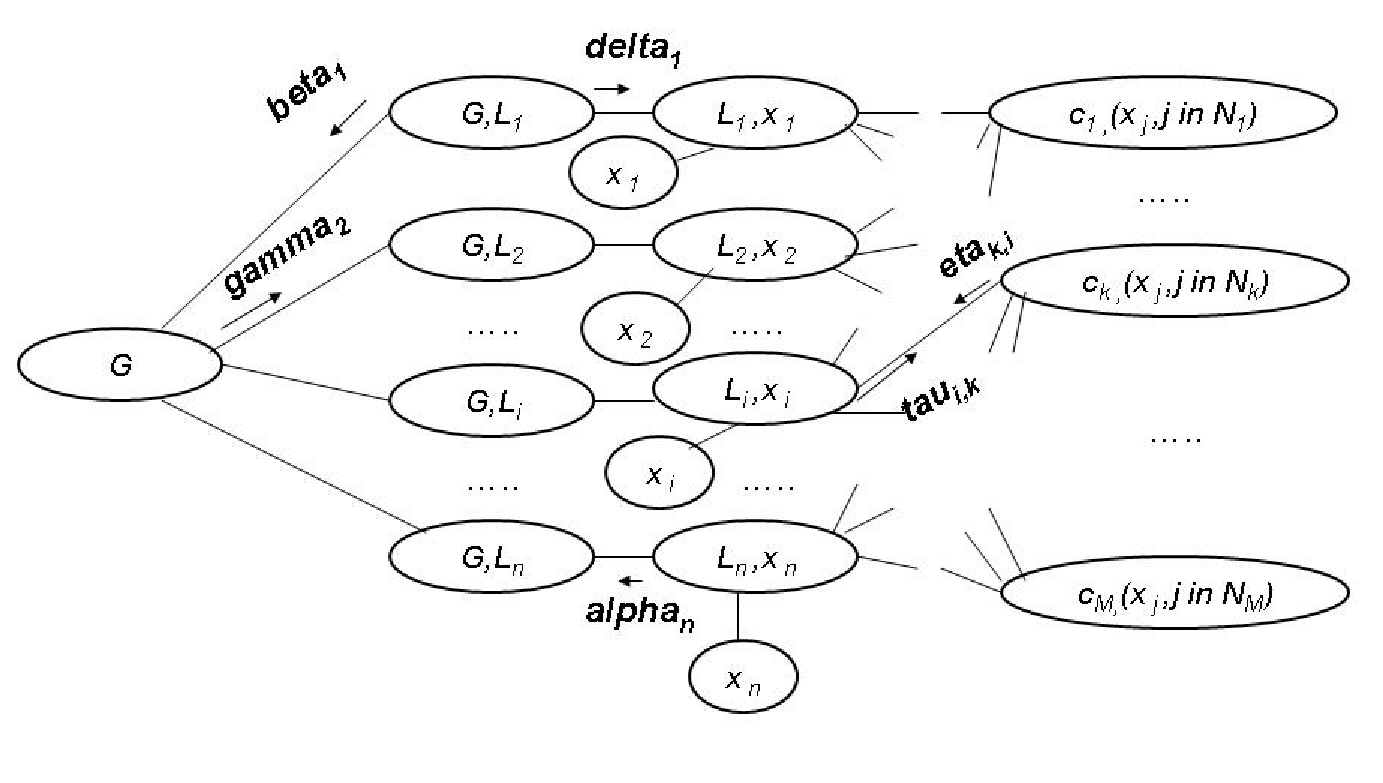
\includegraphics[width=3.0in,height=1.9in]{fig7.eps}
\caption{Junction graph for Step 3.}
\end{figure}

Observe that
\begin{equation}\begin{array}{lll}
P(x_1^n,L_1^n,G|\mathbf{y}_1^{n+s}) \propto \\\varphi(G) \prod_{i}
\varphi(G,L_i) \prod_{i} \varphi(L_i,x_i) \prod_i\varphi(x_i)
\prod_k \varphi(c_k,(x_j, j \in \mathcal{N}_k)).\end{array}
\end{equation}

We may use a message passing algorithm as in \cite{aji} to try to
evaluate  $P(x_i|\mathbf{y}_1^{n+s})$.

Let all messages be initialized to 1, and let $\alpha_j(L_j)$ be
the message sent from $\{L_j,x_j\}$ to $\{G,L_j\}$ at some stage.

The message $\beta_j(G)$ from $\{G,L_j\}$ to $\{G\}$ is then
$\beta_j(G)=\sum_{L_j}\varphi (G,L_j)\alpha_j(L_j)$, and the
message $\gamma_i(G)$ sent from $\{G\}$ to $\{G,L_i\}$ is
$\prod_{j \in \{1,n\}\backslash i} \beta_j(G)$. Finally, the
message from $\{G,L_i\}$ to $\{L_i,x_i\}$ is
$\delta_i(L_i)=\sum_G\varphi(G,L_i)\gamma_i(G)$.

The message $\tau_{j,k}(x_j)$ sent from $\{L_j,x_j\}$ to $\{c_k
(x_j, j \in \mathcal{N}_k)\}$ is $\sum_{L_j}\varphi(L_j,x_j)
\delta_j(L_j)\prod_{l \in \mathcal{N}_j \backslash k}
\eta_{l,j}(x_j)$, where $\eta_{l,j}(x_j)$ is the message from
$\{c_l,(x_j, j\in \mathcal{N}_l)\}$ to $\{L_j,x_j\}$ and is
$\sum_{x_i,i\in \mathcal{N}_l\backslash j}\varphi(c_l, (x_i, i \in
\mathcal{N}_l)) \prod \tau_{i,l}(x_i).$

The message $\alpha_j(L_j)$ is updated to $\sum_{x_j}
\varphi(L_j,x_j) \prod_{k \in \mathcal{N}_j}\eta_{k,j}(x_j)$, and
message exchange continues as above.

As a result, from (\ref{marg}) one gets \begin{equation}P(x_i|
\mathbf{y}_1^{n+s}) \approx
\sum_{L_i}\varphi(L_i,x_i)\delta_i(L_i)\prod_{k \in \mathcal{N}_i}
\eta_k (x_i),\end{equation} and we also have
\begin{equation}
P(G=\underline{g}|\mathbf{y}_1^{n+s}) \approx \prod_{i=1}^n
\beta_i(\underline{g}).
\end{equation}
Even though there are $O(n)$ computations each involving $O(n)$
variables per global iteration step, computational complexity can
be reduced from $O(n^2)$ to $O(n)$ with appropriate organization
of calculations. In particular, $\delta$'s can be computed
directly from $\alpha$'s. For details please see \cite{tech:07}.


The messages $\tau_{j,k}$ and $\eta_{k,j}$ are analogous to
messages computed in a traditional message passing algorithm on a
bipartite graph, so their complexity is also $O(n)$.

Step (4). Compute $\hat{a}'_k \equiv \sum_{i=L}^{M} \hat{b}_i
\hat{f}_i^k \mod P$ for $1\leq k \leq s$, where $\hat{b}_i$ and
$\hat{f}_i$ are obtained from $\mathbf{\hat{c}}$. If
$\hat{a}'_k+\hat{a}^{''}_k \equiv a_k \mod P$ for $1\leq k \leq s$
declare successful decoding.
\subsection{Simulation results}
To be filled in-in progress.\vspace{0in}
\section{Concluding remarks}
We proposed a technique for modifying additive error correction
codes when varying sampling rate causes repetition of symbols. We
presented an encoding scheme which relies on introducing a
carefully chosen prefix such that the overall string (consisting
od the prefix and the codeword) is immune to repetition errors.
The prefix length is only logarithmic in the codeword length. We
also gave a companion message passing algorithm suitable for
decoding of LDPC codes under multiple repetitions and with such a
prefix.

\section*{Acknowledgment}
% optional entry into table of contents (if used)
%\addcontentsline{toc}{section}{Acknowledgment}
The authors would like to thank Marvell Semiconductor Inc. and
U.C. MICRO program for supporting their research.

\begin{thebibliography}{10}
\bibitem{aji}
S. Aji and R. McEliece, ``The generalized distributive law",
\emph{IEEE Trans.  Inform. Theory} vol.\ 46(2), pp.~325--43, March
2000.
\bibitem{apostol} T. M. Apostol, ``\emph{Introduction to Analytic Number
Theory}'', Springer-Verlag, NY, 1976.
\bibitem{cmnv:03}
G. Chen, M. Mitzenmacher, C. Ng and N. Varnica,``Concatenated
codes for deletion channels,'' In \emph{Proc. of the IEEE
International Symposium on Information Theory} 2003, Yokohama,
Japan, p.~218.
\bibitem{dmackay:01}
M.C. Davey and D.J.C. MacKay, ``Reliable communication over
channels with insertions, deletions and substitutions,''
\emph{IEEE Trans. on Information Theory} vol.\ 47(2), pp.~687-698,
Feb. 2001.
\bibitem{isit06} L. Dolecek and V. Anantharam, ''A synchonization
technique for array-based LDPC codes'', \emph{Int. Symp. on
Information Theory}, Seattle, WA, 2006.
\bibitem{tech:07} L. Dolecek and V. Anantharam, ``On reliable communication over channels
with varying sampling rate,'' available at
www.eecs.berkeley.edu/\~{}dolecek/papers
\bibitem{ferr:97}
H.C. Ferreira, W.A. Clarke, A.S.J. Helberg, K.A.S. Abdel-Ghaffar
and A.J. Han Vinck, ``Insertion/deletion correction with spectral
nulls,'' \emph{IEEE Trans. on Information Theory} vol.\ 43(2),
pp.~722--732, March 1997.
\bibitem{huavan:49}
L. K. Hua and H. S. Vandiver, ``Characters over certain types of
rings with applications to the theory of equations in a finite
field'', \emph{Proc. Nat. Acad. Sci. USA}, vol. 35, pp.~481-487,
1949.
\bibitem{lev:66}
V. I. Levenshtein,``Binary codes capable of correcting deletions,
insertions and reversals,'' \emph{Sov. Phys.-Dokl.}, vol.\ 10(8),
pp.~707--710, Feb. 1966.
\bibitem{lev:92}
V. I. Levenshtein, ``On perfect codes in deletion and insertion
metric,'' \emph{Discrete Math. Appl.}, vol.\ 2(3), pp.~241--258,
1992.
\bibitem{liu:02}
J. Liu, H. Song and B.V.K.V. Kumar, ``Symbol timing recovery for
low-SNR partial response recording channels," In \emph{Proc.
GLOBECOM 2003}, Nov. 2002, pp. 1141 -- 1145, San Francisco, CA,
USA.
\bibitem{kbek:04}
P. Kovintavewat, J. R. Barry, M. F. Erden and E. Kurtas,
``Per-survivor timing recovery for uncoded partial response
channels,''\emph{Proceedings of the IEEE International Conference
on Communications} 2004, Paris, France.
\bibitem{sloane:00}
N.J.A. Sloane, ``On single deletion correcting codes,'' 2000.
Available at http://www.research.att.com/\~{ }njas/doc/dijen.pdf
\bibitem{weil:49}
A. Weil, ''Numbers of solutions of equations in finite fields", in
\emph{Bull. Amer. Math. Soc}, vol. 50, pp.~497--508, 1949.
\end{thebibliography}
%\end{document}

%\section{Conclusion}
\label{sec:conclusion}
And thus, we conclude.
%\section{Introduction} 
\label{sec:intro} 
Although distributed programming has become an essential and commonplace task,
it remains very challenging for most developers to write correct distributed
programs. The inherent difficulties of distributed computing---concurrency,
asynchrony, and partial failure---are exacerbated by the scale at which modern
distributed systems operate.

% remind reviewers that it's a database problem. can remove if accepted! 
Much of the discussion about distributed programming today revolves around data
management systems, and the tradeoffs between transactions and loose
consistency. Programmers using distributed transactions are relieved of
consistency concerns but often face significant performance and operational
challenges~\cite{Birman2009}. By contrast, programmers who use loosely
consistent systems can expect more predictable and low-latency performance, but
must reason explicitly about program correctness over inconsistent distributed
state.

In recent years there has been increased interest in techniques to help
programmers achieve correct program behavior without requiring strongly
consistent storage. This idea has been explored in two different frameworks,
\emph{Convergent Objects} and \emph{Monotonic Logic}.

\vspace{0.5em}\noindent
\textbf{Convergent Objects}: In this approach, a programmer writes encapsulated
object classes whose public methods guarantee certain properties regarding
message reordering and/or retry. For example, Statebox is an open-source library
that merges conflicting updates to data items in a key-value store; the user of
the library need only register commutative, idempotent merge
functions~\cite{statebox}. This approach has roots in research in
databases~\cite{Farrag1989,Garcia-Molina1983,Helland2009} and
groupware~\cite{Ellis1989,Sun1998}.  Shapiro et al.\ recently proposed a model
for these approaches called \emph{Conflict-Free Replicated Data Types} (CRDTs),
which formalizes these ideas in an algebraic framework~\cite{Shapiro2011b}.

The main problem with the CRDT approach is that its guarantees of correctness
are limited to an individual replicated data value, not to application logic in
general. For example, consider a distributed algorithmic trading service that
uses a CRDT to represent a mutable set \texttt{Portfolio}. Suppose one server
$M$ reads a local version of the set containing an element \texttt{BNNA} and
constructs an expected portfolio value $v = f(\mbox{\texttt{Portfolio}})$
derived from that version. Concurrently, \texttt{BNNA} is removed from the local
version of \texttt{Portfolio} at another server $N$. The CRDT can ensure that
$M$ and $N$ will eventually agree that \texttt{BNNA} is absent from the set, but
the application state at $M$ and $N$ may remain inconsistent unless the value
$v$ at $M$ is updated to reflect the removal of \texttt{BNNA}. Although the CRDT
maintains its own invariants, the programmer still bears the burden of ensuring
the consistency semantics of the entire program.

\vspace{0.5em} \noindent
\textbf{Monotonic Logic}: In recent work, we observed that the database theory
literature on non-monotonic logic provides a promising starting point for
reasoning about distributed consistency. Intuitively, a \emph{monotonic} program
computes more information over time---it never ``retracts'' an earlier
conclusion in the face of new information. We proposed the CALM
theorem~\cite{Hellerstein2010}, which established that all monotonic programs
are eventually consistent~\cite{Ameloot2011,dedalus-pods12-tr}. Monotonicity of
a Datalog-style program is straightforward to determine conservatively from
syntax, so the CALM theorem provides the basis for a simple analysis technique
for verifying the consistency of distributed programs~\cite{Alvaro2011}. We
realized the CALM analysis as part of Bloom, a Datalog-based DSL for distributed
programming~\cite{bloom}.

The original formulation of Bloom and CALM only validated consistency for programs that compute sets of facts that grow over time (``set monotonicity''); that is, ``growth'' is defined according to set containment. As a practical matter, this is overly conservative: several common distributed programming idioms that are monotonic do not satisfy syntactic monotonicity tests for Datalog. In particular, threshold tests over monotonic aggregate values (e.g., ``$\mathrm{max}(S) > k$'') and upward-moving mutable counters are both considered to be non-monotonic by the original CALM analysis.  As a result, the initial Bloom prototype advises the programmer to guard those constructs with strong consistency methods like Paxos~\cite{Lamport1998} or Two-Phase Commit. 

\subsection{A Hybrid Approach}
% The strengths and weaknesses of these two approaches appear complementary. CRDTs provide synchronization-free consistent objects, but cannot guarantee whole-program consistency. Bloom's CALM analysis guarantees whole-program consistency but is unable to verify a number of natural coordination-free mechanisms.
In this paper, we extend our previous work to accommodate the ideas underlying CRDTs. Instead of only allowing growth according to the set containment
partial order, we allow any user-defined partial order to be used.  
We do this by providing \emph{join semi-lattices} as a programming construct.
We give a
formal definition of this construct below, but the intuition is that the programmer provides a commutative, idempotent merge function (``least upper bound'')
that takes two input values and produces an output value that is not smaller
than either of the input values (according to the user's partial order). This
generalizes Bloom (and traditional Datalog), which assumes a fixed merge
function (set union) and partial order (set containment).
% Relate user-defined merge functions to merge functions in other contexts?
% (e.g., key-value store, COPS, Piccolo)

% Explain how lattices generalize monotonic datalog
It is attractive to incorporate join semi-lattices into logic programming,  but doing so raises challenges in language design, consistency analysis and efficient execution.  In this paper, we make the following contributions:
\begin{enumerate}
% \item
%   We present \baselang, a variant of Datalog that is defined over lattices. We
%   define a model-theoretic semantics for \baselang, and show that \baselang
%   generalizes Datalog.

\item
  We introduce \lang, an extension of Bloom that supports lattices. We detail
  the builtin lattice types provided by \lang and show how developers can
  define new lattices.
  
\item 
  We provide interfaces for consistency-preserving mappings across lattices via
  \emph{morphisms} and \emph{monotonic functions}.  This is critical for \lang
  and forms a useful extension to the CRDT framework as well.

\item 
  We generalize the CALM analysis to programs that contain both lattices and
  set-oriented collections, and show how lattices can be used to prove the
  confluence of several common distributed design patterns that were regarded as
  non-monotonic in Bloom. % XXX: revisit this

\item
  For efficient execution, we show how to extend the standard Datalog semi-naive
  evaluation scheme~\cite{Balbin1987} to support both lattices and traditional
  database relations. We also describe how an existing Datalog engine can be
  extended to support lattices with relatively minor changes.

\item
  Finally, we demonstrate the usefulness of lattices with two case studies.
  First we revisit the simple e-commerce scenario presented in Alvaro et al., in
  which clients interact with a replicated shopping cart
  service~\cite{Alvaro2011}. We show how \lang can be used to make the
  ``checkout'' operation monotonic, despite the fact that it requires
  aggregating over a distributed data set.

  Second, we use \lang to implement vector clocks and causal delivery, two
  standard building blocks for distributed programming. We show how both
  algorithms can be realized as monotonic \lang programs that are concise and
  readable.
\end{enumerate}

\setcounter{page}{1}
\renewcommand{\thepage}{\arabic{page}}\chapter[Dissertation Overview]{Dissertation Overview}
\label{ch:overview}

There has been renewed interest in recent years on applying declarative
languages to a variety of applications outside the traditional boundaries of
data management.  Examples include work on compilers~\cite{lam05context},
computer games~\cite{white-sigmod07}, security protocols~\cite{li-padl03}, and
modular robotics~\cite{ashley-iros07}.  Our work in this area began with the
{\em Declarative Networking} project, as instantiated in the {\em P2} system
for Internet overlays~\cite{p2:sosp, loo-sigmod06}.  This thesis represents the
final chapter of the P2 project and introduces a new exploration of {\em
declarative systems} in the context of {\em cloud
computing}~\cite{abovetheclouds}.

%A number of complex issues arise at the distributed layer, such as resource
%scheduling, the enforcement of distributed invariants (e.g., safety and
%liveness), consistency, availability, and fault-tolerance.  In this thesis, we
%focus on resource scheduling, and how it can be expressed compactly via a
%high-level declarative query language.  We also touch on an initial
%investigation of fault-tolerance in the context of MapReduce, which is another
%high-level dataflow language designed for the {\em
%cloud}~\cite{abovetheclouds}.

Our goal here is to explore systems programming in a high level declarative
language.  This effort is rooted in the {\em Declarative Networking}
project~\cite{boon-thesis}, which ignited the research direction of using a
declarative language to develop distributed software, specifically network
layer protocols and overlays for the next generation of Internet architectures.
In Chapter~\ref{ch:p2}, we review this influential work because it sets the
stage for this thesis.  Specifically, the declarative language \OVERLOG, which
I helped develop during this era, and continued to use throughout my work.  The
\OVERLOG language was accompanied by a runtime called P2, which automatically
compiled \OVERLOG programs into a dataflow-oriented runtime system.

The primary contributions presented in this dissertation begin in
Chapter~\ref{ch:evita}, where we describe our first declarative system
component -- Evita Raced, which is a declarative metacompiler implemented in
the final version of P2.  Evita Raced formulates the task of query compilation
as a query; written in the same declarative language (\OVERLOG) used by
``client'' queries, such as the various networking protocols from Loo, et
al.~\cite{loo-sigmod06, p2:sosp}.  The P2 compiler was first engineered to
compile query code into a relational format, thereby providing compilation
tasks (written in \OVERLOG) access to the logical query plan, and allowing the
ability to query and update that logical query plan.  We show that many
traditional database optimizations, like the magic-sets rewrite
(Chapter~\ref{ch:magic}), the System R dynamic program
(Chapter~\ref{ch:opt:sec:systemr}), and the Cascades branch-and-bound algorithm
(Chapter~\ref{ch:opt:sec:cascades}), can be fully expressed as \OVERLOG
queries.  Specifying these optimizations as \OVERLOG queries resulted in a more
concise representation of the {\em algorithm} as {\em code} and a dramatic
reduction in the overall development effort.  However, the pragmatics of
operating in a distributed environment led to a number of hacks that sacrificed
declarativity.  We reflect on the practicalities of system development and our
overall experience with Evita Raced in Chapter~\ref{ch:evitaend}.
 
In Chapter~\ref{ch:cloud}, we turn our attention to another system that has
gained in popularity recently --- Apache Hadoop~\cite{hadoop}.  Hadoop is an
open source software project that implements the MapReduce programming
model~\cite{mapreduce-osdi}.  In our work here, we investigated the Hadoop task
scheduling component, which is housed within the centralized coordinator of the
Hadoop MapReduce engine.  It is written in the (relatively) low-level Java
language~\cite{java}.  As we have already suggested, building and debugging
distributed software can be extremely difficult in such a procedural language.  We
conjecture that by adopting a {\em data-centric} approach to system design and
by employing {\em declarative} programming languages, a broad range of
distributed software functionality can be recast naturally in a data-parallel
programming model.  Our hope is that this model can significantly raise the
level of abstraction for programmers, improving code simplicity, speed of
development, ease of software evolution, and program correctness.

To evaluate this conjecture, we used the \OVERLOG language to implement an
API-compatible version of the Hadoop MapReduce scheduler.  Not only did we
achieve this goal using {\em orders of magnitude} fewer lines of code, our
implementation exhibits competitive performance, and extends Hadoop with
advanced fault-tolerance and scaling features that are typical for cloud
computing environments.  In Chapter~\ref{ch:hadoop}, we provide some background
material on MapReduce, which has emerged as a popular programming model for
writing data processing tasks in the cloud.  In Chapter~\ref{ch:boom}, we describe
our rewrite of the Hadoop MapReduce scheduling engine in a declarative language
and show that equivalent performance, fault-tolerance, and scalability
properties can be achieved in orders-of-magnitude less code.  In
Chapter~\ref{ch:hop}, we move beyond the batch-oriented execution model in
MapReduce to a more online execution model by pipelining data between system
operators.  This extension brings with it a number of scheduling challenges,
which we resolve in our declarative scheduling framework.  Finally, we conclude
in Chapter~\ref{ch:conclusion} with a discussion of future directions.





\part[Communication Over Channels With Varying Sampling Rate]{Communication Over Channels With Varying Sampling Rate}
\chapter[Introduction]{Introduction}\label{intro1}

In a typical communication system a binary input message
$\mathbf{x}$ is encoded at the transmitter, using a
substitution-error correcting code $C$, into a coded sequence
$\mathbf{c}$ = $C(\mathbf{x})$, which we will assume is also a
binary sequence. The modulated version of this sequence may be
modeled as being corrupted by additive noise, so the received
waveform after matched filtering  can be written as
\begin{equation}
r(t)=\sum_{i} c_i h(t-iT) +n(t),
\end{equation}
where $c_i$ is the $i^{th}$%$i^{\text{th}}$
bit of $\mathbf{c}$, $h(t)$ is convolution of the modulating pulse
and the matched filter, and $n(t)$ represents the noise introduced
by the channel.

The receiver samples $r(t)$ at time instances
$\left\{kT_s+\tau_k\right\} $, and the sequence of samples is fed
into the decoder which decides on the most likely input message.
Accurate synchronization of the sampling instants, i.e that $T_s$
be equal to $T$ and that each $\tau_k$ be ideal, is critical for
the full utilization of the coding gain of the substitution-error
correcting code. As the operating requirements under which timing
recovery must be performed become more stringent, because of
higher data rates and/or longer delays in the decision feedback
loop that adjusts the sampling instants, such synchronization is
becoming harder to achieve. Several authors have studied the
problem of accurate timing recovery. Proposed solutions include
building a more sophisticated timing recovery block \cite{liu:02},
multiple hypothesis analysis of the sampling instances
\cite{kbek:04}, and for the intersymbol interference (ISI)
channels in particular, a soft-output detector for both ISI and
timing errors \cite{zhangkavcic:03}, and an iterative timing
recovery approach that incorporates timing recovery in turbo
equalization \cite{iterativetr:04}.

As an alternative to more complex and more expensive timing recovery
schemes, we propose to shift the emphasis away from the timing
recovery block  and instead modify the decoding procedure and the
code itself to compensate for inadequate synchronization. By
analyzing the robustness of a substitution-error correction code to
synchronization errors, one could use a subcode of the original code
that would have good minimum distance under both substitution as
well as sampling errors. The trade-off would be between the incurred
rate loss associated with the code modification versus the increased
complexity and latency associated with the existing approaches
mentioned above. The challenge of the proposed approach lies in
determining the synchronization error correction capabilities of
individual codes of interest, and in determining as large as
possible a subcode with the desired properties.  The proposed
approach can be considered for any system, and it is especially
relevant for practical pilotless communication systems.


To illustrate the issues that arise when adequate timing recovery
is missing, assume (for purposes of argument) that $h(t)$ is a
rectangular pulse of duration $T$ and unit amplitude and that we
are operating in the infinite signal-to-noise (SNR) regime where
the effect of $n(t)$ is negligible. Then $r(t)$ simply becomes
\begin{equation}
r(t)= \sum_{i} c_i 1(iT\leq t < (i+1)T)~.
\end{equation}

If samples were taken in the middle of each pulse the sampled
version of $r(t)$ would be precisely $\mathbf{c}$. Now suppose
that inadequate timing recovery causes the sampling to occur at
time instants $kT_s+\tau_k$.
\begin{figure}\label{figa}
\begin{picture}(50,100)(0,40)
\put(10,50){\vector(1,0){220}} \put(10,50){\vector(0,1){70}}
\put(50,50){\line(0,1){50}} \put(90,50){\line(0,1){50}}
\put(130,50){\line(0,1){50}} \put(170,50){\line(0,1){50}}
\put(210,50){\line(0,1){50}} \put(50,100){\line(1,0){40}}
\put(130,100){\line(1,0){40}} \put(170,100){\line(1,0){40}}
\put(0,100){{1}} \put(0, 130){{$r(t)$}} \put(30,30){{T}}
\put(70,30){{2T}}\put(110,30){{3T}}\put(150,30){{4T}}
\put(190,30){{5T}} \put(220, 70){{$\ldots$}} \put(235,40){{$t$}}
\put(50,100){\line(1,0){5}} \put(27,47){{$\diamond$}}
\put(62,97){{$\diamond$}} \put(97,47){{$\diamond$}}
\put(132,97){{$\diamond$}} \put(162,97){{$\diamond$}}
\put(200,97){{$\diamond$}} \put(30,47){\line(0,1){5}}
\put(70,47){\line(0,1){5}} \put(110,47){\line(0,1){5}}
\put(150,47){\line(0,1){5}}\put(190,47){\line(0,1){5}}
\put(10,100){\line(1,0){5}}
\end{picture}

\caption{An example of oversampling.}\label{pic:graph2}
\end{figure}

As an example, consider a sequence $\mathbf{c}$ =
(0,1,0,1,1,$\ldots$) that results in the waveform $r(t)$ shown in
Figure~\ref{figa}. The sampling points $kT_s+\tau_k$ are marked in
the figure by $\diamond$. In this example, $T_s<T$ causes
oversampling, and the sampled version of $r(t)$ contains a
repeated bit (here the fourth bit is sampled twice).
%\input{figure2.tex}
Analogously, when $T_s>T$, undersampling can cause the separation
between two consecutive samples to be so large that some bit is
not sampled at all. Therefore without adequate timing recovery the
sampled version of $r(t)$ results in a sequence obtained by
repeating or deleting some bits in $\mathbf{c}$.


In this work we adopt a set-theoretic model for the synchronization
errors in which a codeword gives rise to a set of possible received
sampled sequences which depends on how many bits are allowed to be
repeated or deleted. A codeword $\mathbf{c}$ can in general give
rise to a whole set of received sampled versions of $r(t)$. The
possible set of such sequences depends on how good the timing
recovery scheme is. When two distinct codewords $\mathbf{c_1}$ and
$\mathbf{c_2}$ can result in the same sampled sequence, it is no
longer possible to uniquely determine the coded sequence or its
pre-image $\mathbf{x}$ from the received sequence, even in the
noise-free environment. We then say that the substitution-error
correcting code $C$ has an \textit{identification problem}. We also
say that the pair of codewords $\mathbf{c_1}$ and $\mathbf{c_2}$ has
an identification problem.

More generally, two distinct codewords $\mathbf{c_1}$ and
$\mathbf{c_2}$ could result in sampled sequences with poor Hamming
distance. This would result in poor performance over a channel
that permits substitution errors. In this case we say that the
substitution-error correcting code $C$ has {\em poor
identification}. We also say that the pair of codewords
$\mathbf{c_1}$ and $\mathbf{c_2}$ has poor identification.




It should be mentioned that several authors have studied codes
immune to insertions and deletions of bits. For example, the
so-called Varshamov-Tenengolts code proposed in \cite{vt:65} and
popularized by Levenshtein in \cite {lev:66} has been further
studied by Ferreira et al., \cite {ferr:97}, Levenshtein
\cite{lev:92}, Sloane \cite{sloane:00}, and Tenengolts
\cite{ten:84}. Related constructions were proposed in
\cite{bours:94}, \cite{calabi:69}, \cite{clarke:93}, \cite{klove:95}
and \cite{ullman:66}. Even though these constructions result in
codes that are immune to a given number of insertions and deletions
of bits, they have a limited guarantee for other desirable
properties of standard substitution-error correcting codes (such as
linearity and a good minimum Hamming distance). Several other
authors have proposed concatenated codes that correct
synchronization errors, such as in \cite{cmnv:03}, \cite{cf:03}, and
\cite{dmackay:01}. In contrast to these works, our approach is to
start with known substitution-error correcting codes and propose
ways to modify them with only a small loss in the rate in order to
continue to provide good performance under synchronization errors,
which are themselves modeled as a certain number of repetitions or
deletions of bits. A related problem of a code construction for
frame synchronization was studied in \cite{stiffler:65} and
\cite{bose:67}.


The next two Chapters focus on the analysis of the first order
Reed-Muller codes under the synchronization and substitution errors.
We first prove several new structural properties of these codes in
Chapter~\ref{reed-muller-struc}, which are then subsequently used in
Chapter~\ref{reed-muller-perfm} where we discuss how to
systematically thin these codes to improve their performance under
synchronization and substitution errors, and how to efficiently
decode thinned codes when both types of errors are present.
Chapter~\ref{numbertheory} discusses explicit number-theoretic
constructions of sets of strings capable of overcoming repetition
errors. The focus of this chapter is on deriving cardinality results
of these constructions using combinatorial and number-theoretic
methods. Lastly, Chapter~\ref{prefixing} discusses how to improve
repetition error correcting capability of a collection of binary
strings  by judiciously appending a prefix to a string belonging to
this collection  using the number-theoretic construction from
Chapter~\ref{numbertheory}.

%\documentclass[journal]{IEEEtran}
%\documentclass[12pt]{article}
%\pagestyle{plain} \topmargin -0.60in \oddsidemargin 0.0625in
%\textheight 9.00in \textwidth 6.50in
%\renewcommand{\baselinestretch}{1.4}
%\parskip 0.20in

%\usepackage{times}
%\usepackage{psfig,latexsym}
%\usepackage{amstext,amssymb}
%\newtheorem{corollary}{Corollary}[section]
%\newtheorem{theorem}{Theorem}[section]
%\newtheorem{lemma}{Lemma}[section]
%\newtheorem{definition}{Definition}[section]
%\newtheorem{fact}{Fact}
%\newtheorem{remark}{Remark}[section]
%\newcommand{\x} {\mbox{x}}
%\newenvironment{proof}%
 %              {\par\noindent%
  %             \setlength{\parindent}{0em}%
   %            \setlength{\parskip}{1ex}%
    %           \textit{Proof:\nopagebreak[2]
%}}{\hfill\rule{1.5ex}{1.5ex}\par}
\newcommand{\revc}{{{\stackrel{c}{\leftarrow}}}}
\newcommand{\revca}{{{\stackrel{\mathbf{c_a}}{\leftarrow}}}}
\newcommand{\revcb}{{{\stackrel{\mathbf{c_b}}{\leftarrow}}}}
\newcommand {\bb}{\mathbf}
\newcommand{\tr}{\text{tr}}
\newcommand {\bt}[1]{\mathbf{\tilde{#1}}}
\newcommand {\bh}[1]{\mathbf{\hat{#1}}}
\newcommand{\blist}{    \begin{list}{$\bullet$}{\topsep 0.0in \partopsep
0.0in                \itemsep 0.05in \parsep
           0.0in \leftmargin 0.3in}}


\newcommand{\elist}{\end{list}}
%\pagenumbering{arabic}

%\documentclass[journal, twocolumn]{IEEEtran}


%\usepackage{amsmath}   % From the American Mathematical Society
                        % A popular package that provides many helpful commands
                        % for dealing with mathematics. Note that the AMSmath
                        % package sets \interdisplaylinepenalty to 10000 thus
                        % preventing page breaks from occurring within multiline

%\usepackage{times}
%\usepackage{psfig,latexsym}
%\usepackage{amstext,amssymb}
%\usepackage{amstext,amssymb}



% correct bad hyphenation here
\hyphenation{op-tical net-works semi-conduc-tor}


%\setlength{\textheight}{11.85cm}

%\begin{document}
%
% paper title
\chapter[Structural Properties of Reed-Muller Codes]{Structural Properties of Reed-Muller
Codes}\label{reed-muller-struc} In this Chapter we establish
several new structural properties of the first order Reed-Muller
codes. These properties, while also of independent interest, will
be used in the subsequent chapter that discusses the performance
of Reed-Muller codes under synchronization and substitution
errors. Having provided a definition of the first order
Reed-Muller codes in Section \ref{sectionRM1}, we prove several
runlength properties of these codes in Section \ref{sectionRM2}.
In particular, we establish several properties regarding the
runlength distribution (Subsection \ref{sectionRM21}), runs of
runs of codewords (Subsection \ref{sectionRM22}), as well as the
relationship between the message vector and the runs of its
codeword (Subsection \ref{sectionRM23}). Section
\ref{sectionRMconc} concludes this Chapter.


%% compare with version 1

%\begin{keywords} Synchronization, repetitions and deletions,
%Reed-Muller code, run-length properties.
%\end{keywords}

% Note that keywords are not normally used for peerreview papers.

% For peer review papers, you can put extra information on the cover
% page as needed:
% \begin{center} \bfseries EDICS Category: 3-BBND \end{center}
%
% For peerreview papers, inserts a page break and creates the second title.
% Will be ignored for other modes.
%% compare with version 1
%%\IEEEpeerreviewmaketitle




\section{First Order Reed-Muller Codes}\label{sectionRM1}
The first order Reed-Muller codes RM($1$,$m$) are linear $(2^m,
m+1)$ substitution-error correcting codes \cite{mws:77}. They have
good minimum distance, equal to $2^{m-1}$, simple encoding, and a
relatively low complexity maximum likelihood decoding algorithm
($O(n \log n)$ for $n=2^m$). On the negative side, they have low
rate.

From now on, let $C(m)$ denote the RM($1$,$m$) code. The code
$C(m)$ may be described by an $(m+1) \times 2^m$ generator matrix
$\mathbf{G_m}$ given by
\begin{equation*}\label{eq:g}
 \begin{array}{lll} \mathbf{G_m} &=
\left[ \begin{array}{c} \underline{1} \\ \mathbf{M_m} \end{array} \right] \\
{} & {}\\
{} &=\left[ \begin{array}{cccccccccc}
1 & 1 & 1 & 1 & 1 & \ldots & 1 & 1 & 1 & 1 \\
1 & 1 & 1 & 1 & 1 & \ldots & 0 & 0 & 0 & 0 \\
\ldots & \ldots & \ldots & \ldots &\ldots &\ldots & \ldots & \ldots & \ldots &\ldots\\
1 & 1 & 1 & 1 & 0 & \ldots & 0 & 0 & 0 & 0 \\
1 & 1 & 0 & 0 & 1 & \ldots & 1 & 1 & 0 & 0 \\
1 & 0 & 1 & 0 & 1 & \ldots & 1 & 0 & 1 & 0\\
\end{array}\right],
\end{array}
\end{equation*}

\noindent were $\underline{1}$ denotes the binary string of length
$2^m$ with all entries equal to 1, and the $m$ by $2^m$ submatrix
$\mathbf{M_m}$ consists of lexicographically decreasing binary
columns of length $m$. Observe that the $i^{\text{th}}$ row of
$\mathbf{G_m}$, for $1 <i \leq m+1$, consists of $2^{i-1}$
alternating runs of ones and zeros, and that each run is of length
$2^{m-i+1}$.

 For future
reference, we recall that every codeword in $C(m+1)$ is either the
concatenation of a codeword in $C(m)$ with itself or the
concatenation of a codeword in $C(m)$ with its bitwise complement
\cite[Thm. 2, pg. 374]{mws:77}. The concatenation of two binary
strings $a$ and $b$ will be written as $[a | b]$. If $c$ is a
codeword in $C(m)$ it is straightforward to check that its bitwise
complement, denoted $\overline{c}$, is also a codeword in $C(m)$.
Further, its reversal, i.e. the binary string got by reading $c$
from its end to its beginning, denoted $\revc$, is also a codeword
in $C(m)$. Since the operations of bitwise complementation and
reversal commute, we may unambiguously denote the complement of
the reversal of $c$ as $\overline{\revc}$.

We now establish several runlength properties of Reed-Muller
codes.

\section{Runlength Properties of the RM($1$,$m$)
Codes}\label{sectionRM2}

\subsection{Run-length distribution}\label{sectionRM21}
\begin{lemma}\label{Lem1}
The codewords in $C(m)$ can
be partitioned into $2^{m-1}+1$ distinct
non-empty groups $G_j^m$,
for $0 \leq j \leq 2^{m-1}$.
Here $G_j^m$ is comprised of
those codewords in $C(m)$ that have
$j$ runs of ones.
$G_0^m$ is comprised of
exactly one codeword, namely the all-zero codeword. This codeword will be denoted
$c_0^m(00)$.
There are 4 distinct codewords in each
group $G_j^m$, for $1 \le j  < 2^{m-1}$.
These codewords may be uniquely identified
by their first and last bit. They may
thus be unambiguously denoted as
$c_j^m(11)$, $c_j^m(10)$, $c_j^m(01)$,
and  $c_j^m(00)$ respectively.
There are 3 distinct
codewords in the group $G_{2^{m-1}}^m$.
These codewords may also be uniquely identified
by their first and last bit and may
be unambiguously denoted as
$c_{2^{m-1}}^m(11)$,
$c_{2^{m-1}}^m(10)$,
and  $c_{2^{m-1}}^m(01)$ respectively.
\end{lemma}

\noindent \textit{Proof:} The proof is by induction on $m$. For
$m=1$ and $m=2$ the statement can be verified by inspection.
Suppose the assertion holds for all $1 \le m \le m_0$.

Let us first consider the group $G_j^{m_0}$ for $1 \leq j <
2^{m_0-1}$. By assumption, it contains 4 codewords, unambiguously denoted
as  $c_j^{m_0}(11)$,
$c_j^{m_0}(01)$, $c_j^{m_0}(10)$, and $c_j^{m_0}(00)$ respectively.
Out of the eight possible concatenations of each such codeword with either itself or its complement, 3 result in codewords in
$G_{2j-1}^{m_0+1}$ (these are [$c_j^{m_0}(11)|c_j^{m_0}(11)$],
[$c_j^{m_0}(11)|$$\overline{c_j^{m_0}(11)}$], and
[$c_j^{m_0}(01)|$$\overline{c_j^{m_0}(01)}$]), 4 result in codewords
in $G_{2j}^{m_0+1}$ (these are [$c_j^{m_0}(01)|c_j^{m_0}(01)$],
[$c_j^{m_0}(10)|$ $\overline{c_j^{m_0}(10)}$],
[$c_j^{m_0}(10)|c_j^{m_0}(10)$], and
[$c_j^{m_0}(00)|c_j^{m_0}(00)$]), and 1 results in the codeword
[$c_j^{m_0}(00)|$$\overline{c_j^{m_0}(00)}$] in $G_{2j+1}^{m_0+1}$.
By varying $j$ from $1$ to $2^{m_0-1}-1$, inclusive,
we thus describe 3 codewords in $G_1^{m_0+1}$, 4 codewords in each
$G_{j'}^{m_0+1}$ for $ 2 \leq j' \leq 2^{m_0}-2$ and 1 codeword in
$G_{2^{m_0}-1}^{m_0+1}$ such that no two codewords that belong to
the same group $G_{j'}^{m_0+1}$ agree in both the first and the last bit.

Now consider the group $G_{2^{m_0-1}}^{m_0}$. By assumption it has
three codewords unambiguously denoted as
$c_{2^{m_0-1}}^{m_0}(11)$, $c_{2^{m_0-1}}^{m_0}(01)$, and
$c_{2^{m_0 -1}}^{m_0}(10)$ respectively. There are six
possibilities arising from concatenations of such a codeword with
itself or its complement. Of these, 3 result in codewords in
$G_{2^{m_0}-1}^{m_0+1}$ (these are $[c_{2^{m_0 -1}}^{m_0}(01)
|$$\overline {c_{2^{m_0-1}}^{m_0}(01)}]$ $[c_{2^{m_0
-1}}^{m_0}(11) |$$c_{2^{m_0 -1}}^{m_0}(11)]$, and $[c_{2^{m_0
-1}}^{m_0}(11) |$$\overline{c_{2^{m_0 -1}}^{m_0}(11)}]$) and the
remaining 3 result in the codewords of $G_{2^{m_0}}^{m_0+1}$. Note
that none of the latter three concatenations has both outer bits
equal to '0'. Note that we have now described a total of 4
codewords in the group $G_{2^{m_0}-1}^{m_0+1}$, no two agree in
both first and last bit, and we have also described 3 codewords in
the the group $G_{2^{m_0}}^{m_0+1}$ of the desired form.

The concatenation of the all-zero codeword in $C(m_0)$ with the
all-ones codeword yields the fourth codeword in $G_1^{m_0+1}$, and
its concatenation with itself yields the only codeword in $G_0^{m_0+1}$.

We have therefore described $1+4\times(2^{m_0}-1)+3=2^{m_0+2}$
codewords in $C(m_0+1)$, which is precisely the cardinality of
this code, and we showed that the proposed statement holds for
it.\hfill $\blacksquare$

By exploiting the result in Lemma~\ref{Lem1},
it is easy to verify
the following, which may also of course
be seen more directly.

\begin{lemma}\label{LE2}
For each $1 \leq k \leq 2^m$,
in $C(m)$ there are exactly 2 codewords which have a total of $k$
runs, and they are bitwise complements of each
other.
\end{lemma}

\noindent \textit{Proof:} The complementary codewords
$c_{j-1}^m(00)$ and $c_{j}^m(11)$ each have $2j-1$ runs. Letting
$j$ run from $1$ through $2^{m-1}$ gives $2^{m-1}$ such
complementary pairs of codewords. The complementary codewords
$c_j^m(10)$ and $c_j^m(01)$ each have
 $2j$ runs. Letting
$j$ run from $1$ to $2^{m-1}$
gives another
$2^{m-1}$ such complementary pairs
of codewords.
This completes the proof. \hfill $\blacksquare$


\begin{lemma}\label{LE3}
Consider a codeword $\mathbf{c}$ in $C(m)$. Either $\mathbf{c}$
has all its runs of the same length, which is a power of $2$, or
the runs in $\mathbf{c}$ are of two different lengths, and these
two lengths are consecutive powers of 2. In addition, if there are
runs of two different lengths in $\mathbf{c}$, the outer runs
(i.e. the leftmost run and the rightmost run) in $\mathbf{c}$ are
of the smaller length.
\end{lemma}

\noindent \textit{Proof:} The proof is by induction on $m$. It is
straightforward to check the truth of the statement for $m=1$ and
$m=2$. Suppose now that the given statement is true for all $1 \le
m \le m_0$. For a codeword $\mathbf{c}$ in $C(m_0)$ let
$[\mathbf{c} | \mathbf{c}]$ and $[\mathbf{c} |
\mathbf{\overline{c}}]$ denote the codewords in $C(m_0+1)$ that
are the concatenation of $\mathbf{c}$ with itself, and the
concatenation of $\mathbf{c}$ with its complement, respectively.

Suppose first that $\mathbf{c}$ has all its runs of the same
length, equal to $2^s$ for some $s \ge 0$. If $\mathbf{c}$ has the
same starting and ending bits then in the concatenation
$[\mathbf{c} | \mathbf{\overline{c}}]$ all runs have the same
length $2^s$, so the statement of the lemma holds. In the
concatenation $[\mathbf{c} | \mathbf{c}]$ all runs except the run
at the point of concatenation (if there are any such runs) have
length $2^s$ and the run at the point of concatenation has length
$2^{s+1}$. The proposed statement continues to be true both in the
case in which there are some runs other than the one at point of
concatenation and in the case when there are no such runs. If
$\mathbf{c}$ starts and ends with different bits, we may repeat
the previous argument mutatis mutandis.

Now suppose that $\mathbf{c}$ has runs of different lengths, which
are two consecutive powers of 2, say $2^s$ and $2^{s+1}$. By
assumption, the outer runs are of length $2^s$ each, and there is
at least one run of length $2^{s+1}$. As before, if $\mathbf{c}$
starts and ends in the same bit, the concatenation $[\mathbf{c} |
\mathbf{\overline{c}}]$ will have all its runs of lengths either
$2^s$ or $2^{s+1}$. Further, the outer runs in $[\mathbf{c} |
\mathbf{\overline{c}}]$ have the same length as the ones in
$\mathbf{c}$, i.e. they are of length $2^s$ each, so the statement
of the lemma is valid. In the concatenation $[\mathbf{c}
|\mathbf{c}]$, the last run in the left copy of $\mathbf{c}$ and
the first run in the right copy of $\mathbf{c}$ are merged
together, and all other runs are unchanged in length. By
assumption, the outer runs in $\mathbf{c}$ have length $2^s$ each,
so their merger results in a run in $[\mathbf{c} | \mathbf{c}]$ of
length $2 \times 2^s=2^{s+1}$. Thus all runs in $[\mathbf{c} |
\mathbf{c}]$ have length either $2^s$ or $2^{s+1}$. Since the
outer runs in $[\mathbf{c} |\mathbf{c}]$ are of the same length as
the outer runs in $\mathbf{c}$, they have length $2^s$, as
required. For $\mathbf{c}$ starting and ending in different bits,
we repeat this argument mutatis mutandis.

Since each
codeword in $C(m_0+1)$ can be written as a concatenation of a
codeword in $C(m_0)$ either with itself or with its complement,
the proof of the Lemma is complete.\hfill $\blacksquare$

\small
\begin{figure*}{
\begin{picture}(100,150)(30,40)

%\put(255,205){{$c_1^0(11)$='1'}}
%\put(190,205){{$c_0^0(00)$='0'}}


\put(-12,135){$\ldots$}

\put(10,135){{$c_{j-1}^{m_0}(00)$}}
\put(67,135){{$c_{j}^{m_0}(11)$}}
\put(134,135){{$c_j^{m_0}(01)$}}
\put(186,135){{$c_j^{m_0}(10)$}}
\put(265,135){{$c_j^{m_0}(00)$}}
\put(310,135){{$c_{j+1}^{m_0}(11)$}}
\put(356,135){{$c_{j+1}^{m_0}(01)$}}
\put(401,135){{$c_{j+1}^{m_0}(10)$}}
\put(446,135){{$c_{j+1}^{m_0}(00)$}}
\put(485,135){$\ldots$}
%\put(-35,75){{$c_{2j-2}^{m_0+1}(00)$}}
\put(-15,75){$\ldots$}
\put(3,75){{$c_{2j-1}^{m_0+1}(11)$}}
\put(52,75){{$c_{2j-1}^{m_0+1}(01)$}}
\put(100,75){{$c_{2j-1}^{m_0+1}(10)$}}

\put(149,75){{$c_{2j-1}^{m_0+1}(00)$}}
\put(197,75){{$c_{2j}^{m_0+1}(11)$}}
\put(245,75){{$c_{2j}^{m_0+1}(01)$}}
\put(293,75){{$c_{2j}^{m_0+1}(10)$}}

\put(341,75){{$c_{2j}^{m_0+1}(00)$}}
\put(390,75){{$c_{2j+1}^{m_0+1}(11)$}}
\put(438,75){{$c_{2j+1}^{m_0+1}(10)$}}
\put(485,75){$\ldots$}

\put(430,110){$\ldots \ldots \ldots$}
\put(40,100){\text{1}}
\put(108,100){\text{2}}
\put(153,100){\text{3}}
\put(194,100){\text{4}}
\put(222,100){\text{5}}
\put(269,100){\text{6}}
\put(335,100){\text{7}}
\put(412,100){\text{8}}

%\put(425,75){{$c_{2j+1}^{m_0+1}(01)$}}
%\put(471,75){{$c_{2j+1}^{m_0+1}(10)$}}

%\put(517,75){{$c_{2j+1}^{m_0+1}(00)$}}
%\put(563,75){{$c_{2j+2}^{m_0+1}(11)$}}
%\put(436,75){{$c_{2j+2}{m_0+1}(01)$}}
%\put(470,75){{$c_{2j+2}^{m_0+1}(10)$}}
%\put(420,115){{1010}}

%\put(450,110){\vector(3,-2){35}}
%\put(450,110){\vector(-3,-2){35}}
%\put(410,110){\vector(3,-2){35}}
%\put(410,110){\vector(-3,-2){35}}

%\put(320,110){\vector(3,-2){35}}
%\put(320,110){\vector(-3,-2){35}}

\put(335,130){\vector(4,-1){158}}
\put(335,130){\vector(3,-2){68}}
\put(288,130){\vector(4,-1){170}}
\put(288,130){\vector(3,-2){68}}

\put(205,130){\vector(2,-1){92}}
\put(205,130){\vector(1,-2){21}}
\put(160,130){\vector(0,-1){42}}
\put(160,130){\vector(2,-1){90}}

\put(75,130){\vector(1,-1){44}}
\put(75,130){\vector(-1,-1){44}}
\put(25,130){\vector(1,-1){44}}
\put(25,130){\vector(-1,-1){35}}

%\put(2,70){\line(0,-1){20}}
%\put(195,70){\line(0,-1){20}}
%\put(200,70){\line(0,-1){20}}
%\put(385,70){\line(0,-1){20}}
%\put(390,70){\line(0,-1){20}}
\put(2,65){$\underbrace{\hspace{2.65in} } $}
\put(198,65){$\underbrace{\hspace{2.65in} } $}
\put(392,65){$\underbrace{\hspace{1.5in} } $}
\put(100,50){$G_{2j-1}^{m_0+1}$}
\put(300,50){$G_{2j}^{m_0+1}$}
\put(420,50){$G_{2j+1}^{m_0+1}$}

\put(190,155){$G_j^{m_0}$}
\put(28,155){$G_{j-1}^{m_0}$}
\put(398,155){$G_{j+1}^{m_0}$}
\put(-12,145){$\overbrace{\hspace{0.95in} } $}
\put(60,145){$\overbrace{\hspace{3.35in} } $}
\put(305,145){$\overbrace{\hspace{2.4in} } $}
%\put(35,70){\vector(0,-1){30}}
%\put(75,70){\vector(0,-1){30}}
%\put(105,70){\vector(0,-1){30}}

%\put(125,70){\vector(0,-1){30}}
%\put(155,70){\vector(0,-1){30}}
%\put(195,70){\vector(0,-1){30}}
%\put(225,70){\vector(0,-1){30}}

%\put(245,70){\vector(0,-1){30}}
%\put(275,70){\vector(0,-1){30}}
%\put(315,70){\vector(0,-1){30}}
%\put(345,70){\vector(0,-1){30}}

%\put(365,70){\vector(0,-1){30}}
%\put(395,70){\vector(0,-1){30}}
%\put(435,70){\vector(0,-1){30}}
%\put(465,70){\vector(0,-1){30}}
\put(-15,40){\line(1,0){515}} \put(-15,180){\line(1,0){515}}
\put(-15,180){\line(0,-1){140}} \put(500,180){\line(0,-1){140}}
\end{picture}}
 \caption{Construction of codewords in $C(m_0+1)$ from codewords
in $C(m_0)$.}\label{pic:graph1}
\end{figure*}



\normalsize
\begin{lemma}\label{LE4}
With the exception of the all-ones codeword, all codewords
belonging to the group $G_j^m$ for $2^{p-1}<j \leq 2^{p}$ for some
$p$, $0 \leq p \leq m-1$ have all runs of ones either of length
$2^{m-p-1}$ or of length $2^{m-p}$. Moreover, $(j-2^{p-1})\times
2$ runs out of these $j$ runs have length $2^{m-p-1}$, and the
remaining $2^{p}-j$ runs have length $2^{m-p}$.
\end{lemma}
\noindent \textit{Proof:} To prove the statement we use induction
on $m$. For small values of $m$, the proposed statement can be
verified directly. Suppose now that the assertion holds for some
$m=m_0$.

By Lemma~\ref{LE1}, the group $G_{j'}^{m_0}$ for $2^{p-1}< j' \leq
2^{p}$ for some $p$, $0 \leq p \leq m_0-1$ contains codewords
$c_{j'}^{m_0}(10)$, $c_{j'}^{m_0}(01)$, and $c_{j'}^{m_0}(11)$. If
$j' \neq 2^{m_0-1}$ it also contains $c_{j'}^{m_0}(00)$. There is
a single codeword in $G_0^{m_0}$ (the all-zeros codeword). Let us
now analyze all the possible concatenations of the codewords
belonging to the group $G_j^{m_0}, 0 \leq j \leq 2^{m_0-1}$ i.e.
of each codeword with itself and with its complement. By
Lemma~\ref{LE1} there are at most 4 codewords in $G_j^{m_0}$ so we
have to consider at most 8 different concatenations. In doing so,
the similar cases will be presented together.
\begin{itemize}
\item The concatenation of $c_j^{m_0}(11)$, if it exists, with
itself produces a codeword in $G_{2j-1}^{m_0+1}$ (see Arrow 1 in
Figure~\ref{pic:graph1}).

If $j=1$, $c_j^{m_0}(11)$ is the all-ones codeword in $C(m_0)$,
and the concatenation with itself produces the all-ones codeword
in $C(m_0+1)$. If $j>1$, the outer runs in $c_j^{m_0}(11)$ must be
of size $2^{m_0-p-1}$. (To see this not that if $j$ is a complete
power of 2, i.e. $j=2^p$ then all runs of ones, including the
outer runs, are of size $2^{m_0-p-1}$ by assumption, and if $j$ is
not a complete power of 2, i.e. $2^{p-1} < j < 2^p$ then the outer
runs must have size $2^{m_0-p-1}$ by Lemma~\ref{LE3}). In the
process of concatenation, two outer, smaller runs merge into one
larger run and all other runs of ones are unaltered. Therefore, in
the resulting codeword in $G_{2j-1}^{m_0+1}$, where $j>1$, and
$2^p < 2j-1 < 2^{p+1}$, there are $2\times (j-2^{p-1})\times
2-2=((2j-1)-2^{p})\times 2$ runs of ones of size
$2^{m_0-p-1}=2^{(m_0+1)-(p+1)-1}$, and
$2\times(2^p-j)+1=2^{p+1}-(2j-1)$ runs of ones of size
$2^{m_0-p}=2^{(m_0+1)-(p+1)}$ .

\item The concatenation of $c_j^{m_0}(11)$, if it exists, with its
complement produces a codeword in $G_{2j-1}^{m_0+1}$ (see Arrow 2
in Figure~\ref{pic:graph1}).

The complement of $c_j^{m_0}(11)$ is $c_{j-1}^{m_0}(00)$. By
assumption, $c_j^{m_0}(11)$ has $(j-2^{p-1})\times 2$ runs of ones
of size $2^{m_0-p-1}$, and $2^p-j$ runs of ones of size
$2^{m_0-p}$, for $j>1$. If $j=1$, then $p=0$, and the complement
is the all-zero codeword, so the result of the concatenation has a
single run of ones, of size $2^{m_0}=2^{(m_0+1)-1}$.

Suppose now that $j>1$. Then there is a corresponding $p$ such
that $2^{p-1} < j \leq 2^p$ and $0 < p \leq m_0-1$. Note that
$2^{p-1} \leq j-1 < 2^p$.

Case 1: $j-1=2^{p-1}$

Under this condition, the codeword $c_{j-1}^{m_0}(00)$ has all
$j-1$ runs of ones of size $2^{m_0-(p-1)-1}$ each. The
concatenation of $c_j^{m_0}(11)$ and $c_{j-1}^{m_0}(00)$ then has
$(j-2^{p-1})\times 2=2$ runs of ones of size $2^{m_0-p-1}$, and
$2^p-j+j-1=2^p-1$ runs of ones of size $2^{m_0-p}$. Using the fact
that $2=((2j-1)-2^p)\times 2$, $2^p-1=2^{p+1}-(2j-1)$ and that
$2^p < 2j-1 <2^{p+1}$, we conclude that the resulting codeword
satisfies the proposed assertion.

Case 2: $j-1>2^{p-1}$

The codeword $c_{j-1}^{m_0}(00)$ has $((j-1)-2^{p-1})\times2$ runs
of ones of size $2^{m_0-p-1}$ and $2^p-(j-1)$ runs of ones of size
$2^{m_0-p}$. The result of the concatenation has
$(j-2^{p-1})\times 2+((j-1)-2^{p-1})\times2=((2j-1)-2^{p})\times2$
runs of ones of size $2^{m_0-p-1}$, and
$2^p-j+2^p-(j-1)=2^{p+1}-(2j-1)$ runs of ones of size $2^{m_0-p}$.
Since $2^p < 2j-1 <2^{p+1}$, the proposed assertion holds for this
choice of $j-1$ as well.



\item The concatenation of $c_j^{m_0}(01)$, if it exists, with its
complement produces a codeword in $G_{2j-1}^{m_0+1}$ (see Arrow 3
in Figure~\ref{pic:graph1}).

First note that the complement of $c_j^{m_0}(01)$ is
$c_j^{m_0}(10)$, and since they both belong to the same group
$G_j^{m_0}$, by assumption they both have $(j-2^{p-1})\times 2$
runs of ones of size $2^{m_0-p-1}$, and $2^p-j$ runs of ones of
size $2^{m_0-p}$.

As established in Lemma~\ref{LE3}, the outer runs are of the
smaller size (here $2^{m_0-p-1}$), so in the process of
concatenating $c_j^{m_0}(01)$ and $c_j^{m_0}(10)$, the rightmost
run of ones in $c_j^{m_0}(01)$ merges with the leftmost run of
ones in $c_j^{m_0}(10)$, resulting in a run of ones of size
$2^{m_0-p}$. All other runs of ones are unaltered. We will treat
the cases $j=1$ and $j>1$ separately.

If $j=1$, both $c_j^{m_0}(01)$ and $c_j^{m_0}(10)$ have one run of
ones of size $2^{m_0-1}$, so their concatenation results in a
codeword in $G_{1}^{m_0+1}$ whose sole run of ones is of size
$2^{m_0}$, which is consistent with the proposed assertion.

For $j>1$, the concatenation of $c_j^{m_0}(01)$ with its
complement has $(2j-2^{p})\times 2-2=((2j-1)-2^{p})\times 2$ runs
of ones of size $2^{(m_0+1)-(p+1)-1}$, and
$2\times(2^p-j)+1=2^{p+1}-(2j-1)$ runs of ones of size
$2^{(m_0+1)-(p+1)}$. Since $j>1$, $2^p < 2j-1 < 2^{p+1}$ holds,
and we can conclude that the codeword in $G_{2j-1}^{m_0+1}$
obtained by concatenating $c_j^{m_0}(01)$ with its complement
satisfies the proposed assertion.

\item The concatenation of $c_j^{m_0}(10)$, if it exists, with its
complement produces a codeword in $G_{2j}^{m_0+1}$ (see Arrow 5 in
Figure~\ref{pic:graph1}).

Note that both $c_j^{m_0}(01)$ and its complement $c_j^{m_0}(10)$
have $(j-2^{p-1})\times 2$ runs of ones of size $2^{m_0-p-1}$, and
$2^p-j$ runs of ones of size $2^{m_0-p}$. Consequently, the result
of the concatenation has $(j-2^{p-1})\times 2\times
2=(2j-2^p)\times 2$ runs of ones of size $2^{(m_0+1)-(p+1)-1}$,
and $(2^p-j)\times 2=2^{p+1}-2j$ runs of ones of size $2^{m_0-p}$.
Since $2^p < 2j \leq 2^{p+1}$, we can conclude that the proposed
assertion holds for a codeword in $G_{2j}^{m_0+1}$ obtained by
concatenating $c_j^{m_0}(10)$ with its complement.

\item The concatenation of $c_j^{m_0}(10)$, if it exists, with
itself produces a codeword in $G_{2j}^{m_0+1}$ (see Arrow 6 in
Figure~\ref{pic:graph1}).

Now, for $2^{p}< 2j \leq 2^{p+1}$) the resulting codeword has
$2\times (j-2^{p-1})\times 2=(2j-2^{p})\times 2$ runs of ones of
size $2^{m_0-p-1}=2^{(m_0+1)-(p+1)-1}$, and
$2\times(2^p-j)=2^{p+1}-2j$ runs of ones of size
$2^{m_0-p}=2^{(m_0+1)-(p+1)}$. No runs of ones are altered, they
are merely duplicated. This same argument applies to the
concatenation of $c_j^{m_0}(01)$ with itself  (Arrow 4 in
Figure~\ref{pic:graph1}), and to the concatenation of
$c_j^{m_0}(00)$ with itself (Arrow 7 in Figure~\ref{pic:graph1}).

\item The concatenation of $c_j^{m_0}(00)$, if it exists, with its
complement produces a codeword in $G_{2j+1}^{m_0+1}$ (see Arrow 8
in Figure~\ref{pic:graph1}). If $j=0$, $c_j^{m_0}(00)$ is the
all-zeros codeword. The concatenation with its complement (the
all-ones codeword) produces a codeword in $G_{1}^{m_0+1}$ that has
a single run of ones of size $2^{(m_0+1)-1}$.

By assumption, for $j>0$, the codeword $c_j^{m_0}(00)$ has
$(j-2^{p-1})\times 2$ runs of ones of size $2^{m_0-p-1}$, and
$2^{p}-j$ runs of ones of size $2^{m_0-p}$. The complement of
$c_j^{m_0}(00)$ is $c_{j+1}^{m_0}(11)$. We will analyze the cases
when $2^{p-1} < j < 2^{p}$ and $j=2^{p}$ separately.

Case 1: $2^{p-1} < j < 2^{p}$.

Here we have that $2^{p-1} < j+1 \leq 2^{p}$, and $2^{p} < 2j+1 <
2^{p+1}$. By assumption, $c_{j+1}^{m_0}(11)$ has
$((j+1)-2^{p-1})\times 2$ runs of ones of size $2^{m_0-p-1}$ and
$2^{p}-(j+1)$ runs of ones of size $2^{m_0-p}$. Consequently, the
concatenation has $(j-2^{p-1})\times 2 +((j+1)-2^{p-1})\times
2$=$((2j+1)-2^{p})\times 2$ runs of ones of size
$2^{m_0-p-1}=2^{(m_0+1)-(p+1)-1}$, and
$2^{p}-j+2^{p}-(j+1)=2^{p+1}-(2j+1)$ runs of ones of size
$2^{m_0-p}=2^{(m_0+1)-(p+1)}$. The assertion therefore holds for
the codeword in $G_{2j+1}^{m_0+1}$, obtained by concatenating
$c_j^{m_0}(00)$ with its complement, when $2^{p-1} < j < 2^{p}$.

Case 2: $j=2^{p}$.

Now we have that $2^{p}< j+1 \leq 2^{p+1}$ and $2^{p+1} < 2j+1 <
2^{p+2}$. In this case, $c_{j}^{m_0}(00)$ has all $j=2^p$ runs of
ones of size $2^{m_0-p-1}$. Its complement $c_{j+1}^{m_0}(11)$ has
$((j+1)-2^{p})\times 2$ runs of ones of size
$2^{m_0-(p+1)-1}=2^{m_0-p-2}$, and $2^{p+1}-(j+1)$ runs of ones of
size $2^{m_0-(p+1)}=2^{m_0-p-1}$. The result of the concatenation
has $2^p+2^{p+1}-(j+1)=2^{p+1}-1$ runs of ones of size
$2^{m_0-p-1}$, and $((j+1)-2^{p})\times 2$ runs of ones of size
$2^{m_0-p-2}$. Since $j=2^p$, we can replace $2^{p+1}-1$ with
$2^{p+2}-(2j+1)$ and $((j+1)-2^{p})\times 2$ with
$((2j+1)-2^{p+1})\times2$. Thus, for $j=2^p$, the result of the
concatenation of $c_{j}^{m_0}(00)$ with its complement is a
codeword in $G_{2j+1}^{m_0+1}$ that has $2^{p+2}-(2j+1)$ runs of
ones of size $2^{(m_0+1)-(p+2)}$, and $((2j+1)-2^{p+1})\times 2$
runs of ones of size $2^{(m_0+1)-(p+2)-1}$, where $2^{p+1} < 2j+1
< 2^{p+2}$.
\end{itemize}
Combining the results stated so far in the proof, we conclude that
Lemma~\ref{LE4} holds for $C(m_0+1)$.\hfill $\blacksquare$

For the subsequent analysis we also need to record some properties
of the runs of runs in the codewords of RM($1$, $m$).

\subsection{Properties of the run of runs of the RM($1$, $m$)
codewords}\label{sectionRM22}

\begin{definition}  \label{de11}
For a codeword $\mathbf{c} \in C(m)$ let $\mathbf{d}=d(\mathbf{c})$ be the
string whose entries are the lengths of consecutive runs in
$\mathbf{c}$, read from left to right.
Let $\mathcal{D}_m = \{\mathbf{d} | \mathbf{d}=d(\mathbf{c}),\mathbf{c} \in
C(m)\}$,
so that $\mathcal{D}_m$ represents the collection of all possible sequences of
run
lengths associated with the codewords of $C(m)$.
\hfill $\blacksquare$
\end{definition}

As an example, consider a codeword $\mathbf{c}$=`10010110', where
$\mathbf{c} \in C(3)$. Then, the associated
$\mathbf{d}=d(\mathbf{c})$ is $\mathbf{d}$=`121121'.

We now state several results about such
sequences of run lengths, which we will
prove together.

\begin{lemma}\label{le11} [\textit{mirror-symmetry}] $\forall \mathbf{c} \in C(m)$, the
string $\mathbf{d} = d(\mathbf{c})$
possesses the mirror-symmetry property, i.e.
the entry in position $p$ in $\mathbf{d}$, denoted by
$\mathbf{d}(p)$, is the same as the entry in position $l-p+1$,
denoted by $\mathbf{d}(l-p+1)$, where $l$ represents the length
of string $\mathbf{d}$.
\end{lemma}
\begin{lemma}\label{le12} If all entries in $\mathbf{d} = d(\mathbf{c})$ are either 1 or 2,
with at least one entry being 1 and one being 2, then the
following holds: \begin{enumerate} \item The leftmost entry equal
to 2 must be in position $2^p$, for some $p \geq 1$. \item Each
run of 2's in $\mathbf{d}$ is of length $2^q-1$, for some $q \geq
1$. \item Each inner run of 1's (where the inner run denotes a run
with neighboring runs on each side) in $\mathbf{d}$ is of length
$2^r-2$, for some $r \geq 1$.
\end{enumerate}
\end{lemma}
\noindent \textit{Proof:} We prove these statements by induction. We
first directly verify them for small values of $m$. The codewords in
$C(1)$ are `00',`11',`01', and `10', so
$\mathcal{D}_1=\{$`2',`11'$\}$. The truth of the statements can be
directly verified in this case. The codewords in $C(2)$ are `0000',
`1111', `1100', `0011', `0110', `1001', `1010', and `0101', so
\newline \noindent$\mathcal{D}_2=\{$`4',`22',`121',`1111'$\}$, and again the
proposed statements can be verified. Similarly, the set associated
with $C(3)$ is
\begin{eqnarray*}
\mathcal{D}_3=&\{&\text{`8',`44',`242',`2222',`12221'},\\
{}&{}&\text{`121121',`1112111',`11111111'}\}~,
\end{eqnarray*}
and the statements hold. In particular, Lemmas~\ref{le12}.1 and
~\ref{le12}.2 are applicable for the strings `12221', `121121',
and `1112111', and Lemma~\ref{le12}.3 is applicable for the string
`121121'.

Suppose now that the proposed Lemmas hold for all elements of
$\mathcal{D}_{m}$ for $1 \le m \le m_0$. For a codeword
$\mathbf{c}$ in $C(m_0)$ let $\mathbf{c'} = [\mathbf{c} |
\mathbf{c}]$ and $\mathbf{c''} = [\mathbf{c} |$$
\overline{\mathbf{c}}]$, and let $\mathbf{d}=d(\mathbf{c})$,
$\mathbf{d'}=d(\mathbf{c'})$, and $\mathbf{d''}=d(\mathbf{c''})$.

First consider the case when the outermost bits in $\mathbf{c}$
are complements of each other. Then, in constructing $\mathbf{c'}$
from $\mathbf{c}$, no runs are altered and the statements in
Lemmas ~\ref{le11} and ~\ref{le12} which by assumption hold for
$\mathbf{d}$, continue to hold for $\mathbf{d'}=[\mathbf{d}|
\mathbf{d}]$. In particular, if $\mathbf{d}$ has length $l_0$,
$\mathbf{d'}$ has length $2l_0$. The entry $\mathbf{d'}(p)$, for
$1\leq p \leq l_0$ is the same as $\mathbf{d'}(l_0-p+1)$, by
assumption, which is the same as $\mathbf{d'}(l_0-p+1+l_0)$ =
$\mathbf{d'}(2l_0-p+1)$. Thus, the mirror-symmetry property is
preserved. The leftmost entry equal to 2 in $\mathbf{d'}$, if
there is one, is in the same position as the leftmost entry equal
to 2 in $\mathbf{d}$ and Lemma~\ref{le12}.1 holds trivially. If
$\mathbf{d'}$ has only entries equal to 1 or 2, and has at least
one entry of each kind, the outermost runs in $\mathbf{c'}$ and
therefore in $\mathbf{c}$ must be 1-bit runs by Lemma~\ref{LE3}.
As an easy consequence, Lemma~\ref{le12}.2 continues to hold for
$\mathbf{c'}$. By assumption, the leftmost 2 in $\mathbf{c}$ is in
position $2^p$ for some $p$, so that the leftmost run of 1's in
$\mathbf{d}$ is of length $2^p-1$. The rightmost run of 1's in
$\mathbf{d}$ is also $2^p-1$ by the mirror symmetry assumption. At
the point of concatenation of $\mathbf{c}$ with itself, two
sequences of 1-bit runs each of length $2^p-1$ are concatenated,
and as a result, an inner run of 1's in $\mathbf{d'}$ of length
$2(2^p-1)$ = $2^{p+1}-2$ is created. All other runs in
$\mathbf{d'}$ are of the same length as the runs in $\mathbf{d}$,
and Lemma~\ref{le12}.3 follows.

We now focus on $\mathbf{c''}$ and its $\mathbf{d''}$. All runs in
$\mathbf{d''}$ remain the same as in
$\mathbf{d'}=[\mathbf{d}|\mathbf{d}]$, except that the two
innermost entries (which are the same by the mirror-symmetry
property of $\mathbf{d}$) are replaced by a single entry of their
sum. For $\mathbf{d}$ of length $l_0$, $\mathbf{d''}$ has length
$2l_0-1$. The entry $\mathbf{d''}(p)$ for $1 < p \leq l_0-1$ is
the same as $\mathbf{d''}(l_0-p+1)$, which is also the same as
$\mathbf{d''}(l_0-p+1+l_0-1)$ = $\mathbf{d''}((2l_0-1)-p+1)$. For
$p=1$, the entry in the first position in $\mathbf{d''}$ is the
same as both the first and the last entry in $\mathbf{d}$, which
is itself equal to the last entry in $\mathbf{d''}$. Therefore,
the mirror-symmetry property (Lemma ~\ref{le11}) continues to hold
for $\mathbf{d''}$.

If $\mathbf{d}$ has at least one entry equal to 2, its leftmost 2
is in the same position as the leftmost 2 in $\mathbf{d''}$, and
Lemma~\ref{le12}.1 remains to hold . If $\mathbf{d}$ has all
entries equal to 1, then the length of $\mathbf{d}$ is $2^{m_0}$
and $\mathbf{d''}$ has a single 2 in the middle position, which is
then a power of 2, and both Lemma~\ref{le12}.1 and ~\ref{le12}.2
hold.

By Lemma~\ref{LE3}, if $\mathbf{c}$ has both 1-bit and 2-bit runs,
the outermost runs must be 1-bit runs. If the outermost 1-bit runs
in $\mathbf{c}$ are neighbored by another 1-bit runs, the
innermost run of 2's in $\mathbf{d''}$ is then of length 1. If the
outermost 1-bit runs in $\mathbf{c'}$ are neighbored by a sequence
of consecutive 2-bit runs, which each by assumption and the
symmetry property of $\mathbf{c}$ must contain $2^{q_0}-1$
consecutive 2-bit runs, then the innermost run of 2's (at the
point of concatenation in $\mathbf{c''}$) in $\mathbf{d''}$ is of
length $2(2^{q_0}-1)+1=2^{q_0+1}-1$. Since all other runs in
$\mathbf{c''}$ remain unaltered we can conclude that
Lemma~\ref{le12}.2 holds as well. Finally, Lemma~\ref{le12}.3
continues to hold trivially since all inner runs of 1's in
$\mathbf{d''}$ already existed as inner runs of 1's in two copies
of $\mathbf{d}$.

If the outermost bits in $\mathbf{c}$ are the same, we can mimic
the above proof by simply exchanging $\mathbf{c'}$ and
$\mathbf{c''}$. As discussed before, since each codeword in
$C(m_0+1)$ is either a concatenation of a codeword in $C(m_0)$
with itself or with its complement, we can conclude that
Lemmas~\ref{le11} and~\ref{le12} continue to hold for
$C(m_0+1)$.\hfill$\blacksquare$

Another useful observation is given in the following:
\begin{lemma}\label{le14} If $\mathbf{d_a}=d(\mathbf{c_a})$ and $\mathbf{d_b}=d(\mathbf{c_b})$,
for $\mathbf{c_a}$, $\mathbf{c_b}$ $\in$ $C(m)$ ($\mathbf{d_a}$,
$\mathbf{d_b}$ $\in$ $\mathcal{D}_m$) and $m>2$, are such that
they have $2k+1$ and $2k$ entries respectively, and all their
entries are 1 or 2, then in the first leftmost position in which
they differ, call it $p$, the entry is 1 in $\mathbf{d_a}$ and is
2 in $\mathbf{d_b}$, and $p<k$.
\end{lemma}

\noindent \textit{Proof:} Let $s$ be the largest power of 2 that
divides $2k$. By assumption $s \geq 1$. By Lemma ~\ref{LE2}, there
exists a codeword in $C(m-s)$, call it $\mathbf{c_b^{*}}$, that
has $r_1=2k/2^s$ runs and has the same leftmost bit as
$\mathbf{c_b}$. In particular, if $2k$ is itself a power of 2,
$\mathbf{c_b^{*}}$ has a single run of length $2^m/{2k}$. By the
existence of $\mathbf{c_a}$ in $C(m)$ with $2k+1$ runs, $2k$ is
strictly less than $2^m$, and thus $m-s \geq 1$. Consider a
codeword in $C(m-s)$ that has $r_1+1$ runs, and the same leftmost
bit as $\mathbf{c_a}$, and call it $\mathbf{c_a^{*}}$. Since $r_1$
is odd, $r_1+1 \leq 2^{m-s}$ and $\mathbf{c_a^{*}}$ exists by
Lemma~\ref{LE2}.

Let $\mathbf{c_e}$ be a codeword in $C(m-s-1)$ that has
$(r_1+1)/2$ runs and the same leftmost bit as $\mathbf{c_a^{}}$
(since $m-s \geq 1$, the code $C(m-s-1)$ and its codeword
$\mathbf{c_e}$ exist). If $\mathbf{c_e}$ starts and ends in the
same bit, which corresponds to odd $(r_1+1)/2$, we consider the
codewords $\mathbf{c_e'}$ =
$[\mathbf{c_e}|\overline{\mathbf{c_e}}]$ and $\mathbf{c_e''}$ =
$[\mathbf{c_e}|\mathbf{c_e}]$ in $C(m-s)$, and associate
$\mathbf{d_e'}=d(\mathbf{c_e'})$ and
$\mathbf{d_e''}=d(\mathbf{c_e''})$ to them. Note that
$|\mathbf{d_e'}|$ = $|\mathbf{d_e''}|+1$, where $|\mathbf{d_e'}|$
indicates the length of string $\mathbf{d_e'}$. Moreover, the
middle entry (in position $(r_1+1)/2$) in $\mathbf{d_e''}$ is the
sum of two innermost entries in $\mathbf{d_e'}$ (which span
positions $(r_1+1)/2$ and $(r_1+1)/2+1$, and are equal to each
other by Lemma ~\ref{le11}), and all other entries in these two
strings are the same.

If $\mathbf{c_e}$ starts and ends in complementary bits, which
happens for even $(r_1+1)/2$, instead let $\mathbf{c_e'}$ =
$[\mathbf{c_e}|\mathbf{c_e}]$ and $\mathbf{c_e''}$ =
$[\mathbf{c_e}|\overline{\mathbf{c_e}}]$, and associate
$\mathbf{d_e'}=d(\mathbf{c_e'})$ and
$\mathbf{d_e''}=d(\mathbf{c_e''})$ with them. Observe that
$|\mathbf{d_e'}|$ = $|\mathbf{d_e''}|+1$ as well as that
$\mathbf{d_e''}$ is the same as $\mathbf{d_e'}$ except for the two
innermost entries in $\mathbf{d_e'}$, which are replaced by their
sum to yield the middle entry of $\mathbf{d_e''}$. By the
uniqueness of a codeword in $C(m-s)$ having $|\mathbf{d_e'}|$ runs
and starting with a particular bit (that being the leftmost bit of
$\mathbf{c_a}$), established in Lemma~\ref{LE2}, we conclude that
$\mathbf{c_a^{*}}$ = $\mathbf{c_e'}$, and similarly
$\mathbf{c_b^{*}}$ = $\mathbf{c_e''}$.


Therefore, the first leftmost position in which
$\mathbf{d_b^{*}}=d(\mathbf{c_b^{*}})$ (same as $\mathbf{d_e''}$)
and $\mathbf{d_a^{*}}=d(\mathbf{c_a^{*}})$ (same as
$\mathbf{d_e'}$) differ is their $(r_1+1)/2^{\text{th}}$ position,
such that the entry in that position in $\mathbf{d_b^{*}}$ is
twice its counterpart in $\mathbf{d_a^{*}}$. By assumption on the
entries of $\mathbf{d_a}$ and $\mathbf{d_b}$ being at most 2, it
further follows that the entry is 1 in $\mathbf{d_a^{*}}$ and 2 in
$\mathbf{d_b^{*}}$.

By constructing a sequence of codewords
$\left\{\mathbf{c_{b,i}}\right\}$, for $1 \leq i \leq s+1$,
starting from $\mathbf{c_{b,1}}$ = $\mathbf{c_b^{*}}$, and where
$\mathbf{c_{b,i}} \in C(m-s-1+i)$ is the result of concatenation
of $\mathbf{c_{b,i-1}}$ either with itself or with its complement
(former if the outermost bits in $\mathbf{c_{b,i-1}}$ are
different and latter if they are the same), we arrive at
$\mathbf{c_b}$. In particular, the associated
$\mathbf{d_{b,i}}=d(\mathbf{c_{b,i}})$ have length $2^{i-1}r_1$,
and for the last term in the sequence $\mathbf{d_{b,s+1}}$ is of
length $2^s r_1=2k$, which is precisely the length of
$d(\mathbf{c_{b}})$.

Similarly, we construct a sequence of codewords
$\left\{\mathbf{c_{a,i}}\right\}$, for $1 \leq i \leq s+1$,
starting from $\mathbf{c_{a,1}}$ = $\mathbf{c_a^{*}}$. Now
$\mathbf{c_{a,i}} \in C(m-s-1+i)$ is the result of concatenation
of $\mathbf{c_{a,i-1}}$ with itself if the outermost bits in
$\mathbf{c_{a,i-1}}$ are the same, otherwise it is  the result of
concatenation of $\mathbf{c_{a,i-1}}$ with its complement. The
associated $\mathbf{d_{a,i}}=d(\mathbf{c_{a,i}})$ have length
$2^{i-1}r_1+1$, so that the last term in the sequence has
$2^sr_1+1=2k+1$ runs, which is precisely the length of
$\mathbf{d_a}=d(\mathbf{c_a})$. Thus, in starting from
$\mathbf{c_a^{*}}$, by a series of concatenations in which the
runs at the point of concatenation are always merged, we arrive at
$\mathbf{c_a}$. Since the first leftmost entry in which
$\mathbf{d_b^{*}}$ and $\mathbf{d_a^{*}}$ differ are in their
$(r_1+1)/2^{\text{th}}$ leftmost positions, the first position in
which $\mathbf{d_b}$ and $\mathbf{d_a}$ differ are still in their
$(r_1+1)/2^{\text{th}}$ leftmost positions. Since $s$ is at least
1, $(r_1+1)/2 \leq (k+1)/2 < k$, for $k>1$. If $k=1$,
$\mathbf{d_a}$ is `$2^{m-1}2^{m-1}$', and $\mathbf{d_b}$ is
`$2^{m-2}2^{m-1}2^{m-2}$'. For $m>2$, $2^{m-2}>1$, which exceeds
the requirement on the entries of $\mathbf{d_b}$ being at most 2.
\hfill$\blacksquare$

It is sometimes useful to determine the number of runs of a
particular codeword based on its input message and vice versa. In
the final subsection of this chapter we provide an explicit
relationship between these two quantities.
\subsection{Relationship between the input message and the run-lengths of its
codeword}\label{sectionRM23}

\comment{Let $\mathbf{a_m}=(a_0,a_m,a_{m-1},...,a_2,a_1)$ be a
binary string of length $m+1$ and let $\mathbf{c}$ be a codeword in
$C(m)$ such that $\mathbf{c}=\mathbf{a_mG_m}$. The bit $a_0$
multiplies the all-ones row of $\mathbf{G_m}$ and therefore does not
affect the number of runs of the resulting codeword, i.e.
$\mathbf{a_m}=(a_0,a_m,a_{m-1},...,a_2,a_1)$ and
$\mathbf{a_m}'=(\overline{a_0},a_m,a_{m-1},...,a_2,a_1)$ result in
complement codewords (with the same number of runs). In the
following we replace $a_0$ by $x$ to indicate that the value of
$a_0$ does not matter.

We denote by $R_m(a_0,a_1,...,a_{m-1},a_m)$ the total number of
runs in $\mathbf{c}$. The following result provides a closed-form
expression for $R_m(a_0,a_1,...,a_{m-1},a_m)$ in terms of
$\mathbf{a_m}$.

\begin{lemma} The number of runs in the codeword $\mathbf{c}$
given by $\mathbf{c}=\mathbf{a_mG_m}$ where $\mathbf{a_m}$ =
$(a_0,a_m,a_{m-1},...,a_2,a_1)$ is
$R_m(a_0,a_1,...,a_{m-1},a_m)=2^{m-1}a_1+2^{m-2}+1/2-\sum_{k=2}^m
2^{m-k-1}(-1)^{\sum_{i=1}^ka_i}$.
\end{lemma}
\noindent \textit{Proof:} By construction the bottom $m-1$ rows in
$\mathbf{G_m}$ when viewed as a $m-1$ by $2^m$ matrix, are the
same as the matrix obtained by concatenating the matrix consisting
of the bottom $m-1$ rows in $\mathbf{G_{m-1}}$ with itself. If the
runs at the point of concatenation are the same, the concatenation
results in the merging of two runs, otherwise no runs are altered.

Therefore, the linear combination of the bottom $m-1$ rows in
$\mathbf{G_m}$ produces a codeword in $C(m)$ which has either $2R$
or $2R-1$ runs, where $R$ denotes the number of runs of the
codeword produced by the same linear combination of rows in
$\mathbf{G_{m-1}}$. In particular, the number of runs is $2R$ if
the auxiliary codeword in $C(m-1)$ (the one constructed from the
same linear combination) had different outermost bits, and the
number of runs is $2R-1$ if the outermost bits are the same. The
former (latter) case occurs when the linear combination consists
of an odd (even) number of participating rows.


Then, when $a_m=0$ we have the following:
\[ R_m(x,a_1,a_2,...,a_{m-1},0)=\left\{
\begin{array}{ll}
    2R_{m-1}(x,a_1,a_2,...,a_{m-1}), & \text{if $\sum_{i=1}^{m-1} a_i$ mod $2 \equiv 1$,}\\
    2R_{m-1}(x,a_1,a_2,...,a_{m-1})-1, & \text{if $\sum_{i=1}^{m-1} a_i$ mod $2 \equiv 0$}\\
\end{array}
\right. \]

Now, $a_m=1$ has the effect of complementing the left half of the
codeword obtained from a linear combination of rows of
$\mathbf{G_m}$ that does not involve second row of $\mathbf{G_m}$,
and leaving the right half intact.

Therefore,
\[ R_m(x,a_1,a_2,...,a_{m-1},1)=\left\{
\begin{array}{ll}
    2R_{m-1}(x,a_1,a_2,...,a_{m-1}), & \text{if $\sum_{i=1}^{m-1} a_i$ mod $2 \equiv 0$,}\\
    2R_{m-1}(x,a_1,a_2,...,a_{m-1})-1, & \text{if $\sum_{i=1}^{m-1} a_i$ mod $2 \equiv 1$}\\
\end{array}
\right. \]

We can jointly write these two expressions as

$R_m(x,a_1,a_2,...,a_{m-1},a_m)=2R_{m-1}(x,a_1,a_2,...,a_{m-1})-1/2(-1)^{\sum_{i=1}^m
a_i}-1/2$.


To obtain the formula for $R_m(x,a_1,...,a_{m-1},a_m)$, we expand as
follows,
\begin{eqnarray*}
\lefteqn{R_m(x,a_1,...,a_m)}  \\
& & =  2R_{m-1}(x,a_1,a_2,...,a_{m-1})-1/2(-1)^{\sum_{i=1}^ma_i}-1/2\\
& & =  2\left[2R_{m-2}(x,a_1,a_2,...,a_m)-1/2(-1)^{\sum_{i=1}^{m-1}a_i}-1/2\right]-1/2(-1)^{\sum_{i=1}^ma_i}-1/2\\
              &  & =  4R_{m-2}(x,a_1,a_2,...,a_{m-2})-(-1)^{\sum_{i=1}^m a_i}-1-1/2(-1)^{\sum_{i=1}^ma_i}-1/2\\
                       &  & =  4\left[2R_{m-3}(x,a_1,a_2,...,a_{m-3})-1/2(-1)^{\sum_{i=1}^{m-2} a_i}-1/2\right]-(-1)^{\sum_{i=1}^m a_i}-1-1/2(-1)^{\sum_{i=1}^ma_i}-1/2\\
                       &  & =  8R_{m-3}(x,a_1,a_2,...,a_{m-3})-2(-1)^{\sum_{i=1}^{m-2}
                       a_i}-2-(-1)^{\sum_{i=1}^m
                       a_i}-1-1/2(-1)^{\sum_{i=1}^ma_i}-1/2\\
                       &  & \vdots\\
                       &  & =  2^{m-2}R_2(x,a_1,a_2)-2^{m-3-1}(-1)^{\sum_{i=1}^3 a_i}-2^{m-3-1}-2^{m-4-1}(-1)^{\sum_{i=1}^4 a_i}-2^{m-4-1}-...\\
                       &  &  \hspace{0.2in}-2^{m-(m-1)-1}(-1)^{\sum_{i=1}^{m-1} a_i}-2^{m-(m-1)-1}-2^{m-m-1}(-1)^{\sum_{i=1}^m a_i}-2^{m-m-1}\\
                       &  & =  2^{m-1}R_1(x,a_1)-2^{m-2}1/2(-1)^{\sum_{i=1}^2 a_i}-2^{m-2}1/2-2^{m-4}(-1)^{\sum_{i=1}^3 a_i}-2^{m-4}-...\\
                       &  &  \hspace{0.2in}-2^0(-1)^{\sum_{i=1}^{m-1} a_i}-2^0-2^{-1}(-1)^{\sum_{i=1}^m a_i}-2^{-1}\\
                       &  & = 2^{m-1}(1+a_1)-\\
                       &  & \left[2^{m-3}(-1)^{\sum_{i=1}^2 a_i}+2^{m-4}(-1)^{\sum_{i=1}^3 a_i}+...+2^{-1}(-1)^{\sum{i=1}^m a_i}+2^{m-3}+2^{m-4}+...+1+1/2 \right]\\
                       &  & = 2^{m-1}a_1-\sum_{k=2}^m 2^{m-k-1}(-1)^{\sum_{i=1}^k
                       a_i}+2^{m-1}-\left[2^{m-2}-1+1/2\right]\\
                       &  & =
                       2^{m-1}a_1+2^{m-2}+1/2-\sum_{k=2}^m2^{m-k-1}(-1)^{\sum_{i=1}^ka_i},
\end{eqnarray*}
which completes the proof. \hfill $\blacksquare$

It is also useful to know how to quickly determine the input message
based on the number of runs in the codeword it generates. Let
$N_{1,m}$ be the integer denoting the number of runs of a codeword
in $C(m)$, and let $\mathbf{a_m}(N_{1,m})=(a_0,a_m,...,a_{2},a_1)$
be the input message whose codeword has $N_{1,m}$ runs.%, so that the
%mapping $S_m$ is from $\mathbb{N}^{+}$ to $\{0,1\}^{m+1}$. %Let
%$T_m=\sum_{k=2}^m 2^{m-k-1}(-1)^{\sum_{i=2}^ka_i}$ so that
%$R_m(x,a_1,...,a_{m-1},a_m)=2^{m-1}a_1+2^{m-2}+1/2-(-1)^{a_1}T_m$.

First observe that $|\sum_{k=2}^m
2^{m-k-1}(-1)^{\sum_{i=1}^ka_i}|\leq 2^{m-2}-1/2$. Thus, for
$a_1=1$, $R_m(x,1,...,a_{m-1},a_m)$ is in the interval $[2^{m-1}+1,
2^m]$ and for $a_1=0$, $R_m(x,0,...,a_{m-1},a_m)$ is in the interval
$[1,2^{m-1}]$. Thus, for the given $m$, if $N_{1,m} \geq 2^{m-1}+1$,
$a_1$ must be 1, otherwise it must be zero. Moreover, note that
$R_m(x,1,...,a_{m-1},a_m)$ + $R_m(x,0,...,a_{m-1},a_m)$ evaluates to
$2^m+1$, since
\begin{equation*}\begin{array}{lll}
\left(2^{m-1}+2^{m-2}+\frac{1}{2}-\sum_{k=2}^m2^{m-k-1}(-1)^{1+\sum_{i=2}^k
a_i}\right)+\left(2^{m-2}+\frac{1}{2}-\sum_{k=2}^m2^{m-k-1}(-1)^{\sum_{i=2}^k
a_i}\right)\\= 2^{m-1}+2^{m-1}+1-\sum_{k=2}^m2^{m-k-1}
\left((-1)^{1+\sum_{i=2}^k a_i}+ (-1)^{\sum_{i=2}^k a_i}\right)\\
=2^m+1+0.
\end{array}\end{equation*}

To evaluate the remaining $a_2$ through $a_m$, we determine the
contribution of $a_2$ through $a_m$ to $N_{1,m}$ . This contribution
$N_{2,m}$ is $N_{1,m}$ for $a_1=0$ and is $2^{m}+1-N_{1,m}$ for
$a_1=1$.

Having determined $a_1$, observe that $R_m(x,0,a_2,...,a_{m-1},a_m)$
= $R_{m-1}(x,a_2,...,a_{m-1},a_m)$, since the $i^{th}$ row of
$\mathbf{G_m}$ for $1 \leq i \leq m$ is constructed from the
$i^{th}$ row of $\mathbf{G_{m-1}}$ by repeating each entry twice.
Thus, a codeword constructed from the linear combination of a subset
of these particular rows of $\mathbf{G_m}$ has the same number of
runs as the codeword in $C(m-1)$ constructed from the counterpart
rows of $\mathbf{G_{m-1}}$.

We now view $a_2$ as the value that multiplies the last row of
$\mathbf{G_{m-1}}$, just like $a_1$ did for $\mathbf{G_{m}}$. By
using the same line of arguments as for $a_1$, conclude that if
$N_{2,m} \geq 2^{(m-1)-1}+1$, $a_2$ is 1, otherwise it is 0. The
contribution $N_{3,m}$ of $a_3$ through $a_m$ is $N_{2,m}$ if
$a_2=0$ and is $2^{m-1}+1-N_{2,m}$ for $a_2=1$. Compare $N_{3,m}$ to
$2^{(m-2)-1}+1$, and if below, set $a_3=0$, else $a_3=1$. Repeat
evaluating $N_{i,m}$ and $a_i$ until $a_m$ is determined.

Recall that input messages $(1,a_m,...,a_2,a_1)$ and
$(0,a_m,...,a_2,a_1)$ result in complement codewords which thus have
the same number of runs.

 The steps for determining the input message $\mathbf{a_m}(N_m)=(x,a_m,...a_2,a_1)$ for the given integer $N_m$ can be
outlined as follows:


\begin{enumerate}
\item Set $i=1$.
\item Set $a_i=1(N_{i,m} \geq 2^{m-i}+1)$.
\item Set $N_{i+1,m}=(2^{m-i+1}+1-N_i)1(a_i=1)+N_i1(a_i=0)$.
\item If $i=m$ return strings $(1,a_m,...,a_2,a_1)$ and $(0,a_m,...,a_2,a_1)$, else go back to
Step 2 with $i \rightarrow i+1$.
\end{enumerate}
} \comment{Example: $m=4$, $N_m=10$.
\begin{itemize}
\item Step 1: Initialize $(a_1,a_2,a_3,a_4)=(0,0,0,0)$, $N_c=10$,
$l=0$ \item Step 2.a: Since $8 < N_c < 16$ $\Rightarrow$ $p=3$
\item Step 3.a: Set $i=1$, $a_1=1$ \item Step 4.a: Set $N_c=7$,
$l=1$ \item Step 2.b: Since $4 < N_c < 8$ $\Rightarrow$ $p=2$
\item Step 3.b: Set $i=2$, $a_2=1$ \item Step 4.b: Set $N_c=2$,
$l=2$ \item Step 2.c: Since $1 < N_c \leq 2$ $\Rightarrow$
$p=0$\item Step 3.c: Set $i=4$, $a_4=1$ \item Step 4.c: Set
$N_c=1$, $l=4$ \item Step 2.d. No $p$ exists, return
$(a_1,a_2,a_3,a_4)=(1,1,0,1)$
\end{itemize}

It can be easily checked that the messages $[0,1,0,1,1]$ and
$[1,1,0,1,1]$ both result in codewords with $10$ runs each. }

%\subsection{}

%%%% new proof from rmsup2.tex
Let $\mathbf{a_m}=(a_0,a_m,a_{m-1},...,a_2,a_1)$ be a binary string
of length $m+1$ and let $\mathbf{c}$ be a codeword in $C(m)$ such
that $\mathbf{c}=\mathbf{a_mG_m}$. The bit $a_0$ multiplies the
all-ones row of $\mathbf{G_m}$ and therefore does not affect the
number of runs of the resulting codeword, i.e.
$\mathbf{a_m}=(a_0,a_m,a_{m-1},...,a_2,a_1)$ and
$\mathbf{a_m}'=(\overline{a_0},a_m,a_{m-1},...,a_2,a_1)$ result in
complement codewords (with the same number of runs). In the
following we replace $a_0$ by $x$ to indicate that the value of
$a_0$ does not matter.

We denote by $R_m(a_0,a_1,...,a_{m-1},a_m)$ the total number of runs
in $\mathbf{c}$. The following result provides a closed-form
expression for $R_m(a_0,a_1,...,a_{m-1},a_m)$ in terms of
$\mathbf{a_m}$.

\begin{lemma} The number of runs in the codeword $\mathbf{c}$
given by $\mathbf{c}=\mathbf{a_mG_m}$ where $\mathbf{a_m}$ =
$(a_0,a_m,a_{m-1},...,a_2,a_1)$ is
$R_m(a_0,a_1,...,a_{m-1},a_m)=2^{m-1}a_1+2^{m-2}+1/2-$\newline\noindent$\sum_{k=2}^m
2^{m-k-1}(-1)^{\sum_{i=1}^ka_i}$.
\end{lemma}
\noindent \textit{Proof:} In proving this result we adopt the
following viewpoint. Consider the set of $m$ combs along the
sequence of $2^m$ bits, which itself corresponds to a codeword in
$C(m)$. Here the $i$th comb, $1 \leq i \leq m$, corresponds to $a_i$
in the input message, and has teeth exactly where the row of
$\mathbf{G_m}$ that multiplies $a_i$ has a change of runs. In
particular, the last, $m$th, comb has a single tooth that is
positioned right between the left and the right half of this $2^m$
sequence. The penultimate comb has three teeth, immediately
following the $2^{m-2}$th, $2^{m-1}$th and $3\times 2^{m-2}$th bit
in the sequence, and so on. The $i$th comb, for $1 \leq i \leq m$,
has $2^{m-i+1}-1$ teeth, each positioned immediately after the
$k\times 2^{i-1}$th bit, for $1 \leq k \leq 2^{m-i+1}-1$. To
determine the total number of runs in the resulting codeword we look
at the total parity of teeth of those combs whose $a_i$'s are 1, in
all possible teeth locations. In particular, odd parity indicates a
change of run while the even parity indicates no change of run. The
total number of runs is then 1 plus the number of places where the
parity of the teeth of the selected combs is odd. This can be
written as
\begin{equation}\label{rmsup1}\begin{array}{lll}R_m(a_0,a_1,...,a_{m-1},a_m)&=&1+2^{m-1}\times1(a_1 \text{ is odd })+2^{m-2}\times1(a_1+a_2 \text{ is odd })+\\
2^{m-i}\times 1(a_1+\dots +a_i \text{ is odd
})&+&\dots+2^{m-m}\times1(a_1+\dots +a_m \text{ is odd })~.
 \end{array}\end{equation}
Rewrite \eqref{rmsup1} as
\begin{equation}\label{rmsup2}\begin{array}{lll}R_m(a_0,a_1,...,a_{m-1},a_m)=1+2^{m-1}\times1(a_1 \text{ is odd })+\\
2^{m-3}+2^{m-3}\times1(a_1+a_2 \text{ is odd })-2^{m-3}+\times1(a_1+a_2 \text{ is even })+\\
{} \vdots\\
2^{m-i-1}+2^{m-i-1}\times1(a_1+\dots+a_i \text{ is odd })-2^{m-i-1}+\times1(a_1+\dots+a_i \text{ is even })+\\
{}\vdots\\
\frac{1}{2}+ \frac{1}{2}\times1(a_1+\dots a_m \text{ is odd
})-\frac{1}{2}\times1(a_1+\dots a_m \text{ is even })~.
 \end{array}\end{equation}
Collecting the free terms and reexpressing the indicators in terms
of powers of $(-1)$ in \eqref{rmsup2}, it follows that
\begin{equation}\label{rmsup3}\begin{array}{lll}
R_m(a_0,a_1,...,a_{m-1},a_m)&=&1+2^{m-1}a_1+(\frac{1}{2}+1+2+\dots+2^{m-3})-\sum_{k=2}^m
2^{m-k-1}(-1)^{\sum_{i=1}^k a_i}\\
{}&=&2^{m-1}a_1+ \frac{1}{2}+2^{m-2}-\sum_{k=2}^m
2^{m-k-1}(-1)^{\sum_{i=1}^k a_i},
\end{array}\end{equation}
which completes the proof.
 \hfill
$\blacksquare$

It is also useful to know how to quickly determine the input message
based on the number of runs in the codeword it generates. Let
$N_{1,m}$ be the integer denoting the number of runs of a codeword
in $C(m)$, and let $\mathbf{a_m}(N_{1,m})=(a_0,a_m,...,a_{2},a_1)$
be the input message whose codeword has $N_{1,m}$ runs.%, so that the
%mapping $S_m$ is from $\mathbb{N}^{+}$ to $\{0,1\}^{m+1}$. %Let
%$T_m=\sum_{k=2}^m 2^{m-k-1}(-1)^{\sum_{i=2}^ka_i}$ so that
%$R_m(x,a_1,...,a_{m-1},a_m)=2^{m-1}a_1+2^{m-2}+1/2-(-1)^{a_1}T_m$.

First observe from \eqref{rmsup1} that for $a_1=1$,
$R_m(x,1,...,a_{m-1},a_m)$ is in the interval $[2^{m-1}+1, 2^m]$ and
for $a_1=0$, $R_m(x,0,...,a_{m-1},a_m)$ is in the interval
$[1,2^{m-1}]$. Thus, for the given $m$, if $N_{1,m} \geq 2^{m-1}+1$,
$a_1$ must be 1, otherwise it must be zero. By substituting $a_1=0$
and $a_1=1$ in \eqref{rmsup1} it follows immediately that
\[R_m(x,1,...,a_{m-1},a_m) + R_m(x,0,...,a_{m-1},a_m)=2^m+1~.\]
To evaluate the remaining $a_2$ through $a_m$, we determine the
contribution of $a_2$ through $a_m$ to $N_{1,m}$. This contribution
$N_{2,m}$ is $N_{1,m}$ for $a_1=0$ and is $2^{m}+1-N_{1,m}$ for
$a_1=1$. Having determined $a_1$, observe that
$R_m(x,0,a_2,...,a_{m-1},a_m)$ = $R_{m-1}(x,a_2,...,a_{m-1},a_m)$,
since the $i^{th}$ row of $\mathbf{G_m}$ for $1 \leq i \leq m$ is
constructed from the $i^{th}$ row of $\mathbf{G_{m-1}}$ by repeating
each entry twice. Thus, a codeword constructed from the linear
combination of a subset of these particular rows of $\mathbf{G_m}$
has the same number of runs as the codeword in $C(m-1)$ constructed
from the counterpart rows of $\mathbf{G_{m-1}}$.

We now view $a_2$ as the value that multiplies the last row of
$\mathbf{G_{m-1}}$, just like $a_1$ did for $\mathbf{G_{m}}$. By
using the same line of arguments as for $a_1$, conclude that if
$N_{2,m} \geq 2^{(m-1)-1}+1$, $a_2$ is 1, otherwise it is 0. The
contribution $N_{3,m}$ of $a_3$ through $a_m$ is $N_{2,m}$ if
$a_2=0$ and is $2^{m-1}+1-N_{2,m}$ for $a_2=1$. Compare $N_{3,m}$ to
$2^{(m-2)-1}+1$, and if below, set $a_3=0$, else $a_3=1$. Repeat
evaluating $N_{i,m}$ and $a_i$ until $a_m$ is determined.

Recall that input messages $(1,a_m,...,a_2,a_1)$ and
$(0,a_m,...,a_2,a_1)$ result in complement codewords which thus have
the same number of runs.

 The steps for determining the input message $\mathbf{a_m}(N_{1,m})=(x,a_m,...a_2,a_1)$ for the given integer $N_{1,m}$ can be
outlined as follows:


\begin{enumerate}
\item Set $i=1$.
\item Set $a_i=1(N_{i,m} \geq 2^{m-i}+1)$.
\item Set $N_{i+1,m}=(2^{m-i+1}+1-N_{i,m})1(a_i=1)+N_{i,m}1(a_i=0)$.
\item If $i=m$ return strings $(1,a_m,...,a_2,a_1)$ and $(0,a_m,...,a_2,a_1)$, else go back to
Step 2 with $i \rightarrow i+1$.
\end{enumerate}

\section{Summary and Concluding Remarks}\label{sectionRMconc}

Motivated by the model presented in the previous chapter, in this
chapter we developed several structural properties of the
RM($1$,$m$) codes. These structural properties concerning runlength
distribution, properties of these runs and the connection between
the input message and the runs of its codeword may be of interest in
their own right. In the next chapter we will exploit the properties
established here in  discussing the performance of the RM($1$,$m$)
codes under substitution and synchronization errors.

\chapter[Reed-Muller (1,m) Codes Under Synchronization and Substitution Errors]
{Reed-Muller(1,m) Codes Under Synchronization and Substitution
Errors }\label{reed-muller-perfm}

In this chapter we study the performance of a Reed-Muller
RM($1$,$m$) code, as an instance of a substitution-error correcting
code, over channels in which, in addition to substitution errors, a
sampling error can cause synchronization errors. In particular, we
study the cases where the synchronization error results in the
deletion of a single bit and where it results in the repetition of a
single bit. In Section \ref{Model} we revisit the previously
discussed model of synchronization errors. Section \ref{sectionid}
discusses the identification problem for the RM($1$,$m$) code under
repetition and deletion errors, and provides a method to modify this
code to eliminate the identification problem. The pruned code also
has good identification under synchronization errors. The proofs
heavily rely on the structural properties proved earlier in Chapter
\ref{reed-muller-struc}. In Section \ref{sectiondec} we study the
modified RM code under synchronization and substitution errors. In
particular, we establish the post-repetition and the post-deletion
distance of this code (Subsection \ref{sectionmd}) and provide
bounded distance decoding algorithms suitable for the channels of
present interest (Subsection \ref{sectiondecalg}).
Section~\ref{sectionconcRM} provides a summary and concluding
remarks.

\section{Transmission Model Revisited}\label{Model}

We recall the discussion of synchronization errors from Chapter
\ref{intro1}. We adopt the following model in the infinite SNR
limit. Suppose $C$ is a $(n,k)$ linear block code. A codeword
$\mathbf{c}$ $\in C$ is modulated using pulse-amplitude modulation
(PAM), and the received waveform $r(t)$ is sampled noise-free. Let
$\mathbf{r}$ be the sampled version of $r(t)$ of length $l$ bits. We
assume that the location of the first and the last bit of
$\mathbf{r}$ in the received string of data is known, so that the
codewords can be analyzed in isolation. Then, from $l$ we would know
the difference between the number of repetitions and the number of
deletions that occurred over the channel. For instance, if the
channel model permits one repetition, then if $l=n$ we know that the
the sampled version of $r(t)$ equals $\mathbf{c}$, while if $l=n+1$
the sampled version of $r(t)$ is $\mathbf{c}$ but with one bit
repeated. Similarly, if the channel model permits one deletion, then
if $l=n$ we know that the sampled version of $r(t)$ equals
$\mathbf{c}$, while if $l=n-1$ the sampled version of $r(t)$ is
$\mathbf{c}$ with one bit deleted. These are the two channel models
that we consider in this Chapter. Note that in these examples the
location of the repeated (respectively deleted) bit is not known.

In general, in the infinite SNR limit a channel with
synchronization errors could be modelled as introducing a certain
number of repetitions and deletions in the transmitted codeword.
Assuming, as above, that the location of the first and the last
bit in the received string of data is known codewords could be
analyzed in isolation, and we would learn the difference, $l -n$,
between the number of repetitions and the number of deletions that
occurred over the channel. However, we would not know the location
of the repetitions and/or the deletions. This more general kind of
model is not analyzed here.

This chapter is concerned with use of RM($1$,$m$) codes over
channels permitting substitution and synchronization errors under
the two kinds of synchronization error models discussed in the first
paragraph: the single repetition model and the single deletion
model.
\section{Identification Problem}\label{sectionid}

In this section we analyze the identification problem for
codewords of the RM($1$,$m$) codes over channels permitting a
single deletion. Before doing so, we first deal with the much
simpler case of channels permitting only (an arbitrary number of)
repetition errors.

\subsection{The case of repetition errors}

We have the following simple result:

\begin{theorem}\label{THE1} In $C(m)$, no two codewords can result
in the same string when they experience repetitions.
\end{theorem}

\noindent \textit{Proof:} For the case of one, or any number of
repetitions, two codewords in $C(m)$ resulting in the same string
must have the same number of runs, and the same sequence of runs.
By Lemma~\ref{LE2} there are exactly two codewords with the same
number of runs. However these two codewords are also complements
of each other and therefore cannot have the same sequence of runs.
We can conclude that $C(m)$ is immune to repetition errors. \hfill
$\blacksquare$

It should be noted, nevertheless, that even single repetitions can
result in pairs of codewords of the RM($1$,$m$) code having poor
identification. For instance, the codeword $c_{2^{m-1}}(01)$ and
its complement $c_{2^{m-1}}(10)$ have a post-repetition Hamming
distance of $2$.

\subsection{The case of a single deletion}

The analysis of the identification problem for RM($1$,$m$) codes
over channels permitting a single deletion is considerably more
interesting, see Theorem \ref{THE2}. Before proceeding to the main
theorem, we first make a couple of simple remarks.

\begin{remark}\label{Re31}
[\textit{Complementarity}] Consider two distinct codewords
$\mathbf{c_a}$ and $\mathbf{c_b}$ in $C(m)$. If $\mathbf{c_a}$ and
$\mathbf{c_b}$ can give rise to the same string after experiencing
one deletion each, the same is true for their bitwise complements
$\overline{\mathbf{c_a}}$ and $\overline{\mathbf{c_b}}$.
\end{remark}

\begin{remark}\label{Re32}
[\textit{Reversibility}] Consider two distinct codewords
$\mathbf{c_a}$ and $\mathbf{c_b}$ in $C(m)$, If $\mathbf{c_a}$ and
$\mathbf{c_b}$ can give rise to the same string after experiencing
one deletion each the same is true for their reversals ${\revca}$
and ${\revcb}$.
\end{remark}

Here is a description of the pairs of codewords in RM($1$,$m$)
which suffer from the identification problem over channels with a
single deletion, for small values of $m$:

\begin{remark}\label{re:RE2}
For $m=0,1,2$ we can show by inspection the following.

$m=0:$ The only codewords are `0' and `1' and they can both result
in an empty string.

$m=1:$ The codewords are `00', `11', `01', and `10'. The codewords
`00', `01', and `10' can all result in `0', and the codewords
`11',`10', and `01' can all result in `1'.

$m=2:$ The codewords are `0000', `1100', `0011', `0110', `1111',
`1010', `0101', and `1001'. The codeword `0011' and any one of
`0110', `0101', and `1001' can result in the same string.
Similarly, the codeword `1100' and any one of `1001', `1010', and
`0110' can result in the same string. The same is true for `0110',
and any one of `1010' and `0101' as well as for `1001' and any one
of `0101' and `1010'. Also, `1010' and `0101' can result in the
same string.\hfill $\blacksquare$
\end{remark}

We may now complete the analysis of the identification problem for
RM($1$,$m$) codes over channels permitting a single deletion:

\begin{theorem}\label{THE2}
Let $j=2^{m-1}$ and $k=2^{m-2}$. For $m \geq 3$, there is a total
of 11 pairs of distinct codewords in $C(m)$ that result in the
same string when each experiences a deletion. These are:

$ \left. \begin{array}{cc}
  \text{1. } & c_j^m(10) \text{ and }c_{j}^m(01)\\
\end{array} \right\}{\text{Group 1}} $
\vspace{0.1in}

$ \left. \begin{array}{cc}
  \text{2. } & c_j^m(10) \text{ and  }c_{j}^m(11) \\
  \text{3. } & c_j^m(10) \text{ and  }c_{j-1}^m(00) \\
  \text{4. } & c_j^m(01) \text{ and  }c_{j}^m(11) \\
  \text{5. } & c_j^m(01) \text{ and  }c_{j-1}^m(00) \\
\end{array} \right\}{\text{Group 2}} $
\vspace{0.1in}

$ \left. \begin{array}{cc}
  \text{6. } & c_k^m(01) \text{ and }c_{k}^m(00)\\
  \text{7. } & c_k^m(01) \text{ and }c_{k+1}^m(11)\\
  \text{8.} & c_k^m(10) \text{ and }c_{k}^m(00)\\
  \text{9.} &c_k^m(10) \text{ and }c_{k+1}^m(11)\\
\end{array} \right\}{\text{Group 3}} $
\vspace{0.1in}

 $ \left. \begin{array}{cc}
  \text{10. } & c_j^m(01)$ \text{ and  } $c_{j-1}^m(01)\\
  \text{11. } & c_j^m(10)$ \text{ and  } $c_{j-1}^m(10)\\
\end{array} \right\}{\text{Group 4}} $
\vspace{0.1in}
\end{theorem}


\noindent \textit{Proof:} Observe that we have already established
this result for $m=2$ in the previous remark. In the rest of the
proof we will assume that $m \geq 3$.

Note that it is sufficient to assume that the deletion occurs at
the end of a run, since the string resulting from a deletion of a
bit in some codeword is the same irrespective of where the deleted
bit was located within the run it belonged to.

Suppose $\mathbf{c_a}$ and $\mathbf{c_b}$ are distinct codewords
in $C(m)$ which result in the same string when each experiences
one deletion. Let $\mathbf{d_a}=d(\mathbf{c_a})$ and
$\mathbf{d_b}=d(\mathbf{c_b})$ be as defined in
Definition~\ref{de11}. We first observe that during a deletion,
the total number of runs in the codeword stays the same, decreases
by one, or by two. Suppose a codeword $\mathbf{c_a}$ experiences a
deletion in a run of length at least 2. Then the length of
$\mathbf{d_a}$ remains unchanged. If $\mathbf{c_a}$ experiences a
deletion in a run of length 1, the neighboring runs (if any) will
merge and the total number of runs will decrease. In particular,
if this deleted run of length 1 is an outermost run, the length of
$\mathbf{d_a}$ decreases by 1.  If this deleted run of length 1 is
located somewhere else in $\mathbf{c_a}$, the length of
$\mathbf{d_a}$ decreases by 2. It is therefore sufficient to
consider the cases when the lengths of $\mathbf{d_a}$ and
$\mathbf{d_b}$ differ by 0, 1, and 2. Without loss of generality
assume that $|\mathbf{d_a}|$ $\geq$ $|\mathbf{d_b}|$. We treat the
cases $|\mathbf{d_a}|$=$|\mathbf{d_b}|$,
$|\mathbf{d_a}|$=$|\mathbf{d_b}|$+1, and
$|\mathbf{d_a}|$=$|\mathbf{d_b}|$+2 separately.

Case 1: $|\mathbf{d_a}|$=$|\mathbf{d_b}|$

By Lemma~\ref{LE2}, it must be that $\mathbf{c_a}$ and
$\mathbf{c_b}$ are complements of each other, and consequently
$\mathbf{d_a}$ = $\mathbf{d_b}$. Either both $\mathbf{c_a}$ and
$\mathbf{c_b}$ experience deletions in runs of length at least 2
each, or both experience deletions in different outermost runs of
length 1 each or in inner runs of length 1 each.

Since $\mathbf{c_a}$ and $\mathbf{c_b}$ differ in their leftmost
bits, a deletion must occur in the leftmost bits in either
$\mathbf{c_a}$ or $\mathbf{c_b}$. Without loss of generality we
can assume that the leftmost bit in $\mathbf{c_a}$ is deleted. If
this bit belonged to a run of length at least 2, $\mathbf{c_b}$
itself would start with a run of length at least 2, but then it
would be impossible to obtain the same string from $\mathbf{c_a}$
and $\mathbf{c_b}$ when each experiences exactly one deletion.
Therefore, the leftmost run in $\mathbf{c_a}$ is a run of length
1, and by Lemma~\ref{LE3}, all runs in $\mathbf{c_a}$ (and
$\mathbf{c_b}$) must be of length 1 or 2. Since $\mathbf{d_a}$
decreases by 1, the same must be true for $\mathbf{d_b}$, so that
$\mathbf{c_b}$ experiences a deletion in its outermost bit, which
then must be its rightmost bit. Then $\mathbf{c_a}(p)$ =
$\mathbf{c_b}(p-1)$ for $1<p \leq 2^{m}$ (here and in the
remainder $\mathbf{c_a}(p)$ denotes the bit in the $p^{\text{th}}$
leftmost position of $\mathbf{c_a}$), and by using the fact that
$\mathbf{c_a}$ and $\mathbf{c_b}$ are complements of each other,
it follows that $\mathbf{c_a}$ and $\mathbf{c_b}$ consist of
alternating bits. Thus $\mathbf{c_a}$ is either $c_j^m(10)$ or
$c_j^m(01)$ for $j=2^{m-1}$, and $\mathbf{c_b}$ is its complement.
This codeword pair is listed under 1 and is labeled Group 1.

Case 2: $|\mathbf{d_a}|$=$|\mathbf{d_b}|$+1

Suppose a deletion occurs in position $p_a$ in $\mathbf{c_a}$, and
in position $p_b$ in $\mathbf{c_b}$ (we assume that the deletion
occurs at the end of a run), where we index the bits in the
codewords with $1$ through $2^m$, from left to right. It must be
that either: a) $\mathbf{c_a}$ experiences a deletion in an
outermost run of length 1, while $\mathbf{c_b}$ experiences a
deletion in a run of length at least 2, or b) $\mathbf{c_a}$
experiences a deletion in an inner run of length 1 and
$\mathbf{c_b}$ experiences a deletion in an outermost run of
length 1.

Subcase 2-1: $|\mathbf{d_a}|$ is even

We view $\mathbf{c_a}$ as the result of concatenation applied to
the same codeword $\mathbf{c'} \in C(m-1)$, whereby $\mathbf{c_a}=
[ \mathbf{c'} | \mathbf{c'}]$ if $\mathbf{c'}$ has opposite
outermost bits, and $\mathbf{c_a}= [ \mathbf{c'} |
\overline{\mathbf{c'}}]$ if the outermost bits in $\mathbf{c'}$
are the same.

In either case a) or b) there exists at least one entry in
$\mathbf{d_a}$ equal to 1. Then, by Lemma~\ref{LE3}, the outermost
runs in $\mathbf{c_a}$ and $\mathbf{c'}$ are all of length 1. By
mirror-symmetry (Lemma ~\ref{le11}) we can express $\mathbf{d_a}$
and $\mathbf{d_b}$ as $\mathbf{d_a}=[A11A^R]$ and
$\mathbf{d_b}=[A2A^R]$, where $A=[A_1 A_2 ... A_l]$ is a substring
of $\mathbf{d_a}$, $A^R$ is its reverse, and $A_1=1$.

For the situation described in a), by the reversibility property,
we may as well assume that the leftmost bit in $\mathbf{c_a}$ is
deleted. Then the entry in position $p$ in $\mathbf{d_b}$ must
correspond to the entry in position $p+1$ in $\mathbf{d_a}$, in
the sense that $\mathbf{d_a}(p+1)$ = $\mathbf{d_b}(p)$ $\forall p$
except for exactly one, call it $p^*$, for which
$\mathbf{d_a}(p^*+1)$ = $\mathbf{d_b}(p^*)+1$. In particular if
this entry in $\mathbf{d_b}$ is bigger than 2, by Lemma
~\ref{LE3}, it would have to be at least 4, further implying the
existence of a run in $\mathbf{c_a}$ of length at least 3, which
is impossible by Lemma ~\ref{LE3} and the fact that there is at
least one run of length 1 in $\mathbf{c_a}$.

Therefore $\mathbf{d_b}(p^*)$ = 2 and $\mathbf{d_a}(p^*+1)$ = 1.
Since $\mathbf{d_b}(l+1)$ = 2 and $\mathbf{d_a}(l+2)$ = 1 by
construction, it follows that $p^*=l+1$. Furthermore, $A_2=A_1$,
$A_3=A_2$, ...$A_l=A_{l-1}$, so that $\mathbf{d_a}$ consists of
all 1's and $\mathbf{d_b}$ has all 1's except for its innermost
entry which is 2. Consequently $\mathbf{c_a}$ is either
$c_j^m(10)$ or $c_j^m(01)$, and $\mathbf{c_b}$ is either
$c_j^m(11)$ or $c_{j-1}^m(00)$for $j=2^{m-1}$. One can check that
all four pairs of candidate codewords suffer from the
identification problem. This is the set of pairs listed under
Group 2. This group of codeword pairs is closed under
complementation and reversal.

Now, for the situation described in b), by the reversibility
property, we may as well assume that the rightmost bit in
$\mathbf{c_b}$ is deleted.

The first leftmost entries where $\mathbf{d_a}$ and $\mathbf{d_b}$
differ are their $(l+1)^{\text{st}}$ entries so the deletion in
$\mathbf{c_a}$ must be in its $(l+2)^{\text{nd}}$ run, which then
disappears altogether. Moreover, both $(l+1)^{\text{st}}$ and
$(l+3)^{\text{rd}}$ runs in $\mathbf{c_a}$ must be of length 1
each because the $(l+1)^{\text{st}}$ run of $\mathbf{c_b}$ is of
length $2$. Therefore $A^R(1)=A_l=1$.

The entry in position $l+2$ in $\mathbf{d_b}$ (which is $A^R(1)$)
must be the same as the entry in position $l+4$ in $\mathbf{d_a}$,
which is $A^R(2)=A_{l-1}$. The entry in position $l+3$ in
$\mathbf{d_b}$, which is itself $A^R(2)$, is the same as the entry
in $\mathbf{d_a}$ in position $l+5$, which is $A^R(3)$.

By continuing forward until the end of $A^R$, we conclude that
$A^R$ consists of all 1's, thereby making $\mathbf{d_a}$ be all
1's as well, and $\mathbf{d_b}$ be all 1's except for 2 in the
middle. These two $\mathbf{d_a}$ and $\mathbf{d_b}$ have already
been encountered in the situation described in a), and yield the
codeword pairs listed under Group 2.

Subcase 2-2: $|\mathbf{d_a}|$ is odd

In either case a) or b) $\mathbf{d_a}$ has at least one entry
equal to 1, so all its entries are either 1 or 2 by
Lemma~\ref{LE3}. If $\mathbf{d_b}$ had an entry larger than 3, by
Lemma~\ref{LE3} case b) would not be even possible. For case a) it
would require an existence of a run in $\mathbf{c_a}$ of length at
least 3, which is also impossible by the same Lemma. Since all
entries in $\mathbf{d_a}$ and $\mathbf{d_b}$ are then precisely
$1$ or $2$, we can use their mirror symmetry and apply Lemma
~\ref{le14} to conclude that $\mathbf{d_a}$ and $\mathbf{d_b}$
have the following formats:

$\mathbf{d_a}=[A1B1A^R]$ and $\mathbf{d_b}=[A2C2A^R]$,

where $|B|=|C|+1$ and $A$ and $C$ are possibly empty.

Let $|A|=p-1$. Further, note that $|C|$ is even.

For the situation described in a) we may as well assume, by the
reversibility property, that the rightmost bit in $\mathbf{c_a}$
is deleted, and that it belonged to a 1-bit run. Then the deletion
in $\mathbf{c_b}$ must be in its $p^{\text{th}}$ leftmost run (of
length 2).

Since $A^R(p-1)=1$ in $\mathbf{d_a}$, by mirror symmetry, $A(1)=1$
(or by Lemma~\ref{LE3}). Since the rightmost entry in
$\mathbf{d_b}$ is the same as the second rightmost entry in
$\mathbf{d_a}$, it further follows that $A^R(p-2)=1$, which in
turn implies that $A(2)=1$, and so on until the end of $A$,
thereby requiring that $A$ consists of all 1's. Similarly, the
entry in $\mathbf{d_b}$ in position $|\mathbf{d_b}|-(p-1)$, which
is 2 by assumption, is the same as the entry in $\mathbf{d_a}$ in
position $|\mathbf{d_a}|-p$, which is itself the last entry in
$B$. Thus $B$ ends in 2 and by mirror symmetry it also starts with
2. This in turn implies that $C$ starts and ends with 2, which
then implies that the next to the last entry in $B$ is also 2. By
continuing on until all entries in $B$ and $C$ have been
encountered we can conclude that $B$ and $C$ consist only of 2's.
Then $\mathbf{d_a}$ = `1.12.21.1' and $\mathbf{d_b}$=`1.12.21.1'
(if $A$ nonempty) or $\mathbf{d_b}$=`2.2' (if $A$ empty), where
`1.1' (`2.2') indicates a non-empty run of 1's (2's). For
$|\mathbf{d_b}|$ even, the run of 2's in $\mathbf{d_b}$ would have
to have even length (since the neighboring `1.1' runs are of the
same length by the mirror-symmetry property) which is impossible
by Lemma ~\ref{le12}.2. Thus $\mathbf{d_b}$ =`2.2', $A$ is empty,
and then $\mathbf{d_a}$=`12.21'. Consequently, $\mathbf{c_b}$
itself is either $c_k^m(01)$ or $c_k^m(10)$ for $k=2^{m-2}$, and
$\mathbf{c_a}$ is either $c_k^m(00)$ or $c_{k+1}^m(11)$. It can be
checked that all four codeword pairs suffer from the
identification problem. These are the pairs listed in Group 3.
This group of codeword pairs is also closed under complementation
and reversal.

For b) we may as well assume, by the reversibility property, that
the rightmost bit in $\mathbf{c_b}$ is deleted, so that
$\mathbf{d_b}$ ends in a 1. Note that this implies that $A^R$ (and
$A$) cannot be empty, and therefore $p>1$. Then the first leftmost
entry in which $\mathbf{d_a}$ and $\mathbf{d_b}$ differ is
compensated for by the deletion in a 1-bit run in $\mathbf{c_a}$.
Since all runs in $\mathbf{c_b}$ are of length at most 2, the
deleted run in $\mathbf{c_a}$ must be bordered by two 1-bit runs.
Therefore, the $(p+1)^{\text{st}}$ run (of length 1) in
$\mathbf{c_a}$ is deleted, and both $(p)^{\text{th}}$ and
$(p+2)^{\text{nd}}$ run in $\mathbf{c_a}$ are also of length 1.
Furthermore, the entry in position $t$ for $p+1 \leq t \leq
|\mathbf{d_b}|-1$ in $\mathbf{d_b}$ is the same as the entry in
position $t+2$ in $\mathbf{d_a}$.

In particular, the entry in $\mathbf{d_b}$ in position
$|\mathbf{d_b}|-p+1$, which is 2, is the same as the entry in
position $|\mathbf{d_a}|-p+2$ in $\mathbf{d_a}$, which is
$A^R(1)$. By mirror symmetry entries in positions $p-1$ in both
$\mathbf{d_a}$ and $\mathbf{d_b}$ are equal to 2. Then the entry
in $\mathbf{d_b}$ in position $|\mathbf{d_b}|-p+2$ is also 2, as
is the entry in $\mathbf{d_a}$ in position $|\mathbf{d_a}|-p+3$.
By continuing onwards until $t = |\mathbf{d_b}|-1$, and by using
the mirror symmetry, we conclude that $A$ (and $A^R$) consists of
all 2's, which is in contradiction with the earlier requirement
that the deletion in $\mathbf{c_b}$ occurs in its outermost run of
length 1.


Case 3: $|\mathbf{d_a}|$=$|\mathbf{d_b}|$+2

We now consider the remaining case where the deletion in
$\mathbf{c_a}$ occurs in an inner run of length 1 and in
$\mathbf{c_b}$ in a run of length at least 2. This deletion in a
1-bit run of $\mathbf{c_a}$ causes its neighboring runs to merge.
By Lemma~\ref{LE3}, these runs are of length 1 or 2 each. If they
were both of length 2 each, there would exist an inner run of 1's
in $\mathbf{d_a}$ of length 1, which is impossible by
Lemma~\ref{le12}.3. If one neighboring run was of length 1 and the
other of length 2, the merging would require an existence of a
3-bit run in the post-deletion $\mathbf{c_b}$. By Lemma~\ref{LE3},
the deletion in $\mathbf{c_b}$ would then have to be in a 4-bit
run, and by the same Lemma, the outermost runs in $\mathbf{c_b}$
would be of length at least 2. These would have to correspond to
the outermost runs in $\mathbf{c_a}$, which are themselves of
length 1 each. Therefore, the deletion in $\mathbf{c_a}$ must
occur in an inner 1-bit run neighbored by two 1-bit runs, and all
entries in both $\mathbf{d_a}$ and $\mathbf{d_b}$ can be only 1 or
2.


Consider $\mathbf{c_c} \in C(m)$ which has $|\mathbf{d_b}|+1$
runs. For $|\mathbf{d_a}|$ even, we can think of $\mathbf{c_a}$ as
being the result of concatenating a codeword $\mathbf{c_d} \in
C(m-1)$ with itself if $|\mathbf{d_a}|/2$ is even, and with its
complement if $|\mathbf{d_a}|/2$ is odd, such that $\mathbf{c_d}$
and $\mathbf{c_a}$ have the same leftmost bits (the existence of
such codeword in $C(m-1)$ follows from Lemma~\ref{LE2}).
Furthermore, in the former case we can view $\mathbf{c_c}$ as the
result of concatenating $\mathbf{c_d}$ with its complement, and in
the latter case as the result of concatenating $\mathbf{c_d}$ with
itself. Then $\mathbf{d_a}=[\mathbf{d_d}|\mathbf{d_d}]$, and
$\mathbf{d_c}=[\mathbf{d_d}(1,l-1)|(\mathbf{d_d}(l)+\mathbf{d_d}(1))|\mathbf{d_d}(2,l)]$,
where $\mathbf{d_d}=d(\mathbf{c_d})$ and $l=|\mathbf{d_d}|$. The
leftmost entry in which $\mathbf{d_a}$ and $\mathbf{d_c}$ differ
is their $(|\mathbf{d_c}|+1)/2^{\text{th}}$ leftmost entry. By
mirror symmetry of $\mathbf{d_d}$, this entry in $\mathbf{d_c}$ is
twice its counterpart in $\mathbf{d_a}$. Since all entries in
$\mathbf{d_a}$ are 1 or 2, and its outermost entries are 1, it
follows that all entries in $\mathbf{d_c}$ are also at most 2.
Then the first leftmost entry in which $\mathbf{d_c}$ and
$\mathbf{d_b}$ differ is say in position $p$, for
$p<|\mathbf{d_b}|/2$ and $\mathbf{d_c}(p)=1$ and
$\mathbf{d_b}(p)=2$, by Lemma ~\ref{le14}. Since $|\mathbf{d_b}| <
|\mathbf{d_c}|+1$, the first leftmost entries in which
$\mathbf{d_a}$ and $\mathbf{d_b}$ differ is in the $p^{\text{th}}$
position, where $p < |\mathbf{d_b}|/2$.

A similar argument holds for $|\mathbf{d_a}|$ odd when the first
leftmost entry in which $\mathbf{d_a}$ and $\mathbf{d_c}$ differ
is then in some position $p$, for $p < |\mathbf{d_c}|/2$, and the
first leftmost entry in which $\mathbf{d_c}$ and $\mathbf{d_b}$
differ is in their $(|\mathbf{d_b}|+1)/2^{\text{th}}$ entry. Then
the first leftmost entry in which $\mathbf{d_a}$ and
$\mathbf{d_b}$ differ is still in position $p$.


As a result and by mirror symmetry, we can then express
$\mathbf{d_a}$ and $\mathbf{d_b}$ as $\mathbf{d_a}=[A1B1A^R]$ and
$\mathbf{d_b}=[A2C2A^R]$, where $|B|=|C|+2$, $|A|=p-1$, and $A$
and $C$ are possibly empty.

By the reversibility property, we can assume that the leftmost
error is a deletion in $\mathbf{c_a}$, which then must be in the
$(p+1)^{\text{st}}$ run in $\mathbf{c_a}$ (of length 1),
neighbored by 1-bit runs on each side, such that the substring
`111' starts at position $p$ in $\mathbf{d_a}$ and the substring
`2' in $\mathbf{d_b}$ is at position $p$.

From $t=p+1$ onwards, the entry in position $t$ in $\mathbf{d_b}$
must be the same as the entry in position $t+2$ in $\mathbf{d_a}$,
except for one pair of entries. In this exception, the entry is 2
in $\mathbf{d_b}$ and 1 in $\mathbf{d_a}$. By mirror symmetry, the
entry in $\mathbf{d_b}$ in position $|\mathbf{d_b}|-p+1$ is 2 and
the entry in $\mathbf{d_a}$ in position $|\mathbf{d_a}|-p+1 =
|\mathbf{d_b}|-p+1+2$ is 1.

We now re-express $\mathbf{d_a}$ as $[A111D1A^R]$ and
$\mathbf{d_b}$ as $[A2D2A^R]$, such that $B=11D$. In particular,
$D$ is non-empty as otherwise $\mathbf{d_b}$ would have a run of
2's of even length which by Lemma~\ref{le12}.2 would imply that
$\mathbf{d_b}$ consists of all 2's. As a consequence,
$\mathbf{d_a}$ would have an inner run of 1's of length 4, which
is impossible by Lemma~\ref{le12}.3.

We suppose that $|D|=l$, $l>0$. By mirror symmetry of
$\mathbf{d_a}$, $D(l)=D(l-1)=1$, and then by mirror symmetry of
$\mathbf{d_b}$, $D(1)=D(2)=1$ as well. By mirror symmetry of
$\mathbf{d_a}$, $D(l-2)=D(l-3)=1$. By continuing on with matching
up the appropriate entries in $\mathbf{d_a}$ and $\mathbf{d_b}$,
and by utilizing mirror symmetry we conclude that $D$ consists of
all 1's. Then, $\mathbf{d_a}=[A1.1A^R]$ and
$\mathbf{d_b}=[A21.12A^R]$, and by Lemma~\ref{le12}.3
$|\mathbf{d_b}|$ is even, as is then $|\mathbf{d_a}|$.

Consider $\mathbf{d_b'}=\mathbf{d_b}(1,|\mathbf{d_b}|/2)$, and
$\mathbf{d_a'}=\mathbf{d_a}(1,|\mathbf{d_a}|/2)$. Since
$|\mathbf{d_a}|$ and $|\mathbf{d_b}|$ are even, there exist
codewords $\mathbf{c_a'}, \mathbf{c_b'} \in C(m-1)$ for which
$\mathbf{d_a'}=d(\mathbf{c_a'})$ and
$\mathbf{d_b'}=d(\mathbf{c_b'})$. Then $\mathbf{d_a'}$ = [$A1.1$]
and $\mathbf{d_b'}$ = [$A21.1$]. If 2 following $A$ in
$\mathbf{d_b'}$ is not in its innermost position, then it would
have a mirror image in $A$ in $\mathbf{d_b'}$ (it cannot have a
mirror image in the run of 1's) but such 2 in $A$ in
$\mathbf{d_a'}$ would not have 2 as its mirror image. Thus
$|A|=|\mathbf{d_b'}|/2-1$ and $A$ has all 1's. Then $\mathbf{d_a}$
itself has all 1's, and $\mathbf{d_b}$ is `1.121.121.1', so that
$\mathbf{c_a}$ is $c_j^m(10)$ or $c_j^m(01)$, and $\mathbf{c_b}$
is $c_{j-1}^m(10)$ or $c_{j-1}^m(01)$, for $j=2^{m-1}$. By the
current assumption on the deletion locations, it follows that
$\mathbf{c_a}$ and $\mathbf{c_b}$ must have the same leftmost bit.
The resulting two pairs of codewords are listed in Group 4. By
reversibility and complementarity these are the only such
pairs.\hfill $\blacksquare$

\begin{remark}
It is well known that a code capable of correcting a deletion is
also capable of correcting an insertion \cite{lev:66}. Moreover,
the codeword pairs that cause the identification problem under a
single insertion are the same as the codeword pairs that cause the
identification problem under a single deletion, and thus Theorem
\ref{THE2} also gives the identification error causing codeword
pairs under a single insertion.\hfill$\blacksquare$
\end{remark}
Having identified all pairs of codewords in RM($1$,$m$) that have
an identification problem, our next goal is to construct a linear
subcode that has good identification under single deletion errors.
It turns out this is possible to do with the loss of only one
information bit, and furthermore, this subcode also has good
identification for single repetition errors.

\subsection{Pruned RM Code}\label{sectionprun}

Let us first recall that the $i^{\text{th}}$ row of $\mathbf{G_m}$,
for $1 <i \leq m+1$ consists of $2^{i-1}$ alternating runs of ones
and zeros, and that each run is of length $2^{m-i+1}$ (see
Section~\ref{sectionRM1}). Observe that the $i^{\text{th}}$ row is
then precisely $c_{2^{i-2}}^m(10)$. In particular, the last two rows
of $\mathbf{G_m}$ are $c_{2^{m-2}}^m(10)$ for $i$ = $m$ and
$c_{2^{m-1}}^m(10)$ for $i$ = $m+1$.

We write $\mathbf{c} \in C(m)$ as $\mathbf{x} \mathbf{G_m}$, where
$\mathbf{x}$ is a $(m+1)$-dimensional message vector so that
$c_{2^{m-1}}^m(10)$ = $[0,0,\ldots,0,1] \mathbf{G_m}$ and
$c_{2^{m-1}}^m(01)$ = $[1,0,\ldots,0,1] \mathbf{G_m}$. Similarly,
$c_{2^{m-2}}^m(10)$ is $[0,0,\ldots,0,1,0] \mathbf{G_m}$ and
$c_{2^{m-2}}^m(01)$ is $[1,0,\ldots,0,1,0] \mathbf{G_m}$.

Observe that $c_{2^{m-1}}^m(10)$ appears in pairs 1). through 3).
and the pair 11). in Theorem~\ref{THE2}. Its complement, the
codeword $c_{2^{m-1}}^m(01)$ appears in pair 1)., 4)., 5). and
10). For both these codewords, there is a non-zero component in
the last, i.e. $(m+1)^{\text{st}}$ position in the corresponding
message vectors. Note that $c_{2^{m-2}}^m(10)$ appears in pairs
8). and 9). and that its complement $c_{2^{m-2}}^m(01)$ appears in
pairs 6). and 7). Furthermore, the sum of the last two entries in
the message vectors corresponding to these two codewords is 1.

We may now try to find as large as possible a linear subcode of
$C(m)$, in which no two codewords cause the identification problem
under one deletion. The generator matrix $\hat{G}$ of this subcode
can have at most $m$ rows. Consider a matrix consisting of the top
$m-1$ rows of $\mathbf{G_m}$, followed by a binary sum of the last
two rows of $\mathbf{G_m}$. Now, $\hat{G}$ has $m$ rows and no
linear combinations of its rows give rise to codewords causing the
identification problem.

Therefore, if instead of using $C(m)$ of rate $\frac{m+1}{2^m}$ we
use its linear subcode $\hat{C}(m)$ of rate $\frac{m}{2^m}$,
generated by the top $m-1$ rows of $\mathbf{G_m}$ and the binary
sum of the last two rows of $\mathbf{G_m}$, we are able to
eliminate the identification problem under a single deletion while
preserving the linearity of the code and suffering a very small
loss in the overall rate.

\begin{remark}
Since a code is immune to a single insertion if and only if it is
immune to a single deletion \cite{lev:66} it immediately follows
that in the subcode $\hat{C}(m)$ no two codewords cause the
identification problem under a single
insertion.\hfill$\blacksquare$
\end{remark}
In the next section, we will see that the subcode we have
constructed is not just immune to single deletions; it also has
good identification under the single deletion model and under the
single repetition model.

In principle, one can utilize the run-length structure of the
RM($1$,$m$) code to determine large subcodes immune to any number
of deletions, or even to combinations of repetitions and
deletions. Such analysis quickly becomes very complicated. A
detailed analysis of the identification problem for the
RM($1$,$m$) codes under the infinite SNR channel model which
permits {\em both} one repetition
and one deletion is contained in \cite{dRMSupTech:06}. % \cite{TBA}.



\section{Decoding the modified RM(1,m) code over
a channel with synchronization and substitution
errors}\label{sectiondec}

In the previous section we described how to extract a linear
subcode of the RM($1$,$m$) code that is immune to a single
deletion. We now consider the behavior of such a subcode over
channels in which, in addition to substitution errors,
synchronization errors can occur as well. We consider two kinds of
channel models for synchronization errors: channels where the
deletion of a single bit can occur, and channels where the
repetition of  a single bit can occur. As in subsection
\ref{Model} we assume in each case that the receiver learns from
the sampled output whether a deletion (respectively, a repetition)
has occurred or not.

In this section, we first determine the minimum distance between
the sets of strings obtained by applying a deletion of a single
bit to codewords of the modified RM($1$,$m$) code. We then compute
the minimum distance between the sets of strings obtained by
applying the repetition of a single bit to codewords of the
modified RM($1$,$m$) code. Finally, in each case, we propose a
bounded distance decoding algorithm for up to half the
corresponding minimum distance over a channel where, in addition
to substitution errors, the synchronization error can occur as
well. The complexity of the decoding algorithm is of the same
order as that of the usual fast Hadamard transform based decoding
for RM($1$,$m$) codes.

\subsection{Minimum distance}\label{sectionmd}

In this subsection we first determine the minimum Hamming distance
between the elements of sets associated with distinct codewords of
the modified code that result from the deletion of a single bit.
Let $\hat{C}(m)$ denote the code whose generator matrix consists
of the top $m-1$ rows of $\mathbf{G_m}$ and the binary sum of the
last two rows of $\mathbf{G_m}$. The code $\hat{C}(m)$ is immune
to one deletion by construction.

We first make the following observation:
\begin{remark}\label{RE1}
For $m \geq 2$ a codeword $\mathbf{c}$ of $C(m)$ belongs to
$\hat{C}(m)$ if and only if all its quadruplets starting at
position $i$ for $i $ mod $4 \equiv 1$ are all `1111' or `0000' or
all are `0110' or `1001'.
\end{remark}
In the remainder we will call quadruplets of $\mathbf{c}$ starting
at position $i$ for $i $ mod $4 \equiv 1$ \textit{constituent}
quadruplets.

For $\mathbf{c} \in \hat{C}(m)$, let $S_d(\mathbf{c})$ denote the
set of strings obtained by applying the deletion of a single bit
to $\mathbf{c}$.

\begin{lemma}\label{LE1}
For $\mathbf{c_a},\mathbf{c_b}$ distinct codewords in
$\hat{C}(m)$, let $D(\mathbf{c_a},\mathbf{c_b})$ be the smallest
Hamming distance between $\mathbf{s_a}$ and $\mathbf{s_b}$ where
$\mathbf{s_a}$ ranges over all elements in the set
$S_d(\mathbf{c_a})$ and $\mathbf{s_b}$ ranges over all elements in
the set $S_d(\mathbf{c_b})$. Let
$D_{min}^m=\min_{\mathbf{c_a},\mathbf{c_b} \in \hat{C}(m),
\mathbf{c_a}\neq \mathbf{c_b}} D(\mathbf{c_a},\mathbf{c_b})$. Then
for $m>2$, $D_{min}^m=2^{m-3}$. Further, for $m \ge 3$,
$D(\mathbf{c_a},\mathbf{c_b})=2^{m-3}$ only for
$\mathbf{c_a}=c_j^m(01)$ or $c_j^m(10)$ for $j=3 \times 2^{m-3}$,
and $\mathbf{c_b}$ either $\mathbf{c_a}+c_1^m(10)$, or
$\mathbf{c_a}+c_1^m(01)$, or vice versa, and in addition for $m
\geq 4$, $\mathbf{c_b}$ is also $\mathbf{c_a}+c_1^m(00)$, or vice
versa.
\end{lemma}
\noindent \textit{Proof:} Suppose that $\mathbf{c_a}$ experiences
a deletion in position $p_1$ and $\mathbf{c_b}$ experiences a
deletion in position $p_2$. Without loss of generality we can
assume that $p_1 <p_2$. Let $p_1'= \lfloor(p_1-1)/4 \rfloor 4+1$
and let $p_2'= \lfloor(p_2-1)/4 \rfloor 4+4$, so that $p_1'$
denotes the first position of the constituent quadruplet $p_1$
belongs to, and $p_2'$ denotes the last position of the
constituent quadruplet $p_2$ belongs to. We also let $l_1$ be the
Hamming distance between the strings $\mathbf{c_a}(1,p_1'-1)$ and
$\mathbf{c_b}(1,p_1'-1)$, $l_2$ be the Hamming distance between
the strings $\mathbf{c_a}(p_1',p_2')$ and
$\mathbf{c_b}(p_1',p_2')$, and $l_3$ be the Hamming distance
between the strings $\mathbf{c_a}(p_2'+1,2^{m})$ and
$\mathbf{c_b}(p_2'+1,2^{m})$, where the notation
$\mathbf{c_i}(p,q)$ indicates the substring of the codeword
$\mathbf{c_i}$ starting at position $p$ and ending at position
$q$. In addition, let $n_c=(p_2'-p_1'+1)/4$ be the total number of
quadruplets spanned by positions $p_1'$ and $p_2'$. By the
standard properties of a Reed-Muller($1$,$m$) code, $l_1+l_2+l_3$
is either $2^{m-1}$ or $2^m$. Let
$\mathbf{\tilde{c}_a}=[\mathbf{c_a}(1,p_1-1) |
\mathbf{c_a}(p_1+1,2^m)]$, and
$\mathbf{\tilde{c}_b}=[\mathbf{c_b}(1,p_2-1) |
\mathbf{c_b}(p_2+1,2^m)]$. Then the Hamming distance
$d_{H}(\mathbf{\tilde{c}_a},\mathbf{\tilde{c}_b})$ between
$\mathbf{\tilde{c}_a}$ and $\mathbf{\tilde{c}_b}$ is
\begin{eqnarray*}
d_{H}(\mathbf{\tilde{c}_a},\mathbf{\tilde{c}_b})&=&
d_H\left(\mathbf{\tilde{c}_a}(1,p_1'-1),\mathbf{\tilde{c}_b}(1,p_1'-1)\right)\\
{}&+&d_H\left(\mathbf{\tilde{c}_a}(p_1',p_2'-1),\mathbf{\tilde{c}_b}(p_1',p_2'-1)\right)\\
{}&+&d_H\left(\mathbf{\tilde{c}_a}(p_2',2^m-1),\mathbf{\tilde{c}_b}(p_2',2^m-1)\right).
\end{eqnarray*}

Observe that the first term in the sum is simply $l_1$ and that
the last term is $l_3$. We let $\tilde{l}_2$ denote the middle
term,
$d_H\left(\mathbf{\tilde{c}_a}(p_1',p_2'-1),\mathbf{\tilde{c}_b}(p_1',p_2'-1)\right)$,
and we establish the relationship between $\tilde{l}_2$ and $l_2$
for all choices of $\mathbf{c_a}$ and $\mathbf{c_b}$, from which
the bound on the overall distance will follow.

1) Let us first consider the case when the constituent quadruplets
in $\mathbf{c_a}$ are `0110' and `1001' and in $\mathbf{c_b}$ are
`0000' and `1111', or vice versa. In this case, the Hamming
distance between $\mathbf{c_a}$ and $\mathbf{c_b}$ is $2^{m-1}$,
and the constituent quadruplet pairs starting at the same
positions in $\mathbf{c_a}$ and $\mathbf{c_b}$ each contribute 2
to the overall Hamming distance. Therefore, $l_2=2n_c$.

If $p_2'-p_1'=3$, then the deletions occur in the same quadruplet,
$l_2$ is 2 to begin with, and the Hamming distance between
$\mathbf{\tilde{c}_a}(p_1',p_2'-1)$ and
$\mathbf{\tilde{c}_b}(p_1',p_2'-1)$ is at least 1, which can be
verified by checking all cases. Hence the Hamming distance between
$\mathbf{\tilde{c}_a}$ and $\mathbf{\tilde{c}_b}$ is at least
$2^{m-1} -1$, which is strictly greater than $2^{m-3}$.

Now suppose that $p_2'-p_1'>3$. Then $n_c>1$. After the deletions,
the Hamming distance between
$\mathbf{\tilde{c}_a}(p_1'+4i,p_1'+3+4i)$ and
$\mathbf{\tilde{c}_b}(p_1'+4i,p_1'+3+4i)$, for $1 \leq i \leq
n_c-2$ is at least 1, as is the distance between the substrings
$\mathbf{\tilde{c}_a}(p_2'-3,p_2'-1)$ and
$\mathbf{\tilde{c}_b}(p_2'-3,p_2'-1)$, and between the substrings
$\mathbf{\tilde{c}_a}(p_1',p_1'+3)$ and
$\mathbf{\tilde{c}_b}(p_1',p_1'+3)$ (which again can be verified
by checking all cases). Then, $\tilde{l}_2 \geq (n_c-2)\times 1 +
1\times 1 +1\times 1=l_2/2$.

Since the Hamming distance between
$\mathbf{\tilde{c}_a}(p_1',p_2'-1)$ and
$\mathbf{\tilde{c}_b}(p_1',p_2'-1)$ is at least $l_2/2$, the
Hamming distance between $\mathbf{\tilde{c}_a}$ and
$\mathbf{\tilde{c}_b}$ is then at least $l_1+l_2/2+l_3$, which is
lower bounded by $2^{m-2}$, and thus strictly greater than
$2^{m-3}$.


2) Suppose now that the constituent quadruplets are `0000' and
`1111' in both $\mathbf{c_a}$ and $\mathbf{c_b}$. The Hamming
distance between $\mathbf{c_a}$ and $\mathbf{c_b}$ is either
$2^{m-1}$ or $2^m$, and the constituent quadruplet pairs starting
at the same positions in $\mathbf{c_a}$ and $\mathbf{c_b}$ each
contribute either 0 or 4 to the overall Hamming distance. In the
segment spanning positions $p_1'$ and $p_2'$ in $\mathbf{c_a}$ and
$\mathbf{c_b}$, $l_2/4$ of the constituent quadruplet pairs each
contribute 4 to the overall Hamming distance between
$\mathbf{c_a}$ and $\mathbf{c_b}$.

If $p_2'-p_1'=3$, the deletions occur in the same quadruplet, and
$l_2$ is either 0 or 4. Then
$d_H\left(\mathbf{\tilde{c}_a}(p_1',p_1'+2),\mathbf{\tilde{c}_b}(p_1',p_1'+2)\right)$
is either 0 (if $l_2 = 0$) or 3 (if $l_2 = 4$). The overall
distance between $\mathbf{\tilde{c}_a}$ and $\mathbf{\tilde{c}_b}$
is thus at least $2^{m-1}-1$, which is bigger than $2^{m-3}$ for
all $m \geq 3$.

If $p_2'-p_1'>3$ we consider constituent quadruplets contained
within positions $p_1'+4$ and $p_2'-4$ in $\mathbf{c_a}$ and
$\mathbf{c_b}$ that start at the same positions and we denote the
set of their starting positions by $Tot$ (the set $Tot$ is non
empty as long as $p_1'$ and $p_2'$ belong to non-adjacent
quadruplets). Let \textit{Com} be the subset of $Tot$ whose
elements index complementary quadruplets in $\mathbf{c_a}$ and
$\mathbf{c_b}$. Then the Hamming distance between the quadruplets
$\mathbf{c_a}(i+1,i+4)$ and $\mathbf{c_b}(i,i+3)$, and
consequently between $\mathbf{\tilde{c}_a}(i,i+3)$ and
$\mathbf{\tilde{c}_b}(i,i+3)$ for $i \in$ \textit{Com} is at least
3. In addition, if $p_2'$ belongs to the constituent quadruplets
of $\mathbf{c_a}$ and $\mathbf{c_b}$ that are complements of each
other, the distance between $\mathbf{\tilde{c}_a}(p_2'-3,p_2'-1)$
and $\mathbf{\tilde{c}_b}(p_2'-3,p_2'-1)$ is at least 3.
Similarly, if $p_1'$ belongs to the constituent quadruplets of
$\mathbf{c_a}$ and $\mathbf{c_b}$ that are complements of each
other, the distance between $\mathbf{\tilde{c}_a}(p_1',p_1'+3)$
and $\mathbf{\tilde{c}_b}(p_1',p_1'+3)$ is also at least 3.
Therefore, the Hamming distance between
$\mathbf{\tilde{c}_a}(p_1',p_2'-1)$ and
$\mathbf{\tilde{c}_b}(p_1',p_2'-1)$ is at least $3\times l_2/4$,
thereby making the overall distance between $\mathbf{\tilde{c}_a}$
and $\mathbf{\tilde{c}_b}$ be at least $l_1+3l_2/4+l_3$, which is
again strictly greater than $2^{m-3}$.




3) Finally, consider $\mathbf{c_a}$ and $\mathbf{c_b}$ with
constituent quadruplets `0110' and `1001'. Again, the Hamming
distance between $\mathbf{c_a}$ and $\mathbf{c_b}$ is either
$2^{m-1}$ or $2^m$, and the constituent quadruplet pairs starting
at the same positions in $\mathbf{c_a}$ and $\mathbf{c_b}$ each
contribute either 0 or 4 to it.

For the case when $p_2'-p_1'=3$, $l_2$ is either 0 or 4, so that
the Hamming distance between $\mathbf{\tilde{c}_a}(p_1',p_2'-1)$
and $\mathbf{\tilde{c}_b}(p_1',p_2'-1)$ is either at least 0 for
$l_2$ = 0 or at least 1 for $l_2$ = 4. In the former case, the
Hamming distance between $\mathbf{\tilde{c}_a}$ and
$\mathbf{\tilde{c}_b}$ is at least $2^{m-1}$, and in latter case
it is least $2^{m-1}-3$. In particular, for $m\geq 4$, $2^{m-1}-3$
is strictly bigger than $2^{m-3}$. For $m=3$, $2^{m-1}-3=
2^{m-3}$. Then $\mathbf{c_a}$ and $\mathbf{c_b}$ would have to be
complements of each other in the quadruplets experiencing
deletions, and would have to be the same in their other
quadruplet. For $\mathbf{c_a}+\mathbf{c_b}$ being either
`00001111' or `11110000', $\mathbf{c_a}$ is then either
$c_3^3(10)$ or $c_3^3(01)$ and $\mathbf{c_b}$ is either
$\mathbf{c_a}+c_1^3(10)$ or $\mathbf{c_a}+c_1^3(01)$ or vice
versa. Observe that these are precisely the codeword pairs listed
at the beginning of the proof for $j=3$ and $m=3$.

If $p_2'-p_1'>3$ we again consider constituent quadruplets
contained within positions $p_1'+4$ and $p_2'-4$ in $\mathbf{c_a}$
and $\mathbf{c_b}$ that start at the same positions and we denote
the set of their starting positions by $Tot$ (the set $Tot$ is non
empty as long as $p_1'$ and $p_2'$ belong to non-adjacent
quadruplets). Let \textit{Com} be the subset of $Tot$ whose
elements index complement quadruplets in $\mathbf{c_a}$ and
$\mathbf{c_b}$, and let $Sam=Tot-Com$.

Then the Hamming distance between $\mathbf{c_a}(i+1,i+4)$ and
$\mathbf{c_b}(i,i+3)$ for $i \in$ \textit{Com} is either 1 or 2,
and we denote their total number by $s_{1}^1$ and $s_{2}^1$,
respectively such that $s_{1}^1+s_{2}^1=|$\textit{Com}$|$. The
Hamming distance between $\mathbf{c_a}(i+1,i+4)$ and
$\mathbf{c_b}(i,i+3)$ for $i \in$ \textit{Sam} is either 2 or 3,
and we similarly denote their total number by $s_{2}^0$ and
$s_{3}^0$, respectively, where $s_{2}^0+s_{3}^0=|$\textit{Sam}$|$.
In addition, if $p_2'$ belongs to the constituent quadruplets of
$\mathbf{c_a}$ and $\mathbf{c_b}$ that are complements of each
other, the distance between $\mathbf{\tilde{c}_a}(p_2'-3,p_2'-1)$
and $\mathbf{\tilde{c}_b}(p_2'-3,p_2'-1)$ is either 1, 2, or 3,
which we denote by $t_2^1$, and is either 0, 1, or 2 if those two
quadruplets in $\mathbf{c_a}$ and $\mathbf{c_b}$ are the same, in
which case we denote it by $t_2^0$. Let $J_2=1$ if these two
quadruplets are complements and let $J_2=0$ otherwise. Finally,
the distance between $\mathbf{\tilde{c}_a}(p_1',p_1'+3)$ and
$\mathbf{\tilde{c}_b}(p_1',p_1'+3)$ is $0$, $1$, $2$, or $3$ if
the corresponding quadruplets in $\mathbf{c_a}$ and $\mathbf{c_b}$
are the same, when is denoted by $t_1^0$, and  is $1$, $2$, $3$,
or $4$ if these quadruplets are complements, when is denoted by
$t_1^1$. Let $J_1=1$ for complement quadruplets and $J_1=0$ for
the same.

The overall Hamming distance between $\mathbf{\tilde{c}_a}$ and
$\mathbf{\tilde{c}_b}$ is then
\[l_1+J_1t_1^1+(1-J_1)t_1^0+s_{1}^1+2s_{2}^1+2s_{2}^0+3
s_{3}^0+J_2t_2^1+(1-J_2)t_2^0+l_3.\] Observe that
$s_{1}^1+s_{2}^1+J_1+J_2=l_2/4$.

Since $t_{1}^1 \ge 1$ and $t_{2}^1 \ge 1$ we have
\begin{eqnarray*}
d_H(\mathbf{\tilde{c}_a}, \mathbf{\tilde{c}_b}) &\ge&
l_1 + J_1 + s_{1}^1 + s_{2}^1 + J_2 + l_3\\
&=& l_1 + \frac{l_2}{4} + l_3\\
&\ge& \frac{1}{4} d_H(\mathbf{c}_a, \mathbf{c}_b) \ge 2^{m-3}~.
\end{eqnarray*}
Equality holds in this sequence of inequalities if and only if
$d_H(\mathbf{c}_a, \mathbf{c}_b) = 2^{m-1}$ (i.e. $\mathbf{c}_a$
and $\mathbf{c}_b$ are not complements of each other), $l_1 = 0$,
$l_3 =0$, $s_{2}^0 = 0$, $s_{3}^0 = 0$, $s_{2}^1 = 0$, and one of
the following four cases holds:

(a) $(J_1, J_2) = (1, 1)$ and $(t_{1}^1, t_{2}^1) = (1, 1)$,

(b) $(J_1, J_2) = (0, 1)$ and $(t_{1}^0, t_{2}^1) = (0, 1)$,

(c) $(J_1, J_2) = (1, 0)$ and $(t_{1}^1, t_{2}^0) = (1, 0)$,

(d) $(J_1, J_2) = (0, 0)$ and $(t_{1}^0, t_{2}^0) = (0, 0)$.


Since $l_1=0$ and $l_3=0$, all constituent quadruplets in
$\mathbf{c_a}(1,p_1'-1)$ and $\mathbf{c_b}(1,p_1'-1)$ as well as
in $\mathbf{c_a}(p_2'+1,2^m)$ and $\mathbf{c_b}(p_2'+1,2^m)$ are
pairwise the same. Since $s_{2}^0$ = $s_{3}^0$ = $0$, the
constituent quadruplets spanning positions $p_1'+4$ through
$p_2'-4$ in $\mathbf{c_a}$ and $\mathbf{c_b}$ are pairwise
complements of each other. Moreover, since $s_2^1=0$ they are
actually alternating `1001' and `0110' in $\mathbf{c_a}$ and are
alternating `0110' or `1001' in $\mathbf{c_b}$, or vice versa. The
quadruplets in $\mathbf{c_a}$ and $\mathbf{c_b}$ to which $p_1'$
($p_2'$) belongs are the same if $J_1=0$ ($J_2=0$), and otherwise
they are complements. Therefore, for all four cases,
$\mathbf{c_a}+\mathbf{c_b}$ is of the type `0.01.10.0', with
possibly one run of zeros empty (but not both as then
$\mathbf{c_a}$ and $\mathbf{c_b}$ would be complements), and is
such that it belongs to $\hat{C}(m)$. Specifically,
$\mathbf{c_a}+\mathbf{c_b}$ is either $c_1^m(10)$, $c_1^m(01)$, or
$c_1^m(00)$, and by $p_2'-p_1'>3$, $m$ is at least 3. Since
$c_1^m(00) \notin \hat{C}(m)$ for $m =3$, no new pairs can result
from this analysis in this case, so we may assume from now on that
$m \ge 4$.

Let $p_l$ and $p_r$ be the positions of the leftmost and the
rightmost 1 in $\mathbf{c_a}+\mathbf{c_b}$. %Observe that
%$p_r-p_l+1=2^{m-1}$
%for all three choices of $\mathbf{c_a}+\mathbf{c_b}$.%From the form of
%$\mathbf{c_a}+\mathbf{c_b}$ it follows that there are at least
%$1/2(2^{m-2})-2$ contiguous alternating '0110' and '1001' (or vice
%versa) spanning positions $p_1'+4$ and $p_2'-4$ in $\mathbf{c_a}$.
Then $p_1'$ is either $p_l$ or $p_l-4$, depending on the value of
$J_1$ and on the format of $\mathbf{c_a}+\mathbf{c_b}$, and
likewise $p_2'$ is either $p_r$ or $p_r+4$, depending on the value
of $J_2$ and $\mathbf{c_a}+\mathbf{c_b}$. In particular, for
$\mathbf{c_a}+\mathbf{c_b}$ equal to $c_1^m(10)$, $J_1$ must be
$1$ and $p_1'=p_l$, and for $\mathbf{c_a}+\mathbf{c_b}$ equal to
$c_1^m(01)$, $J_2$ must be $1$ and $p_2'=p_r$.

For $m>5$, since there are at least $1/2(2^{m-2})-2$ contiguous
alternating `0110' and `1001' (or vice versa) spanning positions
$p_1'+4$ and $p_2'-4$ in $\mathbf{c_a}$, and since $(p_l,p_r)$ is
either $(1,2^{m-1})$ or $(2^{m-1}+1,2^m)$ or $(2^{m-2}+1,3\times
2^{m-2})$, by the concatenation principle it follows that all
quadruplets spanning positions $p_l$ and $p_r$ in $\mathbf{c_a}$
are alternating `0110' and `1001', or vice versa. It then follows
that under the set of constraints $(l_1=0, l_3=0,
s_2^0=0,s_3^0=0,s_2^1=0)$, $\mathbf{c_a}$ can only be $c_j^m(01)$
or $c_j^m(10)$ for $j=3\times 2^{m-3}$, and $\mathbf{c_b}$ is then
$\mathbf{c_a}+c_1^m(10)$, $\mathbf{c_a}+c_1^m(01)$, or
$\mathbf{c_a}+c_1^m(00)$, or vice versa. It remains to determine
whether these candidate codeword pairs satisfy one of the (a)
through (d) cases.

From the structure of the candidate codeword pairs, it follows for
example that all six codeword pairs achieve $D_{min}^m$ for
$(J_1,J_2,t_1^1,t_2^1)=(1,1,1,1)$, with deletions in positions
$(p_1,p_2)=(2^{m-1}+1,2^m)$ for
$\mathbf{c_a}+\mathbf{c_b}=c_1^m(01)$, in positions $(p_1,p_2)=(1,
2^{m-1})$ for $\mathbf{c_a}+\mathbf{c_b}=c_1^m(10)$, and in
positions $(p_1,p_2)=(2^{m-2}+1, 3 \times 2^{m-2})$ for
$\mathbf{c_a}+\mathbf{c_b}=c_1^m(00)$, such that both individual
values of $\mathbf{c_a}$ and $\mathbf{c_b}$ per pair are possible.

% this paragraph lists all other possible configurations
%In addition, $(\mathbf{c_a}$, $\mathbf{c_b})$ equal to
%$(c_j^m(01)+c_1^m(01),c_j^m(01))$,
%$(c_j^m(01)+c_1^m(00),c_j^m(01))$,
%$(c_j^m(10)+c_1^m(01),c_j^m(10))$,
%$(c_j^m(10)+c_1^m(00),c_j^m(10))$, achieves $D_{min}^m$ for
%$(J_1,J_2,t_1^0,t_2^1)=(0,1,0,1)$, and likewise $(c_j^m(01),
%c_j^m(01)+c_1^m(01))$, $(c_j^m(01), c_j^m(01)+c_1^m(00))$,
%$(c_j^m(10), c_j^m(10)+c_1^m(01))$, $(c_j^m(10),
%c_j^m(10)+c_1^m(00))$, achieves $D_{min}^m$ for
%$(J_1,J_2,t_1^1,t_2^0)=(1,0,1,0)$, where $(\mathbf{c_a}$,
%$\mathbf{c_b})$ refers to the ordered pair such that the deletion
%in $\mathbf{c_a}$ occurs before the deletion in $\mathbf{c_b}$.



%Since in particular $s_{2}^0$ = $s_{3}^0$ = $0$, for the case when
%$s_{1}^1=l_4/4-1$, $J=1$, $t_2^1=1$ and all other terms equal to
%zero, the constituent quadruplets spanning positions $p_1'$ and
%$p_2'$ in $\mathbf{c_a}+\mathbf{c_b}$ are all '1111'. Likewise,
%for the case when $s_1^1=l/4$ and all other quantities equal to
%zero, the constituent quadruplets spanning positions $p_1'$ and
%$p_2'-4$ in $\mathbf{c_a}+\mathbf{c_b}$ are all '1111'. Either
%way, $\mathbf{c_a}+\mathbf{c_b}$ is 0.01.10.0, with possibly one
%run of zeros empty (but not both as then $\mathbf{c_a}$ and
%$\mathbf{c_b}$ would be complements), and is such that it belongs
%to $\hat{C}(m)$. Moreover, the run of 1's cannot be empty as that
%would imply $\mathbf{c_a}$ = $\mathbf{c_b}$, so that in the second
%case even the stronger condition $p_2'-p_1>4$ holds. Specifically,
%$\mathbf{c_a}+\mathbf{c_b}$ is either $c_1^m(10)$, or $c_1^m(01)$,
%or $c_1^m(00)$, and by $p_2'-p_1'>3$, $m$ is at least 4.
%Since $s_{2}^1$ = $0$, the constituent quadruplets spanning
%position $p_1'$ and $p_2'$ for the \textit{minimizing set 1}, and
%positions $p_1'$ and $p_2'-4$ for the \textit{minimizing set 2} in
%$\mathbf{c_a}$ are alternating '0110' and '1001', or vice versa.
%Then $\mathbf{c_a}$ itself is $c_j^m(01)$ or $c_j^m(10)$ for
%$j=3*2^{m-3}$, and $\mathbf{c_b}$ is either
%$\mathbf{c_a}+c_1^m(10)$, $\mathbf{c_a}+c_1^m(01)$, or
%$\mathbf{c_a}+c_1^m(00)$, or vice versa.

For $m=4$ and $m=5$ the pairs of codewords
$\{\mathbf{c_a},\mathbf{c_b}\}$ achieving the proposed $D_{min}^m$
can be identified directly, and they have the same format as
codewords achieving $D_{min}^m$ for $m > 5$. This concludes the
proof of the lemma. \hfill$\blacksquare$

We next determine the minimum Hamming distance between the
elements of sets associated with distinct codewords of the
modified code that result from the repetition of a single bit.

For $\mathbf{c} \in \hat{C}(m)$, let $S_r(\mathbf{c})$ denote the
set of strings obtained by applying the repetition of a single bit
to $\mathbf{c}$. Recall that $S_d(\mathbf{c})$ denotes the set of
strings obtained by applying the deletion of a single bit to
$\mathbf{c}$.

\begin{lemma}\label{LE1a}
For $\mathbf{c_a},\mathbf{c_b}$ distinct codewords in
$\hat{C}(m)$, let $R(\mathbf{c_a},\mathbf{c_b})$ be the smallest
Hamming distance between $\mathbf{t_a}$ and $\mathbf{t_b}$ where
$\mathbf{t_a}$ ranges over all elements in the set
$S_r(\mathbf{c_a})$ and $\mathbf{t_b}$ ranges over all elements in
the set $S_r(\mathbf{c_b})$. Let
$R_{min}^m=\min_{\mathbf{c_a},\mathbf{c_b} \in \hat{C}(m),
\mathbf{c_a}\neq \mathbf{c_b}} R(\mathbf{c_a},\mathbf{c_b})$. Then
for $m>2$, $R_{min}^m=2^{m-3}+1$. Further, for $m \ge 3$,
$R(\mathbf{c_a},\mathbf{c_b})=2^{m-3}+1$ only for
$\mathbf{c_a}=c_j^m(01)$ or $c_j^m(10)$ for $j=3 \times 2^{m-3}$,
and $\mathbf{c_b}$ either $\mathbf{c_a}+c_1^m(10)$, or
$\mathbf{c_a}+c_1^m(01)$, or vice versa, and in addition for $m
\geq 4$, $\mathbf{c_b}$ is also $\mathbf{c_a}+c_1^m(00)$, or vice
versa.
\end{lemma}

\noindent \textit{Proof:} We first observe that $0 \leq
R(\mathbf{c_a},\mathbf{c_b})-D(\mathbf{c_a},\mathbf{c_b}) \leq 2$,
where $D(\mathbf{c_a},\mathbf{c_b})$ is as defined in Lemma
\ref{LE1}.  To see this, consider $\mathbf{s_a}$ obtained by
deleting a bit in $\mathbf{c_a}$ in position $p_a$, and
$\mathbf{s_b}$ obtained by deleting a bit in $\mathbf{c_b}$ in
position $p_b$. For $p_a<p_b$, $d_H(\mathbf{s_a},\mathbf{s_b})$ is
\begin{eqnarray*}d_H(\mathbf{s_a},\mathbf{s_b}) &=&
d_H(\mathbf{c_a}(1,p_a-1),\mathbf{c_b}(1,p_a-1))\\
{}&+&d_H(\mathbf{c_a}(p_a+1,p_b),\mathbf{c_b}(p_a,p_b-1))\\
{}&+&d_H(\mathbf{c_a}(p_b+1,n),\mathbf{c_b}(p_b+1,n)).\end{eqnarray*}

For $\mathbf{t_a} \in S_r(\mathbf{c_a})$ and $\mathbf{t_b} \in
S_r(\mathbf{c_b})$ such that the bit in position $p_b$ ($p_a$) is
the bit that gets repeated in $\mathbf{t_a}$ ($\mathbf{t_b}$),
write $d_H(\mathbf{t_a},\mathbf{t_b})$ as
\begin{eqnarray*}
d_H(\mathbf{t_a},\mathbf{t_b})&=&d_H(\mathbf{c_a}(1,p_a-1),\mathbf{c_b}(1,p_a-1))
+d_1\\
{}&+&d_H(\mathbf{c_a}(p_a+1,p_b),\mathbf{c_b}(p_a,p_b-1)) +d_2\\
{}&+&d_H(\mathbf{c_a}(p_b+1,n),\mathbf{c_b}(p_b+1,n)),
\end{eqnarray*}
where $d_1=\mathbf{c_a}(p_a)+\mathbf{c_b}(p_a)$ and
$d_2=\mathbf{c_a}(p_b)+\mathbf{c_b}(p_b)$. Therefore, $0 \le
d_H(\mathbf{t_a},\mathbf{t_b})- d_H(\mathbf{s_a},\mathbf{s_b}) =
d_1+d_2 \leq 2$. A similar argument gives the same inequality for
$p_a > p_b$. Taking the minimum over all $(p_a, p_b)$, the claim
of this paragraph follows.


By Lemma~\ref{LE1}, $D_{min}^m=2^{m-3}$, so that $R_{min}^m$ is at
most $2^{m-3}+2$. We use the nomenclature introduced in
Lemma~\ref{LE1} to determine the codewords $\mathbf{c_a}$,
$\mathbf{c_b}$ for which $D(\mathbf{c_a},\mathbf{c_b})$ yields the
proposed bound on $R(\mathbf{c_a},\mathbf{c_b})$, i.e. the
codewords for which $D(\mathbf{c_a},\mathbf{c_b})$ is at most
$2^{m-3}+1$.


1) Let us first consider the case when the constituent quadruplets
in $\mathbf{c_a}$ are `0110' and `1001' and in $\mathbf{c_b}$ are
`0000' and `1111', or vice versa. From the proof of
Lemma~\ref{LE1} it follows that $D(\mathbf{c_a},\mathbf{c_b})$ is
at least $2^{m-2}$, as is then $R(\mathbf{c_a},\mathbf{c_b})$. The
proposed lower bound can only be met for $m = 3$. By checking all
cases, for $m = 3$, it follows that $R(\mathbf{c_a},\mathbf{c_b})$
is at least $4$, thus exceeding the proposed lower bound.

2) Suppose now that the constituent quadruplets are `0000' and
`1111' in both $\mathbf{c_a}$ and $\mathbf{c_b}$. From the proof
of Lemma~\ref{LE1} it follows that $D(\mathbf{c_a},\mathbf{c_b})$
is at least $3 \times 2^{m-3}$, and thus
$R(\mathbf{c_a},\mathbf{c_b})$ is strictly greater than the
proposed lower bound.

3) Finally, consider $\mathbf{c_a}$ and $\mathbf{c_b}$ with
constituent quadruplets `0110' and `1001'.

We assume that $p_1'$, $p_2'$, $\mathbf{\tilde{c}_a}$,
$\mathbf{\tilde{c}_b}$, $l_1$, $l_2$, $l_3$ as well as $t_1^0$,
$t_1^1$, $t_2^0$, $t_2^1$, $s_{1}^1$, $s_{2}^1$, $s_{2}^0$, and
$s_{3}^0$ are as defined in the proof of Lemma~\ref{LE1}.

 In the notation of Lemma~\ref{LE1}, if
$p_2'-p_1' = 3$, $D(\mathbf{c_a},\mathbf{c_b})$ is at least
$2^{m-1}-3$, thus exceeding $2^{m-3}+1$ for $m \geq 4$. For $m =
3$, there are four codewords in $\hat{C}(m)$ having `0110' and
`1001' as constituent quadruplets. It follows by direct checking
that $R(\mathbf{c_a},\mathbf{c_b})=2^{m-3}+1=2$ only for
$\mathbf{{c}_a}$ =`01101001' or `10010110' and
$\mathbf{{c}_b}=\mathbf{{c}_a}+c_1^3(01)$ or
$\mathbf{{c}_b}=\mathbf{{c}_a}+c_1^3(10)$, or vice versa. In the
remainder we will assume $m \geq 4$.

For $p_2'-p_1' >3$, in the notation of Lemma~\ref{LE1}, the
overall Hamming distance between $\mathbf{\tilde{c}_a}$ and
$\mathbf{\tilde{c}_b}$ is
\begin{equation}\label{eq1}
\begin{array}{ccc}
d_H(\mathbf{\tilde{c}_a}, \mathbf{\tilde{c}_b}) &=&
l_1+J_1t_1^1+(1-J_1)t_1^0+s_{1}^1+2s_{2}^1+\\{}&{}&2s_{2}^0+3
s_{3}^0+J_2t_2^1+(1-J_2)t_2^0+l_3, \end{array}\end{equation} where
$s_{1}^1+s_{2}^1+J_1+J_2=l_2/4$.

As established in Lemma~\ref{LE1}, for $d_H(\mathbf{\tilde{c}_a},
\mathbf{\tilde{c}_b})$ to equal $2^{m-3}$ for $m \geq 4$ it is
necessary that $\mathbf{c_a}$ is $c_j^m(01)$ or $c_j^m(10)$ for
$j=3\times 2^{m-3}$, and $\mathbf{c_b}$ is either
$\mathbf{c_a}+c_1^m(10)$, $\mathbf{c_a}+c_1^m(01)$, or
$\mathbf{c_a}+c_1^m(00)$, or vice versa. By direct checking it
follows that $R(\mathbf{c_a},\mathbf{c_b})$ is precisely
$2^{m-3}+1$ for all six codeword pairs (since the deletions in
$\mathbf{c_a}$ and $\mathbf{c_b}$ yielding $D_{min}^m$ are such
that one of them belongs to a run of size 2 and the other belongs
to a run of size 1).


It remains to determine $\mathbf{c_a}$, $\mathbf{c_b}$ for which
$d_H(\mathbf{\tilde{c}_a}, \mathbf{\tilde{c}_b})$ equals
$2^{m-3}+1$, and such that both deletions occur in runs of size
bigger than 1. Using the expression in (\ref{eq1}) it follows that
$d_H(\mathbf{c_a}, \mathbf{c_b}) = 2^{m-1}$, $l_1 = 0$, $l_3 =0$,
$s_{2}^0 = 0$, $s_{3}^0 = 0$, (use ($\triangle$) as a shorthand
for set of conditions ($\triangle$)) and one of the following
holds:

(a) $(J_1, J_2) = (0, 1)$ and $(t_{1}^0, t_{2}^1, s_2^1) = (0, 2,
0)$,

(b) $(J_1, J_2) = (0, 1)$ and $(t_{1}^0, t_{2}^1, s_2^1) = (1, 1,
0)$,

(c) $(J_1, J_2) = (1, 0)$ and $(t_{1}^1, t_{2}^0, s_2^1) = (2, 0,
0)$,

(d) $(J_1, J_2) = (1, 0)$ and $(t_{1}^1, t_{2}^0, s_2^1) = (1, 1,
0)$,

(e) $(J_1, J_2) = (0, 0)$ and $(t_{1}^0, t_{2}^0, s_2^1) = (1, 0,
0)$,

(f) $(J_1, J_2) = (0, 0)$ and $(t_{1}^0, t_{2}^0, s_2^1) = (0, 1,
0)$,

(g) $(J_1, J_2) = (1, 1)$ and $(t_{1}^1, t_{2}^1, s_2^1) = (2, 1,
0)$,

(h) $(J_1, J_2) = (1, 1)$ and $(t_{1}^1, t_{2}^1, s_2^1) = (1, 2,
0)$,

(i) $(J_1, J_2) = (0, 1)$ and $(t_{1}^0, t_{2}^1, s_2^1) = (0, 1,
1)$,

(j) $(J_1, J_2) = (1, 0)$ and $(t_{1}^1, t_{2}^0, s_2^1) = (1, 0,
1)$,

(k) $(J_1, J_2) = (0, 0)$ and $(t_{1}^0, t_{2}^0, s_2^1) = (0, 0,
1)$,

(l) $(J_1, J_2) = (1, 1)$ and $(t_{1}^1, t_{2}^1, s_2^1) = (1, 1,
1)$,

Since $l_1=0$ and $l_3=0$, all constituent quadruplets in
$\mathbf{c_a}(1,p_1'-1)$ and $\mathbf{c_b}(1,p_1'-1)$ as well as
in $\mathbf{c_a}(p_2'+1,2^m)$ and $\mathbf{c_b}(p_2'+1,2^m)$ are
pairwise the same. Since $s_{2}^0$ = $s_{3}^0$ = $0$, the
constituent quadruplets spanning positions $p_1'+4$ through
$p_2'-4$ in $\mathbf{c_a}$ and $\mathbf{c_b}$ are pairwise
complements of each other. Therefore, for all cases,
$\mathbf{c_a}+\mathbf{c_b}$ is of the type `0.01.10.0', with
possibly one run of zeros empty (but not both as then
$\mathbf{c_a}$ and $\mathbf{c_b}$ would be complements), and is
such that it belongs to $\hat{C}(m)$.

% the part below is changed
First observe that for cases (a) through (h), the common
constraint $s_2^1 = 0$, along with the constraint set
($\triangle$) is the same as the set of constraints on the same
parameters established in the proof of Lemma~\ref{LE1}. As given
in the proof of Lemma~\ref{LE1} under the set of constraints
$(l_1=0, l_3=0, s_2^0=0,s_3^0=0,s_2^1=0)$, $\mathbf{c_a}$ can only
be $c_j^m(01)$ or $c_j^m(10)$ for $j=3\times 2^{m-3}$, and
$\mathbf{c_b}$ can only then be $\mathbf{c_a}+c_1^m(10)$,
$\mathbf{c_a}+c_1^m(01)$, or $\mathbf{c_a}+c_1^m(00)$, or vice
versa. Observe that these codeword pairs are already established
in the earlier case when
$d_H(\mathbf{\tilde{c}_a},\mathbf{\tilde{c}_b})=2^{m-3}$ was
analyzed (though it can also be verified that these candidate
codeword pairs satisfy at least one of the (a) through (h) cases,
and with deletions in appropriate runs of size 2 result in strings
with Hamming distance $2^{m-3}+1$).


%It thus remains to verify that there exist strings
%$\mathbf{\tilde{c}_a} \in S_d(\mathbf{c_a})$ and
%$\mathbf{\tilde{c}_b} \in S_d(\mathbf{c_b})$ for which
%$d_{H}(\mathbf{\tilde{c}_a},\mathbf{\tilde{c}_b})=2^{m-3}+1$ and
%are such that both $\mathbf{\tilde{c}_a}$ and
%$\mathbf{\tilde{c}_b}$ are obtained from their respective
%codewords by a deletion in a run of size 2.
%It thus gives rise to the codeword pairs already established.


The remaining cases (i) through (l) all share the same constraint
that $s_2^1 = 1$, which implies that all constituent quadruplets
spanning positions $p_1'+8$ through $p_2'-4$ in $\mathbf{c_a}$ and
$\mathbf{c_b}$ are the complements of their left neighboring
quadruplets, except for one constituent quadruplet which is the
same as its left neighboring quadruplet.

Let $p_l$ and $p_r$ be the positions of the leftmost and the
rightmost 1 in $\mathbf{c_a}+\mathbf{c_b}$, so that $(p_l,p_r)$ is
either $(1,2^{m-1})$ or $(2^{m-1}+1,2^m)$ or $(2^{m-2}+1,3 \times
2^{m-2})$. Depending on the values of $J_1$ and $J_2$ and the
structure of $\mathbf{c_a}+\mathbf{c_b}$, $p_1'$ is either $p_l-4$
or $p_l$ and $p_2'$ is either $p_r+4$ or $p_r$, so that all
constituent quadruplets spanning positions $p_l+8$ through $p_r-4$
in $\mathbf{c_a}$ and $\mathbf{c_b}$ are the complements of their
left neighboring quadruplets with the exception of one constituent
quadruplet which is the same as its left neighboring quadruplet.

For $m>5$, by the concatenation principle it follows that this
singular constituent quadruplet must be the one starting at the
position $2^{m-1}+1$ so that $\mathbf{c_a}+\mathbf{c_b}$ is
$c_1^m(00)$. Moreover, the constituent quadruplets spanning
positions $p_l=2^{m-2}+1$ and $2^{m-1}$ are then alternating
`0110' and `1001' (or vice versa), followed by alternating `1001'
and `0110' (or vice versa) that span positions $2^{m-1}+1$ and
$p_r=3\times 2^{m-2}$. As a result, it follows that $\mathbf{c_a}$
is $c_j^m(11)$ or $c_{j-1}^m(00)$ for $j=3\times 2^{m-3}-1$, and
$\mathbf{c_b}$ is either $\mathbf{c_a}+c_1^m(10)$,
$\mathbf{c_a}+c_1^m(01)$, or $\mathbf{c_a}+c_1^m(00)$, or vice
versa. However, in all cases, when
$d_{H}(\mathbf{\tilde{c}_a},\mathbf{\tilde{c}_b})=2^{m-3}+1$, not
both deletion errors can be in runs of size bigger than 1 (which
can be verified by direct checking of all possible constraint sets
as given by (i) through (l)), and therefore
$R(\mathbf{c_a},\mathbf{c_b})$ is strictly greater than
$2^{m-3}+1$.

For $m =4, 5$ it can be checked directly that the only codeword
pairs achieving
$d_{H}(\mathbf{\tilde{c}_a},\mathbf{\tilde{c}_b})=2^{m-3}+1$ under
the current constraints are the same as for $m>5$. Again, not both
deletions can occur in runs of size 2, and thus
$R(\mathbf{c_a},\mathbf{c_b})$ is again strictly greater than
$2^{m-3}+1$. \hfill$\blacksquare$



\subsection{Decoding algorithm}\label{sectiondecalg}

In this subsection, we first propose a bounded distance decoding
scheme for ${\hat C}(m)$ which corrects one deletion and up to
$2^{m-4}-1$ substitution errors. We outline the algorithm and
discuss its correctness and complexity.


A common technique for decoding a codeword in a Reed-Muller
($1$,$m$) code that has experienced a certain number of
substitution errors involves computing a fast Hadamard transform
of the received string, \cite[$\S$4, Ch.14]{mws:77}. Specifically,
the received string $\mathbf{s}$ (of length $n$) is multiplied by
a Hadamard matrix $H_n$ to form $\mathbf{s} H_n$. The computation
is done efficiently by starting with the binary string
$\mathbf{s}$ of length $n =2^m$ and carrying out $m$ stages, each
of which involves $n = 2^m$ additions of integers, to return the
integer valued string $\mathbf{s} H_n$ of length $n$. Subsequently
one needs to find the coordinate in this integer string of maximum
absolute value. The complexity of the overall algorithm is
therefore normally quoted as $O(n \log n)$.

In our situation, let $\mathbf{c} \in \hat{C}(m)$ for $m \geq 5$
be the transmitted codeword. Let $\mathbf{s}$ be the received
string obtained from $\mathbf{c}$ by one deletion and at most
$2^{m-4}-1$ substitution errors. Thus, the received string
$\mathbf{s}$ is of length $n-1$. The objective is to recover
$\mathbf{c}$ from $\mathbf{s}$. In principle one could construct
strings of length $n$ by inserting either 0 or 1 at each position
in $\mathbf{s}$ and compare each resulting string with candidate
codewords from $\hat{C}(m)$, which would be equivalent to
performing $2n$ standard decoding operations. The complexity of
such an algorithm would be $O(n^2 \log n)$. However, it is
possible to do much better.

For any codeword $\tilde{\mathbf{c}} \in \hat{C}(m)$, write
$\tilde{\mathbf{c}} = \left[ \tilde{\mathbf{c}}^L |
\tilde{\mathbf{c}}^R \right]$, where $\tilde{\mathbf{c}}^L$ and
$\tilde{\mathbf{c}}^R$ are each of length $2^{m-1}$. In
particular, the transmitted codeword $\mathbf{c}$ is written as
$\mathbf{c} = \left[ \mathbf{c}^L | \mathbf{c}^R \right]$. From
the received string $\mathbf{s}$ we create $\mathbf{s}^L = \left[
s(1) \ldots s(2^{m-1}) \right]$ and $\mathbf{s}^R = \left[
s(2^{m-1}) \ldots s(2^m -1) \right]$. Each of these strings is of
length $2^{m-1}$.

If the location of the deletion is in the second half of the
codeword, then $\mathbf{s}^L$ is obtained from $\mathbf{c}^L$ by
at most  $2^{m-4}-1$ substitution errors. Further, for every
$\tilde{\mathbf{c}} \in \hat{C}(m)$ other than $\mathbf{c}$ and
$\mathbf{c} + c_1^m(01)$ we have
\begin{eqnarray*}
d_H(\mathbf{s}^L, \tilde{\mathbf{c}}^L) &\ge& d_H(\mathbf{c}^L,
\tilde{\mathbf{c}}^L) - d_H(\mathbf{s}^L, \mathbf{c}^L)\\
{}& \ge& 2^{m-2} - (2^{m-4} -1)\\ {}&> &2^{m-4}~.
\end{eqnarray*}
If one uses the fast Hadamard transform to compute $\left[
\mathbf{s}^L | \mathbf{0} \right] H_n$, the coordinate with
maximum absolute value will then correspond to either the pair
comprised of $\mathbf{c}$ and its bitwise complement or the pair
comprised of $\mathbf{c} + c_1^m(01)$ and its bitwise complement.
Further, there will be at most two competing locations for the
maximum absolute value.

Similarly, if the location of the deletion is in the first half of
the codeword, then $\mathbf{s}^R$ is obtained from $\mathbf{c}^R$
by at most  $2^{m-4}-1$ substitution errors, so by using the fast
Hadamard transform to compute $\left[ \mathbf{0} | \mathbf{s}^R
\right] H_n$, the coordinate with maximum absolute value will
correspond to either the pair comprised of $\mathbf{c}$ and its
bitwise complement or the pair comprised of $\mathbf{c} +
c_1^m(10)$ and its bitwise complement. Again, there will be at
most two competing locations for the maximum absolute value.

Thus, in $O(n \log n)$ operations we will be presented with at
most $8$ candidates for the transmitted codeword. We may now go
the naive step of considering all the $2n$ strings of length $n$
got by inserting either 0 or 1 at each position in $\mathbf{s}$
and compare each resulting string with each of these $8$ candidate
codewords. In $O(n)$ operations we will arrive at the true
codeword.

There are some obvious inefficiencies in the algorithm just
described. For instance, it is not really necessary to compare the
received string with the columns of $H_n$ that correspond to
strings in $C(m)$ that are not in $\hat{C}(m)$. An analysis of
this inefficiency could save a constant factor. The second stage
could also undoubtedly be improved, but this is less interesting
because the overall complexity is dominated by the first stage.
Since using the first stage as described has the significant
practical advantage that the existing hardware which is used to
decode when there is no deletion can also be used when there is a
deletion, we have preferred to describe the overall algorithm as
above.

Finally, along similar lines, we propose a bounded distance
decoding scheme for ${\hat C}(m)$ for $m \ge 4$ which corrects one
repetition and up to $2^{m-4}$ substitution errors and discuss its
correctness and complexity. Let $\mathbf{s}$ be the received
string obtained from $\mathbf{c}$ by one repetition and at most
$2^{m-4}$ substitution errors. Thus, the received string
$\mathbf{s}$ is of length $n+1$. As before, for any codeword
$\tilde{\mathbf{c}} \in \hat{C}(m)$, write $\tilde{\mathbf{c}} =
\left[ \tilde{\mathbf{c}}^L | \tilde{\mathbf{c}}^R \right]$, where
$\tilde{\mathbf{c}}^L$ and $\tilde{\mathbf{c}}^R$ are each of
length $2^{m-1}$. The transmitted codeword $\mathbf{c}$ is written
as $\mathbf{c} = \left[ \mathbf{c}^L | \mathbf{c}^R \right]$. From
the received string $\mathbf{s}$ we create $\mathbf{s}^L = \left[
s(1) \ldots s(2^{m-1}) \right]$ and $\mathbf{s}^R = \left[
s(2^{m-1}) \ldots s(2^m -1) \right]$. Each of these strings is of
length $2^{m-1}$.

If the location of the repetition is in the second half of the
codeword, then $\mathbf{s}^L$ is got from $\mathbf{c}^L$ by at
most  $2^{m-4}$ substitution errors. Further, for every
$\tilde{\mathbf{c}} \in \hat{C}(m)$ other than $\mathbf{c}$ and
$\mathbf{c} + c_1^m(01)$ we have
\begin{eqnarray*}
d_H(\mathbf{s}^L, \tilde{\mathbf{c}}^L) &\ge &d_H(\mathbf{c}^L,
\tilde{\mathbf{c}}^L) - d_H(\mathbf{s}^L, \mathbf{c}^L) \\{}&\ge&
2^{m-2} - 2^{m-4} \\{}&>& 2^{m-4}~.
\end{eqnarray*}
If one uses the fast Hadamard transform to compute $\left[
\mathbf{s}^L | \mathbf{0} \right] H_n$ the coordinate with maximum
absolute value will then correspond to either the pair comprised
of $\mathbf{c}$ and its bitwise complement or the pair comprised
of $\mathbf{c} + c_1^m(01)$ and its bitwise complement. Further,
there will be at most two competing locations for the maximum
absolute value.

Similarly, if the location of the repetition  is in the first half
of the codeword, then $\mathbf{s}^R$ is got from $\mathbf{c}^R$ by
at most  $2^{m-4}$ substitution errors, so by using the fast
Hadamard transform to compute $\left[ \mathbf{0} | \mathbf{s}^R
\right] H_n$, the coordinate with maximum absolute value will
correspond to either the pair comprised of $\mathbf{c}$ and its
bitwise complement or the pair comprised of $\mathbf{c} +
c_1^m(10)$ and its bitwise complement. Again, at most two
locations will compete for the maximum absolute value.

Thus in $O(n \log n)$ operations, there will be at most $8$
candidates for the transmitted codeword. We may now again follow
the naive way and consider all the $2n$ strings of length $n$
obtained by inserting either 0 or 1 at each position in
$\mathbf{s}$ and compare each resulting string with each of these
$8$ candidate codewords. Using this approach, in $O(n)$ operations
the true codeword will follow.

\section{Summary and Concluding Remarks}\label{sectionconcRM}

In this chapter we studied the performance of a Reed-Muller
RM($1$,$m$) code, as an instance of a substitution-error correcting
code, over channels in which, in addition to substitution errors, a
sampling error can cause synchronization errors. Specifically, we
studied the cases where the synchronization error results in the
deletion of a single bit and where it results in the repetition of a
single bit. The model we worked with is aimed at handling the kinds
of errors that can occur in a variety of applications, such as
magnetic recording and wireless transmission, in the absence of
adequate timing recovery. Our approach to handling synchronization
errors is to start with a good substitution-error correcting code,
to analyze which codeword pairs cause the identification problem,
and then find a linear subcode of as high a rate as possible that
would both provide protection against substitution errors and be
robust to the synchronization errors. The rate loss incurred from
using the subcode and the increase in the complexity of the decoding
algorithm should of course be reasonably small for such an approach
to work.



Using the structural properties previously proved in Chapter
~\ref{reed-muller-struc}, we provided an analysis that is
combinatorially much tighter than might be needed for our immediate
concerns. These combinatorial results may also be of independent
interest. Specifically, we enumerated all pairs of codewords of the
RM($1$,$m$) codes that suffer from an identification problem over a
channel allowing for the deletion of a single bit. We introduced a
pruned linear subcode of the RM($1$,$m$) code, with the loss of one
information bit, which does not suffer from the identification
problem under the deletion of a single bit. Given a pair of
codewords in the pruned code the appropriate notion of distance
between them over a channel permitting synchronization errors is the
minimum Hamming distance between any pair of strings which are
derived respectively from each codeword after the application of
such synchronization error. We gave a combinatorially tight analysis
of the the minimum distance of the pruned code for this notion of
distance for both the case of the deletion of a single bit and the
case of the repetition of a single bit. Specifically, we explicitly
identified all pairs of codewords of the pruned code for which the
post-synchronization error Hamming distance equals the corresponding
post-synchronization minimum distance of the pruned code.

Finally, we provided a bounded distance decoding algorithm,
suitable for the use of the pruned code over a channel where in
addition to possibly one deletion error (respectively one
repetition error), substitution errors can occur as well. The
complexity of this algorithm is of the same order as that of the
usual fast Hadamard transform based decoding for the RM($1$,$m$)
code. What is more, the proposed algorithm can in fact be
essentially run on the same hardware platform as in the case
without synchronization errors.

\chapter[Repetition Error Correcting Binary Sets]{Repetition Error Correcting Binary
Sets}\label{numbertheory}



Inspired by the scenario discussed in Chapter~\ref{intro1}, in this
Chapter we study the problem of finding maximally sized subsets of
binary strings (codes) that are immune to a given number $r$ of
repetitions, in the sense that no two strings in the code can give
rise to the same string after $r$ repetitions.

In Section \ref{sectionrw} we mention related work on the related
problem of insertion/deletion correcting codes. In Section
\ref{aux2a} we introduce an auxiliary transformation that converts
our problem into that of creating subsets of binary strings immune
to the insertions of $0$'s.
 In Section \ref{one} we
focus on subsets of binary strings immune to single repetitions.
We present explicit constructions of such subsets and use number
theoretic techniques to give explicit formulas for their
cardinalities. Our constructions here are asymptotically optimal.
In Section \ref{many} we discuss subsets of binary strings immune
to multiple repetitions. Our constructions here are asymptotically
within a constant factor of the best known upper bounds and
asymptotically better, by a constant factor than the best
previously known such constructions, due to Levenshtein
\cite{lev:66a}.

\section{Related Work}\label{sectionrw}

A closely related problem of studying codes capable of overcoming
a certain number of insertions and deletions was first studied by
Levenshtein \cite{lev:66} where it was shown that the so-called
Varshamov-Tenengolts codes \cite{vt:65} originally proposed for
the correction of asymmetric errors are capable of overcoming one
deletion or one insertion. They were also shown to be
asymptotically optimal. They have been further studied in
\cite{ferr:97} and \cite{bours:94}. In \cite{sloane:00} further
results on their cardinalities were obtained. Extensions to
constructions for overcoming multiple insertions and deletions
remains a difficult problem. Literature on this problem includes
\cite{ferr:02}, \cite{ferr:03}.

Another interesting related problem is that of interactive
communication when two users own a copy of a data stream, one
corrupted and the other one uncorrupted. The owner of the
uncorrupted version wants to communicate as few bits as possible
to the other user so that the other user can restore the original
data. A method to communicate the minimal number of bits when the
data stream is corrupted by modifying the sizes of the runs of
equal symbols is proposed in \cite{orlitsky:93}. The difference
from our model is the assumption that these communicated bits are
transmitted without themselves being subjected to repetition
errors, whereas in our model, any of the transmitted bits may be
repeated.



\section{Auxiliary Transformation}\label{aux2a}


To construct a binary, $s$ repetition correcting code $C$ of
length $n$ we first construct an auxiliary code $\tilde{C}$ of
length $m=n-1$ which is $s$ `0'-insertion correcting code. These
two codes are related through the following transformation.


Suppose $\mathbf{c} \in C$. We let $\mathbf{\tilde{c}}= \mathbf{c}
\times T_n \text{ mod } 2$, where $T_n$ is $n \times n-1$ matrix,
satisfying\vspace{-0.0in}\begin{equation}\label{eq:t}T_{n}(i,j)=\left\{
\begin{array}{lll}
    1, & \text{if }i = j,j+1\\
    0, & \text{else.} \\
\end{array} \right. \end{equation}


Now, the repetition in $\mathbf{c}$ in position $p$ corresponds to
the insertion of `0' in position $p-1$ in $\mathbf{\tilde{c}}$,
and weight($\mathbf{\tilde{c}}$) = number of runs in $\mathbf{c}$
-1. We let $\tilde{C}$ be the collection of strings of length
$n-1$ obtained by applying $T_n$ to all strings $C$. Note that
$\mathbf{c}$ and its complement both map into the same string in
$\tilde{C}$.

It is thus sufficient to construct a code of length $n-1$ capable
of overcoming $s$ `0'-insertions and apply inverse $T_n$
transformation to obtain $s$ repetitions correcting code of length
$n$.
\section{Single Repetition Error Correcting Set}\label{one}
Following the analysis of Sloane \cite{sloane:00} and Levenshtein
\cite{lev:66} of the related so-called Varshamov-Tenengolts codes
\cite{vt:65} known to be capable of overcoming one deletion or one
insertion, let $A_w^m$ be the set of all binary strings of length
$m$ and $w$ ones, for $0 \leq w \leq m$. Partition $A_w^m$ based on
the value of the first moment of each string. More specifically, let
$S_{w,k}^{m,t}$ be the subset of $A_w^m$ such that
\begin{equation}\label{s1f}S_{w,k}^{m,t}=\{(s_1,s_2,...,s_m)| \sum_{i=1}^m
i \times s_i \equiv k \text{ mod } t\}.\end{equation}

In the subsequent analysis we say that an element of $S_{w,k}^{m,t}$
has the first moment congruent to $k$ mod $t$.

\begin{lemma}Each subset $S_{w,k}^{m,w+1}$ is a single `0'-insertion correcting
code.\end{lemma} \textit{Proof}: Suppose the string $\mathbf{s'}$ is
received. We want to uniquely determine the codeword
$\mathbf{s}=(s_1,s_2,...,s_m) \in S_{w,k}^{m,w+1}$ such that
$\mathbf{s'}$ is the result of inserting at most one zero in
$\mathbf{s}$.

If the length of $\mathbf{s'}$ is $m$, conclude that no insertion
occurred, and that $\mathbf{s}=\mathbf{s'}$.

If the length of $\mathbf{s'}$ is $m+1$, a zero has been inserted.
For $\mathbf{s'}=(s_1^{'},s_2^{'},...,s_m^{'},s_{m+1}^{'})$, compute
$\sum_{i=1}^{m+1} i \times s_i^{'} \text{ mod } (w+1)$. Due to the
insertion, $\sum_{i=1}^{m+1} i \times s_i^{'}= \sum_{i=1}^{m} i
\times s_i + R_1$ where $R_1$ denotes the number of 1's to the right
of the insertion. Note that $R_1$ is always between $0$ and $w$.

Let $k'$ be equal to $\sum_{i=1}^{m+1} i \times s_1^{'} \text{ mod }
(w+1)$. If $k'=k$ the insertion occurred after the rightmost one, so
we declare $\mathbf{s}$ to be the $m$ leftmost bits in
$\mathbf{s'}$. If $k'>k$, $R_1$ is $k'-k$ and  we declare
$\mathbf{s}$ to be the string obtained by deleting the zero
immediately preceding the rightmost $k'-k$ ones.  Finally, if $k'<
k$, $R_1$ is $w+1-k+k'$ and we declare $\mathbf{s}$ to be the string
obtained by deleting the zero immediately preceding the rightmost
$w+1-k+k'$ ones.\hfill$\blacksquare$

Before discussing the cardinality results it is worth point out that
the construction presented here was used in \cite{isit06} to thin
the array-based LDPC code for improved performance under additive
and a repetition error.
\subsection{Cardinality Results}
\vspace{0.2in} Since $|A_w^m| = \left( \begin{array}{c}
                             m \\
                             w \\
                           \end{array}
                           \right)$ there exists $k$ such that
                           \[|S_{w,k}^{m,w+1} | \geq \frac{1}{w+1}
\left( \begin{array}{c}
                             m \\
                             w \\
                           \end{array}
                           \right).\]

Since two codewords of different weights cannot result in the same
string when at most one zero is inserted we may let $\tilde{C}$ be
the union of largest sets $S_{w,k^*_w}^{m,w+1}$ over different
weights $w$, i.e. \[\tilde{C}=\bigcup_{w=1}^{m}
S_{w,k^*_w}^{m,w+1},\] where $S_{w,k^*_w}^{m,w+1}$ is the set of
largest cardinality among all sets $S_{w,k}^{m,w+1}$ for $0\leq
k\leq w$. Thus, the cardinality of $\tilde{C}$ is at least
\[\sum_{w=0}^m \left(
\begin{array}{c}
                             m \\
                             w \\
                           \end{array}
                           \right) \frac{1}{w+1}=\frac{1}{m+1}
                           \left(2^{m+1}-1\right).\]

The upper bound $U_1(m)$ on any set of strings each of length $m$
capable of overcoming one insertion of a zero is derived in
\cite{lev:66a} to be
\begin{equation}\label{ub0}U_1(m)=\frac{2^{m+1}}{m}~.\end{equation}

Hence the proposed construction is asymptotically optimal in the
sense that the ratio of its cardinality to the largest possible
cardinality approaches $1$ as $n \rightarrow \infty$.

By applying inverse $T_n$ transformation for $n=m+1$ to $\tilde{C}$
and noting that both pre-images under $T_n$ can simultaneously
belong to a repetition correcting set, we obtain a code of length
$n$ and of size at least $\frac{1}{n}
                           \left(2^{n+1}-2\right)$, capable of
                           correcting one repetition.



The cardinalities of the sets $S_{w,k}^{m,w+1}$ may be computed
explicitly as we now show.

Recall that the M\"{o}bius function $\mu(x)$ of a positive integer
$x=p_1^{a_1}p_2^{a_2}\dots p_k^{a_k}$ for distinct primes
$p_1,p_2,\dots,p_k$ is defined as \cite{apostol},
\begin{equation}
\mu(x)=\left\{ \begin{array}{lll} 1 &\text{ for }x=1\\
(-1)^k &\text{ if }a_1=\dots=a_k=1\\
0 &\text{ otherwise }.
\end{array}\right.
\end{equation}and that the Euler function $\phi(x)$ denotes the number of
integers $y$, $1 \leq y \leq x-1$ that are relatively prime with
$x$. By convention $\phi(1)=1$.

\begin{lemma}\label{le2}
Let $g=gcd(m+1,w+1)$. The cardinality of $S_{w,k}^{m,w+1}$ is
%\begin{equation}\label{le1}
%\begin{array}{lll}|S_{w,k}^m|&=&\\\frac{1}{m+1}& \sum_{d|g}& \left( \begin{array}{c}
 %                            \frac{m+1}{d} \\
  %                           \frac{w+1}{d} \\
   %                        \end{array}
    %                      \right) (-1)^{(w+1)(1+\frac{1}{d})}
     %                     \phi(d)\frac{\mu\left(\frac{d}{gcd(d,k)}\right)}{\phi\left(\frac{d}{gcd(d,k)}\right)}\end{array}\end{equation}
\begin{equation*}
\hspace{-2.75in}|S_{w,k}^{m,w+1}|=
\end{equation*}
\begin{equation}\label{le1}
\frac{1}{m+1}\sum_{d|g} \left(
\begin{array}{c}
                             \frac{m+1}{d} \\
                             \frac{w+1}{d} \\
                           \end{array}
                          \right) (-1)^{(w+1)(1+\frac{1}{d})}
                          \phi(d)\frac{\mu\left(\frac{d}{gcd(d,k)}\right)}{\phi\left(\frac{d}{gcd(d,k)}\right)}\end{equation}

                          where $gcd(d,k)$ is the greatest common
                          divisor of $d$ and $k$, interpreted as
$d$ if $k=0$.
\end{lemma}
\textit{Proof}: Motivated by the analysis of Sloane \cite{sloane:00}
of the Varshamov-Tenengolts codes, let us introduce the function
$f_{b,n}(U,V)$ in which the coefficient of $U^sV^k$, call it
$g^b_{k,s}(n)$ represents the number of strings of length $n$,
weight $s$ and the first moment equal to $k \mod b$ (i.e.
$g_{k,s}^b(n)=|S_{s,k}^{n,b}|$,
\begin{equation}
f_{b,n}(U,V)=\sum_{k=0}^{b-1} \sum_{s=0}^n g^b_{k,s}(n)U^sV^k.
\end{equation}

%In particular we are interested in evaluating the coefficient
%$U^sV^k$ since it will help us determine the number of strings of
%length $m=n-1$, weight $w=b-1$ and the first moment congruent to
%$k\mod w+1=b$.

Observe that $f_{b,n}(U,V)$ can be written as a generating function
\begin{equation}\label{eq1a}
f_{b,n}(U,V)= \prod_{t=1}^n (1+UV^t) \mod (V^b-1)~.
\end{equation}


Let $a=e^{i\frac{2\pi }{b}}$ so that for $V=a^j$
\begin{equation}\label{eq1b}
f_{b,n}(U,e^{i\frac{2\pi j}{b}})= \sum_{k=0}^{b-1} \sum_{s=0}^n
g^b_{k,s}(n)U^s e^{i\frac{2\pi jk}{b}}~.
\end{equation}

By inverting this expression we can write
\begin{equation}\label{eq1}
\begin{array}{lll}
&\sum_{s=0}^n g^b_{k,s}(n)U^s \\ \\=& \frac{1}{b}
\sum_{j=0}^{b-1}f_{b,n}(U,e^{i\frac{2\pi j}{b}}) e^{-i\frac{2\pi
jk}{b}}\\ \\=& \frac{1}{b} \sum_{j=0}^{b-1} \prod_{t=1}^n
(1+Ue^{i\frac{2\pi jt}{b}}) e^{-i\frac{2\pi jk}{b}}~.
\end{array}
\end{equation}

Our next goal is to evaluate the coefficient $U^b$ on the right hand
side in \eqref{eq1}. To do so we first evaluate the following
expression
\begin{equation}
\prod_{t=1}^b (1+Ue^{i\frac{2\pi jt}{b}})~.
\end{equation}

Let $d_j=b/gcd(b,j)$ and $s_j=j/gcd(b,j)$, and write
\begin{equation}
\begin{array}{lll}
{}&\prod_{t=1}^b (1+Ue^{i\frac{2\pi jt}{b}})\\=&
\left(\prod_{t=1}^{d_j} (1+Ue^{i\frac{2\pi
s_j t}{d_j}})\right)^{gcd(b,j)}\\
=& \left( 1+ U\sum_{t_1=1}^{d_j} e^{i\frac{2\pi s_j t_1}{d_j}}+
\right.
\\{}&\hspace{0.3in}U^2\sum_{t_1=1}^{d_j}\sum_{t_2=t_1+1}^{d_j}
e^{i\frac{2\pi s_j(t_1+t_2)}{d_j}} +\\{}&\left.\hspace{0.3in}+\dots
+ U^{d_j} e^{i\frac{2\pi s_j
(1+2+\dots+d_j)}{d_j}}\right)^{gcd(b,j)}~.
\end{array}
\end{equation}


Since $gcd(d_j,s_j)=1$, the set \[V=\{e^{i\frac{2\pi s_j 1}{d_j}},
e^{i\frac{2\pi s_j 2}{d_j}}\dots e^{i\frac{2\pi s_j d_j}{d_j}}\}\]
represents all distinct solutions of the equation
\begin{equation}\label{poly}
x^{d_j}-1=0~.
\end{equation}

For a polynomial equation $P(x)$ of degree $d$, the coefficient
multiplying $x^k$ is a scaled symmetric function of $d-k$ roots.
Hence, symmetric functions involving at most $d_j-1$ elements of $V$
evaluate to zero. The symmetric function involving all elements of
$V$, which is their product, evaluates to $(-1)^{d_j+1}$.

Therefore,
\begin{equation}
\prod_{t=1}^b (1+Ue^{i\frac{2\pi
jt}{b}})=\left(1+(-1)^{1+d_j}U^{d_j} \right)^{gcd(b,j)}.
\end{equation}
 Returning to the inner product in (\ref{eq1}), let us first
suppose that $b|n$. Then
\begin{equation}
\begin{array}{lll}
{}&{}&\prod_{t=1}^n \left(1+Ue^{i\frac{2\pi jt}{b}}\right)\\
{}&=&\left(\prod_{t=1}^b \left(1+Ue^{i\frac{2\pi
jt}{b}}\right)\right)^{n/b}\\
{}&=&\left(1+(-1)^{1+d_j}U^{d_j}
\right)^{gcd(b,j)n/b}\\
{}&=&\sum_{l=0}^{\frac{n}{d_j}} \left( \begin{array}{c}
                             \frac{n}{d_j} \\
                             l \\
                           \end{array}
                           \right)
(-1)^{l(1+d_j)}U^{ld_j}~.
\end{array}
\end{equation}

%Recall $d_j=\frac{b}{gcd(b,j)}$ so that
Thus (\ref{eq1}) becomes
\begin{eqnarray*}
{}&{}&\sum_{s=0}^n g^b_{k,s}(n)U^s\\&=&\frac{1}{b}\sum_{j=0}^{b-1}
\sum_{l=0}^{\frac{n}{d_j}} \left(
\begin{array}{c}
                             \frac{n}{d_j} \\
                             l \\
                           \end{array}
                           \right)(-1)^{l(1+d_j)}U^{d_jl}e^{-i\frac{2\pi
                           j k}{b}}~.\hspace{0.0in}
                           \end{eqnarray*}

We now regroup the terms whose $j$'s yield the same $d_j$'s
\begin{eqnarray*}
\sum_{s=0}^n g^b_{k,s}(n)U^s=\frac{1}{b}\sum_{d|b}
\sum_{l=0}^{\frac{n}{d}} \left(
\begin{array}{c}
                             \frac{n}{d} \\
                             l \\
                           \end{array}
                           \right)(-1)^{l(1+d)}U^{d l}\\ \times
\sum_{j: gcd(j,b)=b/d, 0 \leq j\leq b-1}e^{-i\frac{2\pi
                           j k}{b}}.
\end{eqnarray*}

%Recall $s=j/gcd(j,b)$. Then $s$ and $d_j$ are relatively prime and
The rightmost sum can also be written as
\begin{equation}
\sum_{j:gcd(j,b)=b/d, 0 \leq j\leq b-1}e^{-i\frac{2\pi
                           j k}{b}}= \sum_{s:0 \leq s\leq d-1,gcd(s,d)=1}
e^{-i\frac{2\pi
                           s k}{d}}~.
\end{equation}


This last expression is known as the Ramanujan sum \cite{apostol}
and simplifies to \begin{equation}\sum_{s:0 \leq s\leq
d-1,gcd(s,d)=1}e^{-i\frac{2\pi
                           s k}{d}}=\phi(d)
\frac{\mu\left(\frac{d}{gcd(d,k)}\right)}{\phi\left(\frac{d}{gcd(d,k)}\right)}~.
                           \end{equation}
Now the coefficient of $U^b$ in (\ref{eq1}) is
\begin{equation}\label{eq2}
\frac{1}{b} \sum_{d|b} \left( \begin{array}{c}
                             \frac{n}{d} \\
                             \frac{b}{d} \\
                           \end{array} \right)(-1)^{\frac{b}{d}(1+d)}\phi(d) \frac{\mu\left(\frac{d}{gcd(d,k)}\right)}{\phi\left(\frac{d}{gcd(d,k)}\right)}
\end{equation}
which is precisely the number of strings of length $n$, weight $b$,
and the first moment congruent to $k \mod b$, i.e.
$|S_{b,k}^{n,b}|$.

Consider the set of strings described by $S_{w,k}^{m,w+1}$ for
$m=n-1$ and $w=b-1$, i.e. $S_{w,k}^{m,w+1} = S_{b-1,k}^{n-1,b}$. If
we append '1' to each such string we would obtain a fraction of
$b/n$ of all strings that belong to the set
$S_{b,k}^{n,b}$. %of length $n$, weight $b$, and the first moment
%congruent to $k \mod b$.
To see why this is true, first note that the cardinality of the set
$S_{b-1,k}^{n-1,b}$ and of the subset $T_{b,k}^n$ of $S_{b,k}^{n,b}$
which contains all strings ending in '1' is the same (since when a
'1' is appended to each element of the set $S_{b-1,k}^{n-1,b}$, the
resulting set contains strings of length $n$, weight $b$ and first
moment congruent to $(k+n) \mod b$, which is also congruent to $k
\mod b$ since by assumption $b | n$). It is thus sufficient to show
that $|T_{b,k}^n|=\frac{b}{n} |S_{b,k}^{n,b}|$. Let
$A_k=|S_{b,k}^{n,b}|$. Write $A_k=\sum_{u,u|b}
A_k(n,b,\frac{n}{u})$, where $A_k(n,b,v)$ denotes the number of
strings of length $n$, weight $b$, first moment congruent to $k \mod
b$, and with period $v$. Consider a string accounted for in
$A_k(n,b,\frac{n}{u})$. Its single cyclic shift has the first moment
congruent to $(k+b) \mod b$ and is thus also accounted for in
$A_k(n,b,\frac{n}{u})$. Since $\frac{n}{u}$ is the period, and since
$\frac{b}{u}$ is the weight per period, fraction $\frac{b/u}{n/u}$
of $A_k(n,b,\frac{n}{u})$ represents distinct strings that end in
'1', have length $n$, weight $b$, first moment congruent to $k \mod
b$, and period $\frac{n}{u}$. Thus,
 $|T_{b,k}^n|=\sum_{u,u|b} \frac{b/u}{n/u}
 A_k(n,b,\frac{n}{u})=\frac{b}{n}A_k$, as required.


Therefore, the cardinality of $S_{w,k}^{m,w+1}$ is $b/n$ times the
expression in (\ref{eq2}),
%\begin{equation}\label{eq22}
%\begin{array}{lll}
%|S_{w,k}^m|&=\\\frac{1}{m+1} &\sum_{d|w+1}& \left(
%\begin{array}{c}
 %                            \frac{m+1}{d} \\
  %                           \frac{w+1}{d} \\
   %                        \end{array} \right)(-1)^{\frac{w+1}{d}(1+d)}\phi(d)
    %                       \frac{\mu\left(\frac{d}{gcd(d,k)}\right)}{\phi\left(\frac{d}{gcd(d,k)}\right)}~.
%\end{array}\end{equation}

\begin{equation*}
\hspace{-2.75in}|S_{w,k}^{m,w+1}|=\\
\end{equation*}
\begin{equation}\label{eq22}\frac{1}{m+1} \sum_{d|w+1} \left(
\begin{array}{c}
                             \frac{m+1}{d} \\
                             \frac{w+1}{d} \\
                           \end{array} \right)(-1)^{\frac{w+1}{d}(1+d)}\phi(d)
                           \frac{\mu\left(\frac{d}{gcd(d,k)}\right)}{\phi\left(\frac{d}{gcd(d,k)}\right)}~.
\end{equation}


Notice that the last expression is the same as the one proposed in
Lemma~\ref{le2} with $gcd(m+1,w+1)=w+1$.

Now suppose that $b$ is not a factor of $n$.  We work with
$f_{g,n}(U,V)$ as in (\ref{eq1a}) where $g=gcd(n,b)$ and get
%compute the
%total number of strings of length $n$
 %and weight $b$ whose first moment is congruent to $k \mod g$. Let
 %$h_j=g/gcd(g,j)$.
 %We now regroup the terms whose $j$'s yield the same $h_j$'s
\begin{eqnarray*}
\sum_{s=0}^n g^g_{k,s}(n)U^s=\frac{1}{g}\sum_{d|g}
\sum_{l=0}^{\frac{n}{d}} \left(
\begin{array}{c}
                             \frac{n}{d} \\
                             l \\
                           \end{array}
                           \right)(-1)^{l(1+d)}U^{d l}\\\times
\sum_{j:gcd(j,g)=g/d, 0 \leq j\leq g-1}e^{-i\frac{2\pi
                           j k}{g}}~.
\end{eqnarray*}

Thus the coefficient of $U^b$ here is
\begin{equation}\label{eq3}
\frac{1}{g} \sum_{d|g} \left( \begin{array}{c}
                             \frac{n}{d} \\
                             \frac{b}{d} \\
                           \end{array} \right)(-1)^{\frac{b}{d}(1+d)}\phi(d)
                           \frac{\mu\left(\frac{d}{gcd(d,k)}\right)}{\phi\left(\frac{d}{gcd(d,k)}\right)}~.
\end{equation}

This is  the number of strings of length $n$, weight $b$, and the
first moment congruent to $k \mod g$, namely it is the cardinality
of the set $S_{b,k}^{n,g}$. Let $B_k=|S_{b,k}^{n,g}|$. Write $B_k=
\sum_{u,u|g} B_k(n,b,\frac{n}{u})$ where $B_k(n,b,v)$ denotes the
number of strings of length $n$, weight $b$, first moment congruent
to $k \mod g$ and with period $v$. By cyclically shifting a string
of length $n$, weight $b$, first moment congruent to $k \mod g$ and
with period $n/u$ for $n/u$ steps, and observing that each cyclic
shift also has the first moment congruent to $k \mod g$, it follows
that a fraction $\frac{b/u}{n/u}$ of $B_k(n,b,\frac{n}{u})$
represents the number of strings that end in '1', have length $n$,
weight $b$, first moment congruent to $k \mod g$, and period
$\frac{n}{u}$. Thus a fraction $b/n$ of $B_k$ denotes the number of
strings that end in '1', are of length $n$, weight $b$, and have the
first moment congruent to $k \mod g$. Since each string of length
$n-1$, weight $b-1$, and the first moment congruent to $k \mod g$
produces a unique string that ends in '1', is of length $n$, weight
$b$, and has the first moment congruent to $k \mod g$ by appending
'1', it follows that $\frac{b}{n}B_k$ is also the number of strings
of length $n-1$, weight $b-1$, and the first moment congruent to $k
\mod g$. Thus the number of strings given by $S_{b-1,k}^{n-1,g}$ is
also $\frac{b}{n}B_k$.

Consider again cyclic shifts of a string of length $n$, weight $b$,
the first moment congruent to $k \mod g$ and with period $n/u$. A
fraction $b/u$ of these shifts produce strings with a '1' in the
last position. Let us consider one such string $s_0$. Its first
$n-1$ bits correspond to a string of length $n-1$, weight $b-1$, and
the first moment congruent to $k \mod g$. This $n-1$-bit string has
the first moment congruent to $k_0 \mod b$ for some $k_0$.
Cyclically shift $s_0$ for $t_1$ places until the first time '1'
again appears in the $n$th position, and call the resulting string
$s_1$ (Since $b>g$ and $u|g$, $b/u>1$, and thus $s_1 \neq s_0$). The
first $n-1$ bits of $s_1$ correspond to a string of length $n-1$,
weight $b-1$, and the first moment congruent to $k_1 \equiv
k_0+t_1(b-1)+t_1-n \mod g$ $\equiv k_0+t_1b-n \mod b$ $\equiv k_0-gy
\mod b$, where $y=\frac{n}{g}$. Cyclically shift $s_1$ for for $t_2$
places until the first time '1' again appears in the $n$th position,
and call the resulting string $s_2$. The first $n-1$ bits of $s_2$
correspond to a string of length $n-1$, weight $b-1$, and the first
moment congruent to $k_2 \equiv k_0-gy+t_2(b-1)+t_2-n \mod g$
$\equiv k_0-gy+t_2b-n \mod b$ $\equiv k_0-2gy \mod b$. Each
subsequent cyclic shift with  '1' in the last place gives a string
$s_i$ whose first $n-1$ bits have the first moment congruent to $k_i
\equiv k_0-igy \mod b$. The last such string, $s_{b/u-1}$, before
the string $s_0$ is encountered again has the left $n-1$ bit
substring whose first moment is congruent to $k_{b/u-1} \equiv
k_0-(\frac{b}{u}-1)gy \mod b$. Note that the sequence
$\{k_0,k_1,k_2,\dots,k_{b/u-1}\}$ is periodic with period $z$ (here
gcd$(y,g)=1$ by construction), where $z=\frac{b}{g}$. Since
$z|\frac{b}{u}$, each of $k_0,k_1$ through $k_{\frac{b}{g}-1}$
appear equal number of times in this sequence. Consequently, the
number of strings in the set $S_{b-1,k_i}^{n-1,b}$ is $\frac{g}{b}$
of the size of the set $S_{b-1,k}^{n-1,g}$ for every $k_i \equiv
ig+k \mod b$.


\comment{Since (\ref{eq3}) captures the number of strings of length
$n$, weight $b$, and the first moment congruent to $k_t=k +tg \mod
b$ for $0 \leq t \leq b/g-1$ and since the evaluation is the same
for all such $k_t$, it follows by symmetry that the fraction
$\frac{g}{b}$ of the quantity in (\ref{eq3}) represents the number
of strings of length $n$, weight $b$, and the first moment congruent
to $k \mod b$. As argued in the previous case, a fraction
$\frac{b}{n}$ of the number of all strings of length $n$, weight
$b$, and the first moment congruent to $k \mod b$ is the same as
$|S_{w,k}^m|$.}
%new

Therefore $|S_{w,k}^{m,w+1}|$ is
%\begin{equation}
%\begin{array}{ccc}
%|S_{w,k}^m|&=\\\frac{1}{m+1}& \sum_{d|g}& \left(
%\begin{array}{c}
%                             \frac{m+1}{d} \\
 %                            \frac{w+1}{d} \\
  %                         \end{array} \right)(-1)^{(w+1+\frac{1}{d}(1+w))}\phi(d) \frac{\mu\left(\frac{d}{gcd(d,k)}\right)}{\phi\left(\frac{d}{gcd(d,k)}\right)}
%\end{array}\end{equation}
\begin{equation}\begin{array}{lll}
|S_{w,k}^{m,w+1}|&=& \frac{b}{n} \frac{g}{b} |S_{b,k}^{n,g}|\\
{}&=&\frac{1}{m+1}\sum_{d|g} \left(
\begin{array}{c}
                             \frac{m+1}{d} \\
                             \frac{w+1}{d} \\
                           \end{array} \right)(-1)^{(w+1+\frac{1}{d}(1+w))}\phi(d) \frac{\mu\left(\frac{d}{gcd(d,k)}\right)}{\phi\left(\frac{d}{gcd(d,k)}\right)}
\end{array}\end{equation} which completes the proof of the
lemma.\hfill$\blacksquare$

%\subsection{Largest and smallest sets}
\subsection{Connection with necklaces}

It is interesting to briefly visit the relationship between optimal
single insertion of a zero correcting codes and combinatorial
objects known as necklaces \cite{GR61}.

A necklace consisting of $n$ beads can be viewed as an equivalence
class of strings of length $n$ under cyclic shift (rotation).

Let us consider two-colored necklaces of length $n$ with $b$ black
beads and $n-b$ white beads. It is known that the total number of
distinct necklaces is~\cite{GR61}
\begin{equation}
T(n)=\frac{1}{n} \sum_{d|gcd(n,b)} \left( \begin{array}{c}
                             \frac{n}{d} \\
                             \frac{b}{d} \\
                           \end{array} \right)\phi(d)~.
\end{equation}

In general necklaces may exhibit periodicity. However, consider, for
example for the case $gcd(n,b)=1$. Then there are
\begin{equation*}
\frac{1}{n} \left( \begin{array}{c}
                             n \\
                             b \\
                           \end{array} \right)
\end{equation*}
distinct necklaces, all of which are aperiodic. Now assume that
$b+1|n$ and note that this implies $gcd(n+1,b+1) =1$. Suppose we
label each necklace beads in the increasing order $1$ through $n$
and we rotate each necklace by one position at the time relative to
this labeling. At each step we sum mod $b+1$ the positions of $b$
black beads. For each necklace each of residues $k$, $0 \leq k \leq
b$ is encountered $n/(b+1)$ times. The total number of times each
residue $k$ is encountered is thus
\begin{equation*}
\frac{1}{b+1} \left( \begin{array}{c}
                             n \\
                             b \\
                           \end{array} \right)=\frac{1}{n+1} \left( \begin{array}{c}
                             n+1 \\
                             b+1 \\
                           \end{array} \right),
\end{equation*}
which as expected equals the number of binary strings of weight $b$,
length $n$, and the first moment congruent to $k$ mod $b+1$ (same
for all $k$).

\section{Multiple Repetition Error Correcting Set}\label{many}

We now present an explicit  construction of a multiple repetition
error correcting set and discuss its cardinality.

Let $\mathbf{a}=\left(a_1,a_2,...,a_r\right)$ for $r \geq 1$, and
consider the set $\hat{S}(m,w,\mathbf{a},p)$ for $w \geq 1$ defined
as
\begin{equation}\label{exten}\begin{array}{lll}\hat{S}(m,w,\mathbf{a},p) = \{ & \mathbf{s}=(s_1, s_2, ... s_m) \in
\{0,1\}^m:\\
{} & v_0=0, v_{w+1}=m+1, \text{ and } v_i \text{ is the position of
the $i^{\text{th}}$ 1 in $\mathbf{s}$ for } 1 \leq i \leq w,\\{} &
b_i=v_i-v_{i-1}-1, \text{ for } 1 \leq i \leq w+1, \\
{} & \sum_{i=1}^m s_i = w,\\
{} & \sum_{i=1}^{w+1} ib_i \equiv a_1 \text{ mod } p,\\ {} &
\sum_{i=1}^{w+1} i^2b_i
\equiv a_2 \text{ mod } p,\\
{} & \hspace{0.5in}\vdots\\ {} & \sum_{i=1}^{w+1} i^rb_i \equiv a_r
\text{ mod } p~\}.\end{array}\end{equation} The set
$\hat{S}(m,0,\mathbf{0},p)$ contains just the all-zeros string. Let
$\mathbf{a_0} = \mathbf{0}$ and let
\newline \noindent $\hat{S}\left(m,(\mathbf{a_1},p_1),(\mathbf{a_2},p_2),...,(\mathbf{a_m},p_m)\right)$
be defined as
\begin{equation}\label{union}\hat{S}\left(m,(\mathbf{a_1},p_1),(\mathbf{a_2},p_2),...,(\mathbf{a_m},p_m)\right)=
\bigcup_{l=0}^{m} \hat{S}(m,l,\mathbf{a_l},p_l),\end{equation} where
$b_1, \ldots, b_{w+1}$ denote the sizes of the {\em bins} of $0$'s
between successive $1$'s.

\begin{lemma}\label{multproof}\textit{If each $p_l$ is prime and $p_l >$
max$(r,l)$, the set
$\hat{S}\left(m,(\mathbf{a_1},p_1),(\mathbf{a_2},p_2),...,(\mathbf{a_m},p_m)\right)$,
provided it is non empty, is r-insertions of zeros
correcting.}\end{lemma}



\textit{Proof}: It suffices to show that each non-empty set
$\hat{S}(m,l,\mathbf{a_l},p_l)$ is $r$-insertions of zeros
correcting. This is obvious for $l=0$. For $l>0$ suppose a string
$\mathbf{x} \in$ $\hat{S}(m,l,\mathbf{a_l},p_l)$ is transmitted.
After experiencing $r$ insertions of zeros, it is received as a
string $\mathbf{x'}$. We now show that $\mathbf{x}$ is always
uniquely determined from $\mathbf{x'}$.


Let $i_1 \leq i_2 \leq ... \leq i_r$ be the (unknown) indices of the
bins of zeros that have experienced insertions. For each $j$, $1\leq
j \leq r$, compute $a_j'\equiv \sum_{i=1}^{w+1} i^jb_i' \text{ mod }
p_l$, where $b_i'$ is the size of the $i^{\text{th}}$ bin of zeros
of $\mathbf{x'}$,
\begin{equation}\begin{array}{ll}
a_j'& \equiv \sum_{i=1}^{w+1} i^jb_i' \text{ mod } p_l\\
{}  & \equiv a_j + (i_1^j+i_2^j+...+i_r^j) \text{ mod }p_l,
\end{array}
\end{equation}
where $a_j$ is the $j^{\text{th}}$ entry in the residue vector
$\mathbf{a_l}$ (to lighten the notation the subscript $l$ in $a_j$
is omitted).

By collecting the resulting expressions over all $j$, and setting
$a_j^{''} \equiv a_j'-a_j$ mod $p_l$, we arrive at
\begin{equation}
E_r=\left\{
\begin{array}{ll}
a_1^{''} \equiv i_1+i_2+...+i_r \text{ mod }p_l\\
a_2^{''} \equiv i_1^2+i_2^2+...+i_r^2 \text{ mod }p_l\\
\dots \dots \dots\\
a_r^{''} \equiv i_1^r+i_2^r+...+i_r^r \text{ mod }p_l.\\
\end{array} \right.
\end{equation}
The terms on the right hand side of the congruency constraints are
known as power sums in $r$ variables. Let $S_k$ denote the
$k^{\text{th}}$ power sum mod $p_l$ of $\{i_1,i_2,...,i_r\}$,
\begin{equation}
S_k\equiv i_1^k+i_2^k+...+i_r^k \text{ mod }p_l,
\end{equation}
and let $\Lambda_k$ denote the $k^{\text{th}}$ elementary symmetric
function of  $\{i_1,i_2,...,i_r\}$ mod$p_l$,
\begin{equation}
\Lambda_k \equiv \sum_{v_1<v_2<...<v_k} i_{v_1}i_{v_2}\cdots i_{v_k}
\text{ mod } p_l.
\end{equation}

Using Newton's identities over $GF(p_l)$ which relate power sums to
symmetric functions of the same variable set, and are of the type
\begin{equation}\label{newton}
S_k-\Lambda_{1}S_{k-1}+\Lambda_{2}S_{k-2}-...+(-1)^{k-1}\Lambda_{k-1}S_{1}+(-1)^kk\Lambda_{k}
=0,
\end{equation}

for $k \leq r$, we can obtain an equivalent system of $r$ equations:
\begin{equation}
\widetilde{E}_r=\left\{
\begin{array}{ll}
d_1 \equiv \sum_{j=1}^r i_j \text{ mod }p_l\\
d_2 \equiv \sum_{j<k} i_j i_k\text{ mod }p_l\\
\dots \dots \dots \\
d_t \equiv \prod_{j=1}^r i_j \text{ mod }p_l,
\end{array} \right.
\end{equation}

where each residue $d_k$ is computed recursively from
$\{d_1,...,d_{k-1}\}$ and $\{a_1^{''},a_2^{''},...a_k^{''}\}$.
Specifically, since the largest coefficient in (\ref{newton}) is
$r$, and $r<p_l$ by construction, the last term in (\ref{newton})
never vanishes due to the multiplication by the coefficient $k$.

Consider now the following equation:
\begin{equation}\label{eq:p0} \prod_{j=1}^r(x-i_j)\equiv 0 \text{ mod } p_l,
\end{equation}
and expand it into the standard form
\begin{equation}\label{eq:p}
x^r+c_{r-1}x^{r-1}+...+c_1x+c_0 \equiv 0 \text{ mod } p_l.
\end{equation}
By collecting the same terms in (\ref{eq:p0}) and (\ref{eq:p}), it
follows that $d_k \equiv (-1)^kc_{r-k} \text{ mod } p_l$.
Furthermore, by the Lagrange's Theorem, the equation (\ref{eq:p})
has at most $r$ solutions. Since $i_r \leq p_l$ all incongruent
solutions are distinguishable, and thus the solution set of
(\ref{eq:p}) is precisely the set $\{i_1,i_2,...,i_r\}$.

Therefore, since the system $E_r$ of $r$ equations uniquely
determines the set $\{i_1,i_2,...,i_r\}$, the locations of the
inserted zeros (up to the position within the bin they were inserted
in) are uniquely determined, and thus $\mathbf{x}$ is always
uniquely recovered from $\mathbf{x'}$.$\hfill\blacksquare$

Hence,
$\hat{S}\left(m,(\mathbf{a_1},p_1),(\mathbf{a_2},p_2),...,(\mathbf{a_m},p_m)\right)$
is $r$-insertions of zeros correcting for $p_l$ is prime and $p_l
>$ max$(r,l)$.

\comment{ By collecting the resulting expressions over all $j$, and
setting $a_j^{''} \equiv a_j'-a_j$ mod $p_l$, we arrive at
\begin{equation}
E_t=\left\{
\begin{array}{ll}
a_1^{''} \equiv i_1+i_2+...+i_t \text{ mod }p_l\\
a_2^{''} \equiv i_1^2+i_2^2+...+i_t^2 \text{ mod }p_l\\
\dots \dots \dots\\
a_t^{''} \equiv i_1^t+i_2^t+...+i_t^t \text{ mod }p_l.\\
\end{array} \right.
\end{equation}
The terms on the right hand side of the congruency constraints are
known as power sums in $t$ variables. Let $S_k$ denote the
$k^{\text{th}}$ power sum mod $p_l$ of $\{i_1,i_2,...,i_t\}$,
\begin{equation}
S_k\equiv i_1^k+i_2^k+...+i_t^k \text{ mod }p_l,
\end{equation}
and let $\Lambda_k$ denote the $k^{\text{th}}$ elementary symmetric
function of  $\{i_1,i_2,...,i_t\} \mod p_l$,
\begin{equation}
\Lambda_k \equiv \sum_{v_1<v_2<...<v_k} i_{v_1}i_{v_2}\cdots i_{v_k}
\text{ mod } p_l.
\end{equation}
Using Newton's identities over $GF(p_l)$ which relate power sums to
symmetric functions of the same variable set, and are of the type
\begin{equation}\label{newton}
S_k-\Lambda_{1}S_{k-1}+\Lambda_{2}S_{k-2}-...+(-1)^{k-1}\Lambda_{k-1}S_{1}+(-1)^kk\Lambda_{k}
=0,
\end{equation}
for $k \leq t$, we can obtain an equivalent system of $t$ equations:
\begin{equation}
\widetilde{E}_t=\left\{
\begin{array}{ll}
d_1 \equiv \sum_{j=1}^t i_j \text{ mod }p_l\\
d_2 \equiv \sum_{j<k} i_j i_k\text{ mod }p_l\\
\dots \dots \dots \\
d_t \equiv \prod_{j=1}^t i_j \text{ mod }p_l,
\end{array} \right.
\end{equation}
where each residue $d_k$ is computed recursively from
$\{d_1,...,d_{k-1}\}$ and $\{a_1^{''},a_2^{''},...a_k^{''}\}$.
Specifically, since the largest coefficient in (\ref{newton}) is
$t$, and $t<p_l$ by construction, the last term in (\ref{newton})
never vanishes due to the multiplication by the coefficient $k$.
Consider now the following equation:
\begin{equation}\label{eq:p0} \prod_{j=1}^t(x-i_j)\equiv 0 \text{ mod } p_l,
\end{equation}
and expand it into the standard form
\begin{equation}\label{eq:p}
x^t+c_{t-1}x^{t-1}+...+c_1x+c_0 \equiv 0 \text{ mod } p_l.
\end{equation}
By collecting the same terms in (\ref{eq:p0}) and (\ref{eq:p}), it
follows that $d_k \equiv (-1)^kc_{t-k} \text{ mod } p_l$.
Furthermore, by Lagrange's Theorem, the equation (\ref{eq:p}) has at
most $t$ solutions. Since $i_t \leq p_l$ all incongruent solutions
are distinguishable, and thus the solution set of (\ref{eq:p}) is
precisely the set $\{i_1,i_2,...,i_t\}$. Therefore, since the system
$E_t$ of $t$ equations uniquely determines the set
$\{i_1,i_2,...,i_t\}$, the locations of the inserted zeros (up to
the position within the bin they were inserted in) are uniquely
determined, and thus $\mathbf{x}$ is always uniquely recovered from
$\mathbf{x'}$.$\hfill\blacksquare$ }

In particular, for $r=1$, the constructions in (\ref{s1f}) and
(\ref{exten}) are related as follows.

\begin{lemma}\textit{For $p$ prime and $p > w$, the set $S_{w,a}^{m,p}$
defined in (\ref{s1f}) equals the set $\hat{S}(m,w,\hat{a},p)$
defined in (\ref{exten}), where $\hat{a}=f_{m,w}-{a}$ mod $p$ for
$f_{m,w}=(w+2)(2m-w+1)/2-(m+1)$.}\end{lemma} \textit{Proof}:
Consider a string $\mathbf{s} =(s_1,s_2,...,s_m)\in S_{w,a}^{m,p}$,
and let $p_i$ be the position of the $i^{\text{th}}$ 1 in
$\mathbf{s}$, so that $\sum_{i=1}^m is_i =\sum_{i=1}^w p_i$. Observe
that $p_k$ = $\sum_{i=1}^k b_i+k$ where $b_i$ is the size of the
$i^{\text{th}}$ bin of zeros in $\mathbf{s}$. Write
\begin{equation}\begin{array}{lll}
\sum_{i=1}^wp_i+(m+1)=
(b_1+1)+(b_1+b_2+2)+...+\\
(b_1+b_2+...+b_w+w)+(b_1+b_2+...+b_{w+1}+w+1)=\\
\sum_{i=1}^{w+1}(w+2-i)b_i+(w+1)(w+2)/2=\\
(w+2)(m-w)+(w+1)(w+2)/2-\sum_{i=1}^{w+1}ib_i=\\
(w+2)(2m-w+1)/2-\sum_{i=1}^{w+1}ib_i.
\end{array}\end{equation}
Thus, for $a \equiv$ $\sum_{i=1}^m is_i$ mod $p$, the quantity
$\hat{a} \equiv \sum_{i=1}^{w+1}ib_i$ mod $p$ is $ f_{m,w}-a$ mod
$p$. \hfill$\blacksquare$

Observe that the indices $i=1,\dots,(w+1)$ in \eqref{exten} play the
role of the ``weightings'' of the appropriate bins of zeros in the
construction above, and that they do not necessarily have to be in
the increasing order for the construction and the validity of the
proof to hold. We can therefore replace each of $i$ in \eqref{exten}
with the weighting $f_i$ with the property that each $f_i$ is a
residue $\mod P$ and that $f_i \neq f_j$ for $i\neq j$. Let
$\hat{\hat{S}}(m,w,\mathbf{a},\mathbf{f}, p)$  for $w \geq 1$ be
defined as
\begin{equation}\label{exten2}\begin{array}{lll}\hat{\hat{S}}(m,w,\mathbf{a},\mathbf{f},p) = \{ & \mathbf{s}=(s_1, s_2, ... s_m) \in \{0,1\}^m
:\\{} & v_0=0, v_{w+1}=m+1,\text{ and } v_i \text{ is the position
of the $i^{\text{th}}$ 1 in $\mathbf{s}$ for } 1 \leq i \leq w,\\{}
& b_i=v_i-v_{i-1}-1 \text{ for } 1 \leq i \leq w+1,\\
{} & \sum_{i=1}^m s_i = w,\\
{} & f_i \mod P \neq f_j \mod P \text{ for } i \neq j,\\
 {} & \sum_{i=1}^{w+1} f_ib_i \equiv a_1 \text{ mod } p,\\ {} &
\sum_{i=1}^{w+1} (f_i)^2b_i
\equiv a_2 \text{ mod } p,\\
{} & \hspace{0.5in}\vdots\\ {} & \sum_{i=1}^{w+1} (f_i)^rb_i \equiv
a_t \text{ mod } p~\}.\end{array}\end{equation}

The set $\hat{\hat{S}}(m,0,\mathbf{0},\mathbf{0},p)$ contains just
the all-zeros string. Let $\mathbf{a_0} = \mathbf{0}$ and let
\newline \noindent $\hat{\hat{S}}\left(m,(\mathbf{a_1},\mathbf{f_1},p_1),(\mathbf{a_2},\mathbf{f_2},p_2),...,(\mathbf{a_m},\mathbf{f_m},p_m)\right)$
be defined as
\begin{equation}\label{union}\hat{\hat{S}}\left(m,(\mathbf{a_1},\mathbf{f_1},p_1),(\mathbf{a_2},\mathbf{f_2}, p_2),...,(\mathbf{a_m},\mathbf{f_m},p_m)\right)=
\bigcup_{l=0}^{m}
\hat{\hat{S}}(m,l,\mathbf{a_l},\mathbf{f_l},p_l).\end{equation}

We note that $\hat{\hat{S}}(m,w,\mathbf{a},\mathbf{f}, p)$ =
$\hat{S}(m,w,\mathbf{a},p)$ when $\mathbf{f}=(1,2,\dots,(w+1))$.

\begin{lemma}\label{multproof2}\textit{If each $p_l$ is prime and $p_l >$
max$(r,l)$, the set
\newline \noindent$\hat{\hat{S}}\left(m,(\mathbf{a_1},\mathbf{f_1},
p_1),(\mathbf{a_2},\mathbf{f_2},
p_2),...,(\mathbf{a_m},\mathbf{f_m}, p_m)\right)$ is r-insertions of
zeros correcting.}\end{lemma}

\textit{Proof}: The proof follows that of Lemma~\ref{multproof} with
appropriate substitutions of $f_i$ for $i$. \hfill$\blacksquare$

The object $\hat{\hat{S}}(m,w,\mathbf{a},\mathbf{f}, p)$ will be of
further interest to us in Section~\ref{enc}  when we discuss a
prefixing method for improved immunity to repetition errors.

We now present some cardinality results for the construction of
present interest. For simplicity we focus on the set
$\hat{S}(m,w,\mathbf{a},p)$ as the results hold verbatim for
$\hat{\hat{S}}(m,w,\mathbf{a},\mathbf{f}, p)$ with appropriate
weighting assignments.
\subsection{Cardinality Results}

 Let
$\hat{S}^*\left(m,(\mathbf{a_1},p_1),(\mathbf{a_2},p_2),...,(\mathbf{a_m},p_m)\right)$
be defined as
\begin{equation}\label{union}\hat{S}^*\left(m,(\mathbf{a_1},p_1),(\mathbf{a_2},p_2),...,(\mathbf{a_m},p_m)\right)=
\bigcup_{l=0}^{m} \hat{S}(m,l,\mathbf{a_l}^*,p_l).\end{equation}
where $\hat{S}(m,l,\mathbf{a_l}^*,p_l)$ is the largest among all
sets $\hat{S}(m,l,\mathbf{a_l},p_l)$ for $\mathbf{a_l} \in
\{0,1,\dots,p_l\}^r$. The cardinality of
$\hat{S}(m,l,\mathbf{a_l}^*,p_l)$ is at least \[ \left(
\begin{array}{c}
                             m \\
                             l \\
                           \end{array}
                           \right) \frac{1}{p_l^r}~.\]

Since for all $n$ there exists a prime between $n$ and $2n$ it
follows that one can choose the $p_l$, $1 \le l \le m$, so that
cardinality of $\hat{S}(m,l,\mathbf{a_l}^*,p_l)$ for $l\geq r$ is at
least \[ \left(
\begin{array}{c}
                             m \\
                             l \\
                           \end{array}
                           \right) \frac{1}{(2l)^r}~.\]

Thus $p_1, \ldots, p_m$ can be chosen so that the cardinality of
$\hat{S}^*\left(m,(\mathbf{a_1},p_1),(\mathbf{a_2},p_2),...,(\mathbf{a_m},p_m)\right)$
is at least
\begin{equation}\label{up1}1+\sum_{w=1}^{r-1} \left(
\begin{array}{c}
                            m \\
                             w \\
                           \end{array}
                           \right) {\large \frac{1}{\left(2r\right)^r}} +\sum_{w=r}^m \left(
\begin{array}{c}
                            m \\
                             w \\
                           \end{array}
                           \right) \frac{1}{(2w)^r}~,
\end{equation}

which is lower bounded by
%\begin{equation}\begin{array}{cc}1+\frac{1}{\left(2t\right)^t}\sum_{w=1}^{t-1}
%\left(
%\begin{array}{c}
 %                           m \\
  %                           w \\
   %                        \end{array}r
    %                       \right)
     %                       \\\frac{1}{(2^t)(m+1)(m+2)\dots(m+t)}
      %                     \left(2^{m+t}-\sum_{k=0}^{2t-1}\left( \begin{array}{c}
       %                     m+t \\
        %                     k \\
         %                  \end{array}
          %                 \right)\right).\end{array}\end{equation}
\begin{equation*}\hspace{-1.75in}1+\frac{1}{\left(2r\right)^r}\sum_{w=1}^{r-1} \left(
\begin{array}{c}
                            m \\
                             w \\
                           \end{array}
                           \right)+
                            \end{equation*}
                           \begin{equation}\frac{1}{(2^r)(m+1)(m+2)\dots(m+r)}
                           \left(2^{m+r}-\sum_{k=0}^{2r-1}\left( \begin{array}{c}
                            m+r \\
                             k \\
                           \end{array}
                           \right)\right).\end{equation}
The prime counting function $\pi(n)$ which counts the number of
primes up to $n$, satisfies for $n \geq 67$ the inequalities
\cite{rosser:62}
\begin{equation}\label{eqpi}
\frac{n}{\ln(n)-1/2} < \pi(n) < \frac{n}{\ln(n)-3/2}~.\end{equation}

From \eqref{eqpi} it follows that
\begin{equation}\label{eqpi2}
\frac{(1+\epsilon)n}{\ln((1+\epsilon)n)-1/2} < \pi((1+\epsilon)n) <
\frac{(1+\epsilon)n}{\ln((1+\epsilon)n)-3/2}~.\end{equation}

For a prime number to exist between $n$ and $(1+\epsilon)n$ , it is
sufficient to have
\begin{equation}\label{eqpi2a} \pi((1+\epsilon)n) > \pi(n)~.
\end{equation}

Using \eqref{eqpi} and \eqref{eqpi2} it is sufficient to have
\begin{equation}\label{eqpi3}\pi((1+\epsilon)n) > \frac{(1+\epsilon)n}{\ln((1+\epsilon)n)-1/2} \geq  \frac{n}{\ln(n)-3/2} > \pi(n)~.
\end{equation}

Comparing the innermost terms in \eqref{eqpi3} it follows that it is
sufficient for $\epsilon$ to satisfy
\begin{equation}\label{eqpi4}
\epsilon \ln(n) \geq \ln(1+\epsilon)+\frac{3\epsilon}{2}+1
\end{equation}
for \eqref{eqpi2a} to hold.

For $n \geq 67$ and $\epsilon = \frac{3}{\ln(n)}$, the left hand
side of \eqref{eqpi4} evaluates to $3$ while the right hand side of
\eqref{eqpi4} is upper bounded by $(0.539+1.071+1) < 3$.

Since $\pi(n)$ is a non-decreasing function of $n$, it follows that
for $n \geq 67$, there exists a prime between $n$ and
$(1+\epsilon)n$ for $\epsilon \geq \frac{3}{\ln(n)}$. Thus the lower
bound on the asymptotic cardinality of the best choice over $p_1,
\ldots, p_m$ of
$\hat{S}^*\left(m,(\mathbf{a_1},p_1),(\mathbf{a_2},p_2),...,(\mathbf{a_m},p_m)\right)$
can be improved to
\begin{equation}\label{up2}\frac{1}{(1+\epsilon)^r(m+1)(m+2)\dots(m+r)}
                           \left(2^{m+r}\right)-P(m),\end{equation}
\noindent where $\epsilon = \frac{3}{\ln m}$ and $P(m)$ is a
polynomial in $m$. In the limit $m \rightarrow \infty$, (\ref{up2})
is approximately
\begin{equation}\frac{2^{m+r}}{(m+1)^r}~.\end{equation}





A construction proposed by Levenshtein \cite{lev:66a} has the lower
asymptotic bound on the cardinality given by
\begin{equation}\label{leven}
\frac{1}{(\log_2 2r)^r}\frac{2^m}{m^r}~.
\end{equation}

Note that both (\ref{up1}) and the improved bound (\ref{up2})
improve on (\ref{leven}) by at least a constant factor.

The upper bound $U_r(m)$ on any set of strings each of length $m$
capable of overcoming $r$ insertions of zero is \[U_r(m)=c(r)
\frac{2^m}{m^r},\] as obtained in \cite{lev:66a}, where \[ c(r)
=\left\{
\begin{array}{lll} 2^r r! &
\text{ odd } r\\
8^{r/2}((r/2)!)^2&\text{ even } r\end{array} \right. \]

which makes the proposed construction be within a factor of this
bound. By applying the inverse $T_n$ transformation for $n=m+1$ to
$\hat{S}^*\left(m,(\mathbf{a_1},p_1),(\mathbf{a_2},p_2),...,(\mathbf{a_m},p_m)\right)$
and noting that both strings under the inverse $T_n$ transformation
can simultaneously belong to the repetition error correcting set, we
obtain a code of length $n$ capable of overcoming $r$ repetitions
and of asymptotic size at least
\begin{equation}\frac{2^{n+r}}{n^r}~.\end{equation}


\section{Summary and Concluding Remarks}

In this chapter we discussed the problem of constructing repetition
error correcting codes (subsets of binary strings). We presented
some explicit number-theoretic constructions and provided some
results on the cardinalities of these constructions. Specific
contributions included a generalization of a generating function
calculation of Sloane \cite{sloane:00} and a construction of
multiple repetition error correcting codes that is asymptotically a
constant factor better than the previously best known construction
due to Levenshtein \cite{lev:66a}.

%\begin{thebibliography}{10}

%\end{thebibliography}

\chapter[Prefixing-Based Method for Multiple Repetition Error Correction]{Prefixing-Based Method for  Multiple Repetition Error Correction}\label{prefixing}

 In this
chapter we propose a general prefixing method which injectively
transforms a given collection $C$ of binary strings of length $n$
into another collection of binary strings $D_C$ of equal length,
such that the collection $D_C$ is guaranteed to be immune to the
prescribed number of repetition errors. The proposed method is
inspired by the number-theoretic construction developed in the
previous chapter. It takes an element $\mathbf{c}$ of $C$ and
produces a string $\mathbf{t_c} =[\mathbf{p_c} \mathbf{c}]$,
$\mathbf{t_c} \in D_C$, that is, the prefix $\mathbf{p_c}$ is
prepended to $\mathbf{c}$ to produce $\mathbf{t_c}$. In the proposed
method, the set $D_C$ has the property that the length of the prefix
$\mathbf{p_c}$ is $O(\log(n))$. Thus, if the set $C$ is used for
transmission, the proposed method provides increased immunity to
repetition errors with asymptotically vanishing loss in the rate. We
also provide a message passing decoding algorithm suitable for
channels with both repetitions and additive errors whose complexity
is the same as of the traditional message passing decoding algorithm
designed to correct additive errors only.

 We start with some auxiliary
results. %%%%%%%%%% with draft 10/21/07

\section{Auxiliary results}\label{aux2} Consider a prime number $P$
with the property that $lcm(2,3,..r) | (P-1)$ for a given positive
integer $r$. Since each $i$, $1 \leq i \leq r$, satisfies $i|(P-1)$,
it follows that in the residue set $\mod P$, there are
$\frac{P-1}{i}$ elements that are $i$th power residues, each having
$i$ distinct roots (an $i$th power residue $x$ satisfies $y^i \equiv
x \mod P$ for some $y$), \cite{apostol}. For convenience, let $G =
\lfloor \log_2(P) \rfloor$.

For each $i$, $1 \leq i \leq r$, we will construct a specific subset
$V_i$ of the $i$th power residues $\mod P$ such that all other
residues can be expressed as a sum of a subset  of elements of
$V_i$, and such that each $V_i$ has size that is logarithmic in $P$.
The set of the $i$th roots of the elements of the set $V_i$ will be
denoted $F_i$. Thus, $F_i$ will also have size logarithmic in $P$.
The elements of $M =\bigcup_{i=1}^r F_i \cup \{0\}$ (the sets $F_i$
will be made disjoint) will be reserved for the weightings $f_i$ of
the bins of zeros of the prefix string $\mathbf{p_s}$ in the
transformed domain (see the construction ~\eqref{exten2}). Note that
$M$ also has size that is logarithmic in $P$, and since each bin in
the prefix will have at most one zero, the length of the prefix is
also logarithmic in $P$. The sets $V_i$ will serve to satisfy the
$i$th congruency constraint of the type given in~\eqref{exten2} for
the string $\mathbf{t_s}$ in the transformed domain, as further
explained below.

In the remainder of this section we will first show how to construct
sets $V_i$, and then we will provide the proof that it is possible
to construct sets $V_i$ with all distinct elements as well as  sets
$F_i$ (from sets $V_i$) that have distinct elements and are non
intersecting, for the prime $P$ large enough. We will also provide a
proof that for a given integer $n$, for $n$ large enough, there
exists a prime $P$ for which we can construct non intersecting sets
$F_i$ containing distinct elements, where the prime $P$ lies in an
interval that linearly depends on $n$.

Combined with the encoding method described in the next section we
will therefore have constructed a prefix whose length is logarithmic
in $n$ such that the overall string (which is a concatenation of the
prefix and original string) in the transformed domain satisfies
equations of congruential type given in~\eqref{exten2}, for which we
have already proved in the previous chapter are sufficient for the
immunity to $r$ repetition errors.



We now provide some auxiliary results. Let $[x]_P$ indicate the
residue mod $P$ congruent to $x$ .

\begin{lemma}\label{generates} For an integer $P$, each residue $v$ mod $P$ can be expressed as a
sum of a subset of elements of the set
$T_{z,P}=\{[z]_P,[2z]_P,[2^2z]_P,...,[2^{G}z]_P\}$ where $G=\lfloor
\log_2 P \rfloor $, $z$ is an arbitrary non zero residue mod $P$.
\end{lemma}

\noindent \textit{Proof:} Observe that
$T_{1,P}=\{1,2,2^2,...,2^{G}\}$. We first show that each residue $v$
mod $P$ can be expressed as a sum of a subset of elements of the set
$T_{1,P}$. Note that each residue $i$, $0 \leq i \leq 2^G-1$ (mod
$P$) can be expressed as a sum of a subset, call this subset $Q_i$,
of the set $\{1,2,2^2,...,2^{G-1}\}$. Here $Q_0$ is the empty set.
Adding $2^G$ to the sum of each $Q_i$, for $0 \leq i \leq 2^G-1$,
modulo $P$ generates the remaining residues $\{2^G, 2^G+1,...,P-1
\}$. As a result every residue mod $P$ can be expressed as a sum of
a subset of $T_{1,P}=\{1,2,2^2,...,2^{G}\}$.

Suppose there exists an element $v$ which cannot be expressed as a
sum of a subset of elements of $T_{z,P}$, for $z>1$, that is $v \neq
\sum_{i=0}^G \epsilon_i z 2^i \mod P$, for all choices of
$\{\epsilon_0,...,\epsilon_G\}$, $\epsilon_i \in \{0,1\}$. Let
$z^{-1}$ be the inverse element of $z$ under multiplication mod $P$.
Then the residue $v' = vz^{-1} \neq \sum_{i=0}^G \epsilon_i 2^i \mod
P$, for all choices of $\{\epsilon_0,...,\epsilon_G\}$, $\epsilon_i
\in \{0,1\}$, which contradicts the result from the previous
paragraph.\hfill$\blacksquare$




For a prime number $P$ for which $i|P-1$, and $i<P-1$, let $Q_i(P)$
be the set of distinct $i$th power residues mod $P$, let $N_i(P)$ be
the set of distinct $i$th power non residues mod $P$. We also state
the following convenient result.
\begin{lemma}\label{sums1}
For a prime $P$ such that $i | (P-1)$, each residue $n \mod P$ can
be expressed as a sum of two distinct elements of $Q_i(P)$ in at
least $P/(2i^2)-\sqrt{P}/2-3$ ways.
\end{lemma}
\noindent \textit{Proof:} The result follows from Theorem II in
\cite{huavan:49} which states that over $GF(P)$ the equation
\begin{equation}\label{hua} x^i+y^i=a
\end{equation} where $x,y,a \in GF(P)$ and nonzero and $0 < i <P-1 $
has at least
\begin{equation}\label{huasol}\frac{(P-1)^2}{P}-P^{-1/2}\left(1+(i-1)P^{1/2}\right)^2\end{equation}
solutions. Rearrange the terms in \eqref{huasol} to conclude that
\eqref{hua} has at least \begin{equation}\label{huasol1}
P-(i-1)^2\sqrt{P}-2(i-1)-2+\frac{1}{P}-\frac{1}{\sqrt{P}}
\end{equation} solutions. Noting that $i$ distinct values of $x$ result
in the same $x^i$, accounting for the symmetry of $x$ and $y$, and
omitting the case $x^i=y^i$ we obtain a lower bound on the number of
ways a residue can be expressed as a sum of two distinct $i$th power
residues to be $P/(2i^2)-\sqrt{P}/2-3$. \hfill$\blacksquare$

Equations of the type in (\ref{hua}) were also studied by Weil
\cite{weil:49}.



\comment{By Lemma~\ref{sums1}, for a prime $P$ it is sufficient that
$P/(2i^2)-\sqrt{P}/2-3>0$ for a nonzero residue $\mod P$ to be
expressed as a sum of two distinct $i$th power residues. In the
subsequent analysis we thus consider a prime number $P$ such that
$lcm(2,3,\dots,s)|(P-1)$ for the given positive integer $s$ and such
that $P>s^2(\sqrt{P}-6)$ (the condition  $P>s^2(\sqrt{P}-6)$
subsumes all conditions $P>i^2(\sqrt{P}-6)$ for $1 \leq i \leq s$).}

We now continue with the introduction of some convenient notation.
For $x_{i,1}$ an $i$th power residue define the set
$A_{i,1}(x_{i,1})$ to be
\begin{eqnarray}\label{azi1}A_{i,1}(x_{i,1})=\{[2^{ik}x_{i,1}]_P | 0 \leq k \leq
\lfloor\frac{G}{i} \rfloor \}~.\end{eqnarray} Let $x_{i,2}$ and
$x_{i,3}$ be distinct $i$th power residues such that
$x_{i,2}+x_{i,3} \equiv 2x_{i,1} \mod P$. %(possible by
%Lemma~\ref{sums1} since $P>i^2(\sqrt{P}-6)$).
These two power residues generate sets $A_{i,2}(x_{i,2})$ and
$A_{i,3}(x_{i,3})$ where
\begin{eqnarray}\label{azi2} A_{i,2}(x_{i,2}) =\{ [2^{ik}x_{i,2}]_P| 0 \leq k \leq \lfloor
\frac{G-1}{i} \rfloor \} \text{ and }\\
\label{azi3}A_{i,3}(x_{i,3}) =\{ [2^{ik}x_{i,3}]_P| 0 \leq k \leq
\lfloor \frac{G-1}{i} \rfloor \}~.\end{eqnarray}

Likewise, for each $2^lx_{i,1}$ for $1 \leq l \leq i-1$ let
$x_{i,2l}$ and $x_{i,2l+1}$ be distinct $i$th power residues such
that
$x_{i,2l} + x_{i,2l+1} \equiv 2^lx_{i,1} \mod P$. %(possible by
%Lemma~\ref{sums1}).
These residues generate sets $A_{i,2l}(x_{i,2l})$ and
$A_{i,2l+1}(x_{i,2l+1})$ where
\begin{eqnarray}\label{azi2l}
A_{i,2l}(x_{i,2l}) =\{ [2^{ik}x_{i,2l}]_P| 0 \leq k \leq \lfloor
\frac{G-l}{i} \rfloor \} \text{ and }\\
\label{azi2la}A_{i,2l+1}(x_{i,2l+1}) =\{ [2^{ik}x_{i,2l+1}]_P| 0
\leq k \leq \lfloor \frac{G-l}{i} \rfloor \}.\end{eqnarray}

By introducing sets $A_{i,j}(x_{i,j})$ we have effectively
decomposed all residues of the type $[2^{ik+l}x_{i,1}]_P$, $0 \leq
ik+l \leq G$, $1 \leq l \leq i-1$, for which $i$ is not a divisor of
$l$ into a sum of two $i$th power residues, namely
$[2^{ik}x_{i,2l}]_P$ and $[2^{ik}x_{i,2l+1}]_P$. For each set
$A_{i,j}(x_{i,j})$, $1 \leq j \leq 2i-1$, we let $B_{i,j}(x_{i,j})$
be the set of all $i$th power roots of elements of
$A_{i,j}(x_{i,j})$,
\begin{eqnarray}\label{bzi2l}
B_{i,j}(x_{i,j}) =\{ [2^{k}y_{i,j}^{(t)}]_P| (y_{i,j}^{(t)})^i
\equiv x_{i,j} \mod P, 1 \leq t \leq i, 0 \leq k \leq \lfloor
\frac{G-\lfloor \frac{j}{2} \rfloor}{i} \rfloor \}~.
\end{eqnarray}
First note that all elements in $A_{i,j}(x_{i,j})$ are $i$th power
residues by construction. Moreover, they are all distinct since
$2^{ij_1} \neq 2^{ij_2} \mod P$ for $1 \leq j_1,j_2 \leq \lfloor
\frac{G-\lfloor\frac{j}{2} \rfloor}{i} \rfloor$ for $j_1\neq j_2$
implies $x_{i,j}2^{ij_1} \neq x_{i,j}2^{ij_2} \mod P$. Thus,
$|A_{ij}(x_{i,j})|=\lfloor \frac{G-\lfloor \frac{j}{2}\rfloor}{i}
\rfloor+1$ and since the $i$th power roots of distinct $i$th power
residues are themselves distinct, $|B_{ij}(x_{i,j})|=i\left(\lfloor
\frac{G-\lfloor \frac{j}{2}\rfloor}{i} \rfloor+1\right)$.

\begin{lemma}\label{generates1} Suppose $P$ is a prime number such that $i|(P-1)$.
Let $x_{i,1}$ be an $i$th power residue. Suppose $x_{i,j}$ for $2
\leq j \leq 2i-1$ are $i$th power residues such that $2^{k}x_{i,1}
\equiv x_{i,2k}+x_{i,2k+1} \mod P$ for $1 \leq k \leq(i-1)$. Let
$A_{i,j}(x_{i,j}) =\{[2^{il}x_{i,j}]_P| 0 \leq l \leq \lfloor
\frac{G-\lfloor \frac{j}{2}\rfloor}{i}\rfloor\}$ for $1 \leq j \leq
2i-1$ and $G=\lfloor \log_2P \rfloor$. If the sets
$A_{i,j}(x_{i,j})$ are disjoint for $1 \leq j \leq 2i-1$, each
residue $n$ mod $P$ can be expressed as a sum of a subset of
elements of the set $L_{z,P}= \bigcup_{j=1}^{2i-1} A_{i,j}(x_{i,j})$
where $z$ denotes $x_{i,1}$.
\end{lemma}
\noindent \textit{Proof:} Follows immediately from
Lemma~\ref{generates} by observing that, with $z$ denoting
$x_{i,1}$, we have in fact decomposed elements $[2^{k}z]_P$ in the
set $T_{z,P}$ for $k$ not a multiple of $i$ into a sum of two
component elements such that all component elements are distinct
from one another and distinct from $[2^kz]_P$ for
$i|k$.\hfill$\blacksquare$

The following lemma proves that it is possible to construct subsets
$A_{ij}(x_{i,j})$, and subsets $B_{ij}(x_{i,j})$ from them, of the
set of residues $\mod P$ for $P$ prime that satisfies $lcm(2,3,...r)
| (P-1)$ for a given positive integer $r$, provided that $P$ is
large enough, such that for fixed $i$ the subsets $A_{ij}(x_{i,j})$
are disjoint, and such that \emph{all} subsets $B_{ij}(x_{i,j})$ for
$1 \leq i \leq r$, $1 \leq j \leq 2i-1$ are also disjoint. Let
$W_i(n)$ denote the number of ways any residue $n\mod P$ can be
expressed as a sum of two distinct non zero $i$th power residues
$\mod P$. A universal lower bound on $W_i(n)$ that holds for all
residues $n$ was given in Lemma~\ref{sums1}, and we will refer to it
as $W_i$.
\begin{lemma}\label{lemmaw} For a given integer $r$, suppose a prime number $P$ satisfies $lcm(2,3,...r) |
(P-1)$. Let $G =\lfloor \log_2{P}\rfloor$. If $P-1 >
(G+r)(G+r-1)(r-1)^2$ and $W_i
> 2i(G+i)(G+i-1)$, for each $i$ in the range $2 \leq i \leq
r$, there exist subsets $A_{ij}(x_{i,j})$ of the type given
in~\eqref{azi2l} and~\eqref{azi2la} and $B_{ij}(x_{i,j})$ of the
type given in~\eqref{bzi2l}
 such that for fixed $i$ subsets $A_{ij}(x_{i,j})$ for $1 \leq j \leq 2i-1$ are disjoint, and
for $1 \leq i \leq r$, $1 \leq j \leq 2i-1$ all subsets
$B_{ij}(x_{i,j})$ are disjoint.
\end{lemma}
\noindent \textit{Proof:} We inductively build the sets
$A_{ij}(x_{i,j})$ and $B_{ij}(x_{i,j})$ for $1 \leq i \leq r$ and $1
\leq j \leq 2i-1$, starting with the level $i=1$. We then increment
$i$ by one to reach the next collection of sets $A_{ij}(x_{i,j})$
and $B_{ij}(x_{i,j})$ while making sure the sets $B_{ij}(x_{i,j})$
at the current level are disjoint from one another and with all
previously constructed sets at lower levels.

Consider $i=1$. Let $x_{1,1}$ be an arbitrary residue$~\mod P$, and
let
\[A_{1,1}(x_{1,1})=\{[2^{k}x_{1,1}]_P | 0 \leq k \leq G \}.\] Let $z_1=x_{1,1}$ and $y_{1,1}^{(1)}=x_{1,1}$. Here
$B_{1,1}(z_1)$ is simply $A_{1,1}(x_{1,1})$ for $i=1$. All elements
in $B_{1,1}(z_{1})$ are distinct and $|B_{1,1}(z_{1})| =(G+1)$. If
$r=1$, we are done, as we did not even appeal to the condition on
the lower bound on $P-1$ (it is simply $P-1>0$).

If $r \geq 2$, let us consider $i=2$. Consider quadratic residues
$x_{2,1}$, $x_{2,2}$ and $x_{2,3}$. Let  their respective distinct
quadratic roots be $y_{2,1}^{(1)}$, $y_{2,1}^{(2)}$ (so that
$(y_{2,1}^{(1)})^2 \equiv (y_{2,1}^{(2)})^2 \equiv x_{2,1} \mod P$),
$y_{2,2}^{(1)}$, $y_{2,2}^{(2)}$ (so that $(y_{2,2}^{(1)})^2 \equiv
(y_{2,2}^{(2)})^2 \equiv x_{2,2} \mod P$) and $y_{2,3}^{(1)}$,
$y_{2,3}^{(2)}$ (so that $(y_{2,3}^{(1)})^2 \equiv (y_{2,3}^{(2)})^2
\equiv x_{2,3} \mod P$). These quadratic residues give rise to sets
\begin{eqnarray}
A_{2,1}(x_{2,1})&=&\{ [2^{2k}x_{2,1}]_P | 0 \leq k \leq \lfloor
\frac{G}{2} \rfloor\},\\ A_{2,2}(x_{2,2})&=& \{ [2^{2k}x_{2,2}]_P |
0
\leq k \leq \lfloor \frac{G-1}{2} \rfloor\} \text{ and},\\
A_{2,3}(x_{2,3})&=& \{ [2^{2k}x_{2,3}]_P | 0 \leq k \leq \lfloor
\frac{G-1}{2} \rfloor\}~.
\end{eqnarray}
Quadratic roots of elements of sets $A_{2,1}(x_{2,1})$,
$A_{2,2}(x_{2,2})$ and $A_{2,3}(x_{2,3})$ give rise to sets
$B_{2,1}(x_{2,1})$, $B_{2,2}(x_{2,2})$ and $B_{2,3}(x_{2,3})$,
\begin{eqnarray}
B_{2,1}(x_{2,1})&=&\{[2^ky_{2,1}^{(t)}]_P | 1 \leq t \leq 2, 0 \leq
k
\leq \lfloor \frac{G}{2}\rfloor\},\\
B_{2,2}(x_{2,2})&=&\{[2^ky_{2,2}^{(t)}]_P | 1 \leq t \leq 2, 0 \leq
k
\leq \lfloor \frac{G-1}{2}\rfloor\}, \text{ and}\\
B_{2,3}(x_{2,3})&=&\{[2^ky_{2,3}^{(t)}]_P | 1 \leq t \leq 2, 0 \leq
k \leq \lfloor \frac{G-1}{2}\rfloor\}~.
\end{eqnarray}


Having fixed the set $B_{1,1}(x_{1,1})$ based on the earlier
selection of the residue $x_{1,1}$, we want to show that it is
possible to find quadratic residues $x_{2,1}$, $x_{2,2}$ and
$x_{2,3}$ such that $x_{2,2} + x_{2,3} \equiv 2x_{2,1} \mod P$ and
such that the resulting sets $B_{1,1}(x_1)$, $B_{2,1}(x_{2,1})$,
$B_{2,2}(x_{2,2})$ and $B_{2,3}(x_{2,3})$ are all disjoint.

In particular we require that $x_{2,1}$ is a quadratic residue$~\mod
P$ (there are $(P-1)/2$ quadratic residues) with the property that
the set $B_{2,1}(x_{2,1})$ is disjoint from $B_{1,1}(x_{1,1})$. That
is we require \[y_{2,1}^{(1)}2^k \neq y_{1,1}^{(1)} 2^l \mod P \]
and
\[y_{2,1}^{(2)}2^k \neq y_{1,1}^{(1)} 2^l \mod P \] for $0 \leq k \leq \lfloor
\frac{G}{2} \rfloor$ and $0 \leq l \leq G$. By squaring the
expressions, these two conditions can be combined into
\begin{equation}\label{x21}x_{2,1}2^{2k} \neq (y_{1,1}^{(1)})^2 2^{2l} \mod P \end{equation}for $0
\leq k \leq \lfloor \frac{G}{2} \rfloor$ and $0 \leq l \leq G$. For
the already chosen $y_{1,1}^{(1)}(=x_{1,1})$ at most $(G+1)(\lfloor
\frac{G}{2} \rfloor+1)$ candidate quadratic residues out of total
$(P-1)/2$ quadratic residues violate ~\eqref{x21}. Observe that the
function $(G+i)(G+i-1)(i-1)^2$ is strictly increasing for positive
$i$, $2 \leq i \leq r$, and thus the condition $P-1>
(G+r)(G+r-1)(r-1)^2$ in the statement of the Lemma implies
$P-1>(G+2)(G+1)$. Since $\frac{P-1}{2} > \frac{(G+1)(G+2)}{2} \geq
(G+1)(\lfloor \frac{G}{2} \rfloor+1)$, such $x_{2,1}$ exists.

Fix $x_{2,1}$ such that \eqref{x21} holds. Having chosen such
$x_{2,1}$, we now look for $x_{2,2}$ and $x_{2,3}$ as distinct
quadratic residues that satisfy $x_{2,2}+x_{2,3} \equiv 2x_{2,1}
\mod P$. We require that $B_{2,2}(x_{2,2})$ be disjoint from both
$B_{1,1}(x_{1,1})$ and $B_{2,1}(x_{2,1})$ (by construction, if
$B_{2,2}(x_{2,2})$ and $B_{2,1}(x_{2,1})$ are disjoint so are
$A_{2,2}(x_{2,2})$ and $A_{2,1}(x_{2,1})$) so that
\begin{equation}\label{eqx22pre}\begin{array}{ccc}
y_{2,2}^{(1)}2^{k_3} \neq y_{1,1}^{(1)} 2^{k_1} \mod P, \\
y_{2,2}^{(2)}2^{k_3} \neq y_{1,1}^{(1)} 2^{k_1} \mod P,  \\
y_{2,2}^{(1)}2^{k_3} \neq y_{2,1}^{(1)} 2^{k_2} \mod P, \\
y_{2,2}^{(2)}2^{k_3} \neq y_{2,1}^{(1)} 2^{k_2} \mod P,  \\
y_{2,2}^{(1)}2^{k_3} \neq y_{2,1}^{(2)} 2^{k_2} \mod P, \\
y_{2,2}^{(2)}2^{k_3} \neq y_{2,1}^{(2)} 2^{k_2} \mod P,
\end{array}\end{equation}
where $0 \leq k_1 \leq G$, $0 \leq k_2 \leq \lfloor \frac{G}{2}
\rfloor$ and $0 \leq k_3 \leq \lfloor\frac{G-1}{2} \rfloor$.

Alternatively, by squaring both sides in each expression in
\eqref{eqx22pre},
\begin{equation}\label{eqx22}\begin{array}{cccc}
x_{2,2}2^{2k_3} &\neq& (y_{1,1}^{(1)})^2 2^{2k_1} &\mod P, \\
x_{2,2}2^{2k_3} &\neq& x_{2,1} 2^{2k_2} &\mod P,
\end{array}\end{equation}
where $0 \leq k_1 \leq G$, $0 \leq k_2 \leq \lfloor \frac{G}{2}
\rfloor$ and $0 \leq k_3 \leq \lfloor\frac{G-1}{2} \rfloor$.

Likewise, we require that $B_{2,3}(x_{2,3})$ be disjoint from
$B_{1,1}(x_{1,1})$, $B_{2,1}(x_{2,1})$ and  $B_{2,2}(x_{2,2})$
(again, if $B_{2,3}(x_{2,3})$ is disjoint from $B_{2,2}(x_{2,2})$
and $B_{2,1}(x_{2,1})$, then $A_{2,3}(x_{2,3})$ is disjoint from
$A_{2,2}(x_{2,2})$ and $A_{2,1}(x_{2,1})$) so that
\begin{equation}\label{eqx23}\begin{array}{cccc}
x_{2,3}2^{2k_4} &\neq& (y_{1,1}^{(1)})^2 2^{2k_1} &\mod P, \\
x_{2,3}2^{2k_4} &\neq& x_{2,1} 2^{2k_2} &\mod P, \\
x_{2,3}2^{2k_4} &\neq& x_{2,2} 2^{2k_3} &\mod P, \\
\end{array}\end{equation}
where $0 \leq k_1 \leq G$, $0 \leq k_2 \leq \lfloor \frac{G}{2}
\rfloor$, $0 \leq k_3 \leq \lfloor\frac{G-1}{2} \rfloor$ and $0 \leq
k_4 \leq \lfloor\frac{G-1}{2} \rfloor$. For the already chosen
values of $x_{2,1}$ and $y_{1,1}$ at most $N_2= 2\left[
\left(\lfloor \frac{G}{2} \rfloor +1 \right)\left(\lfloor
\frac{G-1}{2} \rfloor +1 \right)+ \left( G+1 \right)\left(\lfloor
\frac{G-1}{2} \rfloor +1 \right)\right]+\left( \lfloor \frac{G-1}{2}
\rfloor +1 \right)^2  $ choices for $x_{2,2}$ and $x_{2,3}$
violate~\eqref{eqx22} and ~\eqref{eqx23}.

We thus require that $W_2$ be strictly larger than $N_2$. Dropping
floor operations it is sufficient that $W_2 > \frac{(G+1)(G+2)}{2} +
\frac{5(G+1)^2}{4}$. Further  simplification yields that
\begin{equation}
W_2 > \frac{7(G+1)(G+2)}{4}
\end{equation}
is sufficient to ensure that there exist $x_{2,2}$, $x_{2,3}$ that
make the respective sets disjoint. Note that this last condition
follows from the requirement in the statement of the Lemma for
$i=2$, namely that $W_2 > 4(G+1)(G+2)$. If $r=2$ we are done, else
we consider $i=3$. Before considering general level $i$ let us
present the $i=3$ case.

For $i=3$ we seek distinct cubic residues $x_{3,1}$, $x_{3,2}$,
$x_{3,3}$, $x_{3,4}$ and $x_{3,5}$ with the property that $x_{3,2}+
x_{3,3} \equiv 2x_{3,1} \mod P$ and $x_{3,4}+ x_{3,5} \equiv
2^2x_{3,1} \mod P$, and such that the respective sets
$B_{3,j}(x_{3,j})$ for $1 \leq j \leq 5$ generated from the cubic
roots of these residues are disjoint and are disjoint from
previously constructed sets $B_{1,1}(x_{1,1})$, $B_{2,1}(x_{2,1})$,
$B_{2,2}(x_{2,2})$ and $B_{2,3}(x_{2,3})$.


We start with $x_{3,1}$ a cubic residue$~\mod P$ (there are
$(P-1)/3$ cubic residues) with the property that the set
$B_{3,1}(x_{3,1})$ is disjoint from each of $B_{1,1}(x_{1,1})$,
$B_{2,1}(x_{2,1})$, $B_{2,2}(x_{2,2})$ and $B_{2,3}(x_{2,3})$. That
is, after raising the elements of these sets to the third power, we
require
\begin{equation}\label{eqx31}\begin{array}{cccc}
x_{3,1}2^{3k_4} &\neq& (y_{1,1}^{(1)})^3 2^{3k_1} &\mod P, \\
x_{3,1}2^{3k_4} &\neq& (y_{2,1}^{(1)})^3 2^{3k_2} &\mod P, \\
x_{3,1}2^{3k_4} &\neq& (y_{2,1}^{(2)})^3 2^{3k_2} &\mod P, \\
x_{3,1}2^{3k_4} &\neq& (y_{2,2}^{(1)})^3 2^{3k_3} &\mod P, \\
x_{3,1}2^{3k_4} &\neq& (y_{2,2}^{(2)})^3 2^{3k_3} &\mod P, \\
x_{3,1}2^{3k_4} &\neq& (y_{2,3}^{(1)})^3 2^{3k_3} &\mod P, \\
x_{3,1}2^{3k_4} &\neq& (y_{2,3}^{(2)})^3 2^{3k_3} &\mod P, \\
\end{array}\end{equation}
where $0 \leq k_1 \leq G$, $0 \leq k_2 \leq \lfloor \frac{G}{2}
\rfloor$, $0 \leq k_3 \leq \lfloor\frac{G-1}{2} \rfloor$ and $0 \leq
k_4 \leq \lfloor\frac{G}{3} \rfloor$.

For the already chosen values of $x_{1,1}$ through $x_{2,3}$, which
in turn determine $y_{1,1}^{(1)}$ through $y_{2,3}^{(2)}$, the
condition in~\eqref{eqx31} prevents $N_3= \left(\lfloor \frac{G}{3}
\rfloor +1 \right)\left[ (G+1)+2\left(\lfloor \frac{G}{2} \rfloor +1
\right) +4\left(\lfloor \frac{G-1}{2} \rfloor +1 \right)\right]$
choices for $x_{3,1}$. Since there are $\frac{P-1}{3}$ cubic
residues, after simplifying and upper bounding the expression for
$N_3$, it follows that it is sufficient that $\frac{P-1}{3}$ be
strictly larger than $\frac{4(G+2)(G+3)}{3}$. Note that this
condition is implied by the requirement that $P-1>
(r-1)^2(G+r)(G+r-1)$ (again, since the function
$(i-1)^2(G+i)(G+i-1)$ is strictly increasing for positive $i$).

Fix $x_{3,1}$ such that \eqref{eqx31} holds. Having chosen such
$x_{3,1}$, we now look for distinct $x_{3,2}$, $x_{3,3}$, $x_{3,4}$,
$x_{3,5}$ cubic residues that satisfy $x_{3,2}+x_{3,3} \equiv
2x_{3,1} \mod P$ and $x_{3,4}+x_{3,5} \equiv 2^2x_{3,1} \mod P$ that
make all sets $B_{i,j}(x_{i,j})$, $1 \leq i \leq 3$, $1 \leq j \leq
2i-1$ disjoint.

In order that residue $x_{3,2}$ generates set $B_{3,2}(x_{3,2})$
with the property that $B_{3,2}(x_{3,2})$ is disjoint from each of
$B_{1,1}(x_{1,1})$, $B_{2,1}(x_{2,1})$, $B_{2,2}(x_{2,2})$,
$B_{2,3}(x_{2,3})$ and $B_{3,1}(x_{3,1})$, we require that their
respective elements raised to the third power be distinct,
\begin{equation}\label{eqx32}\begin{array}{cccc}
x_{3,2}2^{3k_5} &\neq& (y_{1,1}^{(1)})^3 2^{3k_1} &\mod P, \\
x_{3,2}2^{3k_5} &\neq& (y_{2,1}^{(1)})^3 2^{3k_2} &\mod P, \\
x_{3,2}2^{3k_5} &\neq& (y_{2,1}^{(2)})^3 2^{3k_2} &\mod P, \\
x_{3,2}2^{3k_5} &\neq& (y_{2,2}^{(1)})^3 2^{3k_3} &\mod P, \\
x_{3,2}2^{3k_5} &\neq& (y_{2,2}^{(2)})^3 2^{3k_3} &\mod P, \\
x_{3,2}2^{3k_5} &\neq& (y_{2,3}^{(1)})^3 2^{3k_3} &\mod P, \\
x_{3,2}2^{3k_5} &\neq& (y_{2,3}^{(2)})^3 2^{3k_3} &\mod P, \\
x_{3,2}2^{3k_5} &\neq& x_{3,1} 2^{3k_4} &\mod P,
\end{array}\end{equation}
where $0 \leq k_1 \leq G$, $0 \leq k_2 \leq \lfloor \frac{G}{2}
\rfloor$, $0 \leq k_3 \leq \lfloor\frac{G-1}{2} \rfloor$, $0 \leq
k_4 \leq \lfloor\frac{G}{3} \rfloor$ and $0 \leq k_5 \leq
\lfloor\frac{G-1}{3} \rfloor$.

Likewise, we require that $B_{3,3}(x_{3,3})$ be disjoint from all of
$B_{1,1}(x_{1,1})$, $B_{2,1}(x_{2,1})$, $B_{2,2}(x_{2,2})$,
$B_{2,3}(x_{2,3})$, $B_{3,1}(x_{3,1})$ and $B_{3,2}(x_{3,2})$, so
that
\begin{equation}\label{eqx33}\begin{array}{cccc}
x_{3,3}2^{3k_6} &\neq& (y_{1,1}^{(1)})^3 2^{3k_1} &\mod P, \\
x_{3,3}2^{3k_6} &\neq& (y_{2,1}^{(1)})^3 2^{3k_2} &\mod P, \\
x_{3,3}2^{3k_6} &\neq& (y_{2,1}^{(2)})^3 2^{3k_2} &\mod P, \\
x_{3,3}2^{3k_6} &\neq& (y_{2,2}^{(1)})^3 2^{3k_3} &\mod P, \\
x_{3,3}2^{3k_6} &\neq& (y_{2,2}^{(2)})^3 2^{3k_3} &\mod P, \\
x_{3,3}2^{3k_6} &\neq& (y_{2,3}^{(1)})^3 2^{3k_3} &\mod P, \\
x_{3,3}2^{3k_6} &\neq& (y_{2,3}^{(2)})^3 2^{3k_3} &\mod P, \\
x_{3,3}2^{3k_6} &\neq& x_{3,1} 2^{3k_4} &\mod P, \\
x_{3,3}2^{3k_6} &\neq& x_{3,2} 2^{3k_5} &\mod P,
\end{array}\end{equation}
where $0 \leq k_1 \leq G$, $0 \leq k_2 \leq \lfloor \frac{G}{2}
\rfloor$, $0 \leq k_3 \leq \lfloor\frac{G-1}{2} \rfloor$, $0 \leq
k_4 \leq \lfloor\frac{G}{3} \rfloor$, $0 \leq k_5 \leq
\lfloor\frac{G-1}{3} \rfloor$ and $0 \leq k_6 \leq
\lfloor\frac{G-1}{3} \rfloor$.

From~\eqref{eqx32} and~\eqref{eqx33} it follows that at most
\begin{equation}\label{w31}\begin{array}{lll} N_3'=&2 \left( \lfloor \frac{G-1}{3}\rfloor +1\right) \left[
(G+1)+2\left( \lfloor \frac{G}{2}\rfloor +1\right) +4\left( \lfloor
\frac{G-1}{2}\rfloor +1\right) + \left( \lfloor \frac{G}{3}\rfloor
+1\right)\right]+ \\{}&\left( \lfloor \frac{G-1}{3}\rfloor
+1\right)^2.
\end{array}\end{equation}
candidate pairs $(x_{3,2},x_{3,3})$ do not make the respective
$B_{i,j}(x_{i,j})$ sets disjoint. Since
\begin{equation}\label{w31a}\begin{array}{lll}
N_3'& \leq &2\left( \frac{G+2}{3} \right) \left[ (G+1)+2\left(
\frac{G+2}{2}\right) +4\left( \frac{G+1}{2}\right) + \left(
\frac{G+3}{3}\right)\right]+\left(  \frac{G+2}{3}
\right)^2\\
{}&<&2\left( \frac{G+2}{3} \right) \cdot
13\left(\frac{G+3}{3}\right)+\left( \frac{G+2}{3} \right)^2\\
{}&<&3(G+2)(G+3),
\end{array}\end{equation} it follows that it is sufficient that
\begin{equation}\label{w311}
W_3 > 3 (G+2)(G+3)~,
\end{equation}
where $W_3$ is the number of ways a residue $\mod P$ can be
expressed as a sum of two different cubic residues. Similarly, the
cubic residues $x_{3,4}$ and $x_{3,5}$ for which the respective
disjoint $B_{i,j}(x_{i,j})$ sets  exist, provided that
\begin{equation}\label{w31a}\begin{array}{lll} W_3
> 2 \left( \lfloor \frac{G-2}{3}\rfloor +1\right)\left[
(G+1)+2\left( \lfloor \frac{G}{2}\rfloor +1\right) +4\left( \lfloor
\frac{G-1}{2}\rfloor +1\right)  +\left( \lfloor \frac{G}{3}\rfloor
+1\right)+\right.\\\left.2\left( \lfloor \frac{G-1}{3}\rfloor
+1\right)\right]+ \left( \lfloor \frac{G-2}{3}\rfloor +1\right)^2.
\end{array}\end{equation}
 Some simplification of ~\eqref{w31a} yields
\begin{equation}\label{w312}
W_3 > \frac{31}{9} (G+2)(G+3)~,
\end{equation}
which subsumes the lower bound on $W_3$ given in ~\eqref{w311}. Note
that ~\eqref{w312} is implied by the condition in the statement of
the Lemma, namely $W_3 >6(G+2)(G+3)$.

We now inductively show the existence of the appropriate $i$th power
residues and their sets, assuming that we have successfully
identified power residues at lower levels for which all the sets
$B_{k,j}(x_{k,j})$ for $1 \leq k <i$, $1 \leq j \leq 2k-1$ are
disjoint.

Consider $x_{i,1}$ an $i$th power residue$~\mod P$ (there are
$(P-1)/i$ such  residues) with the property that the set
$B_{i,1}(x_{i,1})$ is disjoint from all of $B_{k,j}(x_{k,j})$ for $1
\leq k <i$, $1 \leq j \leq 2k-1$.

These  constraints on disjointness (an example of which is given
in~\eqref{x21} for $i=2$ and in ~\eqref{eqx31} for $i=3$) prevent no
more than $(\frac{G+i}{i})(\frac{G+k}{k})$ choices for $x_{i,1}$ for
each $y_{k,j}^{(t)}$ where $1 \leq k \leq i-1$, $1 \leq j \leq
2k-1$, and $1 \leq t \leq k$ (since $|B_{i,1}(x_{i,1})|=\lfloor
\frac{G}{i} \rfloor+1 \leq \frac{G+i}{i}$, and
$|B_{k,j}(x_{k,j})|=\lfloor \frac{G-\lfloor \frac{j}{2}\rfloor}{k}
\rfloor+1 \leq \frac{G+k}{k}$). Summing over all choices it follows
that at most
\begin{equation}\begin{array}{lll}{}& \left(\frac{G+i}{i}\right) \sum_{k=1}^{i-1}
(2k-1)k\left(\frac{G+k}{k}\right)\\\leq&
(G+i)\left(\frac{G+i-1}{i}\right) \sum_{k=1}^{i-1}
(2k-1)\\=&(G+i)\left(\frac{G+i-1}{i}\right)(i-1)^2
\end{array}\end{equation} $i$th power residues cannot be chosen for
$x_{i,1}$. Since there are $\frac{P-1}{i}$ $i$th power residues, we
thus require
\begin{equation}\label{preq}
P-1 > (G+i)(G+i-1)(i-1)^2
\end{equation}
for each level $i$. Note that since the expression on the right hand
side of the inequality ~\eqref{preq} is an increasing function of
positive $i$, each subsequent level poses a lower bound on $P$ that
subsumes all previous ones. It is thus sufficient to have $P-1
> (G+r)(G+r-1)(r-1)^2$, as given in the statement of the Lemma.

Consider $x_{i,2}$ and $x_{i,3}$ as distinct $i$th power
residues$~\mod P$ that satisfy $x_{i,2}+ x_{i,3} \equiv 2x_{i,1}
\mod P$ for a previously chosen $x_{i,1}$. We require that
 $x_{i,2}$ and $x_{i,3}$ give rise to sets $B_{i,2}(x_{i,2})$ and
$B_{i,3}(x_{i,3})$ that are disjoint and that are disjoint from each
of $B_{k,j}(x_{k,j})$ for $1\leq k < i$, $1\leq j \leq 2k-1$ and
with $B_{i,1}(x_{i,1})$. By construction, if the sets
$B_{i,1}(x_{i,1})$, $B_{i,2}(x_{i,2})$, and $B_{i,3}(x_{i,3})$ are
disjoint, then so are sets $A_{i,1}(x_{i,1})$, $A_{i,2}(x_{i,2})$,
and $A_{i,3}(x_{i,3})$. Constraints based on the previously
encountered $y_{j,k}^{(t)}$ for $1\leq k < i$, $1\leq j \leq 2k-1$,
$1 \leq t \leq k$ prevent at most $(\frac{G+i-1}{i})(\frac{G+j}{j})$
choices for each of $x_{i,2}$ and $x_{i,3}$, for each
$y_{j,k}^{(t)}$ (since $|B_{i,2}(x_{i,2})|=|B_{i,3}(x_{i,3})|=
\lfloor \frac{G-1}{i} \rfloor+1 \leq \frac{G+i-1}{i}$, and
$|B_{k,j}(x_{k,j})|=\lfloor \frac{G-\lfloor \frac{j}{2}\rfloor}{k}
\rfloor+1 \leq \frac{G+k}{k}$). Combined with the restriction based
on the disjointness with $B_{i,1}(x_{i,1})$ and the requirement that
$B_{i,2}(x_{i,2})$ and $B_{i,3}(x_{i,3})$ be nonintersecting, it
follows that
\begin{equation}\begin{array}{lll} W_i>
2\left(\frac{G+i-1}{i}\right) \left[\sum_{k=1}^{i-1}
(2k-1)k(\frac{G+k}{k})+\left( \frac{G+i}{i}\right)\right]+\left(
\frac{G+i-1}{i}\right)^2
\end{array}\end{equation}
is sufficient for the pair $(x_{i,2},x_{i,3})$ to exist.

Likewise, for  $x_{i,2l}$ and $x_{i,2l+1}$ to be distinct $i$th
power residues$~\mod P$ that satisfy $x_{i,2l}+ x_{i,2l+1} \equiv
2^lx_{i,1} \mod P$, that give rise to disjoint sets
$B_{i,2l}(x_{i,2l})$ and $B_{i,2l+1}(x_{i,2l+1})$ and that are also
disjoint from all previously constructed set $B_{k,j}(x_{k,j})$, we
require
\begin{equation}\label{eqwi}\begin{array}{lll} W_i>
2(\frac{G+i-1}{i}) \left[\sum_{k=1}^{i-1}
(2k-1)k(\frac{G+k}{k})+(2l-1)\left(
\frac{G+i}{i}\right)\right]+\left( \frac{G+i-1}{i}\right)^2
\end{array}\end{equation}
for the pair $(x_{i,2l},x_{i,2l+1})$ to exist. Since at each level
$i$ we construct $i-1$ pairs $x_{i,2l}$ and $x_{i,2l+1}$, and since
the right hand side of~\eqref{eqwi} is an increasing function of
$l$, it is sufficient to upper bound the expression in ~\eqref{eqwi}
for $l=i-1$,
\begin{equation}\label{eqwi}\begin{array}{lll} {}&W_i>
2(\frac{G+i-1}{i}) \left[\sum_{k=1}^{i-1}
(2k-1)k(\frac{G+k}{k})+(2i-3)\left(
\frac{G+i}{i}\right)\right]+\left( \frac{G+i-1}{i}\right)^2\\
\Leftarrow & W_i > 2(\frac{G+i-1}{i}) \left[
(i-1)^2(G+i)+\frac{2i-3}{i} (G+i)\right]+\left(
\frac{G+i-1}{i}\right)^2 \\\Leftarrow & W_i > (G+i)(G+i-1) \left(
\frac{2}{i}(i-1)^2+\frac{2}{i}\frac{2i-3}{i}+\frac{1}{i^2} \right)~.
\end{array}\end{equation}


Some simplification yields
\begin{equation}\begin{array}{lll} W_i>
(G+i)(G+i-1)\frac{2i^3-4i^2+6i-5}{i^2}
\end{array}\end{equation}
as a sufficient condition for the disjoint sets $B_{i,j}(x_{i,j})$
to exist that are also disjoint from all sets $B_{k,l}(x_{k,l})$ for
$k<i$.

Further simplifying the last inequality, it is sufficient that
\begin{equation}\begin{array}{lll} W_i>
2i(G+i)(G+i-1)
\end{array}\end{equation}
to make these sets disjoint. We have thus demonstrated that with the
appropriate lower bounds on $P$ and $W_i$'s, it is possible to
construct disjoint sets $B_{i,j}(x_{i,j})$.
 \hfill$\blacksquare$

Note that all residues$~\mod P$ can be expressed as a sum of a
subset of elements of $V_i \asn
\bigcup_{j=1}^{2i-1}A_{i,j}(x_{i,j})$ by Lemma~\ref{generates1} for
each $i$, $1\leq i \leq r$. Also note that $|V_i|$ scales as
$\log_2(P)$, since $|A_{i,j}(x_{i,j})|=\lfloor \frac{G-\lfloor
\frac{j}{2} \rfloor}{i}\rfloor+1$. For $F_i \asn
\bigcup_{j=1}^{2i-1}B_{ij}(x_{i,j})$,
 $|F_i|$ also scales as
$\log_2(P)$, since  $|B_{i,j}(x_{i,j})|=i\left(\lfloor
\frac{G-\lfloor \frac{j}{2} \rfloor}{i}\rfloor+1\right)$.




We now discuss how large prime $P$ needs to be so that the
conditions of Lemma~\ref{lemmaw} hold. Namely we require
\begin{equation}\label{ne1}
P-1> (r-1)^2(G+r)(G+r-1) \end{equation} and
\begin{equation}\label{ne2}W_i>2i(G+i)(G+i-1) \text{ for }2 \leq i \leq r~. \end{equation} Using
Lemma~\ref{sums1} it follows that it is sufficient that
\begin{equation}\label{condp}
P > 4r^3(G+r)(G+r-1)+r^2\sqrt{P}+6r^2~, \text{for } r \geq 2
\end{equation}
for  ~\eqref{ne2} to hold.  Moreover, if \eqref{condp} holds , it
implies \eqref{ne1}.(For $r=1$, the requirement is $P>1$). The
expression \eqref{condp} certainly holds as $P\rightarrow \infty$,
and for the finite values of $P$ we (loosely) have that
\begin{eqnarray*}
P>200 \text{ for } r=1, \\P>4\times 10^3 \text{ for } r=2,
\\P>2\times 10^4 \text{ for } r=3,\\ P>6\times 10^4 \text{ for }
r=4,\\P>2 \times 10^5 \text{ for } r=5.
\end{eqnarray*}

 For a given large enough integer $n$, we now show that
there exists a prime number $P$ that satisfies~\eqref{condp} (which
holds for $P$ large enough) and for which $lcm(2,3,...,r) | (P-1)$
such that $P$ lies in an interval that is linear in $n$. Since the
elements of $M \asn \bigcup_{i=1}^r F_i \cup \{0\}$ are to be
reserved for the indices of bins of zeros of the prefix in the
transformed domain we also require that $P-n > |M|$, since the total
number of bins of zeros to be used is at most $n$ (from the original
string) + $|M|$ (from the prefix), and each bin receives a distinct
index. Since $F_i= \cup_{j=1}^{2i-1} B_{i,j}(x_{i,j})$ and
$|B_{i,j}(x_{i,j})|$ =$i\left( \lfloor \frac{G-\lfloor
\frac{j}{2}\rfloor}{i}\rfloor+1\right)$, whereby $i\left(\frac
{G-i}{i}\right) \leq |B_{i,j}(x_{i,j})|\leq i
\left(\frac{G+i}{i}\right)$, it follows that
\begin{equation}\label{eqM} |M| \leq \sum_{i=1}^r (2i-1)(G+i) +1
\leq (G+r) \sum_{i=1}^r (2i-1) =r^2(G+r)+1\end{equation} and
\begin{equation}\label{eqM2} |M| \geq \sum_{i=1}^r (2i-1)(G-i) +1
\geq  (G-r) \sum_{i=1}^r (2i-1) =r^2(G-r)+1\end{equation}


Equation \eqref{eqM} yields a sufficient requirement on how large
$P$ needs to be
\begin{equation}\label{condpn}P>n+r^2(\log_2(P)+r)+1~.
\end{equation}

For given integers $n$ and $r$ ($n$ is typically large and $r$ is
small), we essentially need to show that there exists a prime $P$
for which $k \asn lcm(2,3,...,r) | (P-1)$ and $P \in (c_1n,c_2n)$
(here $c_1$ and $c_2$ are positive numbers that do not depend on
$n$) and such that $P$ satisfies~\eqref{condp} and~\eqref{condpn}.

For the asymptotic regime as $n \rightarrow \infty$ we recall the
prime number theorem for arithmetic progressions \cite{sopro} which
states that
\begin{equation}
\pi(n,k,1) \sim \frac{1}{\phi(k)} \frac{n}{\log(n)}~,
\end{equation}
where $\pi(n,k,1)$ denotes the number of primes $\leq n$ that are
congruent to $1 \mod k$, and $\phi(k)$ is the Euler function and
represents the number of integers $\leq k$ that are relatively prime
with $k$. As $n \rightarrow \infty$, we may let $c_1 \asn 2$ and
$c_2 \asn 4$, so that
\begin{equation}
\frac{\pi(4n,k,1)}{\pi(2n,k,1)} \sim 2~,
\end{equation}
and thus there exists a prime $P$, $k | (P-1)$ in an interval that
is linear in $n$. Clearly, as $n \rightarrow \infty$, such $P$ also
satisfies ~\eqref{condp} and~\eqref{condpn}.



For finite (but possibly very large) values of $n$ and certain small
$r$ we appeal to results by Ramare and Rumely \cite{rrumely}. The
number-theoretic function $\theta(x;k,l)$ is usually defined as
\[\theta(x;k,l)=\sum_{p \text{ prime }, p \equiv l\mod k, p
\leq x} \ln p~.\]

To show that there exists a prime $P$ in the interval $(c_1n,c_2n)$
for which $k=lcm(2,3,...,r) | (P-1)$  it is sufficient to have
\begin{equation} \label{thetas}\theta(c_2n;k,1)> \theta(c_1n;k,1)~,\end{equation}
where $k=lcm(2,3,...,r)$.

Theorem 2 in \cite{rrumely} states that $|\theta(x;k,1)
-\frac{x}{\phi(k)}| \leq 2.072 \sqrt{x}$ for all $x \leq 10 ^{10}$
for $k$ given in Table I of \cite{rrumely}. For larger $x$, Theorem
1 in \cite{rrumely}, provides the bounds of the type
\begin{equation}
(1-\varepsilon)\frac{x}{\phi(k)} \leq \theta(x;k,1) \leq
(1+\varepsilon)\frac{x}{\phi(k)}~,
\end{equation}
for $k$ given in Table I of \cite{rrumely}, and $\varepsilon$ also
given in Table I of \cite{rrumely} for various $x$. Here $\phi(k)$
is the Euler function and denotes the number of integers $\leq k$
that are relatively prime with $k$.


For $c_2n < 10^{10}$, using \[\theta(c_1n;k,1) <
\frac{c_1n}{\phi(k)}+2.072\sqrt{c_1n}
\]
and \[\theta(c_2n;k,1) > \frac{c_2n}{\phi(k)}-2.072\sqrt{c_2n},
\]it is thus sufficient to have
\begin{equation}\label{cond1}
2.072\phi(k) < \sqrt{n}(\sqrt{c_2}-\sqrt{c_1})~,
\end{equation}
for $\theta(c_2n;k,1)> \theta(c_1n;k,1)$ to hold.


For $c_1n>10^{10}$ using \[\theta(c_1n;k,1) < (1+\varepsilon)
\frac{c_1n}{\phi(k)}
\]
and \[\theta(c_2n;k,1) > (1-\varepsilon)\frac{c_2n}{\phi(k)},
\] after some simplification, it is sufficient to have
\begin{equation}\label{cond1a}
(1+\varepsilon)c_1 < (1-\varepsilon)c_2~,
\end{equation}
for $\theta(c_2n;k,1)> \theta(c_1n;k,1)$ to hold.

 Expressing $P \in (c_1n,c_2n)$ in terms of $c_1n$ and $c_2n$, it is
sufficient that
\begin{equation}\label{cond2}
(c_1-1)n > r^2(\log_2n+\log_2c_2+r)+1
\end{equation}
for~\eqref{condpn} to hold. Likewise, for $r \geq 2$, it is
sufficient that
\begin{equation}\label{cond3}
c_1n>4r^3(\log_2n+\log_2c_2+r)(\log_2n+\log_2c_2+r-1)+r^2(6+\sqrt{c_2n})
\end{equation}
for~\eqref{condp} to hold.

%For $c_1n>10^{10}$ the condition~\eqref{cond1} is replaced by XXX
%(see Theorem 1 in \cite{rrumely}).



Parameters $c_1$ and $c_2$ can be chosen as a function of $r$ to
make~\eqref{cond1} (or~\eqref{cond1a}), ~\eqref{cond2} and
~\eqref{cond3} hold. We consider now some suitable choices for $c_1$
and $c_2$ for small values of $r$ and some finite $n$.
\begin{itemize}
\item $r=1$: The condition ~\eqref{cond2} reduces to $(c_1-1)n >
\log_2(n)+\log_2(c_2)+2$. For $c_2n < 10^{10}$, the condition
~\eqref{cond1} reduces to $\sqrt{n}(\sqrt{c_2}-\sqrt{c_1})> 2.072$.
We may let $c_2=4$ and $c_1=2$ for $12<n<10^{10}/4$ to ensure that
there exists a prime in the interval $(2n,4n)$ which satisfies
~\eqref{cond2}.

The condition ~\eqref{cond1a} applies to $c_1n>10^{10}$ so we may
let $c_1=4$
 for $n>10^{10}/4$. Since all $\varepsilon$ entries for $k=1$ in Table I of \cite{rrumely}
 are $\ll 1/9$, we may let $c_2=5$ to make the condition \eqref{cond2} hold .

 Since $|M| \leq (\lfloor\log_2P\rfloor+2)\leq (\log_2 n+\log_2 c_2+2)$ (from~\eqref{eqM}), and
$|M| \geq \lfloor \log_2P\rfloor\geq (\log_2 n+\log_2 c_1-2)+1$
(from~\eqref{eqM2})
 it
 follows that $(\log_2n) \leq |M| \leq (\log_2n+4 )$ for $12<n<10^{10}/4$ and $(\log_2 n+1) \leq |M| \leq (\log_2n+5 )$ for
 $n>10^{10}/4$.
 \item $r=2$: The conditions~\eqref{cond2} and \eqref{cond3} reduce
 to $(c_1-1)n >4(
\log_2(n)+\log_2(c_2)+2)+1$ and $c_1n > 32(\log_2 n+ \log_2
c_2+2)(\log_2n+\log_2 c+1)+4(6+\sqrt{c_2n})$.

For $c_2n < 10^{10}$, the condition ~\eqref{cond1} is again
$\sqrt{n}(\sqrt{c_2}-\sqrt{c_1})> 2.072$. We may let $c_1=2^{10}$
and $c_2=2^{11}$ to satisfy the required conditions ~\eqref{cond1},
~\eqref{cond2} and ~\eqref{cond3} for $10 \leq n\leq
10^{10}/2^{11}=1/2\times 5^{10}$.


For $n \geq 1/2 \times 5^{10}$, we may let $c_1=2^{11}$ and
$c_2=2^{12}$ to satisfy the required conditions ~\eqref{cond1a}
(since all $\varepsilon$ entries in Table I of \cite{rrumely} are
$\ll 1/3$), ~\eqref{cond2} and ~\eqref{cond3}.

Thus we have $4(\log_2n +7)+1 \leq |M| \leq 4(\log_2n+14)+1$, for
$n\geq 10$.

\item
$r=3$: The conditions~\eqref{cond2} and \eqref{cond3} reduce
 to $(c_1-1)n >9(
\log_2(n)+\log_2(c_2)+3)+1$ and $c_1n > 4\cdot27(\log_2 n+ \log_2
c_2+3)(\log_2n+\log_2 c+2)+9(6+\sqrt{c_2n})$.

For $c_2n < 10^{10}$, the condition ~\eqref{cond1} is now
$\sqrt{n}(\sqrt{c_2}-\sqrt{c_1})> 2.072\times2$. We may let
$c_1=2^{12}$ and $c_2=2^{13}$ to satisfy the required conditions
~\eqref{cond1}, ~\eqref{cond2} and ~\eqref{cond3} for $10 \leq n\leq
10^{10}/2^{13}=1/8\times 5^{10}$.

For $n \geq 1/8\times 5^{10}$ it suffices to let $c_1=2^{13}$ and
$c_2=2^{14}$ to ensure \eqref{cond1}, \eqref{cond2} and
\eqref{cond3} are satisfied.

Thus we have $9(\log_2 +8)+1 \leq |M| \leq 9(\log_2n+17)+1$, for
$n\geq 10$.

\item $r=4$: The conditions~\eqref{cond2} and \eqref{cond3} reduce
 to $(c_1-1)n >16(
\log_2(n)+\log_2(c_2)+4)+1$ and $c_1n > 4\cdot64(\log_2 n+ \log_2
c_2+4)(\log_2n+\log_2 c+3)+16(6+\sqrt{c_2n})$.

For $c_2n < 10^{10}$, the condition ~\eqref{cond1} is
$\sqrt{n}(\sqrt{c_2}-\sqrt{c_1})> 2.072\times4$. We may let
$c_1=2^{13}$ and $c_2=2^{14}$ to satisfy the required conditions
~\eqref{cond1}, ~\eqref{cond2} and ~\eqref{cond3} for $16 \leq n\leq
10^{10}/2^{14}=1/{16}\times 5^{10}$.

For $n \geq 1/16\times 5^{10}$ it suffices to let $c_1=2^{14}$ and
$c_2=2^{15}$ to ensure \eqref{cond1}, \eqref{cond2} and
\eqref{cond3} are satisfied.

Thus we have $16(\log_2 +8)+1 \leq |M| \leq 16(\log_2n+19)+1$, for
$n\geq 16$.

\item $r=5$: The conditions~\eqref{cond2} and \eqref{cond3} reduce
 to $(c_1-1)n >25(
\log_2(n)+\log_2(c_2)+5)+1$ and $c_1n > 4\cdot125(\log_2 n+ \log_2
c_2+5)(\log_2n+\log_2 c+4)+25(6+\sqrt{c_2n})$.

For $c_2n < 10^{10}$, the condition ~\eqref{cond1} is
$\sqrt{n}(\sqrt{c_2}-\sqrt{c_1})> 2.072\times 16$. We may let
$c_1=2^{14}$ and $c_2=2^{15}$ to satisfy the required conditions
~\eqref{cond1}, ~\eqref{cond2} and ~\eqref{cond3} for $19 \leq n\leq
10^{10}/2^{14}=1/{32}\times 5^{10}$.

For $n \geq 1/32\times 5^{10}$ it suffices to let $c_1=2^{15}$ and
$c_2=2^{16}$ to ensure \eqref{cond1}, \eqref{cond2} and
\eqref{cond3} are satisfied.

Thus we have $25(\log_2 +8)+1 \leq |M| \leq 25(\log_2n+21)+1$, for
$n\geq 19$.


\end{itemize}



\section{Prefixing Algorithm}\label{enc}

Let $r$ denote the target synchronization error correction
capability. The goal of this section it to provide an explicit
prefixing  scheme which, based on the string $\mathbf{s}$ of length
$n$, produces a fixed length prefix $\mathbf{p_s}$ of length $m$,
where $\mathbf{p_s}$ is a function of $\mathbf{s}$, such that the
string $\mathbf{t_s}=[ \mathbf{p_s} ~ \mathbf{s} ]$ after the
transformation $T_{m+n}$ given in (\ref{eq:t}), call it
$\tilde{\mathbf{t_s}}$, satisfies first $r$ congruency constraints
previously described  in ~\eqref{exten2}, which were shown to be
sufficient to provide immunity to $r$ repetition errors. Using
judiciously chosen prefix, we will show
that this will be possible for $m=|\mathbf{p_s}|=O(\log n)$. %As a
%result the transmitted string will have asymptotically negligible
%rate loss compared to the starting code $C$ while providing
%improved immunity to synchronization errors.

We select as $\mathbf{p_s}$ that preimage with the property that in
the concatenation $[\mathbf{p_s} \mathbf{s}]$ the last of
$\mathbf{p_s}$ is the complement of the first bit of $\mathbf{s}$.
This property ensures that no bin of zeros in the transformed domain
spans the boundary separating the substrings corresponding to the
transformed prefix and the transformed original string.



%Let $w$ be the design parameter, $w \in \mathbb{N}$, which
%determines the sizes of the bins in the the substring $\mathbf{p}$
%of $\mathbf{t}$ under
%$T_{m+n}$ transformation. %This parameter will be exploited in the
%decoding of the $\mathbf{p}$ string, as explained in
%Section~\ref{dec}.

%\subsection{Auxiliary Construction}



For a given repetition error correction capability $r$ and the
original string length $n$ let $P$ be a prime number with the
property that $lcm(2,3,...,r)| (P-1)$ and such that $P$ lies in an
interval that scales linearly with $n$, namely that $P \in
(c_1n,c_2n)$ for $1 <c_1 < c_2$, where $c_1,c_2$ possibly depend on
$r$ but not on $n$ and are chosen such that~\eqref{cond1}
(or~\eqref{cond1a}, depending on how large $n$ is), ~\eqref{cond2}
and ~\eqref{cond3} hold. The existence of such $P$ was discussed in
the previous Section. Let $R_P$ be the set of all residues$\mod P$.
Recall that $M=\cup_{i=1}^r F_i \cup \{0\}$ denotes the set of
indices of bins of zeros reserved for the prefix, where $F_i =
\cup_{j=1}^{2i-1} B_{i,j}(x_{i,j})$ where $B_{i,j}(x_{i,j})$ are
given in~\eqref{bzi2l}, and are constructed such that all sets
$B_{i,j}(x_{i,j})$ for $1 \leq i \leq r$, $1 \leq j \leq 2i-1$ are
nonintersecting. The existence of disjoint sets $B_{i,j}(x_{i,j})$
for such $P$ was proved in Lemma~\ref{lemmaw}. Let $L=|M|$. Let $N$
denote the total number of bins of zeros of $\tilde{\mathbf{s}}$,
where $\tilde{\mathbf{s}}=\mathbf{s}T_n$. By construction, $N \leq
n$.
 Let
\begin{equation}\label{code1}\begin{array}{ccc} {a'}_1 &\equiv& \sum_{i=L+1}^{L+N} b_i f_i
\text{ mod } P, \\ {a'}_2 &\equiv& \sum_{i=L+1}^{L+N} b_i f_i^2
\text{
mod } P\\ &\vdots& \\
{a'}_r &\equiv& \sum_{i=L+1}^{L+N} b_i f_i^r \text{ mod }
P\end{array}\end{equation}

where $b_i$ is the size of the $i$th bin of zeros in
$\tilde{\mathbf{t_s}}$, and $f_i$ in (\ref{code1}) are chosen in the
increasing order from the set $R_P\setminus M$. Since $N \leq n$,
and since by the condition ~\eqref{cond2},  $n \leq P-L$, the set
$R_P\setminus M$ is large enough to accommodate such $f_i$'s.

We may think of ${a'}_1$ through ${a'}_r$ as the contribution of the
original string  $\mathbf{s}$ (in the transformed domain) to the
overall congruency value, since the $i$th bin of zeros for $L+1 \leq
i \leq L+N$ is precisely the $j$th bin of zeros in
$\tilde{\mathbf{s}}$ for $j=i-L$, since no run spans both
$\mathbf{p_s}$ and $\mathbf{s}$ by the choice of $\mathbf{p_s}$.

Since not all strings in the original code may have the same number
of bins of zeros in the transformed domain, we may view the unused
elements of the set $R_P \setminus M$ as corresponding to "virtual"
bins of size zero. Since these bins are not altered during the
transmission that causes $r$ or less repetitions, the locations of
repetitions can be uniquely determined as shown in the proof of
Lemmas \ref{multproof} and \ref{multproof2}.

 We now show that it is always possible to achieve
\begin{equation}\label{s1}\begin{array}{ccc} a_1 &\equiv& \sum_{i=1}^{L+N} b_i f_i
\text{ mod } P, \\ a_2 &\equiv& \sum_{i=1}^{L+N} b_i f_i^2 \text{
mod } P,\\ &\vdots& \\
a_r &\equiv& \sum_{i=1}^{L+N} b_i f_i^r \text{ mod }
P,\end{array}\end{equation}

for arbitrary but fixed values $a_1$ through $a_r$ irrespective of
the values ${a'}_1$ through ${a'}_r$, where $b_i$ is either $0$ or
$1$ for $1 \leq i \leq L-1$, and where $f_L=0$.

Before describing the encoding method that achieves~\eqref{s1} we
state the following convenient result.

\begin{lemma}\label{sums} Suppose $P$ is a prime number such that $i|(P-1)$. Suppose the
equation $x^i\equiv a \mod P$ has a solution, $1 \leq a \leq P-1$.
Then the equation $x^i\equiv a \mod P$ has $i$ distinct solutions
\cite{apostol} and we may call them $x_1$ through $x_i$. The sum
$\sum_{k=1}^i x_k^j \equiv 0 \mod P$ for $1 \leq j \leq i-1$.
\end{lemma}
\noindent \textit{Proof:} Let us consider the equation $x^i \equiv a
\mod P$. Using Vieta's formulas and Newton's identities over $GF(P)$
it follows that
 $\sum_{k=1}^i x_k^j \equiv 0 \mod P$ for $1 \leq j \leq
i-1$.\hfill$\blacksquare$

The encoding procedure is recursive and proceeds as follows.

Let $l$ be the $l$th level of recursion for $l=1$ to $l=r$. The
$l$th level ensures that the $l$th congruency constraint
in~\eqref{s1} is satisfied without altering previous $l-1$ levels.
 At each level $l$, starting with $l=1$ and while $l \leq r$:
\begin{enumerate}
 \item Select a subset $T_{l}$ of $F_l=\cup_{j=1}^{2l-1} B_{l,j}(x_{l,j})$ such that $\sum_{k \in T_l} k^l \equiv a_l - {a'}_l -
\sum_{i=1}^{l-1} d_{i,l} \mod P$, and such that if an element $y$,
$y^l \equiv z \mod P$ of $B_{l,j}(x_{l,j})$ is selected, then so are
all other $l-1$ $l$th roots of $z$ (which are also elements of
$B_{l,j}(x_{l,j})$ by construction). For $l=1$, $\sum_{k \in T_1} k
\equiv a_1 - {a'}_1 \mod P$.\item Let $d_{l,j} \equiv \sum_{k \in
T_l} k^j \mod P$ for $l+1 \leq j\leq r$.
\item For each $i$, $1 \leq i \leq |F_l|$, for which $f_i \in T_l$
we set $b_i=1$, and for each $i$, for which $f_i \notin T_l$ we set
$b_i=0$. \item Proceed to level $l+1$.
\end{enumerate}

After the level $r$ is completed, let $b_L=\sum_{i=1}^r (|F_i|-
|T_i|)$. The purpose of this bin with weighting zero is to ensure
that the overall string $\mathbf{t_s}$ has the same length
irrespective of the structure of the starting string $\mathbf{s}$.

The existence of $T_l, T_l \subseteq F_l$ in Step 1) follows from
Lemmas in Section~\ref{aux2}. In particular, recall that each
residue $\mod P$ can be expressed as a sum of a subset $L_{l}$ of
$\cup_{j=1}^{2l-1} A_{l,j}(x_{l,j})$, by Lemma~\ref{generates1}. We
then let $T_l$ consist of all $l$th power roots of elements in
$L_l$. By construction, $T_l$ is the union of appropriate subsets of
sets $B_{l,j}(x_{l,j})$, whose $l$th powers are precisely the
elements of $L_l$, and these subsets are disjoint by construction.





Recall that the sets $B_{l,j}(x_{l,j})$ are constructed such that if
an $l$th power root of a residue $y$ belongs to $B_{l,j}(x_{l,j})$
then all $l$ power roots of $y$ also belong to $B_{l,j}(x_{l,j})$.
Then, by Lemma~\ref{sums} the contribution to each congruency sum
for levels $1$ through $l-1$ of the elements of $F_l$ is zero.
Hence, once the target congruency value is reached for a particular
level, it will not be altered by establishing congruencies at
subsequent levels. As a result, since each string
$\tilde{\mathbf{t_s}}$ satisfies congruency constraints given in
\eqref{exten2},  the resulting set of strings is immune to $r$
repetitions while incurring asymptotically negligible redundancy.

%%%% end with draft 10/21/07


%%%%%%%%%%%%% new stuff 11/02
\section{Decoding Algorithm}\label{dec}

\comment{Assume that based on a codeword $\mathbf{c}$ a string
$\mathbf{t}=[\mathbf{p} ~ \mathbf{c}]$ is constructed using the
encoding procedure outlined above, such that $\mathbf{t}$ satisfies
\eqref{s1}. Assume that $\mathbf{t}$ is transmitted over an AWGN
channel, which in addition introduces $s$ repetitions. The received
sequence $\mathbf{r}$ is of length $|\mathbf{t}|+s$ bits. Let
$nt=|\mathbf{t}|$.

The decoding consists of the following steps:
\begin{enumerate}
\item Decode $\mathbf{r}$. \item Determine the contribution of
$\mathbf{p}$ to \eqref{s1}. \item Subtract the contribution of
$\mathbf{p}$ to \eqref{s1}. Decode $\mathbf{c}$ portion of
$\mathbf{r}$.
\end{enumerate}

We now focus on the first step above which deals with the decoding
under both synchronization and additive errors.}

Suppose we wish to communicate over a channel that introduces
additive and up to $s$ repetition errors per coded sequence. We
further assume that these repetitions can occur anywhere in the
sequence but also that at most one repetition per original bit is
allowed.

We develop an iterative decoding algorithm suitable for such a
channel and for a channel code $C$ that itself has a nice graphical
representation relating bits and checks. For example the code $C$
could be an LDPC code prepended with a repetition error correcting
prefix in way that was described in the previous section.

Let $nt$ be the length of a transmitted string from the set $C$. We
wish to develop a variant of a message passing decoding algorithm of
reasonable complexity. To facilitate message exchange, we introduce
the following auxiliary variables:
\begin{itemize}
\item $G_j$ for $1 \leq j \leq s$, $G_j \in \{1,...,nt\}$.
Variable $G_j$ indicates the bit location of the $j$th repetition.
 \item $R_{i,j}$ for $1\leq i \leq nt$ and $1 \leq j \leq s$, $R_{i,j} \in \{-1,0,1\}$. Variable $R_{i,j}$ indicates the relative
 location of the $i$th bit with respect to the $j$th repetition, so that $R_{i,j}=-1$ (0, resp. 1) if the
 $j$ the repetition is after (at, resp. before) the $i$ th bit.\item
 $T_i$ for  $1\leq i \leq nt$, $T_i \in \{-s,-s+1,...,s-1,s\}$.
 Variable $T_i$ indicates the relative position of the $i$th bit with respect to all
 repetitions so that $T_i=-s$ if all repetitions occurred strictly after the
 $i$th bit,  $T_i=-s+1$ if the first leftmost repetition occurred at the
 $i$th bit, and all remaining $s-1$ repetitions occurred
 strictly afterwards, $T_i=-s+2$ if the first leftmost repetition occurred
 strictly before the
 $i$th bit, and all remaining $s-1$ repetitions occurred
 strictly afterwards, and so on until $T_i=s$ if all repetitions occurred strictly before the
 $i$th bit.
\end{itemize}

We now group the variables as shown in Table 6.1 %~\ref{tab11},
for $1 \leq i \leq nt$, $1 \leq j \leq s$ and $1 \leq k \leq M_c$,
where $M_c$ is the total number of checks of the code $C$. Note that
$\mathbf{y}_1^{nt+s}=(y_1,y_2,\dots,y_{nt+s})$ is viewed as
evidence. \hspace{-1in}\begin{table}\label{tab11}
\hspace{-1in}\begin{tabular}{|c|c|}
  \hline
  % after \\: \hline or \cline{col1-col2} \cline{col3-col4} ...
   \text{local domain} & \text{local function} $\varphi(\cdot)$\\
  \hline
   $\{G_j\}$ & 1 \\\hline
   $\{G_j,R_{i,j}\}$ & $1(G_j>i)1(R_{i,j}=-1)+$\\{}&$1(G_j=i)1(R_{i,j}=0)+1(G_j<i)1(R_{i,j}=1)$\\
      \hline
   $\{T_i,R_{i,1},R_{i,2},\cdots,R_{i,j}\}$ &
   $1(T_i=-s)1(R_{i,1}=-1)1(R_{i,2}=-1)\cdots1(R_{i,s}=-1)+$\\
   {} & $1(T_i=-s+1)1(R_{i,1}=0)1(R_{i,2}=-1)\cdots1(R_{i,s}=-1)+$\\{}&\vdots\\
      {} & $1(T_i=s)1(R_{i,1}=1)1(R_{i,2}=1)\cdots1(R_{i,s}=1)$\\\hline
   $\{T_i,x_i\}$ & $1(T_i=-s)P(y_i|x_i)+1(T_i=-s+1)P(y_i|x_i)P(y_{i+1}|x_i)+$\\
   {}& $1(T_i=-s+2)P(y_{i+1}|x_i)+ \cdots +1(T_i=s)P(y_{i+s}|x_i)$\\\hline
$\{T_i,T_{i+1}\}$ & $1(T_{i+1} \geq T_i)1(\text{parity}(T_i)
=\text{parity}(s))+$\\{}& $1(T_{i+1} > T_i)1(\text{parity}(T_i) \neq
\text{parity}(s))$\\\hline
   $\{c_k,(x_j,j \in \mathcal{N}_k)\}$ & $1(c_k =\oplus_{j \in
   \mathcal{N}_k} x_j)$\\
  \hline
\end{tabular}\caption{Local domains and functions.}
\end{table}

The junction graph corresponding to these local domains is shown in
Figure 6.1,%~\ref{juncfig},
and has the bidirectional edges between:
\begin{itemize}
\item $\{G_j \}$ and $\{G_j, R_{i,j}\}$
for each $1 \le i \le nt$, and each $1 \leq j \leq s$.
\item
$\{G_j, R_{i,j}\}$ and $\{T_i, R_{i,1},R_{i,2},\dots, R_{i,s}\}$ for
each $1 \le i \le nt$, and each $1 \leq j \leq s$. \item
 $\{T_i, R_{i,1},R_{i,2},\dots, R_{i,s}\}$ and $\{T_i,x_i\}$  for
 each $1 \leq i \leq nt$.
 \item $\{T_i,x_i\}$ and $\{T_{i-1},T_i\}$ for each $2 \leq i \leq
 nt$.
 \item $\{T_i,x_i\}$ and $\{T_{i+1},T_i\}$ for each $1 \leq i \leq
 nt-1$.
\end{itemize} %Then,


The variables $T_i$ and $R_{i,j}$ are introduced to ensure the
consistency among the variables $G_j$, namely, that $G_{j_1} <
G_{j_2}$ for $j_1< j_2$, without having to directly compare $G_j$'s.
The local function at $\{T_i,T_{i+1}\}$ ensures the consistency
between $T_i$ and $T_{i+1}$, namely that $T_{i+1}$ cannot be smaller
than $T_{i}$, and in particular, must be strictly bigger than $T_i$
if $T_i$ itself corresponds to a repetition. Variables $R_{ij}$
essentially provide local consistency between $G_j$'s and $T_i$'s.
The benefit of introducing these variables and their local
comparisons is in achieving the computational complexity of $O(nt)$,
as we further discuss below.
%\begin{equation}\hspace{0.4in}\label{joint}\begin{array}{ll}
%\sum_G \sum_{L_1^n} \sum_{x_1^n \backslash x_i}
%P(x_1^n,L_1^n,G,y_1^{n+1}) \approx
%\\\hspace{-0.4in} \sum_{L_i} \varphi(L_i,x_i)\sum_G\varphi(G,L_i)\prod_{j=1,j
%\neq i}^n  \sum_{L_j} \varphi (G,L_j) \\ \times \sum_{x_j}
%\varphi(L_j,x_j) \prod_{k \in \mathcal{N}_i} 1(c_k =\oplus_{j \in
%   \mathcal{N}_k} x_j)\vspace{-0.1in}\end{array}\end{equation}
%where $\varphi(\cdot)$ denotes the local function of the appropriate
%variables listed in Fig.1 and the approximation comes from ignoring
%the cycles in the graph.

\begin{figure}\label{juncfig}
\vspace{0.0in}\hspace{0.0in}\includegraphics[width=5.0in,height=6.2in]{Drawing11new.eps}
\caption{Junction graph.}
\end{figure}



\comment{Observe that
\begin{equation}\begin{array}{lll}
P(x_1^n,L_1^n,G|\mathbf{y}_1^{n+s}) \propto \\\varphi(G) \prod_{i}
\varphi(G,L_i) \prod_{i} \varphi(L_i,x_i) \prod_i\varphi(x_i)
\prod_k \varphi(c_k,(x_j, j \in \mathcal{N}_k)).\end{array}
\end{equation}}

We use a message passing algorithm along the lines of \cite{aji} to
try to evaluate  the posterior probability
$P(x_i|\mathbf{y}_1^{nt+s})$ as an (approximate) product of all
incoming messages multiplied by the local potential at $\{T_i,x_i\}$
and marginalized over $T_i$ (see  Figure 6.1).%~\ref{juncfig}).

The decoding algorithm starts with all messages being  initialized
to 1. Suppose $\alpha_{i,j}(R_{i,j})$ is the message sent from
$\{T_i, R_{i,1},R_{i,2},\dots, R_{i,s}\}$ to $\{G_j,R_{i,j}\}$ at
some stage.

The message $\beta_{i,j}(G_j)$ from $\{G_j,R_{i,j}\}$ to $\{G_j\}$
is then
\begin{eqnarray*}
\beta_{i,j}(G_j)&=\sum_{R_{i,j}}\alpha_{i,j}(R_{i,j})\varphi
(G_j,R_{i,j}),\\
{}&=\left\{ \begin{array}{ccc}\alpha_{i,j}(-1) & \text{ if }
G_j>i,\\
\alpha_{i,j}(0) & \text{ if }
G_j=i,\\
\alpha_{i,j}(1) & \text{ if } G_j<i~.
\end{array}\right.
\end{eqnarray*}

The message $\gamma_{i,j}(G_j)$ sent from $\{G_j\}$ to
$\{G_j,R_{i,j}\}$ is
\begin{equation}
\gamma_{i,j}(G_j)=\prod_{k=1,k\neq
i}^{nt}\beta_{k,j}(G_j)=\frac{1}{\beta_{i,j}(G_j)}\prod_{k=1}^{nt}\beta_{k,j}(G_j)~.
\end{equation}

The message from $\{G_j,R_{i,j}\}$ to $\{T_i, R_{i,1},R_{i,2},\dots,
R_{i,s}\}$  is
\begin{equation}
\delta_{i,j}(R_{i,j})=\sum_{G_j}\gamma_{i,j}(G_j)\varphi(G_j,R_{i,j}).
\end{equation}

The message $a_i(T_i)$ from $\{T_{i},x_i\}$ to $\{T_i,
R_{i,1},R_{i,2},\dots, R_{i,s}\}$ is expressed in terms of
$c_i(T_i)$, $f_i(T_i)$ and $\mu_k(x_i)$
\begin{equation}
a_i(T_i)=\sum_{x_i}c_i(T_i)f_i(T_i) \prod_{k \in N(i)} \mu_k(x_i)
\varphi(T_i,x_i)
\end{equation}
where the message $\mu_k(x_i)$ is the message received from the
$k$th check node in which bit $x_i$ participates, and $N(i)$ is the
set of checks in which the node $i$ participates. The messages
$c_i(T_i)$ and $f_i(T_i)$ are
\begin{equation}
c_i(T_i)=\sum_{T_{i-1}}e_{i-1}(T_{i-1})\varphi(T_{i-1},T_{i}),
\text{ and}
\end{equation}
\begin{equation}
f_i(T_i)=\sum_{T_{i+1}}d_{i+1}(T_{i+1})\varphi(T_{i},T_{i+1})
\end{equation}
for
\begin{equation}
e_i(T_i)=\sum_{x_i}c_i(T_i)b_i(T_i) \prod_{k \in N(i)}
\mu_k(x_i)\varphi(T_i,x_i), \text{ and}
\end{equation}
\begin{equation}
d_i(T_i)=\sum_{x_i}b_i(T_i)f_i(T_i) \prod_{k \in N(i)} \mu_k(x_i)
\varphi(T_i,x_i)~.
\end{equation}
The message $b_i(T_i)$ from $\{T_i, R_{i1},R_{i2},\dots,R_{is}\}$ to
$\{T_i,x_i\}$ is
\begin{equation}
b_i(T_i)=\sum_{R_{i,1}}\sum_{R_{i,2}}\cdots\sum_{R_{i,s}}
\delta_{i,1}(R_{i,1})\delta_{i,2}(R_{i,2})\cdots\delta_{i,s}(R_{i,s})
\varphi(T_1,R_{i,1},R_{i,2},\dots,R_{i,s})
\end{equation}
and the message $\alpha_{i,j}(R_{ij})$ from $\{T_i,
R_{i1},R_{i2},\dots,R_{is}\}$ to $\{G_j,R_{ij}\}$ is
\begin{equation}\begin{array}{lll}
\alpha_{i,j}(R_{i,j})&=&\sum_{T_i}\sum_{R_{i,1}}\cdots\sum_{R_{i,j-1}}\sum_{R_{i,j+1}}\cdots\sum_{R_{i,s}}
a_i(T_i)\delta_{i,1}(R_{i,1})\cdots\delta_{i,j-1}(R_{i,j-1})\\
{}&{}&\delta_{i,j+1}(R_{i,j+1})\cdots\delta_{i,s}(R_{i,s})
\varphi(T_i,R_{i,1},R_{i,2},\dots,R_{i,s})~.
\end{array}\end{equation}


Recall that we want to compute the (approximate) posterior
probability of $x_i$ given the evidence $\mathbf{y}_1^{nt+s}$,
\begin{equation}
P(x_i|\mathbf{y}_1^{nt+s}) \approx \sum_{T_i}
c_i(T_i)f_i(T_i)b_i(T_i)\prod_{k \in N(i)} \mu_k(x_i)
\varphi(T_i,x_i)~.
\end{equation}

The complexity of computing all of $\alpha_{i,j}(R_{i,j})$,
$\beta_{i,j}(G_j)$, $\gamma_{i,j}(G_j)$, and $\delta_{i,j}(R_{i,j})$
can be reduced by  circumventing $\beta_{i,j}(G_j)$'s and
$\gamma_{i,j}(G_j)$'s, and directly computing messages
$\delta_{i,j}(R_{i,j})$ from $\alpha_{i,j}(R_{i,j})$ as
\begin{equation}
\delta_{i,j}(-1)=\sum_{G_j>i} \gamma_{i,j}(G_j) =\sum_{G_j>i}
\frac{V_j(G_j)}{\beta_{i,j}(G_j)}=\frac{1}{\alpha_i(-1)}\sum_{G_j>i}V_j(G_j)~.
\end{equation}
Likewise
\begin{equation}
\delta_{i,j}(0)=\frac{1}{\alpha_i(0)}V_i(G_i)~,
\end{equation}
and
\begin{equation}
\delta_{i,j}(1)=\frac{1}{\alpha_i(1)}\sum_{G_j<i}V_j(G_j)~,
\end{equation}
where
\begin{equation}
V_j(G_j)=\prod_{k=1}^{nt} \beta_{k,j}(G_j) = \prod_{k=1}^{i-1}
\alpha_{k,j}(-1) \cdot  \alpha_{i,j}(0) \cdot \prod_{k=i+1}^{nt}
\alpha_{k,j}(1)~.
\end{equation}

For fixed $j$ ($1 \leq j \leq s$), given $\alpha_{k,j}(R_{k,j})$ for
$1\leq k \leq nt$ we can compute $V_j(G_j)$ in $O(nt)$ steps. Having
computed $V_j(G_j)$'s, we can then also compute
$\delta_{i,j}(R_{i,j})$ messages in $O(nt)$ steps. Once we  have all
$\delta_{i,j}(R_{i,j})$ messages, each $b_i(T_i)$ message can be
computed in $O(3^s)$ steps.

Given the messages $e_i(T_i)$'s, for $1 \leq i < nt$, each message
$c_i(T_i)$ is computed in $O(s)$ steps. Likewise, given the messages
$d_i(T_i)$'s, for $1 < i \leq nt$, each message $f_i(T_i)$ is
computed in $O(s)$ steps.


The messages $\tau_{k,i}(x_i)$ and $\mu_{k,i}(x_i)$ are analogous to
messages computed in a traditional message passing algorithm on a
bipartite graph, so their complexity is also $O(nt)$.

Given the messages $c_i(T_i)$, $b_i(T_i)$, and the product $\prod_{k
\in N(i)} \mu_{k,i}(x_i)$ (itself computed in $O(nt)$ steps) each
$e_i(T_i)$, for $1 \leq i < nt$ is computed in a constant number of
steps. Similarly, given the messages $f_i(T_i)$, $b_i(T_i)$, and the
product $\prod_{k \in N(i)} \mu_{k,i}(x_i)$,  each message
$d_i(T_i)$ is computed in a constant number of steps. The same holds
for messages $a_i(T_i)$ which, based on  $c_i(T_i)$, $f_i(T_i)$, and
the product $\prod_{k \in N(i)} \mu_{k,i}(x_i)$ are also computed in
the constant number of steps. Therefore, all messages $a_i(T_i)$
through $f_i(T_i)$ are computed in $O(nt)$ steps.

Based on $a_i(T_i)$ and $\delta_{i,k}(R_{i,k})$ for $1 \leq k \leq
s$ and $k \neq j$, each $\alpha_{i,j}(R_{i,j})$ can be computed in
$O(s3^{s-1})$ steps. The total complexity of computing all
$\alpha_{i,j}(R_{i,j})$ messages is also $O(nt)$ for the fixed
parameter $s$.
\section{Summary and Concluding Remarks}

In this chapter we proposed a technique for prefixing a collection
of binary strings of equal length to provide immunity to repetition
errors. The presented  prefixing scheme  relies on introducing a
carefully chosen prefix for each original binary string such that
the resulting strings (each consisting od the prefix and one of the
original strings) are immune to repetition errors. This prefix is
constructed based on the number theoretic methods from the previous
chapter. The prefix length is only logarithmic in the size of the
original collection. We also presented a message passing decoding
algorithm suitable for channels causing both repetition and additive
errors. The proposed algorithm has the same complexity as the
traditional message passing decoding algorithm capable of decoding
under only additive errors.

%\chapter[Synch array]{synch array}
\section{Introduction}

Many communication systems use a substitution-error correcting
code to encode a binary input message $\mathbf{x}$ into a coded
sequence $\mathbf{c}$ = $C(\mathbf{x})$. The modulated version of
this sequence, corrupted by additive noise, arrives at the
receiver as a waveform $r(t)$,
\begin{equation}\label{eq:rt}
r(t)=\sum_{i} c_i h(t-iT) +n(t),
\end{equation}
where $c_i$ is the $i^{\text{th}}$ %$i^{\text{th}}$
bit of $\mathbf{c}$, $h(t)$ is the modulating pulse, and $n(t)$ is
the noise introduced in the channel.

Upon receiving $r(t)$, the receiver samples it at the times
$\left\{kT_s+\tau_k\right\} $. The samples are fed into the
decoder which produces the most likely input message. In
traditional correlation based receivers, for adequate noise
rejection, it is essential that the decoder be provided with
samples taken at approximately optimal time instances. As the
operating requirements under which timing recovery must be
performed become more stringent, such as lower signal to noise
ratio (SNR) and higher data rates, accurate synchronization
becomes critical for the full utilization of the available coding
gains.

Several authors have studied the problem of accurate timing
recovery in such challenging environments. Proposed solutions
include building a more sophisticated timing recovery block
\cite{liu:02}, a turbo-like approach to iteratively determine both
sampling points and encoded data \cite{mcla:02}, and multiple
hypothesis analysis of the sampling instances \cite{kbek:04}.

As an alternative to more complex and more expensive timing
recovery schemes, we propose to instead modify the decoding
procedure and the code itself to compensate for imperfect
synchronization. The rationale of this approach is that, after a
systematic analysis of the robustness of the code to
synchronization errors, one could use a subcode of it that would
be immune to both substitution as well as synchronization errors.
The incurred rate loss in the proposed approach would need to be
traded off against the increased complexity and latency associated
with the earlier mentioned approaches. The challenge of the
proposed approach lies in understanding the synchronization error
correction capabilities of given codes of interest by determining
high rate subcodes with adequate immunity to synchronization
errors.

To emphasize the issues that arise when adequate timing recovery
is missing, assume that the modulation scheme in (\ref{eq:rt}) is
pulse-amplitude modulation (PAM), and more importantly, that we
are operating in the infinite SNR regime where the effect of
$n(t)$ is negligible. As a consequence of the initial frequency
error, say when $T_s < T$, or of the accumulated phase error in
$\tau_k$, some symbol may be sampled more than once (effectively
repeated in the infinite SNR regime)\footnote{The case $T_s>T$
that may also be of interest is not considered here. See
\cite{techRM:06} for related work.}.

A codeword $\mathbf{c}$ can thus give rise to a whole set of
received sampled versions of $r(t)$. We will assume that the
number of samples is known, so that codewords can be analyzed in
isolation. Thus, for instance, if there is one repetition,
$\mathbf{c}$ can give rise to the set $R_1(\mathbf{c})$ of all
strings obtained by applying a repetition to $\mathbf{c}$. When
two distinct sequences $\mathbf{c_1}$ and $\mathbf{c_2}$ result in
the same sampled sequence, it is no longer possible to uniquely
determine the codeword or its pre-image $\mathbf{x}$ from the
received sequence, \textit{even in the noise-free environment}. We
then say that the code $C(n,k)$ suffers from an
\textit{identification problem}. We also say that the pair of
distinct codewords $\mathbf{c_1}$ and $\mathbf{c_2}$ suffers from
an identification problem. For the one repetition case, for
instance, this occurs when $R_1(\mathbf{c_1}) \bigcap
R_1(\mathbf{c_2})$ is nonempty.

Several authors have studied codes immune to a deletion or an
insertion of a bit. For example, the so-called
Varshamov-Tenengolts code proposed in \cite{vt:65} and popularized
by Levenshtein in \cite{lev:66} has been further studied in
\cite{sloane:00}. A related construction has been proposed in
\cite{klove:95}. While providing immunity to the deletion or
insertion of a bit, such constructions do not generally guarantee
other desirable properties over a channel that introduces
substitution errors, such as linearity, good minimum Hamming
distance, and efficient encoding/decoding algorithms. Concatenated
codes that correct synchronization and substitution errors have
been proposed in \cite{cmnv:03} and \cite{dmackay:01}, but suffer
from a significant loss in rate.

In this paper we first present a brief overview of the array-based
LDPC codes and discuss their identification properties. In Section
\ref{sec3} we propose a general technique for constructing
collections of binary strings immune to multiple repetitions.
Having established several useful ancillary results in Section
\ref{aux}, we then describe in Section \ref{enc} how the
array-based LDPC code can be modified to eliminate the
identification problem for the single repetition model. A decoding
algorithm appropriate for channels with a single repetition and
substitution
errors is developed in Section \ref{dec}. %\textbf{to be changed}
\section{Array-based LDPC codes}\label{ldpc}

Array based LDPC codes are regular LDPC codes parameterized by
integers $j$ and $p$, where $1 \le j \leq p$, and $p$ is an odd
prime, having the parity check matrix $H_{p,j}$ given by
(\cite{mittel:02}) \small\begin{equation}\label{eq:1}
H_{p,j}=\left[\begin{array}{ccccc}
I & I & I & \ldots & I\\
I & \sigma & \sigma^2 & \ldots &\sigma^{p-1}\\
I & \sigma^2 & \sigma^4 & \ldots &\sigma^{2(p-1)}\\
\vdots & \vdots & \vdots & \ldots & \vdots \\
I & \sigma^{j-1} & \sigma^{(j-1)2} & \ldots &\sigma^{(j-1)(p-1)}\\
\end{array}
\right]
\end{equation}\normalsize
where $\sigma$ denotes a $p \times p$ permutation matrix
circularly shifted by 1 position, i.e. \small
\begin{equation}
\sigma=\left[\begin{array}{ccccc}
0 & 0 & \ldots & 0 & 1\\
1 & 0 & \ldots & 0 & 0\\
0 & 1 & \ldots & 0 & 0\\
\vdots & \vdots & \ldots & \vdots & \vdots\\
0 & 0 & \ldots & 1 & 0\\
\end{array}
\right].
\end{equation}
\normalsize We let $C_{p,j}$ denote the linear code with the
parity check matrix given in (\ref{eq:1}). Note that $H_{p,j}$ is
of rank $pj - j +1$.

Array-based LDPC codes have good performance \cite{fan} and low
encoding complexity \cite{mittel:02}. They have been proposed for
a variety of applications, including digital subscriber lines
\cite{ibm:02} and magnetic recording applications \cite{kumar:04}.
These codes permit efficient parallel decoding. However, as
explained below, they suffer from an identification problem.

\begin{lemma} \textit{Under the single repetition model,
there are at least $2^{p-2}-1$ identification problem causing
codeword pairs in $C_{p,j}$ for $1< j <p$.}\end{lemma}

\textit{Proof}: Let $\mathbf{c_1}$ denote
$[a_2a_3...a_{p-2}a_{p-1}\overline{a}_pa_1]$ and $\mathbf{c_2}$
denote $[a_3a_4...a_{p-1}a_p\overline{a}_1a_2]$, where $a_i$
($\overline{a}_i$) denotes a string of length $p$ bits with a
single 1 (0) in the $i^{\text{th}}$ position and 0's (1's)
everywhere else.

%For example, for $p=5$, $\mathbf{c_1}$ is [01000 00100 00010 11110
%10000] and $\mathbf{c_2}$ is [00100 00010 00001 01111 01000].

We see that $\mathbf{c_1}$ and $\mathbf{c_2}$ can both give rise
to the same string after one repetition, namely
$[a_3a_4...a_{p-1}a_p\overline{a}_1a_20]$ (same as
$[0a_2a_3...a_{p-2}a_{p-1}\overline{a}_pa_1]$). %For example, for
%$p=5$, $\mathbf{c_1}$ and $\mathbf{c_2}$ can both result in [00100
%00010 00001 01111 010000].

We now prove that $\mathbf{c_1}, \mathbf{c_2}$ are in fact
codewords of $C_{p,p-1}$.

Let $\mathbf{c_1}^{\langle kp \rangle}$ denote the string obtained
by cyclically shifting $\mathbf{c_1}$ to the right by ${kp}$
positions. Since $C_{p,j}$ is quasi-cyclic \cite{mittel:02}, it
suffices to verify that $\mathbf{c_1}^{\langle 2p
\rangle}$=$[\overline{a}_pa_1a_2a_3...a_{p-2}a_{p-1}]$ and
$\mathbf{c_2}^{\langle 2p
\rangle}$=$[\overline{a}_1a_2a_3a_4...a_{p-1}a_{p}]$ satisfy
$\mathbf{c_1}^{\langle 2p \rangle}H_{p,p-1}^T=0$ and
$\mathbf{c_2}^{\langle 2p \rangle}H_{p,p-1}^T=0$.

It is easily seen that $\mathbf{c_1}^{\langle 2p
\rangle}[II...I]^T=0$. Now consider a row-wise submatrix $[I
\sigma^l \sigma^{2l} \dots \sigma^{l(p-1)}]$ of $H_{p,p-1}$,  for
some $l$, $1 \leq l \leq p-2$. Write $\mathbf{c_1}^{\langle 2p
\rangle}[I \sigma^l \sigma^{2l} \dots\sigma^{l(p-1)}]^{T}$ as
$\overline{a}_p +\sum_{i=1}^{p-1} a_i [\sigma^{il}]^T$ =
$\overline{a}_p +\sum_{i=1}^{p-1} a_{[i+il]_p}$, where $[x]_p$
indicates $x$ mod $p$. Since $1 \leq i \leq p-1$ and $1 \leq l
\leq p-2$, $(i+il)$ mod $p \neq$ 0, and no term in the summation
is $a_p$. In addition, all terms in the summation are distinct, as
otherwise there would exist $i,i'$, $i' < i$ such that
$(i-i')(l+1) \equiv 0 $ mod $p$, which is impossible for $p$
prime, $i,i' \leq p-1$ and $l+1 \leq p-1$. Therefore,
$\mathbf{c_1}^{\langle 2p \rangle}[I \sigma^l \sigma^{2l}
\dots\sigma^{(p-1)l}]^{T}=0$. The proof for $\mathbf{c_2}^{\langle
2p \rangle}H_{p,p-1}^T=0$ is analogous.


Provided that both $\mathbf{c_1}^{\langle kp \rangle}$ and
$\mathbf{c_2}^{\langle kp \rangle}$ have the same starting and
ending bits, they too suffer from the identification problem in
the single repetition model. This occurs as long as $k$ is not
congruent to 1 or to 2 mod $p$. Let $B_{1}$ ($B_{2}$) be the set
of codewords obtained by cyclically shifting $\mathbf{c_1}$
($\mathbf{c_2}$) by $kp$ positions for $k$ ranging from $3$ to
$p$. One can directly check that the pair comprised of any
nontrivial linear combination of elements in $B_{1}$ and the same
linear combination of their counterparts in $B_{2}$ also suffers
from the identification problem.

Since, by construction, $C_{p,j} \supseteq C_{p,j+1}$, in each
$C_{p,j}$ there are therefore at least $2^{p-2}-1$ pairs of
codewords suffering from the identification problem.
%One can also check that
%different linear combinations of the elements of $B_{1}$ and $B_{2}$
%result in different codewords. \hfill $\blacksquare$

\section{Construction of a multiple
repetitions correcting set}\label{sec3}

For a binary string $\mathbf{s}$, let $R_t({\mathbf{s}})$ denote
the set of all strings obtained by applying $t$ repetitions to
$\mathbf{s}$. We call a collection $S$ of strings $t$-repetitions
correcting if the sets $R_t(\mathbf{s_1})$ and $R_t(\mathbf{s_2})$
are disjoint for all distinct elements $\mathbf{s_1},
\mathbf{s_2}$ of $S$. In this section we describe a method for
constructing a $t$-repetitions correcting collection of strings,
building on the $t=1$ case \cite{lev:66}, \cite{sloane:00}. Given
a code, this can in principle be used to develop a subcode that
does not suffer from the identification problem for $t$
repetitions, along the lines developed for $t=1$ in Sections
\ref{enc} and \ref{dec}.

Let us first introduce a useful transformation in which we express
the number of runs of a string in terms of the weight of a string
in the transformed domain. For a string $\mathbf{c}$ of length
$n$, let the string $\tilde{\mathbf{c}}$ of length $n-1$ be
defined as $\mathbf{c}T_n$, where $T_n$ is a $n \times (n-1)$
matrix
satisfying\vspace{-0.0in}\begin{equation}\label{eq:t}T_{n}(i,j)=\left\{
\begin{array}{lll}
    1, & \text{if }i = j,j+1\\
    0, & \text{else.} \\
\end{array} \right. \end{equation}
If $\mathbf{c}$ has $r$ runs, then $\mathbf{\tilde{c}}$ has weight
$r-1$, and vice versa. Both $\mathbf{c}$ and its complement
$\mathbf{\overline{c}}$ result in the same $\mathbf{\tilde{c}}$.

If $C$ is a linear code of length $n$ with a generator matrix $G$,
its image under $T_n$ is a linear code generated by
$\tilde{G}=GT_n$. If the all-ones is not a codeword in $C$, then
$\tilde{G}$ is full rank.

A repetition in $\mathbf{c}$ corresponds to an insertion of a zero
in its counterpart $\mathbf{\tilde{c}}$. Therefore, to construct a
collection of strings that is $t=1$ repetition correcting, it
suffices to construct a collection of strings that is single
insertion of a zero correcting in the transformed domain.

For $w \geq 1$, consider the set $S(m,w,a,r)$ defined as:
%\vspace{-0.2in}
\begin{equation}\label{s1}\begin{array}{ll}S(m,w,a,r)= \{ & \mathbf{s}=(s_1, s_2, ... s_m) \in \{0,1\}^m
:\\
{} & \sum_{i=1}^m s_i = w, \sum_{i=1}^m is_i \equiv a  \text{ mod
}r \}.\end{array}\end{equation} The set $S(m,0,0,r)$ contains just
the all zeros string by convention. Let $a_0 = 0$, and let
$S\left(m,(a_1,r_1),(a_2,r_2),...,(a_m,r_m)\right)$ be defined as
\vspace{-0.1in}
\begin{equation}\label{union1}S\left(m,(a_1,r_1),(a_2,r_2),...,(a_m,r_m)\right)=
\bigcup_{l=0}^{m} S(m,l,a_l,r_l).\end{equation}
\begin{lemma}\label{lemma2}\textit{Provided that $r_l >l$ $\forall l \in [0,m]$, the
set $S\left(m,\left(a_1,r_1\right),(a_2,r_2),...,(a_m,r_m)\right)$
is single insertion of a zero correcting.}\end{lemma}


\textit{Proof}: If each set in the disjoint union in
(\ref{union1}) is single insertion of a zero correcting, so is
their (disjoint) union. Consider $\mathbf{x} \in S(m,l,a_l,r_l)$
for $r_l > l$. Following the analysis in \cite{lev:66},
\cite{sloane:00}, suppose the insertion of a zero occurs in the
$L^{\text{th}}$ position (which is unknown). Let $\mathbf{x'}$
denote the resulting string. Compute $a' \equiv$ $\sum_{i=1}^m
ix_i'$ mod $r_l$;
\begin{equation}\begin{array}{lll}a'
& \equiv \sum_{i=1}^m ix_i' \text{ mod } r_l \\
{} & \equiv \left(\sum_{i=1}^{L-1} ix_i+ \sum_{i=L}^{m}
(i+1)x_i\right) \text{ mod }r_l\\ {} & \equiv \left(a_l+R
\right)\text{ mod }r_l,\end{array}\end{equation} where $R$ denotes
the number of ones to the right of the inserted 0. Since $R \leq l
< r_l$, the offset $R$ mod $r_l$ can be uniquely determined from
$a_l$ and $a'$ mod $r_l$, and the string $\mathbf{x}$ is recovered
by deleting a zero immediately preceding the $R^{\text{th}}$ 1 in
$\mathbf{x'}$ counting from the right.\hfill$\blacksquare$


The construction given in (\ref{s1}) and (\ref{union1}) can be
generalized for the correction of multiple repetitions as follows:

Let $w$ denote the weight of $\mathbf{s}$, let
$b_{i+1}=b_{i+1}(\mathbf{s})$, $1 \leq i \leq w$ be the size of
the run of zeros immediately following the $i^{\text{th}}$ 1 in
$\mathbf{s}$, and let $b_1=b_1(\mathbf{s})$ be the size of the run
of zeros preceding the leftmost 1. If the $i^{\text{th}}$ 1 is
immediately followed by another 1, $b_{i+1}=0$, and if the
leftmost bit in $\mathbf{s}$ is 1, $b_1=0$. Moreover, if
$\mathbf{s}$ consists only of zeros, $b_1=$ length of
$\mathbf{s}$. We call $b_i$ the size of the $i^{\text{th}}$ bin of
zeros of $\mathbf{s}$.

Let $\mathbf{a}=\left(a_1,a_2,...,a_t\right)$ for $t \geq 1$, and
consider the set $\hat{S}(m,w,\mathbf{a},p)$ for $w \geq 1$
defined as
\begin{equation}\begin{array}{lll}\hat{S}(m,w,\mathbf{a},p) = \{ & \mathbf{s}=(s_1, s_2, ... s_m) \in \{0,1\}^m
:\\ {} & \sum_{i=1}^m s_i = w,\\
{} & \sum_{i=1}^{w+1} ib_i \equiv a_1 \text{ mod } p,\\ {} &
\sum_{i=1}^{w+1} i^2b_i
\equiv a_2 \text{ mod } p,\\
{} & \hspace{0.5in}\vdots\\ {} & \sum_{i=1}^{w+1} i^tb_i \equiv
a_t \text{ mod } p\}.\end{array}\end{equation} The set
$\hat{S}(m,0,\mathbf{0},p)$ contains just the all-zeros string by
convention. Let $\mathbf{a_0} = \mathbf{0}$ and let
$\hat{S}\left(m,(\mathbf{a_1},p_1),(\mathbf{a_2},p_2),...,(\mathbf{a_m},p_m)\right)$
be defined as \vspace{-0.1in}
\begin{equation}\label{union}\hat{S}\left(m,(\mathbf{a_1},p_1),(\mathbf{a_2},p_2),...,(\mathbf{a_m},p_m)\right)=
\bigcup_{l=0}^{m} \hat{S}(m,l,\mathbf{a_l},p_l).\end{equation}
\begin{lemma}\textit{If each $p_l$ is prime and $p_l >$
max$(t,l)$, the set
$\hat{S}\left(m,(\mathbf{a_1},p_1),(\mathbf{a_2},p_2),...,(\mathbf{a_m},p_m)\right)$
is t-insertions of zeros correcting.}\end{lemma}

\textit{Proof}: It suffices to show that each set
$\hat{S}(m,l,\mathbf{a_l},p_l)$ is $t$-insertions of zeros
correcting. Consider $\mathbf{x} \in$
$\hat{S}(m,l,\mathbf{a_l},p_l)$. After experiencing $t$ insertions
of zeros, it becomes string $\mathbf{x'}$. We now show that
$\mathbf{x}$ is always uniquely determined from $\mathbf{x'}$.


Let $i_1 \leq i_2 \leq ... \leq i_t$ be the (unknown) indices of
the bins of zeros that have experienced insertions. For each $j$,
$1\leq j \leq t$, compute $a_j'\equiv \sum_{i=1}^{w+1} i^jb_i'
\text{ mod } p_l$, where $b_i'$ is the size of the $i^{\text{th}}$
bin of zeros of $\mathbf{x'}$,
\begin{equation}\begin{array}{ll}
a_j'& \equiv \sum_{i=1}^{w+1} i^jb_i' \text{ mod } p_l\\
{}  & \equiv a_j + (i_1^j+i_2^j+...+i_t^j) \text{ mod }p_l,
\end{array}
\end{equation}
where $a_j$ is the $j^{\text{th}}$ entry in the residue vector
$\mathbf{a_l}$ (to lighten the notation the subscript $l$ in $a_j$
is omitted).

By collecting the resulting expressions over all $j$, and setting
$R_j \equiv a_j'-a_j$ mod $p_l$, we arrive at
\begin{equation}
E_t=\left\{
\begin{array}{ll}
R_1 \equiv i_1+i_2+...+i_t \text{ mod }p_l\\
R_2 \equiv i_1^2+i_2^2+...+i_t^2 \text{ mod }p_l\\
\hspace{0.5in}\vdots\\
R_k \equiv i_1^t+i_2^t+...+i_t^t \text{ mod }p_l.\\
\end{array} \right.
\end{equation}
The terms on the right hand side of the congruency constraints are
known as power sums in $t$ variables. %Let $S_k$ denote the
%$k^{\text{th}}$ power sum mod $p_l$ of $\{i_1,i_2,...,i_t\}$,
%\begin{equation}
%S_k\equiv i_1^k+i_2^k+...+i_t^k \text{ mod }p_l,
%\end{equation}
%and
Let $\Lambda_k$ denote the $k^{\text{th}}$ elementary symmetric
function of  $\{i_1,i_2,...,i_t\}$ mod $p_l$,
\begin{equation}
\Lambda_k \equiv \sum_{v_1<v_2<...<v_k} i_{v_1}i_{v_2}\cdots
i_{v_k} \text{ mod } p_l.
\end{equation}
Using Newton's identities over $GF(p_l)$ which relate power sums
to symmetric functions of the same variable set, and are of the
type
\begin{equation}\label{newton}
R_k-\Lambda_{1}R_{k-1}+\Lambda_{2}R_{k-2}-...+(-1)^{k-1}\Lambda_{k-1}R_{1}+(-1)^kk\Lambda_{k}
=0,
\end{equation}
for $k \leq t$, we can obtain an equivalent system of $t$
equations:
\begin{equation} \label{eq:dcoeff}
\widetilde{E}_t=\left\{
\begin{array}{ll}
d_1 \equiv \sum_{j=1}^t i_j \text{ mod }p_l\\
d_2 \equiv \sum_{j<k} i_j i_k\text{ mod }p_l\\
\hspace{0.5in}\vdots \\
d_t \equiv \prod_{j=1}^t i_j \text{ mod }p_l,
\end{array} \right.
\end{equation}
where each residue $d_k$ is computed recursively from
$\{d_1,...,d_{k-1}\}$ and $\{R_1,R_2,...,R_k\}$. This may be done
because, in each $k^{\text{th}}$ equation of the $t$ equations of
type (\ref{newton}) we use, the coefficient of $\Lambda_k$ is
nonzero.

Consider the expression:\vspace{-0.1in}
\begin{equation}\label{eq:p0} \prod_{j=1}^t(x-i_j)\equiv 0 \text{ mod } p_l,
\end{equation}
and expand it into the form
\vspace{-0.1in}\begin{equation}\label{eq:p}
x^t+c_{t-1}x^{t-1}+...+c_1x+c_0 \equiv 0 \text{ mod } p_l.
\end{equation}
Since (\ref{eq:p0}) equals (\ref{eq:p}), by comparison with
(\ref{eq:dcoeff}) we see that $d_k \equiv (-1)^kc_{t-k} \text{ mod
} p_l$. We may then solve for the roots of (\ref{eq:p}) to get the
desired set of indices $\{i_1,i_2,...,i_t\}$. Thus $\mathbf{x}$ is
always uniquely recovered from $\mathbf{x'}$.$\hfill\blacksquare$

One can check that for $t=1$, $p_l>l>0$ and $p_l$
prime, $S(m,l,a_l,p_l)=\hat{S}(m,l,d-a_l,p_l)$, where $d=(l+1)(2m-l)/2$.%\textbf{to be changed}

\section{Auxiliary Results}\label{aux}
Due to space constraints we state the results without proof. For
the omitted proofs please refer to \cite{techArray:06}.

Let $P$ be the set of binary strings of length $n=p^2$ defined as
$P=\{\mathbf{s} : \mathbf{s}=0^{(p-t)p}1^{tp}$ or
$\mathbf{s}=1^{tp}0^{(p-t)p} \}$ where $p$ is an odd prime, $t$ is
an even integer, $1 \leq t \leq p-1$, and the notation $0^k1^l$
denotes a binary string comprised of a run of $k$ zeros followed
by a run of $l$ ones.

\begin{lemma} \textit{The set $P$ is a $p-1$-dimensional
set of linearly independent binary strings.}\end{lemma}


\begin{lemma} \textit{For all $\mathbf{s} \in P$,
$\mathbf{s}H_{p,j}^T$ = 0, for $H_{p,j}$ given in (\ref{eq:1}) and
$j \leq p$.}\end{lemma}



For $j < p$, as a consequence of the previous two Lemmas, we can
form a generator matrix $G_{p,j}$ of the array-based LDPC code
$C_{p,j}$, such that \vspace{-0.14in}\begin{equation}\label{g}
G_{p,j}=\left[
\begin{array}{cc} G_{p}^{s}\\G_{p,j}^{m}
\end{array} \right]\vspace{-0.05in}
\end{equation}
where $G_{p}^{s}$ is a $p-1 \times p^2$ matrix whose rows are all
distinct elements of the set $P$. By applying only row
manipulations to a generator matrix, the matrix  $G_{p,j}^{m}$
(which is $(K-p+1)\times p^2$, where $K$ is $p(p-j)+j-1$
(\cite{mittel:02}), and thus nonempty for $j<p$) has each
$qp^{\text{th}}$ column, for $1 \leq q \leq p$, equal to the
$(qp+1)^{\text{th}}$ column.

Let $\tilde{G}_{p,j}=G_{p,j}T_{p^2}$ where $T_{p^2}$ is given by
(\ref{eq:t}), and observe that the top $p-1$ rows of
$\tilde{G}_{p,j}$ are all distinct and are of the form
$0^{tp-1}10^{p^2-tp-1}$, for $1 \leq t \leq p-1$.



Let $\tilde{C}_{p,j}$ be the code generated by $\tilde{G}_{p,j}$.
Since the all-ones string is not a codeword in $C_{p,j}$, the
matrix $\tilde{G}_{p,j}$ has full rank.

\begin{lemma}\label{lemma6}\textit{No codeword in $\tilde{C}_{p,j}$ has
weight $p^2-1$ or $p^2-2$}.\end{lemma}


We complete the section with the following result.

\begin{lemma}\label{lemma7}\textit{For $p$ an odd prime, and for each $j$, $0\leq j \leq
p-1$, there exists a subset of
$S=\{1,p+1,2p+1,\dots,(p-1)p+1,p^2+1\}$ the sum of whose elements
equals $j$ mod $p$.}\end{lemma}
\section{Modified Encoding}\label{enc}
Consider the code $C_{p,j}$. Let $\mathbf{m_u}$ be a binary string
of length $(K-p+1)$ bits provided by the user. Denote by
$\mathbf{m_s}$ an auxiliary binary string of length $p-1$. Let
$\mathbf{c}= [\mathbf{m_s} \mathbf{m_u}]{G}_{p,j}$, and let $s_1$
and $s_2$ be additional single bits.


The values of $\mathbf{m_s}$, $s_1$ and $s_2$ are chosen such that
\vspace{-0.1in}\begin{equation}\label{eq:fv}
\vspace{-0.1in}f(\mathbf{v})=\sum_{i=1}^{p^2+1}iv_i \equiv a
\text{ mod }p^2,
\end{equation}
is satisfied for some arbitrary but fixed constant $a$, where
$\mathbf{v}$ is defined as $[s_1 \mathbf{c} s_2]T_{p^2+2}$ for
$T_{p^2+2}$ given in (\ref{eq:t}). By Lemma \ref{lemma6}, the
string $\mathbf{v}$ in (\ref{eq:fv}) has weight at most $p^2-1$.
By Lemma \ref{lemma2} with $a_i =a$ and $r_i = p^2$ for all $1 \le
i \le p^2 - 1$, the set of $\mathbf{v}$ satisfying (\ref{eq:fv})
is single insertion of a zero correcting. We transmit $[s_1
\mathbf{c} s_2]$. The set of such strings is single repetition
correcting.


To show that for every $\mathbf{m_u}$ it is possible to find
appropriate values of $s_1$, $s_2$ and $\mathbf{m_s}$ such that
(\ref{eq:fv}) holds, let $\mathbf{\tilde{u}}$ be $[0^{p-1}
\mathbf{m_u}]\tilde{G}_{p,j}$ and let $a'\equiv \sum_{i=1}^{p^2-1}
(i+1)\tilde{u}_i$ mod $p^2$. Also let $\mathbf{\tilde{s}}$ be
$[\mathbf{m_s}0^{K-p+1}]\tilde{G}_{p,j}$, where
$\mathbf{\tilde{c}}=\mathbf{\tilde{u}}+\mathbf{\tilde{s}}$, for
$\mathbf{\tilde{c}}=\mathbf{c}T_{p^2}$. By construction every
entry in $\mathbf{\tilde{u}}$ in a position whose index is a
multiple of $p$ is precisely zero, and the only non-zero entries
in $\mathbf{\tilde{s}}$ are in positions with indices that are
multiples of $p$. Expand $f(\mathbf{v})$ as
\vspace{-0.15in}\begin{equation}\label{fv}
\begin{array}{lll}
f(\mathbf{v})&= & \hat{s}_1 + \sum_{i=1}^{p^2-1}(i+1)\tilde{c}_i +(p^2+1)\hat{s}_2\\
{} &= &\hat{s}_1  + \sum_{i=1}^{p^2-1}(i+1)\tilde{u}_i +
\sum_{i=1}^{p^2-1}(i+1)\tilde{s}_i +\\
{} & {}& (p^2+1)\hat{s}_2
\end{array}
\vspace{0.01in}\end{equation}%\vspace{-0.1in}
Then, $f(\mathbf{v}) \equiv a'+\sum_{i=0}^p (ip+1) z_i$ mod $p^2$,
where $\mathbf{z}=[\hat{s}_1 \mathbf{m_s} \hat{s}_2]$, and
$\hat{s}_1=s_1+c_1$, $\hat{s}_2=s_2+c_{p^2}$.

It follows by Lemma \ref{lemma7} that irrespective of the value
$a'$ (determined by the user's input message) it is always
possible to choose $\mathbf{z}$ such that $f(\mathbf{v}) \equiv a$
mod $p^2$. \hfill$\blacksquare$

Therefore, by reducing the dimension of the input space by $p-1$
and introducing two guard bits, we are able to ensure that the
transmitted codeword (plus the guard bits) does not suffer from
the identification problem for the single repetition model. The
overall rate loss is then $\frac{K}{p^2}-\frac{K-(p-1)}{p^2+2}$,
which is asymptotically
zero as the blocklength tends to infinity. %what is K...




\section{Modified decoding algorithm}\label{dec}

We conclude the paper with an outline of a message passing
decoding algorithm appropriate for our scheme.

Suppose the sequence $y$ of length $n+1$ bits is received as a
result of transmitting a codeword of length $n$ bits through a
noisy channel that also causes a repetition error. For each coded
bit $x_i$ we wish to compute $P(x_i| y_1^{n+1})$. We introduce
auxiliary variables $G$, which takes values in $\{1,...,n\}$, and
$L_i$, for $\forall$ $i \in [1,n]$, such that $L_i \in
\{-1,0,1\}$. The variable $G$ denotes the position of the
repetition, and $L_i$ denotes the relative location of the
$i^{\text{th}}$ bit with respect to the repetition.
Write \begin{equation}\vspace{-0.1in}\label{marg}P(x_i| y_1^{n+1}) \propto\\
\sum_G \sum_{L_1^n} \sum_{x_1^n \backslash x_i}
P(x_1^n,L_1^n,G,y_1^{n+1}).\end{equation}

Group the variables as shown in Fig. 1., for $1 \leq i \leq n$ and
$1 \leq k \leq M$, where $M$ is the total number of checks.
\begin{figure}\label{ta1}
\hspace{0.0in}\small\begin{tabular}{|c|c|}
  \hline
  % after \\: \hline or \cline{col1-col2} \cline{col3-col4} ...
   \text{local domain} & \text{local function} $\varphi(\cdot)$\\
  \hline
   $\{G\}$ & 1 \\\hline
   $\{G,L_i\}$ & $1\left[L_i=1\cdot 1(G\leq i-1)+\right.$\\
   {} & $\left. 0\cdot 1(G= i)+(-1)\cdot 1(G\geq i+1)\right]$\\
   \hline
   $\{L_i,x_i\}$ &
   $P(y_i|x_i)1(L_i=-1)+P(y_{i+1}|x_i)1(L_i=1)$\\
   {} & $+P(y_i|x_i)P(y_{i+1}|x_i)1(L_i=0)$\\\hline
   $\{x_i\}$ & 1\\\hline
   $\{c_k,(x_j,j \in \mathcal{N}_k)\}$ & $1(c_k =\oplus_{j \in
   \mathcal{N}_k} x_j)$\\
  \hline
\end{tabular}\caption{Local domains and functions.}
\vspace{-0.25in}
\end{figure}

The junction graph corresponding to these local domains has the
bidirectional edges between:\begin{itemize} \item $\{G \}$ and
$\{G, L_i\}$ for each $1 \le i \le n$, \item $\{G, L_i\}$ and $\{
L_i, x_i\}$ for each $1 \le i \le n$,  \item $\{ L_i, x_i\}$ and
$\{c_k, (x_i, i \in {N}_k )\}$, for each pair $(i,k)$ such that $i
\in {N}_k$, and \item $\{x_i\}$ and $\{L_i,x_i\}$ for each $1 \le
i \le n$.\end{itemize} Then,
\vspace{-0.2in}\begin{equation}\hspace{0.4in}\label{joint}\begin{array}{ll}
\sum_G \sum_{L_1^n} \sum_{x_1^n \backslash x_i}
P(x_1^n,L_1^n,G,y_1^{n+1}) \approx
\\\hspace{-0.4in} \sum_{L_i} \varphi(L_i,x_i)\sum_G\varphi(G,L_i)\prod_{j=1,j
\neq i}^n  \sum_{L_j} \varphi (G,L_j) \\ \times \sum_{x_j}
\varphi(L_j,x_j) \prod_{k \in \mathcal{N}_i} 1(c_k =\oplus_{j \in
   \mathcal{N}_k} x_j)\vspace{+0.01in}\end{array}\end{equation}

\noindent where $\varphi(\cdot)$ denotes the local function of the
appropriate variables listed in Fig. 1 and the approximation comes
from ignoring the cycles in the graph. We may thus use a message
passing algorithm as in \cite{aji} to try to find
$P(x_i|y_1^{n+1})$.

Let all messages be initialized to 1, and let $\alpha_j(L_j)$ be
the message sent from $\{L_j,x_j\}$ to $\{G,L_j\}$ at some stage.

The message $\beta_j(G)$ from $\{G,L_j\}$ to $\{G\}$ is then
$\beta_j(G)=\sum_{L_j}\varphi (G,L_j)\alpha_j(L_j)$, and the
message $\gamma_i(G)$ sent from $\{G\}$ to $\{G,L_i\}$ is
$\prod_{j \in \{1,n\}\backslash i} \beta_j(G)$. Finally, the
message from $\{G,L_i\}$ to $\{L_i,x_i\}$ is
$\delta_i(L_i)=\sum_G\varphi(G,L_i)\gamma_i(G)$.

The message $\tau_{j,k}(x_j)$ sent from $\{L_j,x_j\}$ to $\{c_k
(x_j, j \in \mathcal{N}_k)\}$ is $\sum_{L_j}\varphi(L_j,x_j)
\delta_j(L_j)\prod_{l \in \mathcal{N}_j \backslash k}
\eta_{l,j}(x_j)$, where $\eta_{l,j}(x_j)$ is the message from
$\{c_l,(x_j, j\in \mathcal{N}_l)\}$ to $\{L_j,x_j\}$ and is
$\sum_{x_i,i\in \mathcal{N}_l\backslash j}\varphi(c_l, (x_i, i \in
\mathcal{N}_l)) \prod \tau_{i,l}(x_i).$

The message $\alpha_j(L_j)$ is updated to $\sum_{x_j}
\varphi(L_j,x_j) \prod_{k \in \mathcal{N}_j}\eta_{k,j}(x_j)$, and
message exchange continues as above. Thus, (\ref{marg}) is
\vspace{-0.00in}\begin{equation}P(x_i| y_1^{n+1}) \approx
\sum_{L_i}\varphi(L_i,x_i)\delta_i(L_i)\prod_{k \in \mathcal{N}_i}
\eta_{k,i} (x_i).\vspace{-0.02in}\end{equation}
\vspace{-0.02in}The number of steps needed in each global
iteration of the updates is reduced from $O(N^2)$ to $O(N)$ by
proper organization of the updates between the messages between
$\{G,L_i\}$ and $\{L_i, x_i\}$. For details, see
\cite{techArray:06}.


We tested our ideas on $C_{23,3}$, thinned along the lines in
Section \ref{enc} for the choice $a =0$ in (\ref{eq:fv}) with
appropriate choices for the auxiliary $p+1$ bits ($s_1$, $s_2$,
and ${\mathbf{m_s}}$ for a given ${\mathbf{m_u}}$). This was
decoded after one repetition over an AWGN channel. The simulations
so far are very limited in scope \footnote{At each SNR point on
each curve, $25$ codewords were selected at random. For every one
of the possible repetition locations, the codeword after
repetition was passed once through an AWGN channel and decoded
using the proposed message passing algorithm for $100$
iterations.}, but we nevertheless present the results in Fig. 2.
The $x$-axis gives the SNR per message bit. If similar results
hold up under more extensive simulations, this will illustrate the
benefits of our approach for thinning the code to handle the
identification problem in the absence of adequate synchronization.

It is important to ensure good Hamming distance between post
repetition codewords of the thinned code. The minimum distance of
the array codes $C_{p,j}$ is as yet largely unknown
\cite{mittel:02, yanghell:03}. As an example, we looked at the
code $C_{7,5}$. This has minimum distance 12. The post repetition
distance of this code is zero. With a judicious assignment of
$s_1$, $s_2$ and $\mathbf{m_s}$ in (\ref{fv}) for $a = 0$, the
post repetition Hamming distance of the thinned code is at least
$5$, except for one pair of codewords which has a minimum distance
of $3$.

\begin{figure}
\vspace{0.1in}\hspace{0.4in}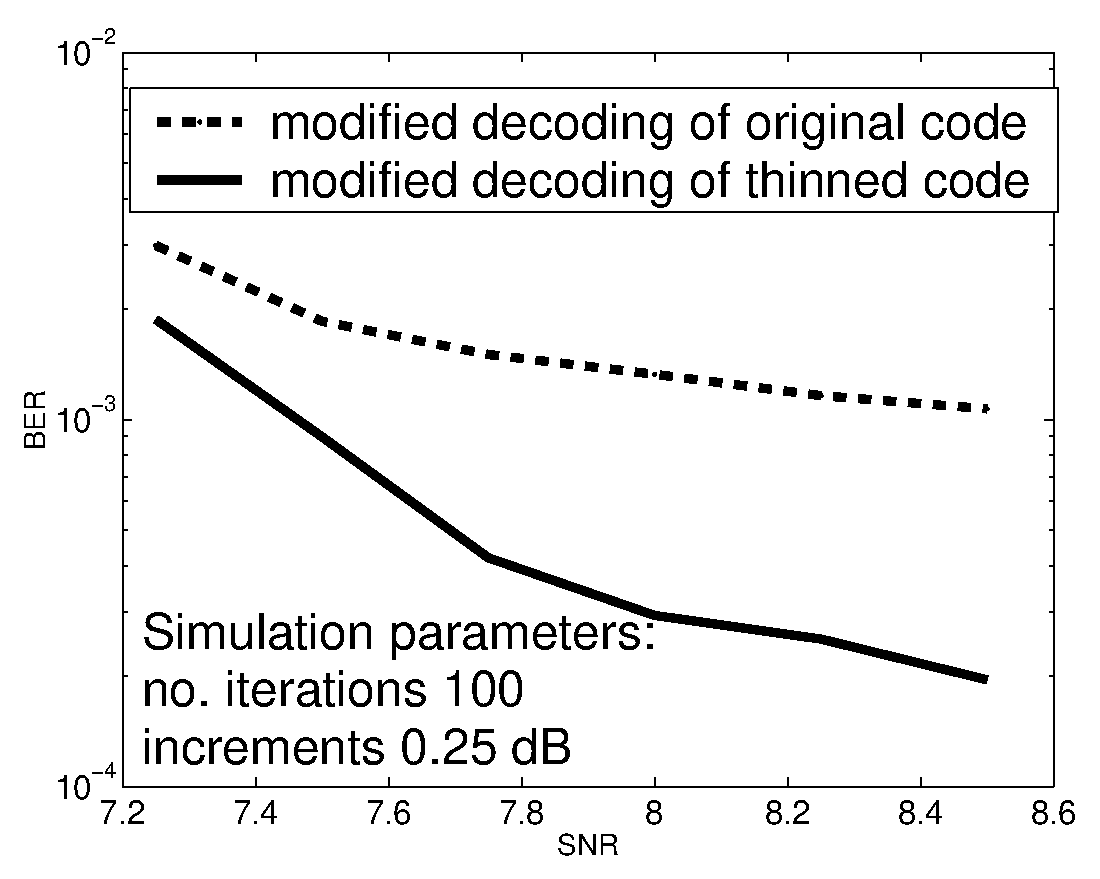
\includegraphics[width=2.5in,height=1.18in]{fig233b.eps}
\caption{Performance of LDPC (529,462) over AWGN with one
repetition} \vspace{-0.05in}
\end{figure}



\section{Concluding remarks}
We proposed a technique for modifying array-based LDPC codes when
varying sampling rate may cause repetition of symbols. Allowing a
small loss in rate, we systematically expurgate the code to get a
thinned code with significantly improved synchronization error
correction properties. We also gave a scheme for constructing
$t$-repetitions correcting families of sequences. Incorporating
multiple synchronization error correction capabilities in
array-based LDPC codes and other codes of interest is a topic for
future research.

% conference papers do not normally have an appendix

% use section* for acknowledgement
\vspace{-0.1in}
\section*{Acknowledgment}
% optional entry into table of contents (if used)
%\addcontentsline{toc}{section}{Acknowledgment}
The authors would like to thank Marvell Semiconductor Inc. and
U.C. MICRO program for supporting their research.



\begin{thebibliography}{17}

%\bibitem{Shannon1948}
%C. E. Shannon, ``A mathematical theory of communication,''
%\emph{Bell Syst.\ Tech.\ J.}, vol.\ 27, pt.~I, pp.~379--423, 1948;
%     pt.~II, pp.~623--656, 1948.
\bibitem{aji}
S. Aji and R. McEliece, ``The generalized distributive law",
\emph{IEEE Trans.  Inform. Theory} vol.\ 46(2), pp.~325--43, March
2000.
%\bibitem{tam}
%P. Bhagawat, M. Uppal and G. Choi, ``FPGA based implementation of
%decoder for array low-density parity check codes,''%In \emph{Proc. of
%\emph{ ICASSP}, 2005, pp.~29--32.%, Philadelphia, PA, USA.
%\bibitem{bours:94}
%P.A.H. Bours, ``Construction of fixed-length insertion/deletion
%correcting runlength-limited codes,'' \emph{IEEE Trans. Inf.
%Theory}, vol.\ 40(6), pp.~1841--1856, Nov. 1994.
\bibitem{cmnv:03}
G. Chen, M. Mitzenmacher, C. Ng and N. Varnica, ``Concatenated
codes for deletion channels,'' \emph{Int. Symp. Inform. Theory},
2003, p.~218.%, Yokohama, Japan.
\bibitem{dmackay:01}
M.C. Davey and D.J.C. MacKay, ``Reliable communication over
channels with insertions, deletions and substitutions,''
\emph{IEEE Trans. Inf. Theory}, vol.\ 47(2), pp.~687--98, Feb.
2001.
\bibitem{techArray:06} L. Dolecek and V. Anantharam, ``On array-based LDPC codes in channels
with varying sampling rate,'' available at
www.eecs.berkeley.edu/\~{}dolecek/papers
\bibitem{techRM:06} L. Dolecek and V. Anantharam, ``Using Reed-Muller codes in channels with synchronization and substitution errors,'' available at www.eecs.berkeley.edu/\~{}dolecek/papers
\bibitem{ibm:02} % linear time encoding    dsl app
E. Eleftheriou and S. \"{O}l\c{c}er, ``Low density parity check
codes for digital subscriber lines,'' \emph{Int. Conf. on Comm.},
2002, pp.~1752--57.
\bibitem{fan}
J. L. Fan, ``Array-codes as low-density parity-check codes,''
\emph{Second Int. Symp. on Turbo Codes and Related Topics}, 2000,
pp.~543--46.
%\bibitem{ferr:97}
%H.C. Ferreira, W.A. Clarke, A.S.J. Helberg, K.A.S. Abdel-Ghaffar and
%A.J. Han Vinck, ``Insertion/deletion correction with spectral
%nulls,'' \emph{IEEE Trans. Inf. Theory}, vol.\ 43(2), pp.~722--732,
%March 1997.
\bibitem{klove:95}
T. Kl{\o}ve, ``Codes correcting a single insertion/deletion of a
zero or a single peak-shift,'' \emph{IEEE Trans. Inf. Theory},
vol.\ 41(1), pp.~279--83, Jan. 1995.
\bibitem{kbek:04}
P. Kovintavewat, J. R. Barry, M. F. Erden and E. Kurtas,
``Per-survivor timing recovery for uncoded partial response
channels,''\emph{Int. Conf. on Comm.}, 2004, pp.~2715--19.%, Paris,
%France.
\bibitem{lev:66}
V. I. Levenshtein, ``Binary codes capable of correcting deletions,
insertions and reversals,'' \emph{Sov. Phys.-Dokl.}, vol.\ 10(8),
pp.~707--10, Feb. 1966.
\bibitem{liu:02}
J. Liu, H. Song and B.V.K.V. Kumar, ``Symbol timing recovery for
low-SNR partial response recording channels,'' \emph{Globecom}
2002, pp. 1129--36.%, San Francisco, CA, USA.
\bibitem{mittel:02}
T. Mittelholzer, ``Efficient encoding and minimum distance bounds
of Reed-Solomon-type array codes,'' \emph{Int. Symp. Inform.
Theory}, 2002, p. 282.%, Lausanne Switzerland.
\bibitem{mcla:02}
A. R. Nayak, J. Barry and S. W. McLaughlin, ``Joint timing
recovery and turbo equalization for coded partial response
channels,'' \emph{IEEE Trans. On Magnetics}, vol.\ 38(5),
pp.~2295--97, Sept. 2002.
\bibitem{sloane:00}
N.J.A. Sloane, ``On single deletion correcting codes,'' 2000.
Available at http://www.research.att.com/\~{ }njas/doc/dijen.pdf
\bibitem{kumar:04} %mr app
H. Song and B.V.K.V. Kumar, ``Low density parity check codes for
partial response channels,'' \emph{IEEE Signal Proc. Magazine},
vol.\ 21(1), pp.~56--66, Jan 2004.
\bibitem{vt:65}
R. R. Varshamov and G.M. Tenengolts, ``Codes which correct single
asymmetric errors,'' \emph{Avtomatika i Telemehkanika}, vol.\
26(2), pp.~288--92,1965.
\bibitem[17]{yanghell:03}
K. Yang and T. Helleseth, ``On the minimum distance of array codes
as LDPC codes," \emph{IEEE Trans. Inf. Theory}, vol.\ 49(12),
pp.~3268--71, Dec. 2003.
\end{thebibliography}

%%\documentclass[12pt]{article}
%\usepackage{amstext,amssymb}
%\usepackage{graphicx}
%\usepackage{times}
%\usepackage{psfig,latexsym}
%\usepackage{amstext,amssymb}
%\usepackage{amsmath}
%\begin{document}
%\newtheorem{theorem}{Theorem}
%\newtheorem{lemma}{Lemma}
%\newtheorem{corollary}{Corollary}
%\newtheorem{proposal}{Proposal}
\newcommand{\nchoosek}[2]{\left(\begin{array}{c}#1\\#2\end{array}\right)}
\chapter[Test Chapter]{Test Chapter}
Many communication systems use a substitution-error correcting
code to encode a binary input message $\mathbf{x}$ into a coded
sequence $\mathbf{c}$ = $C(\mathbf{x})$. The modulated version of
this sequence, corrupted by additive noise, arrives at the
receiver as a waveform $r(t)$,
\begin{equation}\label{eq:rt}
r(t)=\sum_{i} c_i h(t-iT) +n(t),
\end{equation}
where $c_i$ is the $i^{\text{th}}$ %$i^{\text{th}}$
bit of $\mathbf{c}$, $h(t)$ is the modulating pulse, and $n(t)$ is
the noise introduced in the channel.

Upon receiving $r(t)$, the receiver samples it at the times
$\left\{kT_s+\tau_k\right\} $. The samples are fed into the
decoder which produces the most likely input message. In
traditional correlation based receivers, for adequate noise
rejection, it is essential that the decoder be provided with
samples taken at approximately optimal time instances. As the
operating requirements under which timing recovery must be
performed become more stringent, such as lower signal to noise
ratio (SNR) and higher data rates, accurate synchronization
becomes critical for the full utilization of the available coding
gains. Several authors have proposed novel schemes which provide
ways of performing improved timing recovery \cite{liu:02},
\cite{kbek:04}.

When the adequate synchronization is missing, as a consequence of
the initial frequency error or of the accumulated phase error,
some symbol may be sampled more than once. Assuming that the exact
sampling instances are not known, a coded sequence $\mathbf{c}$
can give rise to a whole set of received sampled versions of
$r(t)$. When two distinct sequences $\mathbf{c_1}$ and
$\mathbf{c_2}$ result in the same sampled sequence, it is no
longer possible to uniquely determine the coded sequence or its
pre-image $\mathbf{x}$ from the received sequence, which can occur
even in the noise-free environment.

Codes that correct single insertion or a deletion of a bit were
investigated by Levenshtein in \cite{lev:66} and have been further
studied by Ferreira et al., \cite{ferr:97}, Levenshtein
\cite{lev:92}, Sloane \cite{sloane:00}, among others. Even though
these constructions assure that the code is immune to a deletion
or an insertion of a bit, they do not guarantee any other
desirable properties of standard substitution error correcting
codes, such as linearity and a good minimum Hamming distance.
Concatenated codes, with non negligible rate loss, that correct
synchronization errors have been proposed in \cite{cmnv:03} and
\cite{dmackay:01}.

We adopt a coding theoretic point of view in addressing inadequate
synchronization. We propose to focus on the encoding/decoding
components of the communication system and appropriately modify
these for better compensation of the inadequate synchronization.
The advantage of this approach lies in power and latency savings
over complex timing recovery schemes. The challenge lies in
appropriately modifying a code of interest without incurring
significant rate penalty for the benefit of improved
synchronization error correction capability. In our earlier work
\cite{isit06} we proposed a technique based on expurgation of
array-based LDPC codes which ensures immunity to single repetition
error.



In this paper we propose a general encoding method based on
extending an additive error correction code to include immunity to
multiple synchronization errors as follows. Suppose that $C$
denotes the additive error correction code used for transmission.
Let $\mathbf{c}$ denote a codeword in $C$, and let $n$ be the
codeword length. A binary string $\mathbf{p}$ of length $m$ is
prepended to the codeword $\mathbf{c}$ chosen for transmission,
and the resulting string $\mathbf{t}=[\mathbf{p}~ \mathbf{c}]$ is
sent over the channel. We assume that the channel is additive
white gaussian noise (AWGN). In addition, at most $s$ repetitions
are introduced as a consequence of imperfect timing recovery. As a
result, the receiver performs a decoding algorithm on a sequence
of length $n+m+s$, and its goal is to recover the original
sequence $\mathbf{c}$.

In Section \ref{construction} we present a construction of a
collection of strings immune to $s$ repetitions. Having
established several useful ancillary results in Section \ref{aux},
we then describe in Section \ref{enc} how to construct ``target''
string $\mathbf{t}$ used for transmission based on the codeword
$\mathbf{c}$ and the desired repetition-error correction
capability $s$. We show that, by judiciously applying the
construction in Section \ref{aux}, it is possible to achieve $m$
that is only $O(\log n)$. A decoding algorithm appropriate for
channels with $s$ repetitions and substitution errors based on
using LDPC codes is developed in Section \ref{dec}.



\section{Multiple Repetition Error Correcting
Code}\label{construction}

Let us first introduce a transformation in which we express the
number of runs of a string in terms of the weight of a string in
the transformed domain. For a string $\mathbf{c}$ of length $n$,
let the string $\tilde{\mathbf{c}}$ of length $n-1$ be defined as
$\mathbf{c}T_n$, where $T_n$ is a $n \times (n-1)$ matrix
satisfying\vspace{-0.0in}\begin{equation}\label{eq:t}T_{n}(i,j)=\left\{
\begin{array}{lll}
    1, & \text{if }i = j,j+1\\
    0, & \text{else.} \\
\end{array} \right. \end{equation}
If $\mathbf{c}$ has $r$ runs, then $\mathbf{\tilde{c}}$ has weight
$r-1$, and vice versa. Both $\mathbf{c}$ and its complement
$\mathbf{\overline{c}}$ result in the same $\mathbf{\tilde{c}}$.

 For
a prime number $P$, $P > m$, and an $s$-dimensional vector
$\underline{a}$ of residues mod $P$, let $S(\underline{a},m,P)$ be
the set of binary strings of length $m$ satisfying the following
set of congruency constraints:

\begin{equation}\label{eq1}\begin{array}{lll}S(\underline{a},m,P) = \{ & \mathbf{x}=(x_1, x_2, ... x_m) \in \{0,1\}^m
:\\ {} & \sum_{i=1}^{w(\mathbf{x})+1} f_ib_i \equiv a_1 \text{ mod } P,\\
{} & \sum_{i=1}^{w(\mathbf{x})+1} f_i^2b_i
\equiv a_2 \text{ mod } P,\\
{} & \hspace{0.5in}\vdots\\ {} & \sum_{i=1}^{w(\mathbf{x})+1}
f_i^sb_i \equiv a_s \text{ mod } P\},\end{array}\end{equation}

where $w(\mathbf{x})$ denotes the number of ones in $\mathbf{x}$,
$b_i$ is the number of zeros between the $i-1^{\text{st}}$ and
$i^{\text{th}}$ 1 in $\mathbf{x}$ (here $i=1$ run of zeros is
assumed to precede the leftmost 1 and $i=w(\mathbf{x})+1$ run of
zeros is assumed to follow the rightmost 1 in $\mathbf{x}$), $f_i$
is a ``weighting'' associated with $b_i$ such that each $f_i$
belongs to the residue set mod $P$ and $f_i \neq f_j$ for $i \neq
j$.


\begin{lemma}\textit{The set
$S(\underline{a},m,P)$ is s-insertions of zeros
correcting.}\end{lemma}

\textit{Proof}: Consider $\mathbf{x} \in$ $S(\underline{a},m,P)$.
After experiencing $s$ insertions of zeros, it becomes string
$\mathbf{x'}$. We now show that $\mathbf{x}$ is always uniquely
determined from $\mathbf{x'}$.


Let $i_1 \leq i_2 \leq ... \leq i_s$ be the (unknown) indices of
the bins of zeros that have experienced insertions. For each $j$,
$1\leq j \leq s$, compute $a_j'\equiv \sum_{i=1}^{w(\mathbf{x})+1}
f_i^jb_i' \text{ mod } P$, where $b_i'$ is the size of the
$i^{\text{th}}$ bin of zeros of $\mathbf{x'}$. Since we are
dealing with insertions of zeros, the weight of the string is
unchanged, $w(\mathbf{x'})$ = $w(\mathbf{x})$. Let
\begin{equation}\begin{array}{ll}
a_j'& \equiv \sum_{i=1}^{w+1} f_i^jb_i' \text{ mod } P\\
{}  & \equiv a_j + (f_{i_1}^j+f_{i_2}^j+...+f_{i_s}^j) \text{ mod
}P,
\end{array}
\end{equation}
where $a_j$ is the $j^{\text{th}}$ entry in the residue vector
$\underline{a}$.

By collecting the resulting expressions over all $j$, and setting
$R_j \equiv a_j'-a_j$ mod $P$, we arrive at
\begin{equation}
E_s=\left\{
\begin{array}{ll}
R_1 \equiv f_{i_1}+f_{i_2}+...+f_{i_s} \text{ mod }P\\
R_2 \equiv f_{i_1}^2+f_{i_2}^2+...+f_{i_s}^2 \text{ mod } P\\
\hspace{0.5in}\vdots\\
R_s \equiv f_{i_1}^s+f_{i_2}^s+...+f_{i_s}^s \text{ mod } P.\\
\end{array} \right.
\end{equation}
The terms on the right hand side of the congruency constraints are
known as power sums in $s$ variables. %Let $S_k$ denote the
%$k^{\text{th}}$ power sum mod $p_l$ of $\{i_1,i_2,...,i_t\}$,
%\begin{equation}
%S_k\equiv i_1^k+i_2^k+...+i_t^k \text{ mod }p_l,
%\end{equation}
%and
Let $\Lambda_k$ denote the $k^{\text{th}}$ elementary symmetric
function of  $\{f_{i_1},f_{i_2},...,f_{i_s}\}$ mod $P$,
\begin{equation}
\Lambda_k \equiv \sum_{v_1<v_2<...<v_k} f_{v_1}f_{v_2}\cdots
f_{v_k} \text{ mod } P.
\end{equation}
Using Newton's identities over $GF(P)$ which relate power sums to
symmetric functions of the same variable set, and are of the type
\begin{equation}\label{newton}
R_k-\Lambda_{1}R_{k-1}+\Lambda_{2}R_{k-2}-...+(-1)^{k-1}\Lambda_{k-1}R_{1}+(-1)^kk\Lambda_{k}
=0,
\end{equation}
for $k \leq s$, we can obtain an equivalent system of $s$
equations:
\begin{equation} \label{eq:dcoeff}
\widetilde{E}_s=\left\{
\begin{array}{ll}
d_1 \equiv \sum_{j=1}^s f_{i_j} \text{ mod }P\\
d_2 \equiv \sum_{j<k} f_{i_j} f_{i_k}\text{ mod }P\\
\hspace{0.5in}\vdots \\
d_s \equiv \prod_{j=1}^s f_{i_j} \text{ mod }P,
\end{array} \right.
\end{equation}
where each residue $d_k$ is computed recursively from
$\{d_1,...,d_{k-1}\}$ and $\{R_1,R_2,...,R_k\}$. This may be done
because, in each $k^{\text{th}}$ equation of the $s$ equations of
type (\ref{newton}) we use, the coefficient of $\Lambda_k$ is
nonzero.

Consider the expression:\vspace{-0.1in}
\begin{equation}\label{eq:p0} \prod_{j=1}^s(x-f_{i_j})\equiv 0 \text{ mod } P,
\end{equation}
and expand it into the form
\vspace{-0.1in}\begin{equation}\label{eq:p}
x^t+c_{t-1}x^{t-1}+...+c_1x+c_0 \equiv 0 \text{ mod } P.
\end{equation}
Since (\ref{eq:p0}) equals (\ref{eq:p}), by comparison with
(\ref{eq:dcoeff}) we see that $d_k \equiv (-1)^kc_{t-k} \text{ mod
} P$. We may then solve for the roots of (\ref{eq:p}) to get the
desired set of indices of weightings
$\{f_{i_1},f_{i_2},...,f_{i_s}\}$. Since different $f_{i_j}$'s
correspond to different bin indices, we may also recover the set
$\{{i_1},{i_2},...,{i_s}\}$, and from it the string $\mathbf{x}$
by deleting zeros from the bins of zeros indexed by the set
$\{{i_1},{i_2},...,{i_s}\}$. Hence $\mathbf{x}$ is always uniquely
recovered from $\mathbf{x'}$.$\hfill\blacksquare$

%
%As already mentioned, the weight of the transmitted string does not
%change during the transmission. Thus if one is interested in
%maximizing the size of the collection of strings capable of
%overcoming $s$ insertions of zeros using the above construction, one
%may partition the set $\{0,1\}^m$ by the weight. Then one can select
%the smallest prime $P_l$, $P_l>l$ in (\ref{eq1}) for each weight $l$
%(as opposed to a single $P$ for all weight groups).

Therefore, the pre-image of $S(\underline{a},n-1,P)$ under $T_n$
gives an $s$ repetitions correcting set.


\section{Auxiliary results}\label{aux}
We now prove some auxiliary results which will be used in the
following section on encoding.

\begin{lemma}\label{generates} For an integer $P$, each residue $r$ mod $P$ can be expressed as a
sum of a subset of elements of the set
$A_{z,P}=\{[z]_P,[2z]_P,[2^2z]_P,...,[2^{G}z]_P\}$ where
$G=\lfloor \log_2 P \rfloor $, $z$ is an arbitrary non zero
residue mod $P$ and the notation $[x]_P$ indicates the residue mod
$P$ congruent to $x$ .
\end{lemma}

\noindent \textit{Proof:} Observe that
$A_{1,P}=\{1,2,2^2,...,2^{G}\}$. We first show that each residue
$r$ mod $P$ can be expressed as a sum of a subset of elements of
the set $A_{1,P}$. Note that each residue $i$, $0 \leq i \leq
2^G-1$ (mod $P$) can be expressed as a sum of a subset, call it
$Q_i$, of the set $\{1,2,2^2,...,2^{G-1}\}$. Adding $2^G$ to the
sum of each $Q_i$, for $1 \leq i \leq 2^G-1$, generates the
residues $\{2^G, 2^G+1,...,P-1 \}\cup \{1,2,...2^G-1\}$. As a
result every residue mod $P$ can be expressed as a sum of a subset
of $A_{1,P}=\{1,2,2^2,...,2^{G}\}$.

Suppose there exists an element $r$ which cannot be expressed as a
sum of a subset of elements of $A_{z,P}$, for $z>1$, that is $r
\neq \sum_{i=0}^G \epsilon_i z 2^i \mod P$, for all choices of
$\{\epsilon_0,...,\epsilon_G\}$, $\epsilon_i \in \{0,1\}$. Then
the residue $r' = rz^{-1} \neq \sum_{i=0}^G \epsilon_i 2^i \mod
P$, for all choices of $\{\epsilon_0,...,\epsilon_G\}$,
$\epsilon_i \in \{0,1\}$, which contradicts the result from the
previous paragraph.\hfill$\blacksquare$

Suppose $P$ is a prime number such that $i|P-1$. Suppose the
equation $x^i\equiv a \mod P$ has a solution, $1 \leq a \leq P-1$.
Then the equation $x^i\equiv a \mod P$ has $i$ distinct solutions
\cite{apostol} and we may call them $x_1$ through $x_i$.
\begin{lemma}\label{sums}
The sum $\sum_{k=1}^i x_k^j \equiv 0 \mod P$ for $1 \leq j \leq
i-1$.
\end{lemma}
\noindent \textit{Proof:} Let us consider the equation $x^i \equiv
a \mod P$. Using Vieta's formulas over $GF(P)$ it follows that
$\Lambda_{j}=0$ for $0 \leq j \leq i-1$. Using Newton identities
over $GF(P)$ it then follows that
 $\sum_{k=1}^i x_k^j \equiv 0 \mod P$ for $1 \leq j \leq
i-1$.\hfill$\blacksquare$

For a prime number $P$ for which $i|P-1$, and $i<P-1$, let
$Q_i(P)$ be the set of distinct $i$th power residues mod $P$, let
$N_i(P)$ be the set of distinct $i$th power non residues mod $P$.
We also state the following convenient result.
\begin{lemma}\label{main}
Each $n \in N_i(P)$ can be expressed as a sum of two distinct
elements of $Q_i(P)$ in at least $P/(2k^2)-\sqrt{P}/2-3$ ways.
\end{lemma}
\noindent \textit{Proof:} The result follows from \cite{huavan:49}
which states that over $GF(P)$ the equation
\begin{equation}\label{hua} x^k+y^k=a
\end{equation} where $x,y,a \in GF(P)$ and nonzero and $0 < k <P-1 $
has at least $P-(k-1)^2\sqrt{P}-2(k-1)^2$ solutions. Noting that
$k$ distinct values of $x$ result in the same $x^k$, accounting
for the symmetry of $x$ and $y$, and omitting the case $x^k=y^k$
we obtain the lower bound on the number of solutions as
$P/(2k^2)-\sqrt{P}/2-3$. \hfill$\blacksquare$

Equations of the type in (\ref{hua}) were also studied by Weil
\cite{weil:49}.
\section{Encoding}\label{enc}

Let $s$ denote the target synchronization error correction
capability. The goal of this section it to provide an explicit
encoding scheme which based on the coded message $\mathbf{c}$
produces a fixed length prefix $\mathbf{p}$, where $\mathbf{p}$ is
a function of $\mathbf{c}$, such that the string $\mathbf{t}=[
\mathbf{p} ~ \mathbf{c} ]$ satisfies first $s$ congruency
constraints previously described (used for the recovery from
synchronization errors) in section~\ref{construction}. Using
judiciously chosen prefix, we will show that this will be possible
for $m=|\mathbf{p}|=O(\log n)$. As a result the transmitted string
will have asymptotically negligible rate loss compared to the
starting code $C$ while providing improved immunity to
synchronization errors.

 Let $w$ be
the design parameter, $w \in \mathbb{N}$, which determines the
sizes of the bins in the the substring $\mathbf{p}$ of
$\mathbf{t}$ under $T_{m+n}$ transformation. This parameter will
be exploited in the decoding of the $\mathbf{p}$ string, as
explained in Section~\ref{dec}.

 Let $P$ be a prime number chosen such that $P$ is
$c_1n < P< c_2n$, for appropriately chosen constants $c_1$ and
$c_2$.  We choose $c_1$ such that $c_1n>n+s(s+1)(\lfloor\log
P\rfloor+1)$ and $c_2$ sufficiently large such that
$lcm(2,3,\dots,s)|P-1$.


 We
construct $\mathbf{p}$ of length $m$ such that in
$\mathbf{\tilde{t}}=[\mathbf{p}~ \mathbf{c}]T_{m+n}$ the leftmost
substring $\mathbf{\tilde{t}}(1,m)$ (here and in the remainder
$\mathbf{x}(p,q)$) denotes a substring of $\mathbf{x}$ spanning
positions $p$ and $q$) has weight \begin{equation}\label{sum1}
1+\sum_{i=1}^s i\left[ 2(G+1)-\lceil(G+1)/i \rceil
\right]\end{equation} and ends in `1'. Since the pre-image under
$T_m$ contains two strings (which are complements of each other)
we let $\mathbf{p}$ be the one for which
$\mathbf{p}(n)=\overline{\mathbf{c}(1)}$ (here and in the
remainder $\mathbf{x}(q)$ denotes the bit in the $q^{\text{th}}$
position in $\mathbf{x}$, and $\overline{\mathbf{x}(q)}$ denotes
the complement of the bit $\mathbf{x}(q)$). %As a result the
%$(G+2)^{\text{st}}$ bin in $\mathbf{t}$ is fully contained in the
%substring $\mathbf{p}$, and the $(G+3)^{\text{nd}}$ run in
%$\mathbf{t}$ is fully contained in the substring $\mathbf{c}$.
Let $b_i$ is the number of zeros between the $(i-1)^{\text{st}}$
and $i^{\text{th}}$ 1 in $\mathbf{\tilde{t}}$. This run of zeros
will be referred to as the $i^{\text{th}}$ bin. Let $M$ be the
total number of bins in $\mathbf{\tilde{t}}$.


%Since $\mathbf{p}(n)=\overline{\mathbf{c}(1)}$, the
%${G+2}^{\text{nd}}$ bin is fully contained in the
%$\mathbf{\tilde{p}}$ portion of $\mathbf{\tilde{t}}$, and likewise
%the ${G+3}^{\text{nd}}$ bin is fully contained in the
%$\mathbf{\tilde{c}}$ portion of $\mathbf{\tilde{t}}$.





Let $R(P)$ denote the reduced set of residues mod $P$. For each
$i, 1 \leq i \leq s$, since $i | P-1$ by construction, $Q_i(P)$ is
of size $(p-1)/i$ \cite{apostol}. Consider the set
$A_{z_i,P}=\{[z_i]_P,[2z_i]_P,[2^2z_i]_P,...,[2^{G}z_i]_P\}$ where
$G=\lfloor \log_2 P \rfloor $ and $z_i \in Q_i(P)$. By Lemma
\ref{generates} each residue in $R(P)$ can be written as a linear
combination of some elements in $A_{z_i,P}$.

Moreover, each element in $A_{z_i,P}$ either belongs to $Q_i(P)$
or, if not, can be expressed as a sum of two distinct elements of
$Q_i(P)$ in at least $P/(2i^2)-\sqrt{P}/2-3$ ways by Lemma
\ref{main}. Replace each $i$th power non residue $x$ in
$A_{z_i,P}$ by two $i$th power residues, the sum of which is $x$,
and such that no  $i$th power residue participates in the sum of
more than  one such element, and such that itself is not an
original element of $A_{z_i,P}$. Let $Y_i(z_i)$ be the resulting
set. It is of size $2(G+1)-\lceil (G+1)/i \rceil$. We have thus
obtained the set $Y_i(z_i)$ of size $O(\log P)$ and such that all
elements in $R(P)$ can be expressed as a linear combination of
elements of $Y_i(z_i)$, by Lemma \ref{generates}.

Let $V_i(z_i)$ for $1 \leq i \leq s$ be such that each $V_i(z_i)$
is of size $i \times Y_i(z_i)$ and contains all $ith$ roots of
elements of $Y_i(z_i)$. Select $z_1$ through $z_s$ such that
$V_i(z_i) \cap V_j(z_j) = \emptyset$ for $i \neq j, 1 \leq i,j
\leq s $, which is possible for $P$ large enough. Along with the
zero weighting, the elements of $V_i(z_i)$ for $1 \leq i \leq s$
are reserved to be weightings of the first
$|V_1(z_1)|+\dots+|V_s(z_s)|+1$ bins in $\mathbf{t}$ which are
made to entirely and only arise from runs in $\mathbf{p}$. Note
that for $\mathbf{\tilde{p}}$ the number of bins equals the
weight, which is (\ref{sum1}), as required. For notational
simplicity let $L=|V_1(z_1)|+\dots+|V_s(z_s)|+2$.



 Let
\begin{eqnarray}\label{code1} {a'}_1 &\equiv& \sum_{i=L}^M b_i f_i
\text{ mod } P, \\ {a'}_2 &\equiv& \sum_{i=L}^M b_i f_i^2 \text{
mod } P\\ &\vdots& \\
\label{codes}{a'}_s &\equiv& \sum_{i=L}^M b_i f_i^s \text{ mod }
P\end{eqnarray}

where $f_i$ in (\ref{code1}) through (\ref{codes}) are chosen in
the increasing order from the set $R(P)\setminus \{V_1(z_1) \cup
\dots \cup V_s(z_s) \}$, which is possible by the lower bound on
$P$. Note that $M-L+1 \leq n $. We may think of ${a'}_1$ through
${a'}_s$ as the contribution of the codeword to the overall
congruency value. We now show that it is always possible to
achieve
\begin{eqnarray}\label{s1} a_1 &\equiv& \sum_{i=1}^M b_i f_i
\text{ mod } P, \\ a_2 &\equiv& \sum_{i=1}^M b_i f_i^2 \text{
mod } P\\ &\vdots& \\
a_s &\equiv& \sum_{i=1}^M b_i f_i^s \text{ mod }
P\label{s2}\end{eqnarray}

for arbitrary but fixed values $a_1$ through $a_s$ irrespective of
the values ${a'}_1$ through ${a'}_s$, where $b_i$ is either $0$ or
$w$ for $1 \leq i \leq L-1$, and where $f_L=0$.

The encoding is recursive and proceeds as follows.

Let $l$ be the $l$th level of recursion for $l=1$ to $l=s$. The
$l$th level ensures that the $l$th congruency constraint is
satisfied without altering previous $l-1$ levels.
 At each level $l$, starting with $l=1$ and while $l \leq s$:
\begin{enumerate}
 \item Select a subset $F_{l}$ of $V_l(z_l)$ such that $\sum_{k \in F_l} k^lw \equiv a_l - {a'}_l -
\sum_{i=1}^{l-1} d_{i,l} \mod P$. (For $l=1$, $\sum_{k \in F_1} kw
\equiv a_1 - {a'}_1 \mod P$.)\item Let $d_{l,j} \equiv \sum_{k \in
F_l} k^jw \mod P$ for $l+1 \leq j\leq s$. \item For each $i$, $1
\leq i \leq |V_l(z_l)|$, for which $f_i \in F_l$ we set $b_i=w$,
and for each $i$, $1 \leq i \leq |V_l(z_l)|$, for which $f_i
\notin F_l$ we set $b_i=0$, where $w$ is a fixed integer $w \geq
1$. \item Proceed to level $l+1$.
\end{enumerate}

After the level $s$ is completed, let $b_L=w(\sum_{i=1}^s
|V_i(z_i)|- |F_{i}|)$. The purpose of this bin with weighting zero
is to ensure that the overall string $\mathbf{t}$ has the same
length irrespective of the structure of the starting codeword
$\mathbf{c}$.

The existence of $F_l, F_l \subseteq V_l(z_l)$ in Step 1) follows
from Lemma~\ref{generates} and Lemma~\ref{main}. Observe that by
Lemma~\ref{sums} the contribution to each congruency sum for
levels $1$ through $l-1$ of the elements of $F_l$ is zero. Hence,
once the target congruency value is reached for a particular
level, it will not be altered by establishing congruencies at
subsequent levels.
\section{Decoding}\label{dec}

Assume that based on a codeword $\mathbf{c}$ a string
$\mathbf{t}=[\mathbf{p} ~ \mathbf{c}]$ is constructed using the
encoding procedure outlined above, such that $\mathbf{t}$
satisfies (\ref{s1}) through (\ref{s2}). Assume that $\mathbf{t}$
is transmitted over an AWGN channel, which in addition introduces
$s$ repetitions. The received sequence $\mathbf{r}$ is of length
$|\mathbf{t}|+s$ bits.

The decoding consists of the following steps:
\begin{enumerate}
\item Decode $\mathbf{p}$ portion of $\mathbf{r}$. \item Determine
the contribution of  $\mathbf{p}$ to (\ref{s1}) through
(\ref{s2}). \item Decode $\mathbf{c}$ portion of $\mathbf{r}$.
\item Determine the contribution of  $\mathbf{c}$ to (\ref{s1})
through (\ref{s2}) and if consistent with the target values $a_1$
through $a_s$, declare successful decoding.
\end{enumerate}

In particular:

Step (1). By construction, all but one run in $\mathbf{p}$ is
either of length $1$ or $w+1$. Upon receiving corrupted version of
$\mathbf{p}$ we may perform brute force search to find the most
likely $\mathbf{\hat{p}}$ since its length is only logarithmic in
the codeword length by construction.

Step (2). Compute $\hat{a}^{''}_k \equiv \sum_{i=1}^{L-1}
\hat{b}_i \hat{f}_i^k \mod P$ for $1\leq k \leq s$, where
$\hat{b}_i$ and $\hat{f}_i$ are obtained from $\mathbf{\hat{p}}$.

Step (3). We introduce auxiliary variables $G$, an $s$-dimensional
vector $(g_1,\dots,g_s)$ which takes values $\in \{1,...,n\}^s$,
and $L_i$, for $\forall$ $i \in [1,n]$, such that $L_i \in
\{-s,-s+1,...,-1,0,1,...,s-1,s\}$. The variable $G$ denotes the
positions of the repetitions, and $L_i$ denotes the relative
location of the $i^{\text{th}}$ bit with respect to the
repetitions. Let $\mathbf{y}_1^{n+s}=\mathbf{r}_{m+1}^{m+n+s}$.

Write \begin{equation}\label{marg}P(x_i| \mathbf{y}_1^{n+s}) =\\
\sum_G \sum_{L_1^n} \sum_{x_1^n \backslash x_i} P(x_1^n,L_1^n,G
|\mathbf{y}_1^{n+s}).\end{equation}

Group the variables as shown in Fig. 1., for $1 \leq i \leq n$ and
$1 \leq k \leq M_c$, where $M_c$ is the total number of checks.
Note that $\mathbf{y}_1^{n+s}$ is viewed as evidence.
\begin{figure}\label{ta1}
\hspace{-0.0in}\small\begin{tabular}{|c|c|}
  \hline
  % after \\: \hline or \cline{col1-col2} \cline{col3-col4} ...
   \text{local domain} & \text{local function} $\varphi(\cdot)$\\
  \hline
   $\{G\}$ & 1 \\\hline
   $\{G,L_i\}$ & $1\left[L_i=s\cdot 1(g_1<...<g_s\leq i-1)+\right.$\\
   {} & $\left. +\dots +L_i=-s\cdot 1(g_s>...>g_1\geq i+1)\right]$\\
   \hline
   $\{L_i,x_i\}$ &
   $P(y_i|x_i)1(L_i=-s)$+\\{} & $P(y_i|x_i)P(y_{i+1}|x_i)1(L_i=-s+1)+...+$\\
   {} & $P(y_{i+s-1}|x_i)P(y_{i+s}|x_i)1(L_i=s-1)$\\{}&+$P(y_{i+s}|x_i)1(L_i=s)$\\\hline
   $\{x_i\}$ & 1\\\hline
   $\{c_k,(x_j,j \in \mathcal{N}_k)\}$ & $1(c_k =\oplus_{j \in
   \mathcal{N}_k} x_j)$\\
  \hline
\end{tabular}\caption{Local domains and functions for Step 3.}
\end{figure}

The junction graph corresponding to these local domains is shown
in Fig. 2, and has the bidirectional edges between:\begin{itemize}
\item $\{G \}$ and $\{G, L_i\}$ for each $1 \le i \le n$, \item
$\{G, L_i\}$ and $\{ L_i, x_i\}$ for each $1 \le i \le n$,  \item
$\{ L_i, x_i\}$ and $\{c_k, (x_i, i \in {N}_k )\}$, for each pair
$(i,k)$ such that $i \in {N}_k$, and \item $\{x_i\}$ and
$\{L_i,x_i\}$ for each $1 \le i \le
n$.\end{itemize} %Then,

%\begin{equation}\hspace{0.4in}\label{joint}\begin{array}{ll}
%\sum_G \sum_{L_1^n} \sum_{x_1^n \backslash x_i}
%P(x_1^n,L_1^n,G,y_1^{n+1}) \approx
%\\\hspace{-0.4in} \sum_{L_i} \varphi(L_i,x_i)\sum_G\varphi(G,L_i)\prod_{j=1,j
%\neq i}^n  \sum_{L_j} \varphi (G,L_j) \\ \times \sum_{x_j}
%\varphi(L_j,x_j) \prod_{k \in \mathcal{N}_i} 1(c_k =\oplus_{j \in
%   \mathcal{N}_k} x_j)\vspace{-0.1in}\end{array}\end{equation}
%where $\varphi(\cdot)$ denotes the local function of the appropriate
%variables listed in Fig.1 and the approximation comes from ignoring
%the cycles in the graph.

\begin{figure}
%\vspace{0.0in}\hspace{0.0in}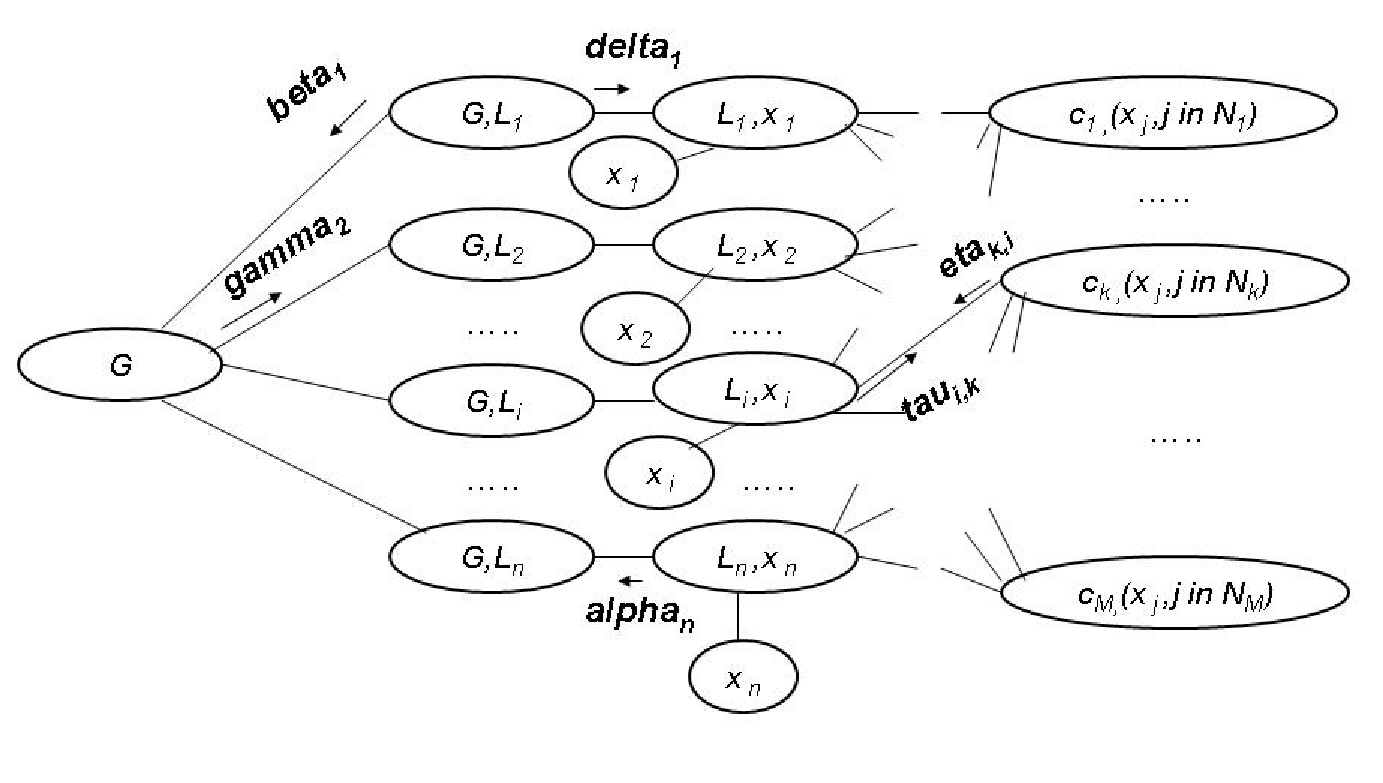
\includegraphics[width=3.0in,height=1.9in]{fig7.eps}
\caption{Junction graph for Step 3.}
\end{figure}

Observe that
\begin{equation}\begin{array}{lll}
P(x_1^n,L_1^n,G|\mathbf{y}_1^{n+s}) \propto \\\varphi(G) \prod_{i}
\varphi(G,L_i) \prod_{i} \varphi(L_i,x_i) \prod_i\varphi(x_i)
\prod_k \varphi(c_k,(x_j, j \in \mathcal{N}_k)).\end{array}
\end{equation}

We may use a message passing algorithm as in \cite{aji} to try to
evaluate  $P(x_i|\mathbf{y}_1^{n+s})$.

Let all messages be initialized to 1, and let $\alpha_j(L_j)$ be
the message sent from $\{L_j,x_j\}$ to $\{G,L_j\}$ at some stage.

The message $\beta_j(G)$ from $\{G,L_j\}$ to $\{G\}$ is then
$\beta_j(G)=\sum_{L_j}\varphi (G,L_j)\alpha_j(L_j)$, and the
message $\gamma_i(G)$ sent from $\{G\}$ to $\{G,L_i\}$ is
$\prod_{j \in \{1,n\}\backslash i} \beta_j(G)$. Finally, the
message from $\{G,L_i\}$ to $\{L_i,x_i\}$ is
$\delta_i(L_i)=\sum_G\varphi(G,L_i)\gamma_i(G)$.

The message $\tau_{j,k}(x_j)$ sent from $\{L_j,x_j\}$ to $\{c_k
(x_j, j \in \mathcal{N}_k)\}$ is $\sum_{L_j}\varphi(L_j,x_j)
\delta_j(L_j)\prod_{l \in \mathcal{N}_j \backslash k}
\eta_{l,j}(x_j)$, where $\eta_{l,j}(x_j)$ is the message from
$\{c_l,(x_j, j\in \mathcal{N}_l)\}$ to $\{L_j,x_j\}$ and is
$\sum_{x_i,i\in \mathcal{N}_l\backslash j}\varphi(c_l, (x_i, i \in
\mathcal{N}_l)) \prod \tau_{i,l}(x_i).$

The message $\alpha_j(L_j)$ is updated to $\sum_{x_j}
\varphi(L_j,x_j) \prod_{k \in \mathcal{N}_j}\eta_{k,j}(x_j)$, and
message exchange continues as above.

As a result, from (\ref{marg}) one gets \begin{equation}P(x_i|
\mathbf{y}_1^{n+s}) \approx
\sum_{L_i}\varphi(L_i,x_i)\delta_i(L_i)\prod_{k \in \mathcal{N}_i}
\eta_k (x_i),\end{equation} and we also have
\begin{equation}
P(G=\underline{g}|\mathbf{y}_1^{n+s}) \approx \prod_{i=1}^n
\beta_i(\underline{g}).
\end{equation}
Even though there are $O(n)$ computations each involving $O(n)$
variables per global iteration step, computational complexity can
be reduced from $O(n^2)$ to $O(n)$ with appropriate organization
of calculations. In particular, $\delta$'s can be computed
directly from $\alpha$'s. For details please see \cite{tech:07}.


The messages $\tau_{j,k}$ and $\eta_{k,j}$ are analogous to
messages computed in a traditional message passing algorithm on a
bipartite graph, so their complexity is also $O(n)$.

Step (4). Compute $\hat{a}'_k \equiv \sum_{i=L}^{M} \hat{b}_i
\hat{f}_i^k \mod P$ for $1\leq k \leq s$, where $\hat{b}_i$ and
$\hat{f}_i$ are obtained from $\mathbf{\hat{c}}$. If
$\hat{a}'_k+\hat{a}^{''}_k \equiv a_k \mod P$ for $1\leq k \leq s$
declare successful decoding.
\subsection{Simulation results}
To be filled in-in progress.\vspace{0in}
\section{Concluding remarks}
We proposed a technique for modifying additive error correction
codes when varying sampling rate causes repetition of symbols. We
presented an encoding scheme which relies on introducing a
carefully chosen prefix such that the overall string (consisting
od the prefix and the codeword) is immune to repetition errors.
The prefix length is only logarithmic in the codeword length. We
also gave a companion message passing algorithm suitable for
decoding of LDPC codes under multiple repetitions and with such a
prefix.

\section*{Acknowledgment}
% optional entry into table of contents (if used)
%\addcontentsline{toc}{section}{Acknowledgment}
The authors would like to thank Marvell Semiconductor Inc. and
U.C. MICRO program for supporting their research.

\begin{thebibliography}{10}
\bibitem{aji}
S. Aji and R. McEliece, ``The generalized distributive law",
\emph{IEEE Trans.  Inform. Theory} vol.\ 46(2), pp.~325--43, March
2000.
\bibitem{apostol} T. M. Apostol, ``\emph{Introduction to Analytic Number
Theory}'', Springer-Verlag, NY, 1976.
\bibitem{cmnv:03}
G. Chen, M. Mitzenmacher, C. Ng and N. Varnica,``Concatenated
codes for deletion channels,'' In \emph{Proc. of the IEEE
International Symposium on Information Theory} 2003, Yokohama,
Japan, p.~218.
\bibitem{dmackay:01}
M.C. Davey and D.J.C. MacKay, ``Reliable communication over
channels with insertions, deletions and substitutions,''
\emph{IEEE Trans. on Information Theory} vol.\ 47(2), pp.~687-698,
Feb. 2001.
\bibitem{isit06} L. Dolecek and V. Anantharam, ''A synchonization
technique for array-based LDPC codes'', \emph{Int. Symp. on
Information Theory}, Seattle, WA, 2006.
\bibitem{tech:07} L. Dolecek and V. Anantharam, ``On reliable communication over channels
with varying sampling rate,'' available at
www.eecs.berkeley.edu/\~{}dolecek/papers
\bibitem{ferr:97}
H.C. Ferreira, W.A. Clarke, A.S.J. Helberg, K.A.S. Abdel-Ghaffar
and A.J. Han Vinck, ``Insertion/deletion correction with spectral
nulls,'' \emph{IEEE Trans. on Information Theory} vol.\ 43(2),
pp.~722--732, March 1997.
\bibitem{huavan:49}
L. K. Hua and H. S. Vandiver, ``Characters over certain types of
rings with applications to the theory of equations in a finite
field'', \emph{Proc. Nat. Acad. Sci. USA}, vol. 35, pp.~481-487,
1949.
\bibitem{lev:66}
V. I. Levenshtein,``Binary codes capable of correcting deletions,
insertions and reversals,'' \emph{Sov. Phys.-Dokl.}, vol.\ 10(8),
pp.~707--710, Feb. 1966.
\bibitem{lev:92}
V. I. Levenshtein, ``On perfect codes in deletion and insertion
metric,'' \emph{Discrete Math. Appl.}, vol.\ 2(3), pp.~241--258,
1992.
\bibitem{liu:02}
J. Liu, H. Song and B.V.K.V. Kumar, ``Symbol timing recovery for
low-SNR partial response recording channels," In \emph{Proc.
GLOBECOM 2003}, Nov. 2002, pp. 1141 -- 1145, San Francisco, CA,
USA.
\bibitem{kbek:04}
P. Kovintavewat, J. R. Barry, M. F. Erden and E. Kurtas,
``Per-survivor timing recovery for uncoded partial response
channels,''\emph{Proceedings of the IEEE International Conference
on Communications} 2004, Paris, France.
\bibitem{sloane:00}
N.J.A. Sloane, ``On single deletion correcting codes,'' 2000.
Available at http://www.research.att.com/\~{ }njas/doc/dijen.pdf
\bibitem{weil:49}
A. Weil, ''Numbers of solutions of equations in finite fields", in
\emph{Bull. Amer. Math. Soc}, vol. 50, pp.~497--508, 1949.
\end{thebibliography}
%\end{document}

\part[Iterative Decoding of LDPC Codes]{Iterative Decoding of LDPC
Codes}
\chapter[Introduction]{Introduction}\label{introb}

In this part of the thesis we are concerned with the analytic
understanding of the LPDC code performance under iterative decoding,
with the particular focus on the performance of finite-length LDPC
codes in the low BER region.

Low density parity check (LDPC) codes are a class of error control
codes defined on sparse graphs \cite{gallager}. Their graphical
representation makes them particularly amenable for low-complexity
iterative decoding algorithms. LDPC codes were invented by Gallager
\cite{gallager} in the 1960's, but then were largely forgotten until
early 1990's. Their rediscovery \cite{mackay96}, \cite{foss01}
ignited intensive research in LDPC codes, as well as their wide
consideration for many modern applications.

While vast empirical evidence points to the successful use of LDPC
codes, most of the known theoretical results regarding the
performance of LDPC codes are asymptotic in nature. A theoretical
tool known as density evolution \cite{richurbanke} operates on an
infinitely long LDPC code ensemble and it demonstrates an
exponential concentration of the messages exchanged in the decoding
process around their mean. The underlying assumption in density
evolution is that a large enough neighborhood of each node is
locally tree-like, which can be assumed as the block length tends to
infinity. However, for finite-length LDPC codes (with block lengths
on the order of hundreds or thousands) such assumption no longer
holds, and in fact for structured finite-length LDPC codes there
inevitably exist numerous relatively short cycles in the associated
Tanner graph. Furthermore, in this finite blocklength regime, many
LDPC codes exhibit a so-called ``error floor", corresponding to a
significant flattening in the curve that relates signal to noise
ratio (SNR) to the bit error rate (BER) level, typically occurring
in the low BER region. Since moderate blocklengths and low BER's are
of primary interest in many communications and data storage
applications, prior lack of understanding of the LDPC code
performance has significantly hindered the wide-scale deployment of
these very promising codes.

In this dissertation we aim to address this issue through the
introduction and the subsequent study of a convenient combinatorial
object, which we have termed an absorbing set.

 \comment{While vast empirical evidence points to the
successful use of LDPC codes, most of the known theoretical results
regarding the performance of LDPC codes are asymptotic in nature. A
theoretical tool known as density evolution \cite{richurbanke}
demonstrates an exponential concentration of the messages exchanged
in the decoding process around their mean for an LDPC code ensemble.
The underlying assumption in the density evolution is that a large
enough neighborhood of each node is locally tree-like, which implies
that the message passing algorithms, known to be equivalent to the
maximum likelihood decoding on graphs that are trees, can be
successfully applied. This theory however cannot be directly applied
to specific medium sized LDPC codes that intrinsically have
structure and thus many relatively short cycles since the structure
itself  is typically a key feature for an efficient, high-throughput
implementation of an LDPC decoder~\cite{zhang06}. Since these
finite- length, structured LDPC codes are of primary interest in
most modern applications, the lack of theoretical tools needed to
understand the LDPC code performance for finite block lengths has
also meant that the wide spread deployment of these code has not yet
quite met the original promise, despite the unprecedented coding
gains associated with certain LDPC codes \cite{chung}.}

\comment{In addition to the lack of adequate theory to explain the
performance of finite length LDPC codes for the low frame error
rates (FER), the inability to simulate these codes in a reasonable
time frame in the low FER regimes, has also limited our
understanding of the LDPC code performance. As a concrete example,
months of simulation time would be required to estimate the
performance at FER of $10^{-10}$, which is itself the region in
which modern storage and wireline communications systems aim to
operate.

Thus, an important open problem in modern coding theory is that of
understanding the performance of finite-length low density parity
check (LDPC) codes, particularly in the low BER region.}

The following chapter provides the background on the low BER
performance of LDPC codes, where we discus the error floor,
introduce the notion of an absorbing set and summarize some related
work. Later, we will provide an in-depth study of absorbing sets for
an important family of high-performance finite-length LDPC codes.

\chapter[Background on Iterative Decoding]{Background on Iterative
Decoding}\label{iterativeBG}

In this chapter we focus on the LDPC code performance in the low BER
region, and discuss the so-called ``error-floor" phenomenon. We
introduce the combinatorial object termed absorbing set, and relate
it to some existing concepts form the literature. Having defined an
absorbing set, in the next chapter we focus on the detailed
theoretical analysis of absorbing sets for a family of high-rate
array-based LDPC codes.

\section{LDPC Codes, Message Passing Algorithms and Error Floors}

 Empirically,
LDPC codes perform very well when decoded iteratively using
message passing algorithms, despite the fact that such decoding
algorithms are suboptimal on graphs with cycles (and graphs
defining LDPC codes inevitably contain cycles). An added
attractive feature of message passing algorithms is their low
complexity.

However, it is also known \cite{mackay}, \cite{richardson}, that
LDPC codes often exhibit an error floor phenomenon, whereby the bit
error rate (BER) vs. signal to noise ratio (SNR) curve shows a
significant decrease in the slope in the very low BER region. An
example of the error-floor behavior is shown in
Figure~\ref{errorfig} (reproduced from \cite{zhang06}) for the
Reed-Solomon based LDPC code, where different error curves
correspond to specified number of iterations. The error floor
implies that a significant increase in the signal power is needed
for only a marginal improvement in the bit error rate. It is
attributed to the suboptimal nature of the message passing
algorithms on graphs with cycles.

For many applications, including data storage, gigabit ethernet, and
satellite communications, it is imperative to reach this low BER
region without requiring a major increase in SNR. This region,
however, is out of the reach of pure software simulations, and
consequently the limitations of a given LDPC code under
message-passing decoding in the very low BER region are largely
unknown.

In order to explain and analyze the dominant causes of decoding
failures we introduce the notion of an absorbing set in the next
section. The absorbing sets are related to (but not entirely
equivalent to) previously introduced structures, including stopping
sets \cite{di_stop}, trapping sets \cite{richardson}, near codewords
\cite{mackay} and pseudo-codewords \cite{wainwrig}. Fully absorbing
sets are viewed as fixed points of a bit-flipping algorithm (which
itself is a simplest form of message passing and can be viewed as a
1-bit approximation to the finite-precision message passing decoding
algorithms that are used in practice). Our claim is that if there
are fully absorbing sets smaller that the minimum distance of the
code, the decoder is likely to converge to these objects. As a
result, under iterative decoding, the low BER performance will be
dominated by the number and the size of dominant fully absorbing
sets. This is in contrast to the conventional point of view which
considers the number of minimum distance codewords and the minimum
distance itself to be the key performance metric of a code.


\begin{figure}
\center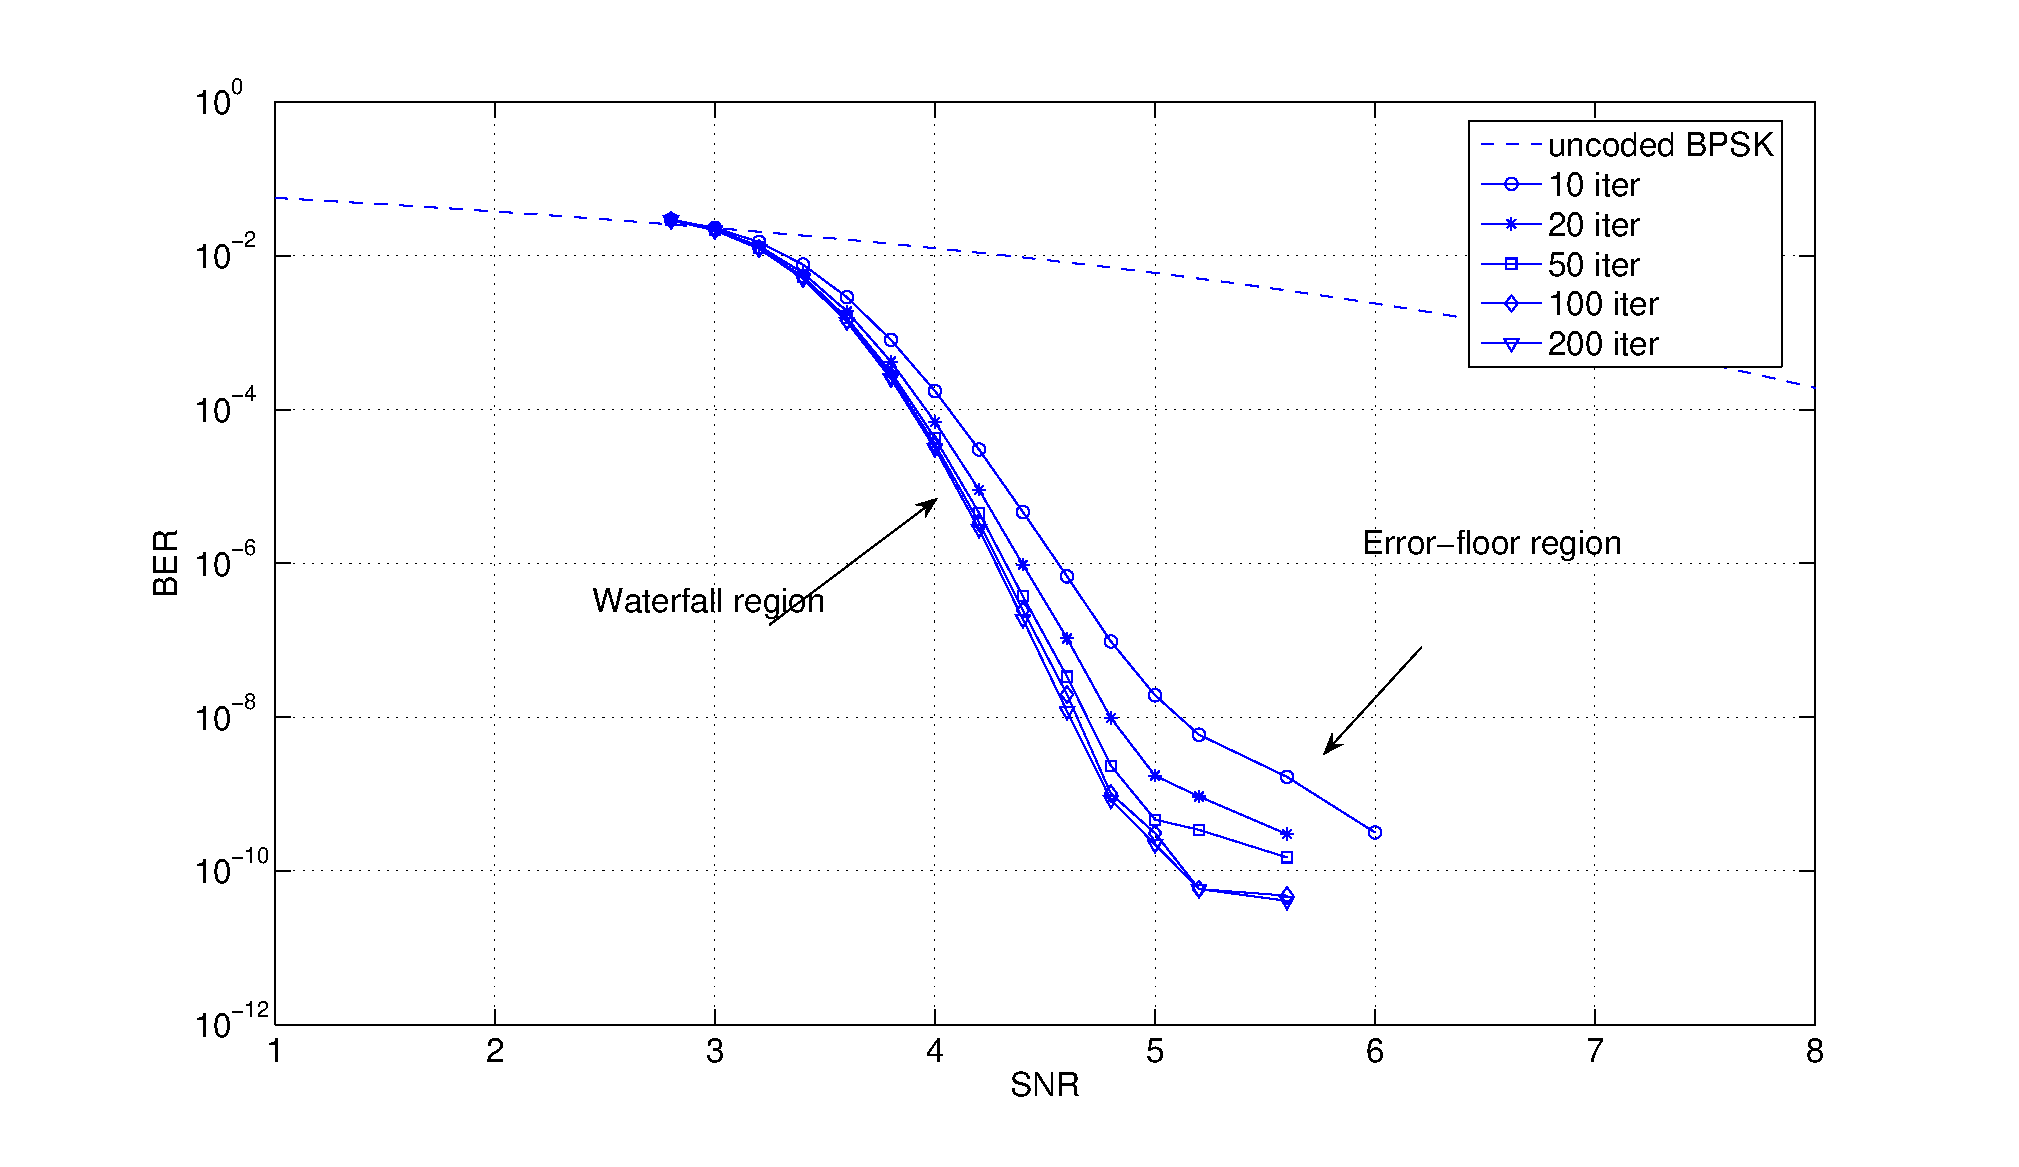
\includegraphics[width=4.75in,keepaspectratio]{iter_globecom3.ps}
\caption{An example of error floor.} \label{errorfig}
\end{figure}


\section{Absorbing sets of LDPC codes}


Several LDPC codes, while having excellent performance for
moderate bit error rate (BER) levels of $10^{-6}$ and above, have
been demonstrated using hardware based emulation \cite{zhang06}
and software clusters \cite{cluster} to suffer from the so-called
``error floor'', see Figure \ref{errorfig}.

This error-floor behavior can be attributed to the suboptimal
nature of the message passing
 algorithms traditionally used in decoding of LDPC codes. Experimental results in
 the low FER region obtained using a hardware emulator
 \cite{zhang06} revealed  that certain structures consisting of short cycles
 organized in particularly detrimental configurations in the Tanner
 graph associated with the parity check matrix of an LDPC code
 cause the decoder to fail by converging to a non-codeword state.


These combinatorial objects that describe the convergence to the
non-codeword state  are called \textit{absorbing sets}. For many
LDPC codes, designed to have sufficiently large minimum distance,
the associated Tanner graphs contain absorbing sets which have
strictly fewer bits than the weight of codewords at the minimum
distance. As a result, the performance of the decoding algorithm
in the low FER region is predominantly dictated by the number and
the structure of minimal absorbing sets, rather than the number of
the minimum distance codewords (which would be the key parameters
in describing the performance of the code under ML decoding).
Before explaining the links between absorbing sets and some
related concepts, including near-codewords and trapping sets, in
Subsection \ref{relcon}, we first provide the formal definition of
these objects.

\subsection{Formal definition}\label{absformal}

Let $G=(V,F,E)$ be a bipartite graph with the vertex set $V \cup
F$, where $V$ and $F$ are disjoint, and with the edge set $E$,
such that there exists an edge $e(i,j) \in E$ iff $i\in V$ and
$j\in F$. One can associate a bipartite graph $G_H=(V,F,E)$ with a
parity check matrix $H$, such that the set $V$ corresponds to the
columns of $H$, the set $F$ corresponds to the rows of $H$, and
$E=\{ e(i,j)| H(j,i)=1\}$. Such a graph $G_H$ is commonly referred
to as the Tanner graph of the parity check matrix $H$ of a code,
\cite{forney}. Elements of $V$ are called ``bit nodes'' and
elements of $F$ are called ``check nodes''. %The Tanner graph
%associated with $H_{p,\gamma}$ does not have any cycles of length
%4, and thus the girth is at least 6 \cite{helles}.
For the subset
$D$ of $V$ we let $N_D$ denote the set of check nodes neighboring
the elements of $D$.

For a subset $D$ of $V$, let $\mathcal{E}(D)$ (resp.
$\mathcal{O}(D)$) be the set of neighboring vertices of $D$ in $F$
in the graph $G$ with even (resp. odd) degree with respect to $D$.
Given an integer pair $(a,b)$, an $(a,b)$ \emph{absorbing set} is
a subset $D$ of $V$ of size $a$, with $\mathcal{O}(D)$ of size $b$
and with the property that each element of $D$ has strictly fewer
neighbors in $\mathcal{O}(D)$ than in $F\backslash
\mathcal{O}(D)$. We say that an $(a,b)$ absorbing set $D$ is an
$(a,b)$ \emph{fully absorbing set}, if in addition, all bit nodes
in $V\backslash D$ have strictly more neighbors in $F\backslash
\mathcal{O}(D)$ than in $\mathcal{O}(D)$.

An example of an $(a,b)$ absorbing set with $a=4$, $b=4$ is given
in Fig. \ref{abs44}, where full circles constitute the set $D$,
full squares constitute the set $\mathcal{O}(D)$, empty squares
constitute the set $\mathcal{E}(D)$, $E(D,\mathcal{O}(D))$ is
given by solid lines, and $E(D,\mathcal{E}(D)$ is given by dashed
lines. Observe that each element in $D$ has more even-degree than
odd-degree neighbors. All check nodes not in the picture are
denoted by empty squares. For this set to be a fully absorbing
set, every bit node not in the figure should also have strictly
more empty squares than full squares as neighbors.



%In the remainder, when we say that the $(a,b)$ absorbing sets do
%(do not) exist for a particular code, we will implicitly refer to
%the existence (non existence) of $(a,b)$ absorbing sets in the
%Tanner graph associated with the given code.

Note that $D \subseteq V$ is a fully absorbing set iff for all $v$,
$wt$$(Hx_{D \Delta v})$ $>$ $wt$$(Hx_D)=b$, where $D \Delta v$
denotes the symmetric difference between $D$ and $\{v\}$, $wt(y)$ is
the Hamming weight of a binary string $y$, and $x_D$ is a binary
string with support $D$.

\begin{figure}
\center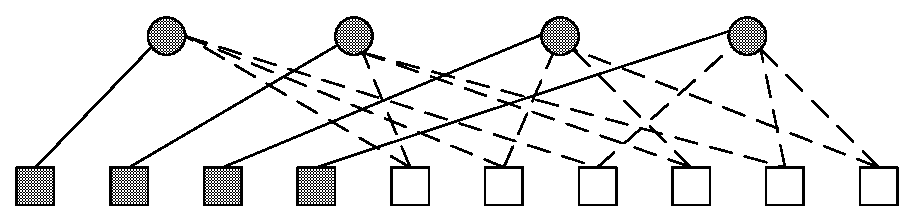
\includegraphics[width=3.0in,height=0.9in]{Drawing11.eps}
\caption{An example of a (4,4) absorbing set} \label{abs44}
\end{figure}


\comment{Moreover, an $(a,b)$ absorbing set can also be
interpreted as follows. For an integer $a$ let $c_a:=c+x_a$, where
$c$ is an arbitrary codeword in the code with the parity check
matrix $H$, and where $x_a$ is a binary vector with non zero
entries in precisely $a$ positions. Let $s_a=Hc_a$, and let $b$ be
the weight of $s_a$. If the weight of $s_a$ strictly increases
when the support of $x_a$ is decreased, the vertex induced
subgraph in $G_H$ induced by the support of $x_a$ and the support
of $s_a$ represents an $(a,b)$ absorbing set.}



We have introduced the notion of absorbing sets to qualitatively
describe the convergent non-codeword state of the message passing
algorithms, when the transmission channel is additive white
gaussian noise (AWGN). In the asymptotic limit given by the bit
flipping algorithm, the configuration described as a fully
absorbing set is stable, since each bit node receives strictly
more messages from the neighboring checks that reinforce its value
than messages that suggest the opposite bit value.

\subsection{Related Work and Existing Concepts}\label{relcon}

The observation that  the low BER/FER performance of finite length
LDPC codes under iterative decoding is guided by non-codewords is
not new. One of the first such attempts to explain these findings
was described in \cite{mackay} where it was recognized that
non-codewords, rather than minimum distance codewords, can attribute
to the error floor. There, the notion of a near-codeword was
introduced. An $(a,b)$ near-codeword refers to a binary string
$\mathbf{s}$ of weight $a$ whose syndrome $\mathbf{s}H^T$ has weight
$b$. A fully absorbing set can be viewed as a near codeword as
defined in \cite{mackay}, though the reverse is not true, since a
near codeword does not necessarily describe a stable configuration.

The trapping sets were introduced in \cite{richardson}  as a part
of the study of error floors of LDPC codes, which pioneered a
simulation-emulation approach. Trapping sets as defined in
\cite{richardson} carry an operational, decoder dependent
definition. In addition, they are defined as a union of all bits
that are not eventually correct, and thus permit a situation in
which the decoder oscillates among a finite number of states.

Stopping sets introduced and studied in detail in \cite{di_stop}
refer to the subgraph of the Tanner graph with the property that
no check node relative to this subgraph has degree 1. These sets
describe stable combinatorial configurations in the context of a
binary erasure channel (BEC), since the decoder halts once it
encounters a stopping set in which all bit nodes were erased. The
stopping sets have been shown to be a very useful tool in
understanding the performance of LDPC codes on erasure channels,
both for finite-length codes \cite{kashyap:03} as well as the
asymptotic behavior of LDPC code ensambles, \cite{orlitsky:05}.
Nevertheless, such analysis cannot be directly applied to an AWGN
channel since the nature of errors is different.

Additional related notions previously introduced in the literature
include pseudo-codewords \cite{wainwrig} and elementary trapping
sets \cite{milenkov}. Note that the pseudo-codewords are defined
in the context of the linear programming based decoding and their
connection with the convergent non-codeword states of the
iterative decoding algorithms though interesting is not yet fully
established. Pseudo-codewords were also studied in \cite{vontobel}
where it was observed that under so-called graph cover decoding,
pseudo-codewords in the covers of the bipartite graph, along with
the actual codewords, compete to be the best estimate produced by
the decoder. Loop calculus method discussed in \cite{chertkov}
provides a way to improve linear programming based decoding once
the so-called critical loop is identified. While for short codes,
as the (155,64) LDPC code discussed in \cite{chertkov}, one loop
may be sufficient to describe a critical state, it would be
interesting to investigate how this concept extends to larger
codes. While \cite{chertkov} uses a search algorithm to find
``bad'' configurations for the (155,64) LDPC code, one could,
based on the structure of the parity check matrix of this code,
analytically describe dominant absorbing sets, and then use these
as a starting point for further analysis. It would be interesting
to further pursue this connection.

Elementary trapping sets are defined as subgraphs in the Tanner
graph in which each check satisfied with respect to this subgraph
has degree 2 and each check  unsatisfied with respect to this
subgraph has degree 1, \cite{milenkov}. \comment{Note that for
example a cycle of length $g$  where $g$ is the girth of the Tanner
graph satisfies the definition of the elementary trapping set.
However, when the bit node degree is large enough, say larger than
4, the message passing
 decoder will not converge to such a configuration since there will
be strictly more unsatisfied than satisfied checks to pull it away
from this configuration.} In a loose sense, one may view absorbing
sets as consisting of a union of elementary trapping sets in some
cases.

\chapter[Absorbing Sets of Array-based LDPC Codes]{Absorbing Sets of Array-based LDPC
Codes}\label{arrayabs}

In this chapter we provide a detailed analysis of the  minimal
absorbing sets and minimal fully absorbing sets of the high rate
array-based LDPC codes. In particular we will show that for
$\gamma=2$ the minimal (fully) absorbing sets are in fact minimum
distance codewords, whereas, for $\gamma=3$ and $\gamma=4$, minimal
(fully) absorbing sets are in fact strictly smaller that the minimum
distance of the code.


\section{Array-based LDPC codes}
% no \PARstart
%This demo file is intended to serve as a ``starter file"
%for IEEE conference papers produced under \LaTeX\ using IEEEtran.cls version
%1.6b and later.

% May all your publication endeavors be successful.

%\hfill mds

%\hfill November 18, 2002

Array based LDPC codes \cite{fan} are regular LDPC codes
parameterized by a pair of integers $(p,\gamma)$, such that $\gamma
\leq p$, and $p$ is an odd prime, with a parity check matrix
$H_{p,\gamma}$ given by
\begin{equation}\label{eq:1}
H_{p,\gamma}=\left[\begin{array}{ccccc}
I & I & I & \ldots & I\\
I & \sigma & \sigma^2 & \ldots &\sigma^{p-1}\\
I & \sigma^2 & \sigma^4 & \ldots &\sigma^{2(p-1)}\\
\vdots & \vdots & \vdots & \ldots & \vdots \\
I & \sigma^{\gamma-1} & \sigma^{(\gamma-1)2} & \ldots &\sigma^{(\gamma-1)(p-1)}\\
\end{array}
\right]
\end{equation}\normalsize
where $\sigma$ denotes a $p \times p$ permutation matrix of the
form \small
\begin{equation}
\sigma=\left[\begin{array}{ccccc}
0 & 0 & \ldots & 0 & 1\\
1 & 0 & \ldots & 0 & 0\\
0 & 1 & \ldots & 0 & 0\\
\vdots & \vdots & \ldots & \vdots & \vdots\\
0 & 0 & \ldots & 1 & 0\\
\end{array}
\right].
\end{equation}
\normalsize We use $C_{p,\gamma}$ to denote the binary linear code
with parity check matrix of the form \eqref{eq:1}. The rate of
this code is $R=1-\frac{\gamma p-\gamma+1}{p^2}$,
\cite{mittel:02}.

As first demonstrated by Fan \cite{fan}, array-based LDPC codes
have very good performance. They have been proposed for a number
of applications, including digital subscriber lines \cite{ibm:02}
and magnetic recording  \cite{vasic:05}.




In our earlier experimental work \cite{zhang06} we have observed
that certain structures in the Tanner graph of the parity check
matrix of the code are the limiting factor in the iterative decoding
of several structured LDPC codes, including array-based codes.
Motivated by the empirical findings, we introduced this object,
which we call an \emph{absorbing set}. The formal definition of
absorbing sets is given in Section~\ref{absformal}. Here we study
them in detail for array-based LDPC codes $C_{p,\gamma}$ for
$\gamma=2,3,4$, for the standard parity check matrix $H_{p,\gamma}$.

%We now formally introduce the notion of an absorbing set useful in
%studying the limiting behavior of the message passing algorithm in
%the very low BER region.


\section{Theoretical Results}\label{theo1}

Our goal is to describe minimal absorbing sets and minimal fully
absorbing sets $(a,b)$ of the Tanner graph of the parity check
matrix $H_{p,\gamma}$, for $\gamma =2,3,4$, where the minimality
refers to the smallest possible $a$, and where $b$ is the smallest
possible for the given $a$.

We use the following notation throughout this chapter. Recall that
$H_{p,\gamma}$ is a $\gamma p \times p^2$ matrix of 0's and 1's. It
is convenient to view $H_{p,\gamma}$ as a two-dimensional array of
component $p \times p$ submatrices with the rows $i$ in the range $0
\leq i \leq \gamma-1$ (also referred to as row groups) and the
columns $j$ in the range $0 \leq j \leq p-1$ (also referred to as
column groups). Each column of $H_{p,\gamma}$ is uniquely described
by a pair $(j,k)$ where $j$ denotes the column index of the
submatrix this column belongs to, and $k$, $0 \leq k \leq p-1$
denotes the index of this column within the submatrix.

\begin{figure}
\center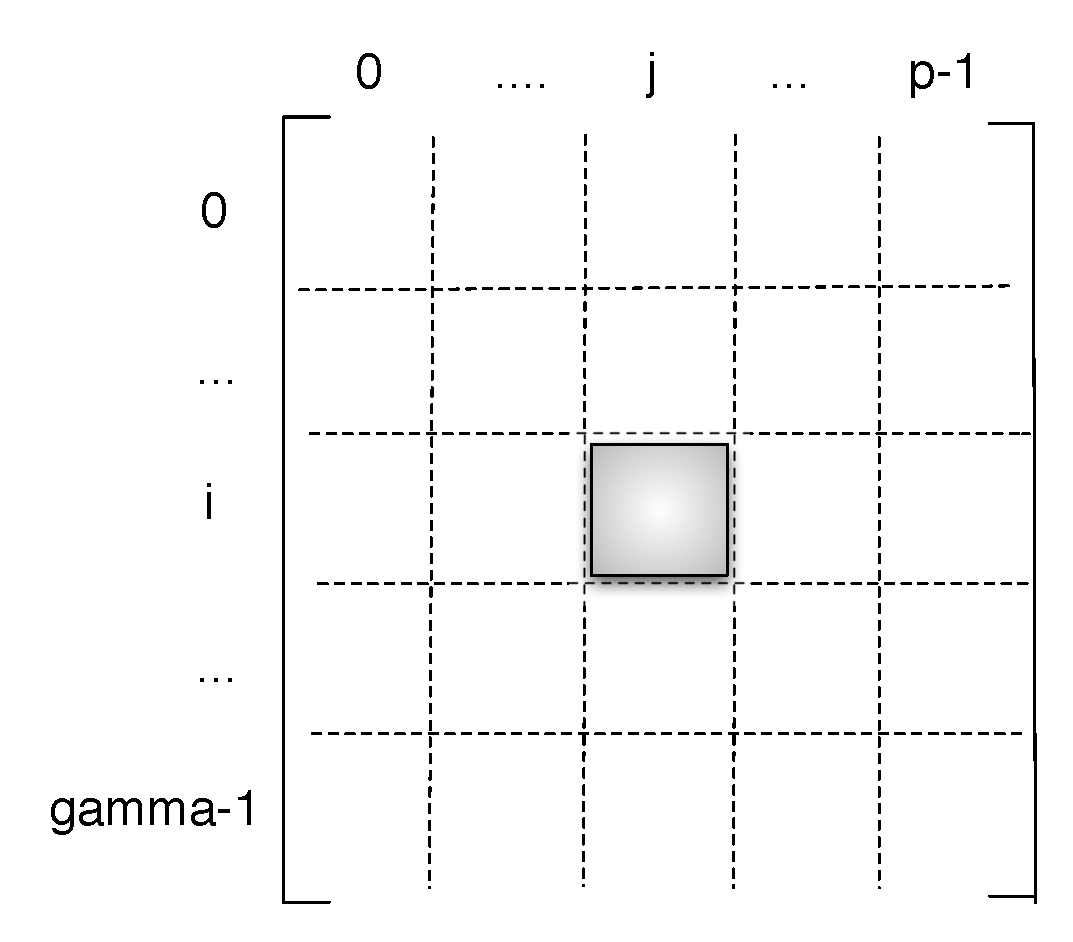
\includegraphics[width=2.8in,height=1.8in]{matrix1.eps}
\\
\hspace{0.65in}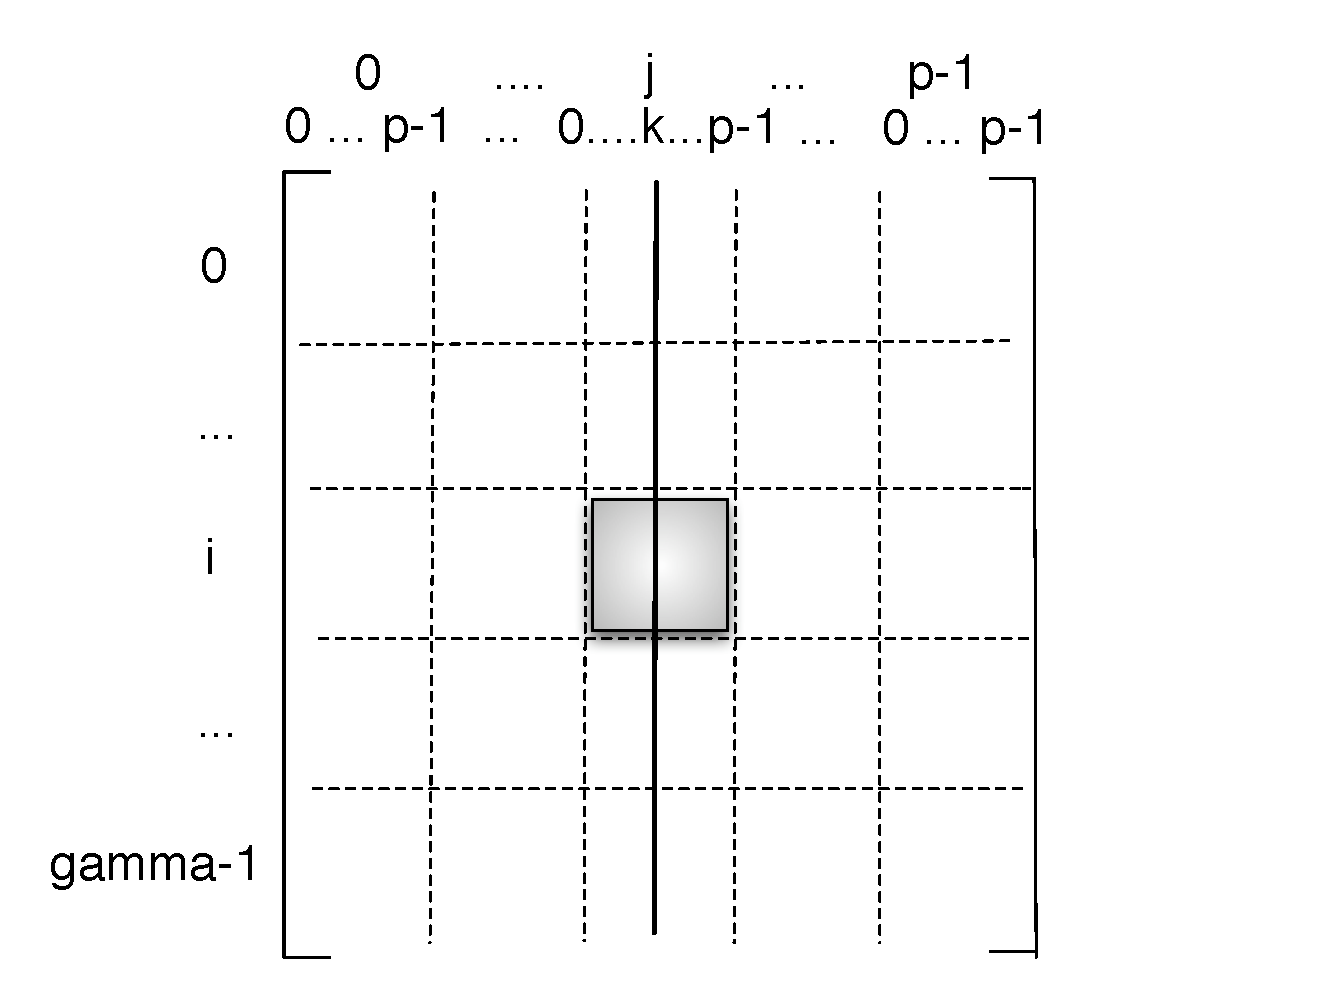
\includegraphics[width=3.4in,height=2.0in]{matrix2.eps}
\caption{Illustration of the notation (a) Row and column groups in
$H_{p,\gamma}$(b) $(j,k)$ column label. Shaded area corresponds to
the submatrix $\sigma^{ij}$.} \label{fig62}
\end{figure}
%, corresponding to the column-wise index in $H_{p,\gamma}$, and
%denoted the column group $j$. Likewise let $i$ in the interval $0
%\leq i \leq \gamma-1$ be the row-wise index in $H_{p,\gamma}$ and
%denoted the row group (or the label) $i$.

Let $G_{p,\gamma}$ be the Tanner graph associated with
$H_{p,\gamma}$, so bit nodes and check nodes in $G_{p,\gamma}$
represent columns and rows in $H_{p,\gamma}$, respectively. In
$G_{p,\gamma}$ bit nodes have degree $\gamma$ and check nodes have
degree $p$. There is a total of $p^2$ bit nodes and $\gamma p$ check
nodes. Each bit node in $G_{p,\gamma}$ receives the unique label
$(j,k)$ that describes the corresponding column of $H_{p,\gamma}$.
Each check node in $G_{p,\gamma}$ receives a label $i$ if
 the corresponding row of $H_{p,\gamma}$ belongs to the row group
$i$. Multiple bit nodes can have the same $j$ or $k$ label, but not
both. Multiple check nodes can have the same $i$ label.

We note that the structure of the parity check matrix imposes the
following conditions on the neighboring bit nodes and check nodes:

\textit{Bit Consistency:} For a bit node, all its incident check
nodes, labelled $i_{s_1}$ through $i_{s_\gamma}$ must have distinct
labels, i.e. these check nodes are in distinct row groups.

\textit{Check Consistency:} All bit nodes, say $(j_{1},k_{1})$
through $(j_{p},k_{p})$, participating in the same check node must
have distinct $j_\ell$ values, i.e. they are all in distinct column
groups.

Both conditions follow from the fact that the parity check matrix
$H_{p,\gamma}$ of $C_{p,\gamma}$ consists of a 2-dimensional array
of permutation matrices of equal size.\hfill$\blacksquare$

We begin with elementary lemmas that play a central role throughout
this chapter.

\comment{\begin{lemma}\textit{Pattern consistency:}Consider the
matrices $\sigma^{ij_1}$ and $\sigma^{ij_2}$ in the same row group
of $H_{p,\gamma}$, \eqref{eq:1}. Suppose the matrix $\sigma^{ij_1}$
has a non-zero entry in position $(r,k_1)$ (i.e. row $r$ and column
$k_1$) for a given $k_1$. Then, the unique non-zero entry in the row
$r$ of $\sigma^{ij_2}$ is in position $(r,k_2)$ such that
\begin{eqnarray}\label{cong}
k_1+ij_1 \equiv k_2+ij_2 \mod p~.
\end{eqnarray}\end{lemma}

\noindent \textit{Proof:} The congruential constraint
in~\eqref{cong} is derived from the following. Assume that the
columns of $\sigma^{ij}$ are indexed with $0$ through $p-1$. Recall
that $\sigma$ has `1' in the first row in column indexed $p-1$ (last
column), and that each subsequent row has `1' in a position that is
a cyclic shift to the right of the position of `1' in the previous
row. Multiplying $\sigma^{ij}$ with $\sigma$ cyclically shifts the
entries by one position to the left. Thus, $\sigma^{ij_1}$ has `1'
in the first row in column $(p-ij_1) \mod p$, and has `1' in some
row $r$ in the column $k_1 \equiv p-ij_1+r-1 \mod p$.  Likewise,
$\sigma^{ij_2}$ has `1' in this row $r$ in the column indexed $k_2
\equiv p-ij_2+r-1 \mod p$. Equating these expressions in terms of
$r$, the statement in \eqref{cong} follows.\hfill$\blacksquare$

Note that the expression of the type~\eqref{cong} relates the
coordinates of the bit nodes $(j_1,k_1)$ and $(j_2,k_2)$ that both
participate in a check in the row group $i$. We will refer to the
constraint of the type described in~\eqref{cong} as the parity check
consistency constraint.} % end comment

\begin{lemma}\label{patternlemma}(\textit{Pattern Consistency}): The $(r,k)$ entry of $\sigma^{i}$
is 1 iff $r-k \equiv i \mod p$.
\end{lemma}
\begin{corollary}\label{patterncor}(\textit{Pattern Consistency}): Let
$\sigma^{ij_1}$ and $\sigma^{ij_2}$ be in the same row group of
$H_{p,\gamma}$. If the entry $(r,k_1)$ of $\sigma^{ij_1}$ is
non-zero, then so is the entry $(r,k_2)$ of $\sigma^{ij_2}$ where
$k_1+ij_1 \equiv k_2+ij_2 \equiv r \mod p$.
\end{corollary}

We will refer to the constraints of the type described in both
Lemma~\ref{patternlemma} and Corollary~\ref{patterncor} as
\textit{pattern consistency} constraints.

\begin{lemma}\label{cyclelemma}(\textit{Cycle consistency:}) Consider a cycle in $G_{p,\gamma}$ of
length $2t$, involving $t$ bit nodes, with labels $(j_1,k_1)$
through $(j_t,k_t)$ and $t$ check nodes, with labels $i_1$ through
$i_t$, such that bit nodes $(j_1,k_1)$ and $(j_2,k_2)$ participate
in the check labelled $i_1$, $(j_2,k_2)$ and $(j_3,k_3)$ participate
in the check labelled $i_2$, and so on, until check labelled $i_t$
in which $(j_t,k_t)$ and $(j_1,k_1)$ participate. Then
\begin{equation}\label{cycles}
i_1(j_2-j_1)+i_2(j_3-j_2)+\dots+i_{t-2}(j_{t-1}-j_{t-2})+i_{t-1}(j_t-j_{t-1})+
i_t(j_1-j_t) \equiv 0 \mod p.
\end{equation}
\end{lemma}
\noindent \textit{Proof:} The pattern consistency constraints of
Corollary~\ref{patterncor} give:
\begin{equation}\begin{array}{cccc}
k_1+i_1j_1 &\equiv&k_2+i_1j_2 & \mod p, \\
k_2+i_2j_2 &\equiv&k_3+i_2j_3 & \mod p, \\
{} & \vdots & {}\\
k_{t-1}+i_{t-1}j_{t-1} &\equiv&k_t+i_{t-1}j_t & \mod p, \\
k_t+i_tj_t &\equiv&k_1+i_tj_1 & \mod p.
\end{array}\end{equation}

Expand $k_1-k_2$ into
$(k_1-k_t)-(k_{t-1}-k_t)-(k_{t-2}-k_{t-1})-\dots-(k_2-k_3)$.
Hence,
\begin{equation}
i_1(j_2-j_1) \equiv
i_t(j_t-j_1)-i_{t-1}(j_t-j_{t-1})-i_{t-2}(j_{t-1}-j_{t-2})-\dots-i_2(j_3-j_2)
\mod p.
\end{equation} By rearranging the terms,~\eqref{cycles} follows.\hfill$\blacksquare$

Constraints of the type~\eqref{cycles} will subsequently be referred
to as cycle consistency constraints.

%We say that the number $Q$ of particular absorbing sets  grows as
%$\Theta(n^l)$ if $cn^l \leq Q \leq c'n^l$, for some constants $c$
%and $c'$.

Our main results can be summarized as follows: Let $G_{p,\gamma}$
be the Tanner graph associated with the parity check matrix
$H_{p,\gamma}$ of the array-based LDPC code $C_{p,\gamma}$.
\begin{theorem}\label{theo1}\emph{Minimality}

(a) For the $G_{p,2}$ family, all minimal absorbing sets are
minimal fully absorbing sets and are of size $(4,0)$.

(b) For the $G_{p,3}$ family, the minimal absorbing sets are of
size $(3,3)$, and the minimal fully absorbing sets are of size
$(4,2)$.

(c) For the $G_{p,4}$ family, and for $p>19$, all minimal absorbing
sets are fully minimal absorbing sets, and are of size
$(6,4)$.\hfill$\blacksquare$
\end{theorem}
\begin{theorem}\label{theo2}\emph{Scaling}

(a) Suppose $\gamma=2$ and $p>3$. The number of minimal (fully)
absorbing sets in $G_{p,\gamma}$ grows with block length $n$ (Recall
that the blocklength $n=p^2$, given by the number of columns in
$H_{p,\gamma}$) as $\Theta(n^{2})$.

(b) For $\gamma=3$ and for all blocklengths $n>3^2$ the number of
minimal absorbing sets as well as the number of minimal fully
absorbing sets in $H_{p,\gamma}$ is $\Theta(n^{3/2})$.

(c) For $\gamma=4$ and for all blocklengths $n>19^2$ the number of
minimal absorbing sets as well as the number of minimal fully
absorbing sets in $H_{p,\gamma}$ is $\Theta(n^{3/2})$.
\hfill$\blacksquare$
\end{theorem}




Here we say that the number $Q$ of particular absorbing sets  grows
as $\Theta(n^l)$ if $cn^l \leq Q \leq c'n^l$, for some constants $c$
and $c'$.

The following three subsections provide proofs of these claims,
where we separately treat each of the values of $\gamma$. While our
results provide a precise count of the minimal (fully) absorbing
sets, the main message is regarding the cardinality scaling is that
of Theorem~\ref{theo2}.


Note that Theorem \ref{theo1}(a) implies that for $\gamma=2$ the
smallest (fully) absorbing sets are in fact the minimum distance
codewords. This is in contrast to the results in Theorem
\ref{theo1}(b) for $\gamma=3$ and \ref{theo1}(c) for $\gamma=4$ for
which we show the existence of (fully) absorbing sets strictly
smaller than the minimum distance of the code. In particular, for
$\gamma=3$, the minimum distance is 6 \cite{helles},
\cite{mittel:02}, and for $\gamma=4$ and $p>7$ the minimum distance
is between $8$ and $10$, \cite{helles},\cite{mittel:02}. The minimal
absorbing sets and minimal fully absorbing sets  are for both
$\gamma=3$ and $\gamma=4$ and $p$ large enough strictly smaller than
the minimum distance of the code.
\vspace{-0.00in}\subsection{Absorbing sets of
$H_{p,2}$}\label{theo12}

%Even though the $C_{p,2}$ code may not be of much practical
%interest due to the small minimum distance we include its analysis
%for completeness' sake.
The code $C_{\gamma,2}$ has uniform bit degree 2, and is thus a
cycle code. Even though such codes are known to be poor
\cite{peterson}, we include the analysis for the sake of
completeness.
%\begin{lemma}\label{Lemma02} The minimal absorbing set for $C_{p,2}$
%is if of dimension $(4,0)$.
%\end{lemma}
We start by proving the statement in Theorem~\ref{theo1}(a).
%\noindent \textit{Proof:}
\comment{ It follows from the definition of the absorbing set that
all $a$ bit nodes must be connected to satisfied checks with
respect to the subgraph induced by these bit nodes. The minimal
absorbing set thus corresponds to the support of a minimum weight
codeword. Since $\gamma=2$, Massey's theorem \cite{lincostel}
guarantees that $d_{min} \geq 4$. We first show that the smallest
cycle in this code is of length 8. We note that a cycle of length
4 cannot exist, as it would imply the existence of $\sigma^{j_1}$
and $\sigma^{j_2}$, for $0 \leq j_1, j_2 \leq p-1$ and $j_1 \neq
j_2$ that contain the same row. (Recall that the top row of
$H_{p,\gamma}$ consists of a row of identity matrices.) This
set-up is impossible by the code construction. For the same
reason, nor does there exist a cycle of length 6. We now show that
$a=4$ and these bit nodes complete an 8-cycle with their shared
check nodes. }

Let $G_{p,2}=(V,F,E)$ denote the Tanner graph of $H_{p,2}$. Let
$D$ be an $(a,b)$ absorbing set in $G_{p,2}$. Each bit node in $D$
has degree $2$ in $G_{p,2}$ and is required to have strictly more
neighbors in $\mathcal{E}(D)$ than in $\mathcal{O}(D)$. This
implies that $\mathcal{O}(D)$ is empty. The absorbing set is of
type $(a,0)$. It is thus a fully absorbing set, and is in fact a
codeword.

Since the matrix $H_{p,2}$ has the top row consisting of identity
matrices, the codewords of $C_{p,2}$ are of even weight. Moreover,
since the bottom row of $H_{p,2}$ consists of distinct component
submatrices, no two columns of $H_{p,2}$ sum to zero. Therefore
$a>2$ and even and there are no cycles of length 4 in this code.

We now consider $a = 4$. Let $(j_1,k_1)$, $(j_2,k_2)$, $(j_3,k_3)$
and $(j_4,k_4)$ be the bit nodes participating in a candidate
$(4,0)$ absorbing set. These nodes must necessarily be arranged as
in Figure~\ref{Fig03}.%, since there are no cycles of length 4 in
%this code \cite{fan}.
%\begin{figure}
%\center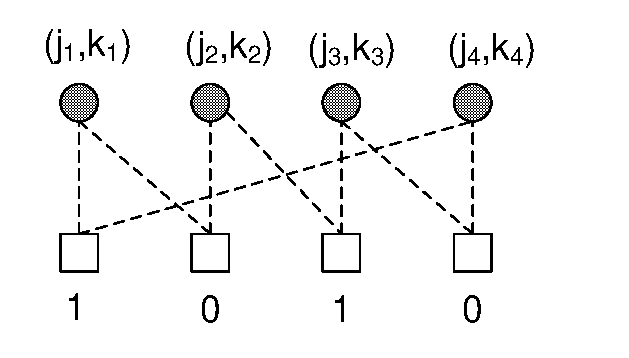
\includegraphics[width=2.75in,height=1.4in]{fig03.eps}
%\caption{(Labelled) candidate (4,0) absorbing set}\label{Fig03}
%\end{figure}
\begin{figure}
\center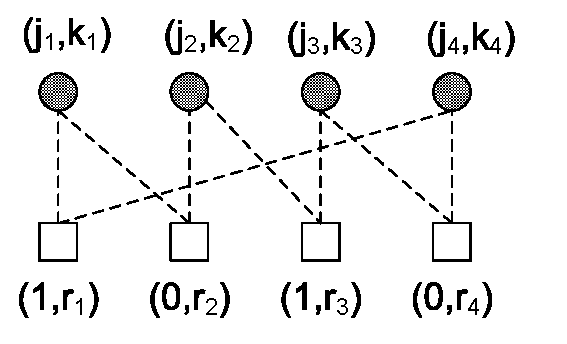
\includegraphics[width=2.75in,height=1.4in]{Visio-fig03z.eps}%{fig03.eps}
\caption{(Labelled) candidate (4,0) absorbing set}\label{Fig03}
\end{figure}
%By the bit consistency condition, all the bit nodes that share
%a check node have different first indices. We may thus assume that
%$(j_1,k_1)$ and $(j_2,k_2)$ share a check in the row group $0$, as
%do $(j_3,k_3)$ and $(j_4,k_4)$, and that $(j_2,k_2)$ and
%$(j_3,k_3)$ share a check in the row group $1$, as do $(j_4,k_4)$
%and $(j_1,k_1)$, as shown in Figure \ref{Fig03}.
%Note that the bits in this absorbing set along with their shared
%checks constitute a cycle of length 8. Using
%Lemma~\ref{cyclelemma} it follows that
%\begin{equation}\label{eq1}
%p\ell=j_3-j_2+j_1-j_4,
%\end{equation}
%for some integer $\ell$.

 \comment{Consider the matrix $M$,
\begin{equation}\label{matrixM}
M=(\sigma^{0j_1})^T(\sigma^{0j_2})(\sigma^{1j_2})^T(\sigma^{1j_3})(\sigma^{0j_3})^T(\sigma^{0j_4})(\sigma^{1j_4})^T(\sigma^{1j_1})~.
\end{equation}

By traversing the cycle in Figure~\ref{Fig03}, starting at the bit
node $(j_1,k_1)$ and then going into its neighboring check with
the label '0', we require that the matrix $M$ given in
\ref{matrixM} is an identity matrix. Since $M$ is itself a power
of $\sigma$, it is necessary that $M=\sigma^{p\ell}$, for some
$\ell$, where $\ell$ is an integer.

Moreover, since each component submatrix is a permutation matrix,
\begin{equation}\label{eq1a}
(\sigma^{\ell})^T=(\sigma^{\ell})^{-1} \end{equation} it further
follows that
\begin{equation}\label{eq1}
p\ell=j_3-j_2+j_1-j_4.
\end{equation}}

\comment{One solution to the last equation is $\ell = 0$, and
$j_1=1, j_3=p-1, j_2=2, j_4=p-2$. Since $(j_1,k_1)$ and
$(j_2,k_2)$ share a check in the row group $0$, it follows that
$k_1=k_2$, and likewise $k_3=k_4$. Since the column $k_2$ of
$\sigma^{j_2}$ and column $k_3$ of $\sigma^{j_3}$ have a non-zero
entry in the same row, it follows that
\begin{eqnarray*}
k_2+j_2 &\equiv & k_3+j_3 \mod p.
\end{eqnarray*}

Thus, the indices of the bit nodes participating in one such
absorbing set are $(j_1,k_1)$, $(j_2,k_1)$, $(j_3,[k_1-p+3]_p)$,
and $(j_4,[k_1-p+3]_p,)$, for $k_1$ chosen arbitrary in the
residue set$\mod p$, and where $[x]_p$ here and in the remainder
denotes a residue congruent to $x\mod p$.\hfill$\blacksquare$}

%It can be checked that for $\gamma=2$ the indicator function of
%every absorbing set is a codeword.
%\begin{lemma} The total number of $(4,0)$ absorbing sets in $C_{p,2}$ is XXXXX.
%\end{lemma}
%\noindent \textit{Proof:} It suffices to consider $l=-1,0,1$ in
%\ref{eq1}). First, for $l=0$ there are \hfill$\blacksquare$

The following result proves Theorem \ref{theo1}(a).
\begin{lemma}\label{lemma40} There is a total of $p^2(p-1)^2$ $(4,0)$ (fully) absorbing sets in
the code described by $H_{p,2}$.
\end{lemma}
\comment{\noindent \textit{Proof:} Since $j_3-j_3+j_1-j_4 \in
[-2(p-1), 2(p-1)]$ and $2(p-1)<2p$, it suffices to consider
$\ell=1,0,-1$ in (\ref{eq1}). Recall that $j_1,j_2,j_3,j_4$ in
\eqref{eq1} all belong to the set $\{0,\dots,p-1\}$.

First, for $\ell=1$, note that since $j_1+j_3$ is at most $2p-2$,
 $j_2+j_4$ is at most $p-2$. For each integer $s$ such that $0 \leq s \leq p-2$ there are
$(s+1)$ ways of assigning values to $j_2$ and $j_4$ to make
$j_2+j_4=s$. For each such $s$, there are $p-s-1$ ways of assigning
values to $j_1$ and $j_3$ to make $j_1+j_3=p+s$. Summing over all
choices of $s$ yields
\begin{equation}\label{sum401}\sum_{s=0}^{p-2}
(s+1)(p-s-1)=p(p-1)(p+1)/6\end{equation} as the total number of ways
of assigning values to $(j_1,j_2,j_3,j_4)$. By symmetry, for
$\ell=-1$ there are also $p(p-1)(p+1)/6$ ways of assigning values to
$(j_1,j_2,j_3,j_4)$.

For $\ell=0$, the sum $j_1+j_3$ is at most $2p-2$. For each $s$,
$0 \leq s \leq p-1$, there are $s+1$ ways of expressing $s$ as a
sum of an ordered pair $(j_1,j_3)$. For each $s$, $p-1 \leq s \leq
2p-2$, there are $2p-2-s+1$ ways of expressing it as a sum of an
ordered pair $(j_1,j_3)$, which is thus the same as the number of
assignments for $2p-2-s$.

It now suffices to consider $s$ where $0 \leq s \leq p-1$. Since we
are dealing with the $j_1+j_3 = j_2+j_4$ case, the numerical
assignment that makes $j_1=j_3 (j_4)$ or  $j_2=j_3 (j_4)$ needs to
be excluded by the check consistency condition.  For $s$ odd and $0
\leq s \leq p-1$, each of these $s+1$ ordered pairs can be assigned
to $(j_1,j_3)$, and for each such assignment, $s-1$ ordered pairs
can be assigned to $(j_2,j_4)$ (the two excluded cases are the ones
involving the assigned values to $j_1$ and $j_3$). For $s$ even, for
$s$ assignments out of possible $s+1$ (excluding the pair
$(s/2,s/2)$) of $(j_1,j_3)$, $s-1$ ordered pairs can be assigned to
$(j_2,j_4)$. For the pair $(s/2,s/2)$ assigned to $(j_1,j_3)$, there
are $s$ available assignments for $(j_2,j_4)$. The total number of
assignments for $l=0$ is
\begin{eqnarray}\label{sum402} 2\sum_{s=1,s \text{ odd}}^{p-2} (s+1)(s-1) + 2\sum_{s=2,s
\text{ even}}^{p-3} \left[s(s-1)+s\right] +
\left[(p-1)(p-2)+(p-1)\right] = 2p(p-1)(p-2)/3~.\end{eqnarray}

By summing~\eqref{sum402} with twice the expression
in~\eqref{sum401}, the total number of assignments for
$(j_1,j_2,j_3,j_4)$ is then $p(p-1)^2$. Since the column $k_1$ of
$\sigma^{1j_1}$ and the column $k_4$ of $\sigma^{1j_4}$ have a
non-zero entry in the same row, it follows by the parity check
consistency constraint
\begin{equation*}
k_1+j_1 \equiv k_4+j_4 \mod p~.
\end{equation*}
Likewise,
\begin{equation*}\begin{array}{cccc}
k_2+j_2 &\equiv &k_3+j_3,  \mod p\\
k_1 &\equiv &k_2 \mod p~, \text{ and}\\
 k_3 &\equiv &k_4\mod p~.
\end{array}\end{equation*}

Therefore, once the values of  $(j_1,j_2,j_3,j_4)$ are selected,
$k_1$ can be chosen in $p$ ways, and for each such assignment, the
values of $k_2$, $k_3$, and $k_4$, are then uniquely determined.
Hence, there are $p^2(p-1)^2$ different $(4,0)$ (fully) absorbing
sets.\hfill$\blacksquare$} %% end comment

\noindent \textit{Proof:} The bit consistency conditions are
automatically satisfied by the numbering of the row groups in
Figure~\ref{Fig03}. The check consistency constraints give:
\begin{equation}\begin{array}{ccc}j_1 \neq j_4&{}\\
j_1 \neq j_2 &{}\\
j_2 \neq j_3 &{}\\
j_3 \neq j_4&~.\end{array}
\end{equation}

The pattern consistency constraints of Corollary~\ref{patterncor}
give:
\begin{equation}\begin{array}{ccc} k_1 = k_2 &{}\\
k_3 = k_4 &{}\\
k_2+j_2 \equiv  k_3+ j_3 & \mod p\\
k_4+j_4 \equiv k_1 +j_1 & \mod p.\end{array}
\end{equation}

There are $p$ ways of choosing $k_2$, which also determines $k_1$.
Since $j_2 \neq j_3$, we must have $k_3 \neq k_2$, so we have
$(p-1)$ ways of choosing $k_3$, which also determines $k_4$.  We
then have $p$ ways of choosing $j_2$, which also determines $j_3$.
Since $j_1 \neq j_2$, we have $(p-1)$ ways of choosing $j_1$, which
also determines $j_4$. To verify that every one of these choices
satisfies all the equations it only remains to verify that $j_3 \neq
j_4$. This holds because
\begin{equation}
j_3 -j_4 \equiv (k_2-k_3+j_2)-(k_1-k_4+j_1) \equiv j_2 -j_1 \neq 0
\mod p~.
\end{equation}

Now, for any choice of row group labels for the checks, and column
labels for the bits that satisfy the bit and check consistency
constraints and the pattern consistency constraints of
Corollary~\ref{patterncor} there is a unique way to choose the row
index in the individual row groups so that the pattern consistency
constraint of Lemma~\ref{patternlemma} are satisfied. This completes
the proof of Lemma~\ref{lemma40}.\hfill$\blacksquare$


 Theorem \ref{theo2}(a) is now a consequence of
\begin{corollary} The number of $(4,0)$ (fully) absorbing sets for
the code described by $H_{p,2}$ is $\Theta(n^{2})$, where $n$ is
the codeword length.
\end{corollary}
\noindent \textit{Proof:} Follows immediately from
Lemma~\ref{lemma40} and $n=p^2$.\hfill$\blacksquare$
% end of the comment

Note that $(4,0)$ absorbing sets are actually codewords, so  the
cycle code is dominated by low weight codewords. We now consider
$\gamma
> 2$, which leads to more interesting results. In particular, our results establish the
existence of minimal absorbing sets and minimal fully absorbing
sets, for which the number of bit nodes $a$ is \emph{strictly
smaller} than the minimum distance $d_{min}$ of the code.

\subsection{Absorbing sets of $H_{p,3}$}\label{theo12}

%\begin{lemma}\label{Lem1} The minimal absorbing set for $C_{p,3}$
%is a $(3,3)$ absorbing set.
%\end{lemma}
%\noindent \textit{Proof:}
We now turn to the proof of Theorem~\ref{theo1}(b), concerning the
sizes and numbers of minimal absorbing sets in $H_{p,3}$.

\comment{First observe that if there were to exist an unsatisfied
check node connected to three bit nodes participating in one such
absorbing set, there would necessarily exist a satisfied check
node connected to two of these three bit nodes. This however
violates the girth condition of the code. It is thus necessary
that all three bit nodes have a different unsatisfied check,
implying $b=3$. Moreover, these $a=3$ bits along with their shared
satisfied checks create a length 6 cycle.}

Let $G_{p,3}=(V,F,E)$ denote the Tanner graph of $H_{p,3}$. Let
$D$ be an $(a,b)$ absorbing set in $G_{p,3}$. Each bit node in $D$
has degree $3$ in $G_{p,3}$ and is required to have strictly more
neighbors in $\mathcal{E}(D)$ than in $\mathcal{O}(D)$.

\begin{figure}
\center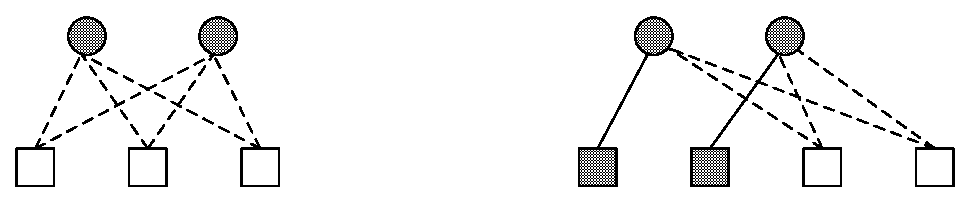
\includegraphics[width=3.45in,height=0.8in]{fig07.eps}
\caption{Candidate (2,b) absorbing sets}\label{Fig07}
\end{figure}
Suppose $a=2$. In $G_{p,3}$ an even number of edges from $D$
terminates in $\mathcal{E}(D)$. Thus either $b=0$ or $b=2$. These
correspond to the situations in Figure \ref{Fig07}. In either case
there would be a cycle of length 4 in $G_{p,3}$, which is false
\cite{fan}. Thus $a\geq 3$.

Suppose $a=3$. In $G_{p,3}$ an even number of edges from $D$
terminates in $\mathcal{E}(D)$. Thus either $b=1$ or $b=3$. Suppose
$b=1$. This must correspond to the left form in Figure \ref{Fig06},
or the right form in Figure \ref{Fig06},
%\begin{figure}
%\center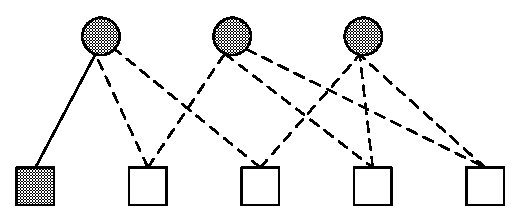
\includegraphics[width=1.9in,height=0.9in]{fig06a.eps}
%\caption{Candidate (3,1) absorbing set}\label{Fig06}
%\end{figure}
\begin{figure}
\center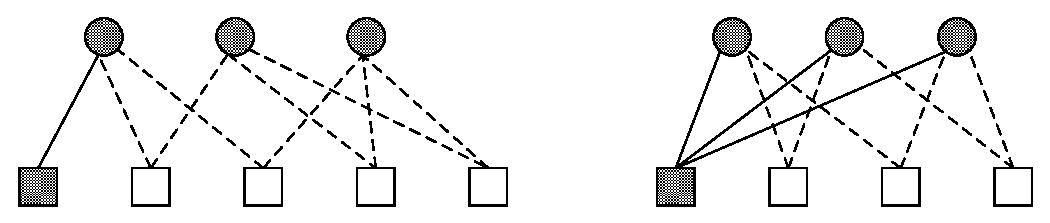
\includegraphics[width=3.1in,height=0.9in]{Visio-fig05z.eps}%{fig06a.eps}
\caption{Candidate (3,1) absorbing sets}\label{Fig06}
\end{figure}
which again involves a cycle of length 4 in $G_{p,3}$, a
contradiction, \cite{fan}.

The remaining case with $a=3$ is $b=3$. In this case, each bit node
in $D$ would then connect to exactly one check node in
$\mathcal{O}(D)$ implying the unlabelled form of Figure \ref{Fig05}.
%\begin{figure}
%\vspace{0.1in}\hspace{0.4in}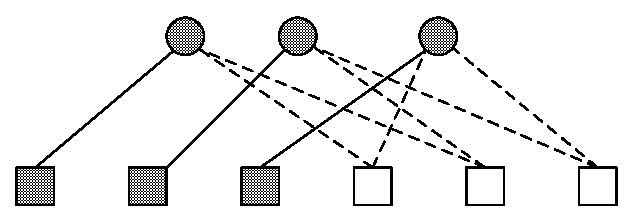
\includegraphics[width=2.5in,height=0.9in]{fig04.eps}
%\caption{Candidate (3,3) absorbing set}\label{Fig04}
%\end{figure}
Note that there is a cycle of length 6. Suppose that these $3$ bit
nodes are indexed as $(j_1,k_1)$, $(j_2,k_2)$ and $(j_3,k_3)$,
respectively, where $j_1,j_2$ and $j_3$ are distinct (by the check
consistency) and $0 \leq j_1, j_2, j_3 \leq p-1$. Without loss of
generality assume that $(j_1,k_1)$ and $(j_2,k_2)$ share a check in
the row group $i_1$, $(j_2,k_2)$ and $(j_3,k_3)$ share a check in
the row group $i_2$, and that $(j_1,k_1)$ and $(j_3,k_3)$ share a
check in the row group $i_3$, where $i_1,i_2,i_3 \in \{0,1,2\}$ and
are distinct by the bit consistency condition. We may assume without
loss of generality that $i_1=0$, $i_2=1$ and $i_3=2$. Note that the
bit consistency constraints force the values of $i_4,i_5$ and $i_6$
to be as given in Figure \ref{Fig05}.

In the remainder of the discussion we will first prove the
existence of a $(3,3)$ absorbing set. We will then show that these
$(3,3)$ absorbing sets are not fully absorbing sets. This result
will in turn imply the existence of $(4,2)$ fully absorbing sets,
which are thus minimal fully absorbing sets for $\gamma=3$.

%\begin{figure}
%\center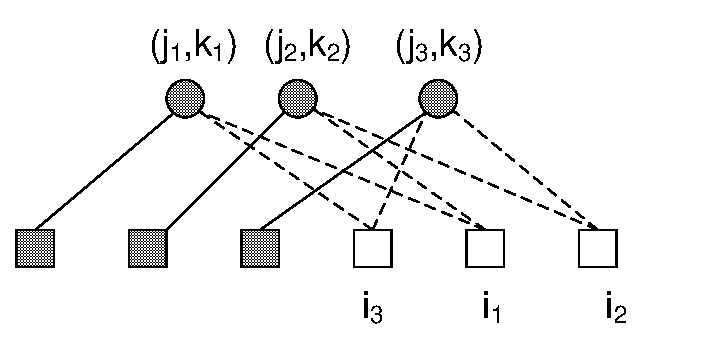
\includegraphics[width=2.7in,height=1.35in]{fig05a.ps}
%\caption{(Labelled) candidate (3,3) absorbing set}\label{Fig05}
%\end{figure}
\begin{figure}
\center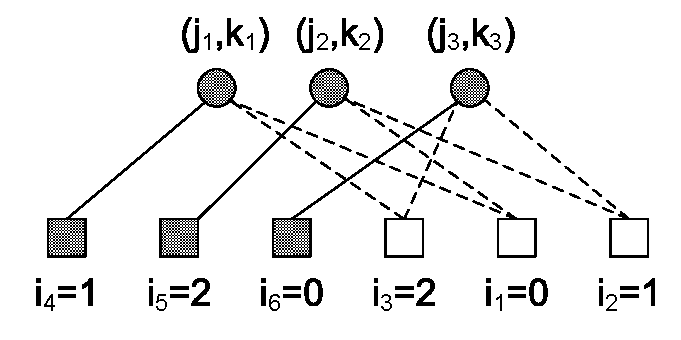
\includegraphics[width=2.8in,height=1.25in]{Visio-fig06z.eps}%{fig05a.ps}
\caption{(Labelled) candidate (3,3) absorbing set}\label{Fig05}
\end{figure}

\comment{Consider the length-6 cycle involving bit nodes
$(j_1,k_1)$, $(j_2,k_2)$, and $(j_3,k_3)$ as shown in
Figure~\ref{Fig05}. Using the cycle consistency condition  it
follows that
\begin{equation}\label{eqpl}
p\ell=i_1(j_2-j_1)+i_2(j_3-j_2)+i_3(j_1-j_3).\end{equation}}%%% end comment

\comment{By tracing the cycle in \ref{Fig05} we obtain that the
matrix $M_1$, where $M_1$ given by
\begin{equation}
M_1=(\sigma^{i_1j_1})^T(\sigma^{i_1j_2})(\sigma^{i_2j_2})^T(\sigma^{i_2j_3})(\sigma^{i_3j_3})^T(\sigma^{i_3j_1}),
\end{equation}
is an identity. Since $M_1$ has a non-zero entry on the main
diagonal, and is itself a power of $\sigma$, it is necessary that
$M_1=\sigma^{p\ell}$, for some $\ell$, where $\ell$ is an integer.

It thus follows that\begin{equation}\label{eqpl}
p\ell=i_1(j_2-j_1)+i_2(j_3-j_2)+i_3(j_1-j_3).\end{equation}}

\comment{By the symmetry of the absorbing set (see Figure
\ref{Fig05}), we may let $i_1=0$, $i_2=1$, and $i_3=2$. Since the
column $k_1$ of $\sigma^{2j_1}$ and column $k_3$ of $\sigma^{2j_3}$
have a non-zero entry in the same row, it follows by the parity
check consistency (see~\eqref{cong}),
\begin{eqnarray}\label{eq12a}
k_1+2j_1 &\equiv & k_3+2j_3 \mod p.
\end{eqnarray}
Likewise,
\begin{eqnarray}\label{eq12b}
k_1 &\equiv& k_2   \mod p,\\
k_2 + j_2 &\equiv& k_3 +j_3  \mod p. \label{eq12c}
\end{eqnarray}
The existence of the solution for such a $(3,3)$ absorbing set is
given in the proof of Lemma~\ref{le11} below.} \comment{For example,
a solution to this constraint is for $\ell=0, i_1=0, i_2=2, i_3=1$
and $j_1=1$, $j_2=(p-1)/2$, $j_3=p-2$. Since $(j_1,k_1)$ and
$(j_2,k_2)$ share a check in the row group $0$, it follows that
$k_1=k_2$. Since the column $k_1$ of $\sigma^{j_1}$ and column $k_3$
of $\sigma^{j_3}$ share a check in the row group 1, it follows that
\begin{eqnarray*}
k_1+j_1 &\equiv & k_3+j_3 \mod p.
\end{eqnarray*}

The indices of bit nodes participating in one such absorbing set
are $(k_1,j_1)$, $(k_1,j_2)$, and $([k_1-(p-3)]_p,j_3)$, for $k_1$
chosen arbitrary in the residue set$\mod p$.\hfill$\blacksquare$}

The bit consistency constraints are automatically satisfied by our
labelling of the row groups in Figure~\ref{Fig05}. The check
consistency constraints reduce to the distinctness of $j_1$, $j_2$
and $j_3$. The pattern consistency constraints of
Corollary~\ref{patterncor} give:
\begin{eqnarray}
\label{eq12a}k_1+2j_1 &\equiv & k_3+2j_3 \mod p,\\
\label{eq12b}k_1 &\equiv& k_2   \mod p,\\
\label{eq12c}k_2 + j_2 &\equiv& k_3 +j_3  \mod p.
\end{eqnarray}

The existence of a solution and hence of a (3,3) absorbing set is
given in the proof of Lemma~\ref{le11} below, which counts the
number of such sets.

Even though a $(3,3)$ fully absorbing set seems plausible, care must
be taken with respect to a bit node \emph{outside} a candidate fully
absorbing set when this bit node also participates in the
unsatisfied checks. As we now show,  a $(3,3)$ fully absorbing set
cannot exist, though the existence of a $(3,3)$ absorbing set
implies  a $(4,2)$ fully absorbing set.

%\begin{figure}
%\center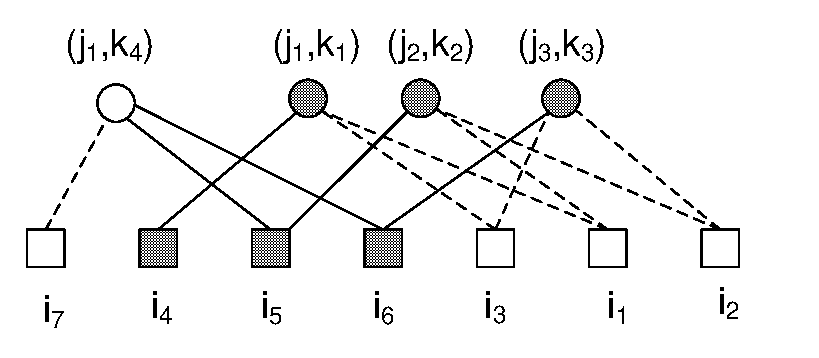
\includegraphics[width=2.7in,height=1.35in]{fig05c.eps}
%\caption{Candidate (3,3) absorbing set (solid circles), with an
%adjacent bit node (empty circle).}\label{Fig05a}
%\end{figure}
\begin{figure}
\center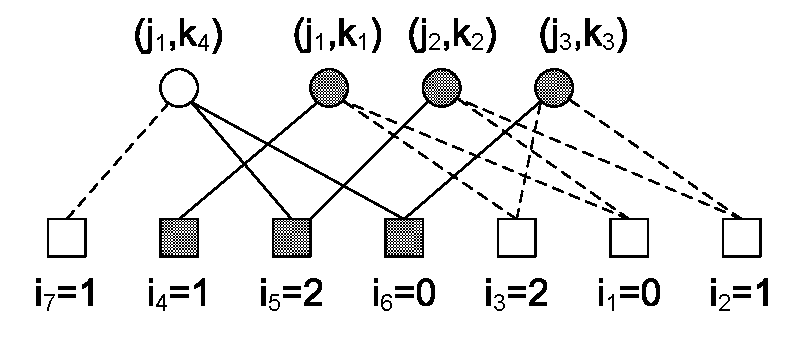
\includegraphics[width=2.9in,height=1.35in]{Visio-fig07z.eps}%{fig05c.eps}
\caption{Candidate (3,3) absorbing set (solid circles), with an
adjacent bit node (empty circle).}\label{Fig05a}
\end{figure}

Suppose first that a $(3,3)$ fully absorbing set exists. Since
$\gamma=3$, it is then necessary that no bit node outside of the
absorbing set participates in more than one unsatisfied check
adjacent to a $(3,3)$ absorbing set. Since $(j_1,k_1)$ and
$(j_3,k_3)$ share a check, $j_1 \neq j_3$. Consider the bit node
labelled $(j_1,k_4)$ that connects to $i_6$, as in Figure
\ref{Fig05a}. Since $i_6=0$, it follows from Corollary
\ref{patterncor} that $k_3=k_4$. Equations
\eqref{eq12a}-\eqref{eq12c} imply that $k_3+2j_1 \equiv k_2+2j_2
\mod p$ so that $(j_1,k_3)$ bit node also connects to the check
labelled $i_5$, as shown in Figure~\ref{Fig05a}. This eliminates the
possibility of a (3,3) fully absorbing set.

A (4,0) absorbing set cannot exist since the minimum distance of the
code is 6 \cite{helles}. The next candidate size for the smallest
fully absorbing set is (4,2). Each of the unsatisfied checks in any
such configuration would necessarily connect to only one of the bit
nodes, else we would have a cycle of length 4, a contradiction
\cite{fan}. Given this, no satisfied check node can connect to all
four bit nodes, else we would have a cycle of length 4, a
contradiction \cite{fan}. Since there are 10 edges from the bit
nodes that go to satisfied checks we now see that there must be 5
satisfied checks in any candidate (4,2) fully absorbing set. The two
bit nodes that each have all their three edges going to satisfied
check nodes must then share exactly one satisfied check (they have
to share at least one, and cannot share more than one \cite{fan}).
We have therefore concluded that any candidate (4,2) fully absorbing
set must look like (an unlabelled version) of Figure~\ref{Fig05a}.
The existence of such (4,2) fully absorbing sets is proved in
Lemma~\ref{le11}, which also counts the number of such
sets.\hfill$\blacksquare$



\comment{Since $i_3=2$ and $i_2=1$, $i_6$ has value 0 ($i_6
\in\{0,1,2\}$ and distinct from $i_2,i_3$ by the bit consistency
condition at $(j_3,k_3)$). Since $j_6=0$, it follows that $k_3=k_4$.
Note that likewise $i_5=2$ in Figure \ref{Fig05a}, since $i_1=0$,
and $i_2=1$, and using the bit consistency condition at the bit node
$(j_3,k_3)$.

If the $(j_1,k_3)$ bit node does not also participate in the check
labelled with $i_5$ it would be necessary that $k_3+2j_1 \neq
k_2+2j_2 \mod p$, which is in contradiction with (\ref{eqpl})
through (\ref{eq12c}). Therefore the bit node $(j_1,k_3)$ shares
checks labelled with $i_5$ and $i_6$ with the bit nodes
$(j_2,k_2)$ and  $(j_3,k_3)$, respectively. This eliminates a
$(3,3)$ fully absorbing set for this configuration. This also now
implies a candidate $(4,2)$ fully absorbing set with bit nodes
$(j_1,k_1), (j_2,k_2)$, $(j_3,k_3)$ and $(j_1,k_3)$. Furthermore,
if a bit node labelled $(j_4,k_4)$ shares checks with the bit
nodes $(j_2,k_2)$ and $(j_,k_3)$ as above, $j_4=j_1$.

The cases where the bit node $(j_1,k_3)$ shares its remaining check,
which we label $i_7$, with one of $(j_1,k_1), (j_2,k_2)$, or
$(j_3,k_3)$ can be eliminated as we now show. By the bit consistency
condition at the bit node $(j_1,k_3)$, $i_7=1$. By the girth
constraint, the bit node $(j_1,k_3)$ cannot share this check with
either $(j_2,k_2)$ or $(j_3,k_3)$. Since the bit node $(j_1,k_1)$
already has the neighboring check whose label is $i_4=1$, if the bit
node $(j_1,k_3)$ also participates in this check, it would imply the
existence of a $(4,0)$ absorbing set, which is impossible since the
minimum distance of this code is 6, \cite{helles}.

Therefore, in the resulting $(4,2)$ absorbing set, the unsatisfied
checks are labelled $i_4$ and $i_7$. Since $i_4=i_7=1$ no bit node
outside of this absorbing set can connect to both unsatisfied
checks, this $(4,2)$ configuration represents a fully absorbing
set.


It can be shown similarly that every $(4,2)$ fully absorbing set
has the shape as the unlabelled configuration in
Figure~\ref{Fig05a}, and that each can be obtained from an
underlying $(3,3)$ absorbing set. In particular, by the girth
condition, each unsatisfied check has degree 1 with respect to the
bits in the absorbing set (and these bits must be different by
definition of an absorbing set) and each neighboring satisfied
check has degree 2 with respect to the bits in the absorbing set.
To ensure that each bit node in the absorbing set has strictly
more satisfied than unsatisfied checks, it is further necessary
that the two bit nodes in the absorbing set with all neighboring
checks satisfied, each share a distinct check with one of the
remaining two bit nodes in the absorbing set, and one satisfied
check with each other. As a result, we arrive at the unlabelled
configuration in Figure~\ref{Fig05a}.


By symmetry, for each underlying $(3,3)$ absorbing set and for
each of the three choices of the labels of the resulting
unsatisfied check, there exists exactly one way of adjoining a
distinct fourth bit node that neighbors these unsatisfied checks.
Since the labels of the two unsatisfied checks are the same, each
resulting $(4,2)$ fully absorbing set comes from two different
$(3,3)$ underlying configurations.

 We complete the section with the following result.} %% end of comment
\begin{lemma}\label{le11} The total number of $(3,3)$ absorbing sets and $(4,2)$ fully absorbing sets
in the Tanner graph described by $H_{p,3}$ is $p^2(p-1)$, and
$3p^2(p-1)/2$, respectively.
\end{lemma}
\comment{\noindent \textit{Proof:} It suffices to consider
$\ell=-1,0,1$ in (\ref{eqpl}) with $i_1=0$, $i_2=1$ and $i_3=2$.

For $\ell=0$, $2j_1=j_2+j_3$. For each value of $j_1$, $1 \leq j_1
\leq (p-1)/2$, there are $2j_1$ ways of assigning values to
$(j_1,j_2,j_3)$ (the cases where two of $j_1$,$j_2$ and $j_3$ are
the same have to be excluded by the check consistency condition).
Likewise, for each $j_1$ where $(p+1)/2 \leq j_1 \leq p-2$ there are
$2(p-1-j_1)$ ways of assigning values to $(j_1,j_2,j_3)$. For each
assignment there are $p$ ways to assign values to $(k_1,k_2,k_3)$ to
ensure the validity of (\ref{eq12a})-(\ref{eq12c}). In all, there is
a total of
\[p\left[\sum_{j_1=1}^{(p-1)/2} 2j_1 + \sum_{j_1=(p+1)/2}^{p-2}
2(p-1-j_1)\right] = \frac{p(p-1)^2}{2}\] such assignments, each
describing a different $(3,3)$ absorbing set.

Likewise, for $\ell=1$ (and for $\ell=-1$ by symmetry) we require
$p+(j_2+j_3)=2j_1$. Thus $s=(j_2+j_3)$ is at most $p-2$ and odd.
For each such $s$, there are $s+1$ ways to assign the values to
$j_1,j_2$ and $j_3$, and for each such assignment, there are $p$
ways to assign values to $(k_1,k_2,k_3)$ to ensure the validity of
(\ref{eq12a})-(\ref{eq12c}). The total number of ways to select a
(3,3) absorbing set in this case is
\[
p\left[\sum_{s=1, s \text{
odd}}^{p-2}(s+1)\right]=\frac{p(p-1)(p+1)}{4}~.
\]

The total number of $(3,3)$ absorbing sets is thus $p^2(p-1)$.

Depending on which two of these three bit nodes the remaining bit
node $(j_4,k_4)$ (in the $(4,2)$ fully absorbing set) shares a
(satisfied) check with, we may assign $(j_4,k_4)$ in three
different ways. Note that in this way we have counted each $(4,2)$
set twice. Hence there are $3p^2(p-1)/2$ distinct $(4,2)$ fully
absorbing sets. \hfill$\blacksquare$

%\begin{corollary} The number of $(3,3)$ absorbing sets in
%$C_{p,3}$ is $O(n^{3/2})$, where $n$ is the codeword length.
%\end{corollary} \noindent \textit{Proof:}

Since the codeword length $n$ is $p^2$, the result of Lemma
\ref{le11} implies Theorem~\ref{theo2} for $\gamma=3$, that is, the
number of minimal absorbing sets as well as the number of minimal
fully absorbing sets grows as $\Theta(n^{3/2})$. Observe that we
have proved  the existence of the minimal fully absorbing sets of
size $(4,2)$. By comparison, the minimum distance of the
$C_{p,\gamma}$ code is $6$, \cite{helles}. } %% end of comment

\noindent \textit{Proof:} Referring to Figure~\ref{Fig05}, the bit
consistency and the check consistency constraints are satisfied for
the given labels of row groups and since $j_1$, $j_2$ and $j_3$ are
distinct. Then $j_1$ and $k_1$ can be chosen in $p$ ways, and then
$j_3$ can be chosen in $p-1$ ways. This fixes $k_3$ by equation
\eqref{eq12a}, $k_2$ by equation \eqref{eq12b} and then $j_2$ by
equation \eqref{eq12c}. There is then a unique way to choose the row
indices in the individual row groups so that the pattern consistency
conditions of Lemma \ref{patternlemma} are satisfied. Thus the total
number of (3,3) absorbing sets is $p^2(p-1)$.

Turning to counting (4,2) fully absorbing set, every such set must
look like an unlabelled version of Figure \ref{Fig05a}, and so
contains exactly two distinct (3,3) absorbing sets (corresponding
respectively to removing one of the bit nodes that connects to an
unsatisfied check). From Figure~\ref{Fig05} one can see that every
(3,3) absorbing set is contained in three distinct (4,2) fully
absorbing sets (for each pair of unsatisfied checks in
Figure~\ref{Fig05} one can find a bit node that these checks connect
to, which when appended to the (3,3) absorbing set gives a (4,2)
fully absorbing set). The total number of (4,2) fully absorbing sets
is therefore $3p^2(p-1)/2$.\hfill$\blacksquare$
\subsection{Absorbing sets of $H_{p,4}$}\label{theo14}
%\subsubsection{Subsubsection Heading Here}
%Subsubsection text here.



In order to establish that $(6,4)$ (fully) absorbing sets are
minimal for $H_{p,4}$, we will first show that $(a,b)$ absorbing
sets for $a < 6$ do not exist.

\comment{First, the condition $a<4$ is not possible as it would
violate the girth condition. For $a=4$, if $b<4$, there would
exist a bit node sharing at least two satisfied checks with some
other bit node in the absorbing set. If $b>4$, there would exist a
bit node in the absorbing set having more unsatisfied that
satisfied checks, which is not possible by definition. Thus, for
$a=4$, the only nontrivial candidate absorbing set is a $(4,4)$
absorbing set. }


Let $D$ denote an $(a,b)$ absorbing set in $G_{p,4}=(V,F,E)$, the
Tanner graph of $H_{p,4}$. If $a=2$ (respectively $3$) then at
least $6$ (respectively $9$) edges from $D$ in $G_{p,4}$ terminate
in $\mathcal{E}(D)$, which implies the existence of a cycle of
length 4 in $G_{p,4}$, which is false \cite{fan}. Thus, $a \geq
4$.

\comment{Suppose $a=4$. The number of edges from $D$ in $G_{p,4}$
that terminate in $\mathcal{E}(D)$ must be 12, 14, or 16,
corresponding to the cases $b$ = 4, 2, or 0, respectively. No check
node in $\mathcal{E}(D)$ can connect to all four of the bit nodes in
$D$, else there would need to be a cycle of length 4 in $G_{p,4}$,
which is false \cite{fan}. Thus, each check node in $\mathcal{E}(D)$
connects to exactly two of the bit nodes in $D$. There are $6$ pairs
of nodes in $D$. Thus we must have $b=4$. The following lemma
establishes that such sets do not exist for large enough prime $p$.}

Suppose $a=4$. Note that $b$ must be even. We cannot have $b=0$,
since this would imply the existence of a codeword of weight $4$,
which is false, \cite{helles}. If $b=2$ one can conclude that there
must be a cycle of length 4 in the code (whether the number of edges
going into unsatisfied checks is 2 or 4), and this is false,
\cite{fan}. Thus we must have $b=4$ and, since each bit node must
have at least three edges going to satisfied checks, the
impossibility of a cycle of length 4 \cite{fan} implies that the
absorbing set can be described as in Figure~\ref{fig44}. In this
figure each vertex represents a distinct bit node of the candidate
(4,4) absorbing set and each edge represents a satisfied check node
that connects to the bit nodes in the absorbing set, that correspond
to its end points in the figure. The following lemma establishes
that such sets do not exist if the prime $p$ is large enough.

\begin{lemma}\label{Lem2} For $p>7$, the Tanner graph family $G_{p,4}$
does not contain any $(4,4)$ absorbing sets.
\end{lemma}
\noindent \textit{Proof:} \comment{No check node satisfied with
respect to the absorbing set has degree $> 2$, as otherwise there
would exist two bit nodes that share two distinct check nodes, which
is not possible by the girth condition \cite{fan}. Similarly, all
bit nodes in an absorbing set have distinct unsatisfied check
nodes.}
%\begin{figure}\hspace{1.0in}
%\begin{picture}(100,150)(0,0)
%\put(10,50){\line(1,0){60}} \put(10,110){\line(1,0){60}}
%\put(10,50){\line(0,1){60}} \put(70,50){\line(0,1){60}}
%\put(10,50){\line(1,1){60}} \put(10,110){\line(1,-1){60}}
%\put(0,40){{$(j_4,k_4)$}} \put(60,120){{$(j_2,k_2)$}}
%\put(0,120){{$(j_1,k_1)$}} \put(60,40){{$(j_3,k_3)$}}
%%\put(255,205){{$c_1^0(11)$='1'}}
%\put(0,80){{$i_4$}} \put(75,80){{$i_2$}} \put(40,120){{$i_1$}}
%\put(40,40){{$i_3$}} \put(31,90){{$i_5$}} \put(31,65){{$i_6$}}
%\end{picture}
%\caption{Depiction of the (4,4) set}
%\end{figure}
\begin{figure}
\center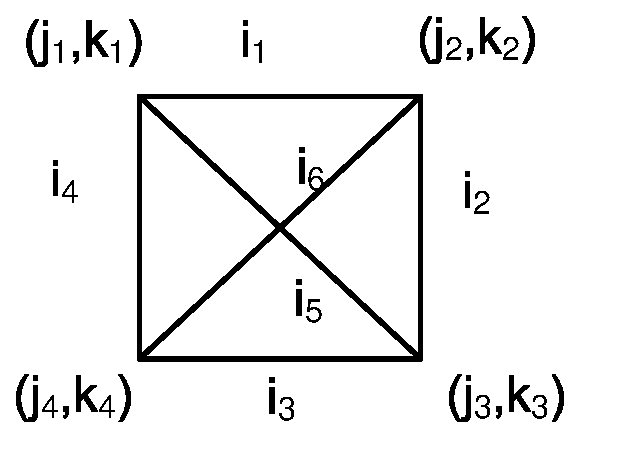
\includegraphics[width=2.65in,height=1.5in]{Drawing10_1.eps}
\caption{Depiction of the candidate (4,4) set} \label{fig44}
\end{figure}
\comment{Since each bit node in the absorbing set shares exactly 3
satisfied check nodes with other bit nodes in the absorbing set, we
can view the absorbing set as shown in Figure \ref{fig44} where each
(labelled) vertex represents a distinct bit node and each (labelled)
edge represents a check node in which the bit nodes associated with
its endpoints participate.} \comment{By the check consistency
condition all $j_1$ through $j_4$ are different. Since the column
$k_1$ of $\sigma^{i_1j_1}$ and column $k_2$ of $\sigma^{i_1j_2}$
have a non-zero entry in the same row, it follows that
\begin{eqnarray*}
k_1+i_1j_1 &\equiv & k_2+i_1j_2 \mod p
\end{eqnarray*}

Likewise, for $i_2$ through $i_6$ we obtain
\begin{eqnarray*}
k_2+i_2j_2 &\equiv& k_3+i_2j_3 \mod p, \\
k_3+i_3j_3 &\equiv& k_4+i_3j_4 \mod p, \\
k_1+i_4j_1 &\equiv& k_4+i_4j_4 \mod p, \\
k_1+i_5j_1 &\equiv& k_3+i_5j_3 \mod p, \text{and}\\
k_2+i_6j_2 &\equiv& k_4+i_6j_4 \mod p.
\end{eqnarray*}}
Without loss of generality we may let $i_1=x$, $i_5=y$ and $i_4=z$,
where $x,y,z \in \{0,1,2,3\}$ and distinct by the bit consistency
conditions. Then, by propagating the bit consistency conditions at
each remaining vertex, and exploiting the symmetry, it suffices to
consider $(i_1,i_2,i_3,i_4,i_5,i_6)$ either $(x,y,x,y,z,z)$ or
$(x,y,x,y,z,w)$ where $x,y,z,w \in \{0,1,2,3 \}$ and are distinct.

For the case $(i_1,i_2,i_3,i_4,i_5,i_6)$ = $(x,y,x,y,z,z)$, we
establish the following cycle consistency conditions based on the
cycles within the graph in Figure \ref{fig44}:
\begin{equation}\label{eq44a}\begin{array}{ccccc}
x(j_2-j_1)+y(j_3-j_2)+z(j_1-j_3) & \equiv 0 \mod p,& \\
x(j_2-j_1)+z(j_4-j_2)+y(j_1-j_4) & \equiv 0 \mod p,&\text{and}\\
x(j_4-j_3)+y(j_1-j_4)+z(j_3-j_1) & \equiv 0 \mod p.&
\end{array}\end{equation}


By adding and subtracting the conditions in~\eqref{eq44a}, it
follows that
\begin{equation}\label{eq44b}\begin{array}{ccccc}
(y-z)(j_3+j_4-j_1-j_2) &\equiv 0 \mod p,&\\
(x-z)(j_2+j_3-j_1-j_4) &\equiv 0 \mod p,&\text{and}\\
(x-y)(j_2+j_4-j_1-j_3) &\equiv 0 \mod p.&
\end{array}\end{equation}

Since $x,y,z$ are distinct, ~\eqref{eq44b} implies that $j$'s would
have to be all the same, which contradicts the check consistency
constraint.

For the case $(i_1,i_2,i_3,i_4,i_5,i_6)$ = $(x,y,x,y,z,w)$, again
based on the cycle structure in Figure \ref{fig44}, we get the cycle
consistency conditions
\begin{equation}\label{eq44c}\begin{array}{ccccc}
x(j_2-j_1)+y(j_3-j_2)+z(j_1-j_3)& \equiv 0 \mod p,&{}\\
x(j_2-j_1)+w(j_4-j_2)+y(j_1-j_4)& \equiv 0 \mod p,&\text{and}\\
x(j_4-j_3)+y(j_1-j_4)+z(j_3-j_1)& \equiv 0 \mod p.&{}
\end{array}\end{equation}


We let $u_1 \asn j_2-j_1$, $u_2 \asn j_3-j_1$, and $u_3 \asn
j_4-j_1$. By the check consistency condition, all of $u_1$, $u_2$,
and $u_3$ are non-zero. Substituting $u_1$, $u_2$ and $u_3$ in
~\eqref{eq44c} and then expressing $u_2$ and $u_3$ in terms of
$u_1$, one arrives at the condition
\begin{equation}\label{eq23}
(z-x)(w-y)+(z-y)(w-x) \equiv 0 \mod p.
\end{equation}

It can be easily verified that this condition can not hold for any
choice of $x,y,z,w$, where $x,y,z,w \in \{0,1,2,3 \}$ and are
distinct for $p>7$. There are $4!=24$ ways of assigning numerical
values to $(x,y,z,w)$. The expression in~\eqref{eq23} is at most $7$
in absolute value for such $x,y,z$, and $w$.  Substituting each
numerical assignment $(x,y,z,w)$ yields possible choices of prime
$p$ for which the expression in~\eqref{eq23} becomes zero $\mod p$.
The condition~\eqref{eq23} holds for $p \in \{2,5,7\}$. Therefore,
for $p>7$, $G_{p,\gamma}$ does not contain $(4,4)$ absorbing
sets.\hfill$\blacksquare$

%(the solutions exist for $p \in \{2,5,7\}$

 We next show that $(5,b)$
absorbing sets do not exist for the parameter $p$ large enough. In
particular we will establish a congruential constraint involving the
labels of the edges emanating from the bits in the absorbing set
that cannot hold for $p$ large enough.
\begin{lemma}\label{Lem3} For $p>19$, the Tanner graph family $G_{p,4}$
does not contain any $(5,b)$ absorbing sets.
 \end{lemma}

\noindent \textit{Proof:} Since each bit node in the absorbing set
has at most one neighboring unsatisfied check node, it follows that
$b \leq 5$. Observe that the number of bit nodes with 3 satisfied
and 1 unsatisfied check nodes is even, and thus $b$ is even. First
$b>0$ by the minimum distance, $d_{min}\geq 8$ of the code,
\cite{helles}. \comment{If $b=2$ and all satisfied check nodes had
degree 2, such an absorbing set would contain a $(4,4)$ absorbing
set, which by Lemma \ref{Lem2} does not exist. A degree-4 satisfied
check node would violate the girth condition. We are thus left with
analyzing $b=4$ with all satisfied check nodes of degree 2. Note
that by the girth condition, all unsatisfied checks have degree 1
with respect to the bits in the absorbing set. Therefore,} If $b=2$,
since we have at most five edges going to unsatisfied checks there
are two cases: (a) either three of them go to one unsatisfied check
and one to another, or (b) one edge goes to each unsatisfied check.
In case (a), because the girth of the Tanner graph is bigger than 4,
\cite{fan}, none of the three bit nodes that share an unsatisfied
check can share a satisfied check. Further, no two bit nodes can
share a satisfied check for the same reason. By counting, this
eliminates case (a). In case (b), if we drop one of the bit nodes
that has an unsatisfied check we would have a (4,4) absorbing set
which we have argued in Lemma~\ref{Lem2} does not exist for $p>7$.

Thus for $p>7$ we are left with considering the case $b=4$ since at
most five edges go into unsatisfied checks. This means the
 candidate absorbing set contains 1 bit node with all checks
satisfied and 4 bit nodes each with 3 satisfied and 1 unsatisfied
check. The only way that such an absorbing set could exist is if one
has the configuration shown in Figure \ref{fig52}, where the
vertices represent bit nodes and edges represent their satisfied
check nodes.
%we have that $i_1$ connect $(k_1,j_1)$ and
%$(k_2,j_2)$, $i_2$ connect $(k_1,j_1)$ and $(k_3,j_3)$, $i_3$
%connect $(k_1,j_1)$ and $(k_4,j_4)$, $i_4$ connect $(k_1,j_1)$ and
%$(k_5,j_5)$, $i_5$ connect $(k_2,j_2)$ and $(k_3,j_3)$, $i_6$
%connect $(k_2,j_2)$ and $(k_4,j_4)$, $i_7$ connect $(k_3,j_3)$ and
%$(k_5,j_5)$, and $i_8$ connect $(k_4,j_4)$ and $(k_5,j_5)$, as

%\begin{figure}\hspace{1.0in}
%\begin{picture}(100,150)(0,0)
%\put(10,50){\line(1,0){60}} \put(10,110){\line(1,0){60}}
%\put(10,50){\line(0,1){60}} \put(70,50){\line(0,1){60}}
%\put(10,50){\line(1,1){60}} \put(10,110){\line(1,-1){60}}
%\put(0,40){{$(j_4,k_4)$}} \put(60,120){{$(j_2,k_2)$}}
%\put(0,120){{$(j_1,k_1)$}} \put(60,40){{$(j_3,k_3)$}}
%%\put(255,205){{$c_1^0(11)$='1'}}
%\put(0,80){{$i_4$}} \put(75,80){{$i_2$}} \put(40,120){{$i_1$}}
%\put(40,40){{$i_3$}} \put(31,90){{$i_5$}} \put(31,65){{$i_6$}}
%\end{picture}
%\caption{Depiction of the candidate (5,2) set}
%\end{figure}

\begin{figure}
\center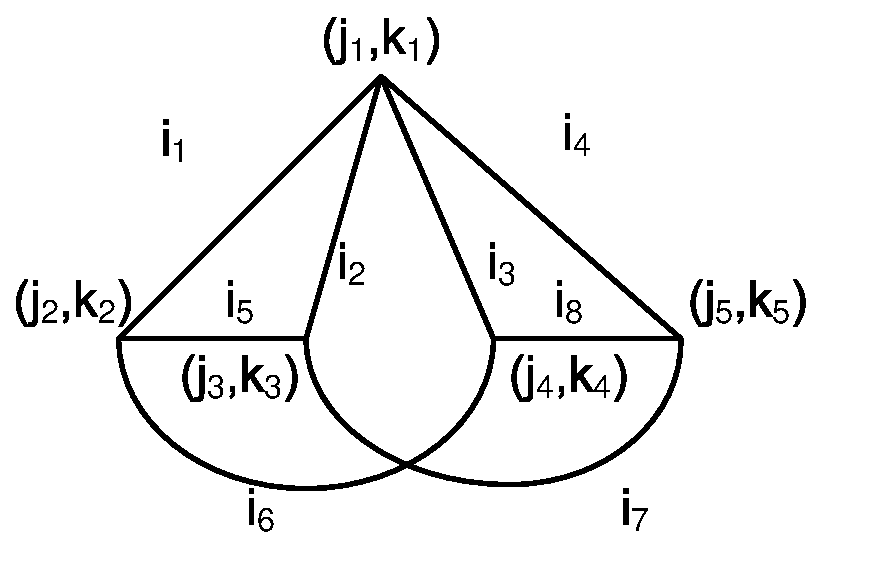
\includegraphics[width=3.0in,height=1.8in]{Drawing22_1.eps}
\caption{Depiction of the candidate (5,4) set} \label{fig52}
\end{figure}

Since $i_1$, $i_2$, $i_3$ and $i_4$ are all distinct elements of the
set $\{0,1,2,3\}$, by the bit consistency condition, and by the
symmetry of the candidate configuration in Figure~\ref{fig52}, we
may assume that $i_1=0$. We let $x \asn i_2$, $y \asn i_3$ and $z
\asn i_4$, where $x,y,z \in \{1,2,3 \}$ and distinct. By propagating
possible values of the labels for remaining edges, while maintaining
bit consistency conditions, it follows that
$(i_1,i_2,i_3,i_4,i_5,i_6,i_7,i_8)$ is either $(0,x,y,z,y,z,0,x)$ or
$(0,x,y,z,z,x,y,0)$.

For $(i_1,i_2,i_3,i_4,i_5,i_6,i_7,i_8)$ = $(0,x,y,z,y,z,0,x)$, and
for each edge and its endpoints in Figure~\ref{fig52}, we write the
pattern consistency constraints of Corollary~\ref{patterncor}, in
terms of $x$, $y$ and $z$,
\begin{subequations}\label{eq52a}\begin{eqnarray}
\label{eq52a1}k_1 &\equiv& k_2 \mod p,\\
\label{eq52a2}k_3 &\equiv& k_5 \mod p,\\
\label{eq52a3}k_1+xj_1 &\equiv& k_3+xj_3 \mod p, \\
\label{eq52a4}k_1+yj_1 &\equiv& k_4+yj_4 \mod p, \\
\label{eq52a5}k_1+zj_1 &\equiv& k_5+zj_5 \mod p, \\
\label{eq52a6}k_2+yj_2 &\equiv& k_3+yj_3 \mod p, \\
\label{eq52a7}k_2+zj_2 &\equiv& k_4+zj_4 \mod p, \text{and}\\
\label{eq52a8}k_4+xj_4 &\equiv& k_5+xj_5 \mod p.
\end{eqnarray}\end{subequations}

This last system simplifies to
\begin{equation}\label{eq52b}\begin{array}{llllll}
k_1+xj_1 &\equiv& k_3+xj_3 \mod p,& {}&\text{(from \eqref{eq52a3})}\\
k_1+yj_1 &\equiv& k_4+yj_4 \mod p,& {}&\text{(from \eqref{eq52a4})}\\
k_1+zj_1 &\equiv& k_3+zj_5 \mod p,& {}&\text{(from \eqref{eq52a2} and \eqref{eq52a5})}\\
k_1+yj_2 &\equiv& k_3+yj_3 \mod p,& {}&\text{(from \eqref{eq52a1} and \eqref{eq52a6})}\\
k_1+zj_2 &\equiv& k_4+zj_4 \mod p, &\text{and}&\text{(from \eqref{eq52a1} and \eqref{eq52a7})}\\
k_4+xj_4 &\equiv& k_3+xj_5 \mod p.&{}&\text{(from \eqref{eq52a2} and
\eqref{eq52a8})}
\end{array}\end{equation}

Thus
\begin{subequations}\begin{eqnarray}
\label{eq52s1}k_1-k_3 &\equiv x(j_3-j_1) \equiv z(j_5-j_1) \equiv
y(j_3-j_2) &
\mod p\\
\label{eq52s2}k_1-k_4 &\equiv y(j_4-j_1) \equiv z(j_4-j_2) &
\mod p\\
\label{eq52s3}k_3-k_4 &\equiv x(j_4-j_5) &\mod p.
\end{eqnarray}\end{subequations}

 We let $u_1 \asn j_3 -j_1$, $u_2\asn j_4 -j_1$, $u_3 \asn j_4
-j_1$, and $u_4 \asn j_3 -j_2$. Note that by the check consistency
condition, all of $u_1$, $u_2$, $u_3$, and $u_4$ are non-zero.

We then obtain
\begin{equation}\begin{array}{cccccc}
xu_1 &\equiv& zu_3 & \mod p & \text{(from \eqref{eq52s1}),} \\xu_1
&\equiv& yu_4 & \mod p & \text{(from \eqref{eq52s1}),}\\
yu_2 &\equiv& z(u_2-u_1+u_4)& \mod p & \text{(from \eqref{eq52s2}),}
\\x(u_2-u_3)
&\equiv& yu_2-xu_1 & \mod p & \text{from
$k_3-k_4=(k_1-k_4)-(k_1-k_3)$ and }\\{}&{}&{}&{}& \text{substituting
from \eqref{eq52s3},\eqref{eq52s2},\eqref{eq52s1}),resp.}
\end{array}\end{equation}

This last system can be rewritten as
\begin{equation}\label{sys52a}
\left[ \begin{array}{ccccccc} x & 0 & 0 & -y\\
x & 0 & -z &0\\
-z & z-y &0 & z\\
-x & y-x & x & 0
\end{array}\right] \left[\begin{array}{c}
u_1\\u_2\\u_3\\u_4 \end{array}\right] \equiv
\left[\begin{array}{c}0\\0\\0\\0\end{array}\right] \mod p~.
\end{equation}

Therefore, the determinant of the matrix multiplying the (non-zero)
vector $\left[u_1 u_2 u_3 u_4\right]^{T}$ in ~\eqref{sys52a} is
itself zero, which simplifies to
\begin{equation}\label{eq5a}
xy(z-x)(z-y)-z^2(x-y)^2 \equiv 0 \mod p,
\end{equation}

Since $x,y,z \in \{1,2,3\}$ and distinct we consider all $3!=6$
assignment for $(x,y,z)$, and for each we evaluate the left had side
expression in~\eqref{eq5a}. Note that for distinct $x,y,z \in
\{1,2,3\}$ , this expression is at most $19$ in absolute value, and
therefore the constraint in ~\eqref{eq5a} does not have a solution
for $p>19$ for distinct $x,y,z \in \{1,2,3\}$. (Solutions exist for
$p=5,11$ and $19$, which can be verified by direct numerical
substitution).

For $(i_1,i_2,i_3,i_4,i_5,i_6,i_7,i_8)$ = $(0,x,y,z,z,z,y,0)$ we
likewise establish the constraints as in \eqref{eq52a} and
\eqref{eq52b}. We again let $u_1 \asn j_3 -j_1$, $u_2\asn j_4
-j_1$, $u_3 \asn j_4 -j_1$, and $u_4 \asn j_3 -j_2$, and obtain
\begin{equation}\label{sys52b}
\left[ \begin{array}{ccccccc} 0 & y & -z & 0\\
x & y-x & 0 & -x\\
x & 0 &0 & -z\\
y-x & y & -y & 0
\end{array}\right] \left[\begin{array}{c}
u_1\\u_2\\u_3\\u_4 \end{array}\right] \equiv
\left[\begin{array}{c}0\\0\\0\\0\end{array}\right] \mod p~.
\end{equation}

Since the entries in  $\left[u_1 u_2 u_3 u_4\right]^{T}$ are all
non-zero, it follows that the determinant of the matrix
in~\eqref{sys52b} is zero. Simplifying the expression for the
determinant yields again the condition in \eqref{eq5a}. Therefore
for $p>19$, (5,4) absorbing sets do not exist.\hfill$\blacksquare$

\comment{ and likewise for $i_8=0$ we let $x=i_2=i_6$, $y=i_3=i_7$
and $z=i_4=i_5$. Note that now $k_1=k_2$ and $k_4=k_5$ and
\begin{eqnarray*}
k_1+xj_1 &\equiv& k_3+xj_3 \mod p, \\
k_1+yj_1 &\equiv& k_4+yj_4 \mod p, \\
k_1+zj_1 &\equiv& k_5+zj_5 \mod p, \\
k_2+zj_2 &\equiv& k_3+zj_3 \mod p, \\
k_2+xj_2 &\equiv& k_4+xj_4 \mod p, \text{and}\\
k_3+yj_3 &\equiv& k_5+yj_5 \mod p.
\end{eqnarray*}

where $x,y,z\in \{1,2,3\}$ and distinct.}

\comment{In both cases, after some algebra we arrive at
\begin{equation}\label{eq5a}
xy(z-x)(z-y)-z^2(x-y)^2 \equiv 0 \mod p,
\end{equation}
which does not have a solution for $p>19$ for distinct $x,y,z \in
\{1,2,3\}$.\hfill$\blacksquare$ %\footnote{As a side remark, we note that equation
%(\ref{eq5a}) does have a solution for $p \in \{5,11,19$\}.}
}
%No 4 deg. checks. dmin is 8.
%\begin{remark}

We can now proceed with the analysis of $(6,b)$ absorbing sets.
Since the number of bit nodes with 3 satisfied and 1 unsatisfied
check node is even, $b$ is even. First, $b=0$ is not possible
since $d_{min} \geq 8$ \cite{helles}. The following lemma
considers $b=2$.

\comment{ Observe that there cannot be a check of degree 4 with
respect to the bits in a $(6,b)$ absorbing set, as otherwise the
girth condition would be violated. As a result, in the remainder
of the analysis we will assume that all checks that have even
number of bit node neighbors in a $(6,b)$ absorbing set have
degree 2 with respect to the absorbing set. Moreover, since
$d_{min} \geq 8$ \cite{helles} and since all bit nodes in the
$(6,b)$ absorbing set have at most one unsatisfied check (with
respect to the absorbing set), it suffices to consider $b$ even
and positive.}
%\end{remark}

\begin{lemma}\label{Lem4} For $p>19$, the Tanner graph family $G_{p,4}$ does not contain any $(6,2)$ absorbing sets.
\end{lemma}

\noindent \textit{Proof:}
%\begin{figure}\hspace{1.0in}
%\begin{picture}(100,150)(0,0)
%\put(10,50){\line(1,0){60}} \put(10,110){\line(1,0){60}}
%\put(10,50){\line(0,1){60}} \put(70,50){\line(0,1){60}}
%\put(10,50){\line(1,1){60}} \put(10,110){\line(1,-1){60}}
%\put(0,40){{$(j_4,k_4)$}} \put(60,120){{$(j_2,k_2)$}}
%\put(0,120){{$(j_1,k_1)$}} \put(60,40){{$(j_3,k_3)$}}
%%\put(255,205){{$c_1^0(11)$='1'}}
%\put(0,80){{$i_4$}} \put(75,80){{$i_2$}} \put(40,120){{$i_1$}}
%\put(40,40){{$i_3$}} \put(31,90){{$i_5$}} \put(31,65){{$i_6$}}
%\end{picture}
%\begin{picture}(100,150)(0,0)
%\put(10,50){\line(1,0){60}} \put(10,110){\line(1,0){60}}
%\put(10,50){\line(0,1){60}} \put(70,50){\line(0,1){60}}
%\put(10,50){\line(1,1){60}} \put(10,110){\line(1,-1){60}}
%\put(0,40){{$(j_4,k_4)$}} \put(60,120){{$(j_2,k_2)$}}
%\put(0,120){{$(j_1,k_1)$}} \put(60,40){{$(j_3,k_3)$}}
%%\put(255,205){{$c_1^0(11)$='1'}}
%\put(0,80){{$i_4$}} \put(75,80){{$i_2$}} \put(40,120){{$i_1$}}
%\put(40,40){{$i_3$}} \put(31,90){{$i_5$}} \put(31,65){{$i_6$}}
%\end{picture}
%\caption{Depiction of the candidate (6,2) sets}
%\end{figure}
\begin{figure}
\center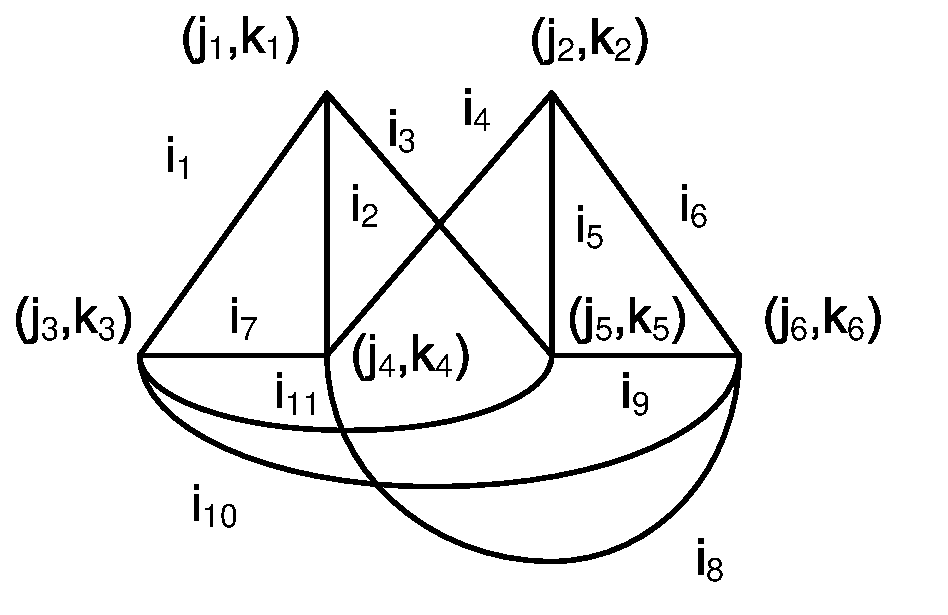
\includegraphics[width=2.8in,height=1.8in]{Drawing30_2.eps}
\center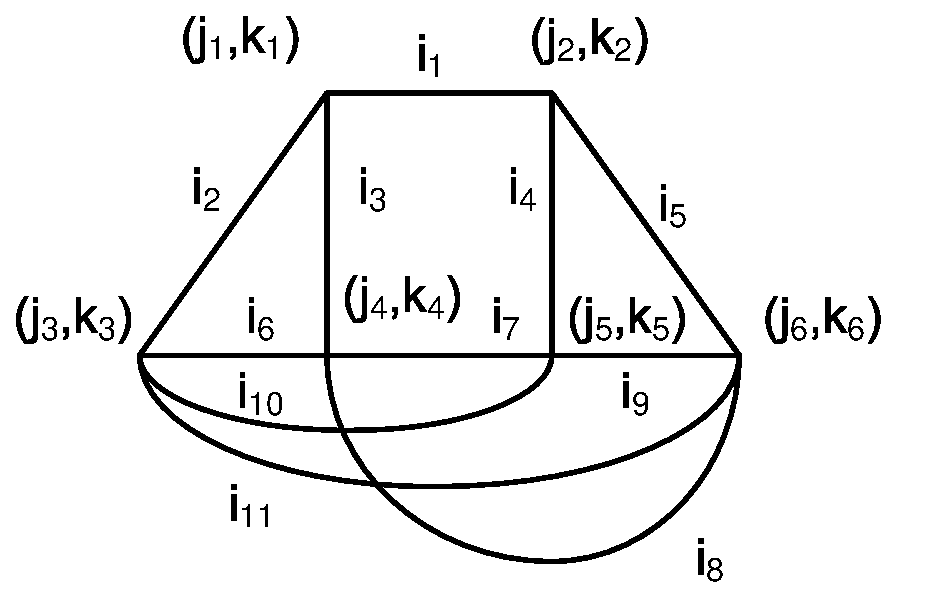
\includegraphics[width=2.8in,height=1.8in]{Drawing32_1.eps}\hspace{0.3in}
\caption{Depiction of the candidate (6,2) sets.} \label{fig62}
\end{figure}
\comment{We first claim that there is no check node of degree at
least 4 with respect to the bit nodes in the absorbing set. Indeed,
if this were to occur, there would exist at least 2 bit nodes in the
absorbing set with all check nodes satisfied and with a shared check
node of degree at least 4. They would necessarily share another
check node, which is not possible by the girth condition \cite{fan}.

We can now focus on the case where all satisfied check nodes with
respect to the absorbing set have degree 2. By requiring that each
vertex corresponding to a bit node in the absorbing set has either 3
or 4 outgoing edges, and that there are no parallel edges, it
follows that there are 2 possible configurations, as shown in Figure
\ref{fig62}, that relate bit nodes in the absorbing set (vertices)
and their shared satisfied checks (edges). Note that it is apriori
possible to have an unsatisfied check of degree 3 with respect to
the bit nodes in the absorbing set. This condition is not a part of
Figure\ref{fig62}.} %%% end comment
We first claim that there is no check node of degree at least 3 with
respect to the bit nodes in the absorbing set. Let us first suppose
that there exists one such check node and that it has an even degree
with respect to the bit nodes in the absorbing set. Since we are
considering an absorbing set with 6 bit nodes, such a check node
would have degree either 4 or 6 with respect to the bit nodes in the
absorbing set. If this satisfied check is of degree 6, there would
exist 2 bit nodes in the absorbing set which would share an
additional satisfied check. This situation would imply the existence
of a cycle of length 4, which is impossible by the girth condition
\cite{fan}.

Suppose now that this satisfied check has degree 4. Each bit node
that participates in this check has at least 2 more neighboring
satisfied checks, which it then necessarily must share with the
remaining two bit nodes in the absorbing set that themselves do not
participate in this degree-4 check. If there exists a bit node that
participates in this degree-4 check and has all checks satisfied, it
then shares its remaining neighboring check with one of the bit
nodes with which it already shares a check. This situation violates
the girth constraint \cite{fan}. If all bit nodes in the absorbing
set that participate in this degree-4 check have 3 satisfied and 1
unsatisfied check, three of them would have to participate in the
same unsatisfied check to make the total number of unsatisfied
checks be 2. This again violates the girth condition \cite{fan}.

Therefore, all satisfied checks with respect to the bit nodes in the
absorbing set have degree 2. Suppose there exists a check node that
is unsatisfied with respect to the bits in the absorbing set and
that has degree bigger than 1. If such a check node has degree 5,
there would necessarily exist 2 bit nodes in the absorbing set that
share this degree-5 check and another satisfied check, which is
impossible by the girth condition.

Suppose that there exists 2 degree-3 checks incident to the bit
nodes in the absorbing set. First, these degree-3 checks do not have
any neighboring bit nodes in common since we require that each bit
node has at most 1 unsatisfied check. We can then group the bit
nodes in the absorbing set into two disjoint groups, each of size 3,
such that the bits in the same group share the same degree-3 check.
Consider a bit node in, say, the first group. It shares its
remaining 3 (satisfied) checks with one of each bit nodes in the
second group. The same is true with the other two bit nodes in the
first group, namely they too share their remaining 3 (satisfied)
checks with the bit nodes in the second group. Therefore, there
exist two bit nodes in the first group and two bit nodes in the
second group such that any two share a distinct check. This
configuration is not possible by Lemma~\ref{Lem2} for $p>7$.

Suppose now there exists one unsatisfied check of degree 3 with
respect to the bit nodes in the absorbing set. The remaining
unsatisfied check then has degree 1 with respect to the bit nodes in
the absorbing set, and the neighboring bit nodes in the absorbing
set of these two unsatisfied checks are different. There are two bit
nodes in the absorbing set that have all checks satisfied. Partition
the bit nodes in the absorbing set into three groups: the first
group contains the three  bit nodes that share a degree-3
unsatisfied check, the second group contains the one bit node that
has one unsatisfied check, and the third group contains the two bit
nodes that have all four checks satisfied. Each of the three bit
nodes in the first group has one unsatisfied and three satisfied
checks and thus it shares a satisfied check with each of the bit
nodes in the second and third group since it cannot share a
satisfied check with another bit node in the first group by the
girth condition. The bit node in the second group also has one
unsatisfied and three satisfied checks, and the latter are shared
then with bit nodes in the first group. The two bit nodes in the
third group have all four checks satisfied, the three of which they
each share with each of the bit nodes in the first group. Since all
three satisfied checks of the bit node in the second group are used
up with the checks it shares with the bit nodes in the first group,
the two bit nodes in the third group share a satisfied check with
each other. Therefore, there exist two bit nodes in the first group
and two bit nodes in the third group such that any two share a
distinct check. This configuration is not possible by
Lemma~\ref{Lem2} for $p>7$.

We conclude that no check incident to the bit nodes in the absorbing
set has degree larger than 2, namely that all neighboring satisfied
(resp. unsatisfied) checks have degree 2 (resp. 1). By requiring
that each vertex corresponding to a bit node in the absorbing set
has either 3 or 4 outgoing edges, and that there are no parallel
edges, it follows that there are 2 possible configurations, as shown
in Figure~\ref{fig62}, that relate bit nodes in the absorbing set
(vertices) and their shared satisfied checks (edges).

Observe that the bottom configuration in Figure~\ref{fig62}
contains a $(4,4)$ absorbing set which consists of $(j_3,k_3)$,
$(j_4,k_4)$, $(j_5,k_5)$, and $(j_6,k_6)$. By Lemma \ref{Lem2}
such configuration is not possible for $p>7$. The rest of the
proof focuses on the topmost configuration.

%%%%%%%%%%%%%%%%%%%%%%%%%%%%%%%%%%%%%%%%%%%%%%%%%%%%%%%%%%%
 By ensuring the bit consistency, it follows that the topmost
configuration in Figure~\ref{fig62} has 2 distinct edge labellings.
In particular, by the bit consistency at $(j_3,k_3)$ we may let $x
\asn i_1$, $y \asn i_7$, $z \asn i_{11}$ and $w \asn i_{10}$, where
$x,y,z,w \in \{0,1,2,3\}$ and distinct. By propagating the labels
while making sure that the bit consistency constraints are satisfied
we obtain

\comment{Specifically, using the bit consistency condition, we have
for the top configuration
\begin{subequations}\begin{eqnarray}
k_1+i_1j_1 &\equiv& k_3+i_1j_3 \mod p, \\
k_1+i_2j_1 &\equiv& k_4+i_2j_4 \mod p, \\
k_1+i_3j_1 &\equiv& k_5+i_3j_5 \mod p, \\
k_2+i_4j_2 &\equiv& k_4+i_4j_4 \mod p, \\
k_2+i_5j_2 &\equiv& k_5+i_5j_5 \mod p, \\
k_2+i_6j_2 &\equiv& k_6+i_6j_6 \mod p, \\
k_3+i_7j_3 &\equiv& k_4+i_7j_4 \mod p, \\
k_4+i_8j_4 &\equiv& k_6+i_8j_6 \mod p, \\
k_5+i_9j_5 &\equiv& k_6+i_9j_6 \mod p, \\
k_3+i_{10}j_3 &\equiv& k_6+i_{10}j_6 \mod p,\text{and} \\
k_3+i_{11}j_3 &\equiv& k_5+i_{11}j_5 \mod p,
\end{eqnarray*}}

\begin{itemize}
\item $x=i_1=i_5=i_8$, $y=i_7=i_9$, $z=i_2=i_6=i_{11}$,
$w=i_3=i_4=i_{10}$ (call this set of constraints $\star$) or \item
$x=i_1=i_4=i_9$, $y=i_3=i_6=i_7$, $z=i_8=i_{11}$,
$w=i_2=i_5=i_{10}$ (call this set of constraints $\star\star$)
where throughout $x,y,z,w$ are distinct and belong to the set
$\{0,1,2,3\}$.
\end{itemize}

\comment{We will now show that in each case we arrive at one of the
following constraints:
\begin{equation}\label{consti}
\begin{array}{ccccc}
\tilde{x} &\equiv& \tilde{y} &\mod p, &\text{or} \\
\tilde{x}\tilde{z}(\tilde{z}-\tilde{y})(\tilde{x}-\tilde{y})
&\equiv& \pm \tilde{y}^2(\tilde{x}-\tilde{z})^2  &\mod p, &{}
\end{array}
\end{equation}

where $\{\tilde{x},\tilde{y},\tilde{z}\} = \{x,y,z\}= \{1,2,3\}$ and
are distinct.

Note that exactly one of $x,y,z,w$ has value $0$, and the remainder
three constitute the set $\{1,2,3\}$.}

\underline{Case ($\star$)}

Using the pattern consistency constraint (see
Corollary~\ref{patterncor}) for each edge in Figure~\ref{fig62} for
the current labelling we obtain
\begin{subequations}\begin{eqnarray}
\label{ar62a}k_1+xj_1 &\equiv& k_3+xj_3 \mod p, \\
\label{ar62b}k_1+zj_1 &\equiv& k_4+zj_4 \mod p, \\
\label{ar62c}k_1+wj_1 &\equiv& k_5+wj_5 \mod p, \\
\label{ar62d}k_2+wj_2 &\equiv& k_4+wj_4 \mod p, \\
\label{ar62e}k_2+xj_2 &\equiv& k_5+xj_5 \mod p, \\
\label{ar62f}k_2+zj_2 &\equiv& k_6+zj_6 \mod p, \\
\label{ar62g}k_3+yj_3 &\equiv& k_4+yj_4 \mod p, \\
\label{ar62h}k_4+xj_4 &\equiv& k_6+xj_6 \mod p, \\
\label{ar62i}k_5+yj_5 &\equiv& k_6+yj_6 \mod p, \\
\label{ar62j}k_3+wj_3 &\equiv& k_6+wj_6 \mod p,\text{and} \\
\label{ar62k}k_3+zj_3 &\equiv& k_5+zj_5 \mod p,
\end{eqnarray}\end{subequations}



We now separately consider $x=0$, $y=0$, $z=0$, and $w=0$.

\noindent 1. For $x=0$, the set of
constraints~\eqref{ar62a}-\eqref{ar62k} reduces to
\begin{equation}\begin{array}{llllllllllll}
k_1-k_3 \equiv 0 \mod p \hspace{1in}\text{(from \eqref{ar62a})}
\\
k_2-k_5 \equiv 0 \mod p \hspace{1in}\text{(from \eqref{ar62e})}
\\
k_4-k_6 \equiv 0 \mod p  \hspace{1in}\text{(from \eqref{ar62h})}
\\ k_1-k_4 \equiv
z(j_4-j_1) \equiv y(j_4-j_3) \equiv w(j_6-j_3) \mod p \\
\hspace{1in}\text{(from \eqref{ar62b}),}\text{ \eqref{ar62a} and
\eqref{ar62g}},\text{ and} \text{ \eqref{ar62a} and
\eqref{ar62j}}\text{ respectively.)}
\\
k_2-k_4 \equiv w(j_4-j_2) \equiv  z(j_6-j_2) \equiv y(j_6-j_5) \mod
p \\ \hspace{1in}\text{(from \eqref{ar62d})}\text{ \eqref{ar62h} and
\eqref{ar62f}},\text{ and{}{} \eqref{ar62e}},\text{\eqref{ar62h} and
\eqref{ar62i}}\text{ respectively.)}
\\
k_1-k_2 \equiv w(j_5-j_1) \equiv z(j_5-j_3) \mod p~.\\
\hspace{1in}(\text{from \eqref{ar62c}}\text{ \eqref{ar62d} and
\eqref{ar62k}} \text{ respectively.})
\end{array}\end{equation}

\noindent Since $j_1 \neq j_4$, $j_2 \neq j_4$ and $j_1 \neq j_5$ by
the check consistency conditions, we have that $k_1 \neq k_4$, $k_2
\neq k_4$ and $k_1 \neq k_2$.

\noindent Since $\{y,z,w\}=\{1,2,3\}$ and $p>19$ is prime, we may
let
\begin{equation}\begin{array}{ccccc}k_1-k_4 &\equiv& ywzt &\mod p, &{} \\
k_2-k_4 &\equiv& ywzu &\mod p, &\text{ and }\\k_1-k_2 &\equiv& wzs
&\mod p&{}
\end{array}\end{equation}
for some integers $t,s$ and $u$ which are themselves nonzero. From
$k_1-k_2=(k_1-k_4)-(k_2-k_4)$, it follows that
\begin{equation}\label{eq621}
wzs \equiv yzwt -ywzu \mod p~.
\end{equation}
Write $j_5-j_3=-(j_6-j_5)+(j_6-j_3)$ to obtain
\begin{equation}\label{eq622}
ws \equiv -wzu +yzt \mod p~.
\end{equation}
Likewise, from $j_5-j_1=-(j_6-j_5)+(j_6-j_2)-(j_4-j_2)+(j_4-j_1)$,
it follows that
\begin{equation}\label{eq623}
zs \equiv -wzu +ywu -yzu +ywt \mod p~.
\end{equation}
\comment{\begin{equation}\begin{array}{cccc}
s &\equiv &yt-yu &\mod p \\
ws &\equiv &-wzu +yzt &\mod p\\
zs &\equiv &-wzu +ywu -yzu +ywt &\mod p~.
\end{array}\end{equation}}
From~\eqref{eq621}-~\eqref{eq623}, by equating the expressions for
$ws$ and $zs$, it follows that
\begin{equation}\begin{array}{cccc}
wu(y-z) &\equiv &yt(w-z) &\mod p \\
wu(y-z) &\equiv &yt(z-w) &\mod p~.
\end{array}\end{equation}
The last set of constraints implies $w\equiv z \mod p$ which is a
contradiction. % with the bit consistency constraint for the bit
%node $(j_3,k_3)$. Note that this is precisely the first condition in
%\eqref{consti} with the substitution $w=\tilde{x}$ and
%$z=\tilde{y}$.
2. For $y=0$ the set of constraints~\eqref{ar62a}-\eqref{ar62k}
reduces to
\begin{equation}\begin{array}{cccccccccc}
k_3-k_4 &\equiv& 0 & {}& {}&{}&{}&\mod p
\\
k_5-k_6 &\equiv& 0 & {}& {}&{}&{}&\mod p\\
k_1-k_3 &\equiv& x(j_3-j_1)& \equiv& z(j_4-j_1)& {} &{}&\mod p
\\
k_2-k_5 &\equiv& x(j_5-j_2) &\equiv&  z(j_6-j_2) &{}&{} &\mod
p\\
k_3-k_5 &\equiv& x(j_6-j_4) &\equiv& w(j_6-j_3) &
\equiv& z(j_5-j_3)&\mod p\\
k_1-k_5 &\equiv& w(j_5-j_1) & {} & {} &{}&{}&\mod p~.
\end{array}\end{equation}
Note that $j_1 \neq j_3$, $j_2 \neq j_5$, $j_4 \neq j_6$ and $j_1
\neq j_5$ by the check consistency conditions. Since
$\{x,z,w\}=\{1,2,3\}$, we may let
\begin{equation}\begin{array}{ccccc}k_1-k_3 &\equiv& xzs &\mod p, &{} \\
k_1-k_5 &\equiv & wv &\mod p, &{}\\ k_2-k_5 &\equiv& xzu &\mod p,
&\text{ and }\\k_3-k_5 &\equiv& xwzt &\mod p&{}
\end{array}\end{equation}
for some integers $s,u,v$ and $t$, which are themselves nonzero. The
identities $k_1-k_3=(k_1-k_5)-(k_3-k_5)$,
$j_5-j_1=(j_5-j_3)+(j_3-j_1)$ and
$j_4-j_1=-(j_6-j_4)+(j_6-j_3)+(j_3-j_1)$ respectively, yield the
following constraints,
\begin{equation}\begin{array}{cccc}
xzs &\equiv &wv-xwzt &\mod p \\
v &\equiv &xwt+zs &\mod p \\
xs & \equiv& -wzt +xzt+zs &\mod p~.
\end{array}\end{equation}
Eliminating $v$ from the top two constraints implies $zs(x-w)
\equiv xwt(w-z) \mod p$, which combined with the bottom constraint
yields
\begin{equation}
z^2(x-w)^2 \equiv xw(w-z)(x-z) \mod p~.
\end{equation}
Since $\{x,y,w\}=\{1,2,3\}$, this cannot hold for $p>19$.

\noindent 3. For $z=0$ we obtain
\begin{equation}\begin{array}{ccccccccc}
k_1-k_4 &\equiv& 0 & {}& {}&{}&{}&\mod p
\\
k_2-k_6 &\equiv& 0 & {}& {}&{}&{}&\mod p\\
k_3-k_5 &\equiv& 0 & {}& {}&{}&{}&\mod p\\
k_1-k_3 &\equiv& x(j_3-j_1)& \equiv& w(j_5-j_1)& \equiv&
y(j_3-j_4) &\mod p
\\
k_2-k_3 &\equiv& x(j_5-j_2) &\equiv&  y(j_5-j_6) &\equiv&
w(j_3-j_6) &\mod
p\\
k_1-k_2 &\equiv& w(j_2-j_4) &\equiv& x(j_6-j_4) & {}&{}&\mod p~.
\end{array}\end{equation}
As before, some algebra yields $x\equiv w \mod p$, a contradiction.
%which with the substitution $x=\tilde{x}$, $y=\tilde{y}$ corresponds
%to the first condition in \eqref{consti}.

\noindent 4. For $w=0$ we obtain
\begin{equation}\begin{array}{ccccccccc}
k_1-k_5 &\equiv& 0 & {}& {}&{}&{}&\mod p
\\
k_2-k_4 &\equiv& 0 & {}& {}&{}&{}&\mod p\\
k_3-k_6 &\equiv& 0 & {}& {}&{}&{}&\mod p\\
k_1-k_3 &\equiv& x(j_3-j_1)& \equiv& y(j_6-j_5)& \equiv&
z(j_3-j_5) &\mod p
\\
k_2-k_3 &\equiv& z(j_6-j_2) &\equiv&  y(j_3-j_4) &\equiv&
x(j_6-j_4) &\mod
p\\
k_1-k_2 &\equiv& z(j_4-j_1) &\equiv& x(j_2-j_5) & {}&{}&\mod p~.
\end{array}\end{equation}

After some algebra, we obtain the following condition
\begin{equation}
xz(z-y)(x-y) \equiv -y^2(x-z)^2 \mod p,
\end{equation}
which, because $\{x,y,z\}=\{1,2,3\}$ has no solution for $p>19$.% can
%be seen to correspond to the second condition in \eqref{consti} with
%the minus sign on the right hand side and the substitution
%$x=\tilde{x}$, $y=\tilde{y}$, and $z=\tilde{z}$.

\underline{Case ($\star\star$)}

We separately consider $x=0$, $y=0$, $z=0$, and $w=0$, and proceed
along the lines of the previous case.% to arrive at the desired
%conditions \eqref{consti}.

For $x=0$, resp. $y=0$, it follows after some algebra that $y \equiv
w \mod p$, resp. $x \equiv w \mod p$, a contradiction in each case.
%which is precisely the first condition in \eqref{consti} with the
%substitution $y=\tilde{x}$ and $w=\tilde{y}$, resp. $x=\tilde{x}$
%and $w=\tilde{y}$.


For $z=0$, resp. $w=0$, it follows similarly that $xw(w-y)(x-y)
\equiv y^2(x-w)^2 \mod p$, resp. $xy(y-z)(x-z) \equiv -z^2(x-y)^2
\mod p$, neiter of which can hold for $p>19$. %both of which
%correspond to the second condition in \eqref{consti} with
%appropriate substitutions.


%It can be verified that the conditions stated in \eqref{consti}
%cannot hold for $p>19$, which
This completes the proof of the Lemma. \hfill$\blacksquare$

Having eliminated smaller candidate absorbing sets, we now prove the
following result.

\begin{lemma}\label{Lem5} For all $p > 5$, the Tanner graph family $G_{p,4}$ has $(6,4)$ (fully) absorbing
sets.
\end{lemma}

\noindent \textit{Proof:} We will first show that all satisfied
checks neighboring bit nodes in one such absorbing set must have
degree 2. Note that there cannot be a degree-6 check with respect to
the bits in the absorbing set as then some of these bits would have
to share another satisfied check which is not possible by the girth
condition. Suppose that there exists a check node of degree 4 with
respect to a $(6,4)$ absorbing set. Let $t_1, t_2,t_3,t_4$ be the
bit nodes in the absorbing set participating in degree-4 check node,
and let $t_5$ and $t_6$ be the remaining two bit nodes in the
absorbing set. By the girth condition there can be at most one
degree-4 check incident to the bit nodes in the absorbing set. If at
least one of $t_1, t_2,t_3,t_4$ had all check nodes satisfied, it
would be necessary that such a bit node shares another distinct
check node with some other bit node participating in the degree-4
check node, which is impossible by the girth constraint \cite{fan}.
Thus, all of $t_1, t_2,t_3,t_4$ are each connected to 3 satisfied
and 1 unsatisfied check node. Then $t_5$ and $t_6$ are each
connected to 4 satisfied check nodes each of degree 2 with respect
to the bit nodes in the absorbing set. Since $t_1$ through $t_4$
have 3 satisfied neighboring checks (one of which is a degree-4
check by assumption), they each share a check with $t_5$ and with
$t_6$. Therefore, $t_5$ and $t_6$ do not share a check. Let $i_j$
for $1 \leq j \leq 4$ be the labels of the four check nodes
connecting $t_j$ and $t_5$. By the bit consistency condition at
$t_5$, they are all different. By the bit consistency condition at
each of $t_j$ for $1 \leq j \leq 4$, the label of their shared
degree-4 check node must be different from all $i_j$ for $1 \leq j
\leq 4$, which is impossible as there are only 4 distinct labels
available. Therefore, all satisfied check nodes neighboring bit
nodes in the absorbing set have degree 2.

We first analyze the case where there exists an unsatisfied check of
degree 3 with respect to the bit nodes in the absorbing set (an
unsatisfied check of degree larger than 3 is not possible by the
girth condition). Consider a candidate (6,4) absorbing set in which
three bit nodes, call them $t_1,t_2,t_3$ connect to the same
unsatisfied check, and the remaining three bit nodes, call them
$t_4,t_5,t_6$, each have a distinct unsatisfied check. Since there
are no cycles of length 4, each of the $t_1,t_2,t_3$ shares a
distinct satisfied check with each of $t_4,t_5,t_6$. We will show
that in fact for large enough prime $p$ such a configuration is not
possible.

Let the check incident to $t_1,t_2$, and $t_3$ have label $x$, where
$x \in \{0,1,2,3\}$. Using the bit consistency condition, we let $y$
be the label of the satisfied check incident to $t_1$ and $t_4$, $z$
be the label of the satisfied check incident to $t_1$ and $t_5$, and
$w$ be the label of the satisfied check incident to $t_1$ and $t_6$,
where $y,z,w \in \{0,1,2,3\}$ are distinct and are different from
$x$.

By propagating remaining edge labels while ensuring that the bit
consistency is satisfied, we obtain that the labels of the checks
connecting $t_2$ with $t_4$, $t_5$  and $t_6$, respectively, are
$z$, $w$ and $y$ and the labels of the checks connecting $t_3$ with
$t_4$, $t_5$  and $t_6$, respectively, are $w$, $y$ and $z$.

Let $(j_l,k_l)$ for $1 \leq l \leq 6$ be the labels of the bit nodes
$t_l$.

Using the pattern consistency (see Corollary~\ref{patterncor}) we
write one equation for each pair of the bit nodes in the absorbing
set that share a satisfied check as follows:
\begin{equation}\label{eq1e}\begin{array}{cccc}
k_1+yj_1 \equiv k_4+yj_4 \mod p,\\
k_1+zj_1 \equiv k_5+zj_5 \mod p,\\
k_1+wj_1 \equiv k_6+wj_6 \mod p,\\
k_2+zj_2 \equiv k_4+zj_4 \mod p,\\
k_2+wj_2 \equiv k_5+wj_5 \mod p,\\
k_2+yj_2 \equiv k_6+yj_6 \mod p,\\
k_3+wj_3 \equiv k_4+wj_4 \mod p,\\
k_3+yj_3 \equiv k_5+yj_5 \mod p,\\
k_3+zj_3 \equiv k_6+zj_6 \mod p~.
\end{array}\end{equation}

In addition we may also write
\begin{equation}\label{eq2e}
k_1+xj_1 \equiv k_2+xj_2 \equiv k_3+xj_3 \mod p,
\end{equation}
since the bit nodes $(j_1,k_1)$, $(j_2,k_2)$ and $(j_3,k_3)$, all
participate in the same (unsatisfied) check with label $x$.

Since $x,y,z,w \in \{0,1,2,3\}$ and are distinct we now consider
different numerical assignments of these labels. In particular, it
is sufficient to consider $x=0$ and $y=0$, since by the symmetry of
the configuration both $z=0$ and $w=0$ reduce to the $y=0$ case.

1. Case $x=0$

Equation \eqref{eq2e} reduces to
\begin{equation}
k_1 = k_2 = k_3,
\end{equation}
which combined with \eqref{eq1e} gives
\begin{equation}\begin{array}{cccc}
k_1-k_4 \equiv y(j_4-j_1) \equiv z(j_4-j_2) \equiv w(j_4-j_3) \mod
p\\
k_1-k_5 \equiv z(j_5-j_1) \equiv w(j_5-j_2) \equiv y(j_5-j_3) \mod
p\\
k_1-k_6 \equiv w(j_6-j_1) \equiv y(j_6-j_2) \equiv z(j_6-j_3) \mod p
\end{array}
\end{equation}

Since $y,z,w$ do not have any non trivial factors, we may let $yzwt
\equiv k_1-k_4 \mod p$, $yzwv \equiv k_1-k_5 \mod p$ and $yzws
\equiv k_1-k_6 \mod p$ for some integers $t,v$ and $s$.

Using the identity
\begin{equation}
j_5-j_4 = (j_5-j_1)-(j_4-j_1) = (j_5-j_2)-(j_4-j_2)
=(j_5-j_3)-(j_4-j_3)
\end{equation}
we obtain (using $(j_5-j_1) \equiv ywv \mod p,(j_4-j_1) \equiv zwt
\mod p$, and so on),
\begin{equation}
ywv-zwt \equiv yzv - ywt \equiv zwv -yzt \mod p~.
\end{equation}
The last expression implies
\begin{equation}\label{eq3e}
y^2(w-z)^2 \equiv wz(z-y)(y-w) \mod p~.
\end{equation}

Likewise, using the identity
\begin{equation}
j_6-j_5 = (j_6-j_1)-(j_5-j_1) = (j_6-j_2)-(j_5-j_2)
=(j_6-j_3)-(j_5-j_3)
\end{equation}
we obtain
\begin{equation}
yzs-ywv \equiv zws-yzv \equiv yws-zwv \mod p~,
\end{equation}
and from it
\begin{equation}\label{eq4e}
z^2(y-w)^2 \equiv yw(z-y)(w-z) \mod p~.
\end{equation}

Using the identity
\begin{equation}
j_6-j_4 = (j_6-j_1)-(j_4-j_1) = (j_6-j_2)-(j_4-j_2)
=(j_6-j_3)-(j_4-j_3)
\end{equation}
we obtain
\begin{equation}
yzs-zwt \equiv zws-ywt \equiv yws-yzt \mod p~,
\end{equation}
and from it
\begin{equation}\label{eq5e}
w^2(z-y)^2 \equiv zy(w-z)(y-w) \mod p~.
\end{equation}
Since $\{y,z,w\}=\{1,2,3\}$, the equations \eqref{eq3e},
\eqref{eq4e} and \eqref{eq5e} hold only for prime $p=13$.

 2. Case $y=0$

In this case equation \eqref{eq2e} implies
\begin{equation}\label{new1}\begin{array}{ccc}
k_1 &= k_4& \\
k_3 &= k_5& \\
k_2 &= k_6&~.
\end{array}\end{equation}
The relations~\eqref{new1} combined with \eqref{eq1e} further yield
\begin{equation}\begin{array}{ccc}
k_1 -k_3 \equiv z(j_5-j_1) \equiv w(j_3-j_4) \equiv x(j_3-j_1)
\mod p\\
k_1 -k_2 \equiv w(j_6-j_1) \equiv z(j_2-j_4) \equiv x(j_2-j_1)
\mod p\\
k_2 -k_3 \equiv w(j_5-j_2) \equiv z(j_3-j_6) \equiv x(j_3-j_2) \mod
p~.
\end{array}\end{equation}
We let $xzwt \equiv k_1-k_3 \mod p$, $xzwv \equiv k_1-k_2 \mod p$,
and $xzws \equiv k_2-k_3 \mod p$, for some integers $t,v$ and $s$.
From $k_1-k_3=k_1-k_2+k_2-k_3$, we have
\begin{equation}\label{eq6e}
t \equiv v+s \mod p.
\end{equation}
From $j_6-j_1=-(j_3-j_6)+(j_3-j_1)$ we get
\begin{equation}\label{eq7e}
zxv \equiv -wxs+zwt \mod p.
\end{equation}
Likewise, from $j_5-j_1=(j_5-j_2)+(j_2-j_1)$ we get
\begin{equation}\label{eq8e}
xwt \equiv xzs+zwv \mod p,
\end{equation}
and from $j_3-j_4=(j_3-j_2)+(j_2-j_4)$ we get
\begin{equation}\label{eq9e}
xzt \equiv zws+xwv \mod p~.
\end{equation}
From \eqref{eq6e} and \eqref{eq7e} by equating the expressions for
$zwt$ we obtain
\begin{equation}\label{eq10e}
zv(x-w) \equiv ws(z-x) \mod p.
\end{equation}
Likewise, from \eqref{eq6e} and \eqref{eq8e} by equating the
expressions for $xwt$ we obtain
\begin{equation}\label{eq11e}
wv(z-x) \equiv xs(w-z) \mod p, \end{equation} and from \eqref{eq6e}
and \eqref{eq9e} by equating the expressions for $xzt$ we obtain
\begin{equation}\label{eq12e}
xv(z-w) \equiv zs(w-x) \mod p, \end{equation} From \eqref{eq10e},
\eqref{eq11e} and \eqref{eq12e}, it follows that
\begin{equation}
\begin{array}{ccc}
w^2(z-x)^2 \equiv xz(w-z)(x-w) \mod p,\\
-z^2(x-w)^2 \equiv xw(z-x)(z-w) \mod p,\\
-x^2(w-z)^2 \equiv wz(w-x)(z-x) \mod p~,
\end{array}\end{equation}
which are the same as conditions \eqref{eq3e}, \eqref{eq4e} and
\eqref{eq5e} previously derived for the $x=0$ case. Therefore, for
prime $p, p>13$ the candidate configuration does not exist.

We now continue with the analysis of the candidate configurations in
which each satisfied check has degree 2 with respect to the bit
nodes in the absorbing set, and each unsatisfied check has degree 1
with respect to the bits in the absorbing set.
\begin{figure}[ht]
\center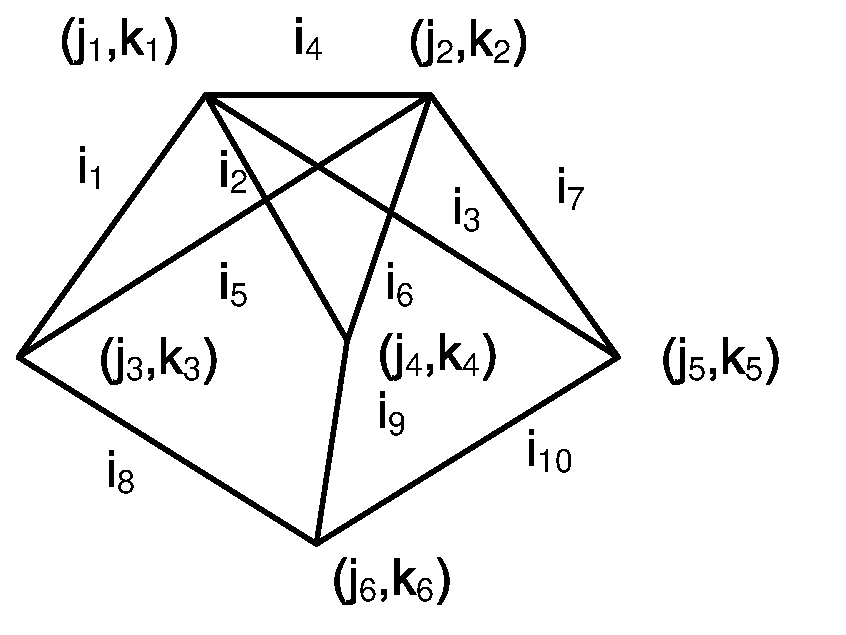
\includegraphics[width=3.2in,height=1.9in]{Drawing641_1.eps}
\caption{Depiction of the first candidate (6,4) set}\label{fig64a}
\end{figure}
\begin{figure}\center
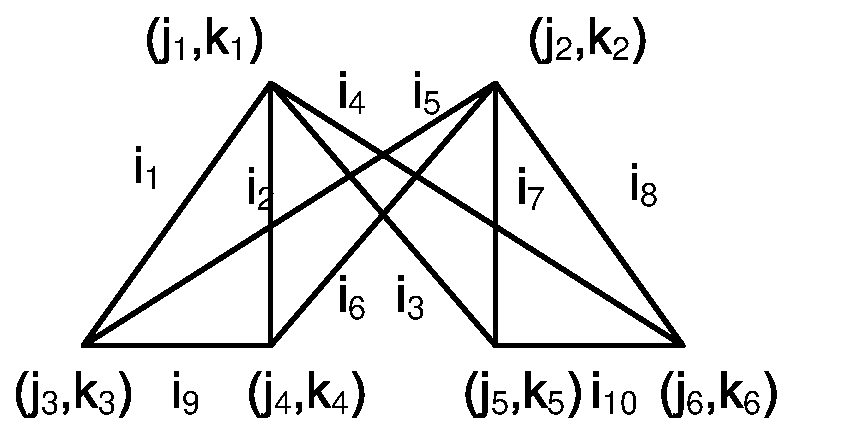
\includegraphics[width=3.2in,height=1.6in]{Drawing643_1.eps}
\caption{Depiction of the second candidate (6,4) set}\label{fig64b}
\end{figure}
\begin{figure}
\center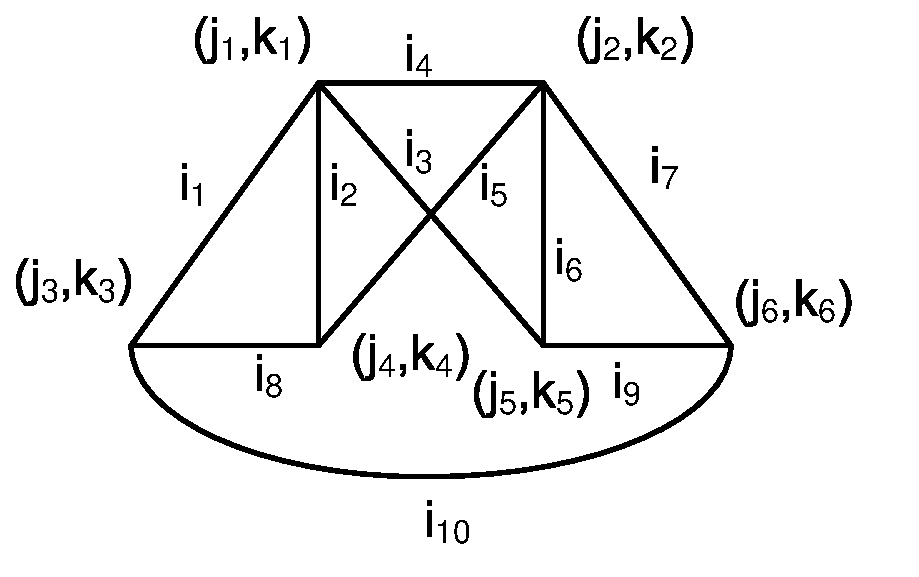
\includegraphics[width=3.2in,height=1.65in]{Drawing642_2.eps}
\caption{Depiction of the third candidate (6,4) set} \label{fig64c}
\end{figure}
%%%%%%%%%%%%%%%%%%%%%%%%%%%%%%%%%%%%%%%%%%%%%%%%%%%%%%%%%%%%%%%%%%%%
%XXXX figure plus analysis

By separately considering the cases when the two bit nodes that have
all neighboring checks satisfied have a satisfied check in common,
and the cases when they do not, one can show that there are 3
possible non isomorphic configurations, as shown in
Figure~\ref{fig64a},~\ref{fig64b}, and~\ref{fig64c}. By ensuring the
bit consistency, it further follows that for each configuration
there are 8 distinct edge labellings (as we show below).

Let us consider the topmost configuration first. The other two
configurations are analyzed subsequently.

\textbf{I. Candidate (6,4) configuration, given in Figure
~\ref{fig64a}.}

\comment{As before, we establish a congruential constraint for
each triplet consisting of an edge and its endpoints given in
Figure~\ref{fig64a}. The set of constraints consisting of 10 such
equations, one for each edge, is
\begin{eqnarray*}
k_1+i_1j_1 &\equiv& k_3+i_1j_3 \mod p, \\
k_1+i_2j_1 &\equiv& k_4+i_2j_4 \mod p,\\
k_1+i_3j_1 &\equiv& k_5+i_3j_5 \mod p, \\
k_1+i_4j_1 &\equiv& k_2+i_4j_2 \mod p, \\
k_2+i_5j_2 &\equiv& k_3+i_5j_3 \mod p, \\
k_2+i_6j_2 &\equiv& k_4+i_6j_4 \mod p, \\
k_2+i_7j_2 &\equiv& k_5+i_7j_5 \mod p, \\
k_3+i_8j_3 &\equiv& k_6+i_8j_6 \mod p, \\
k_4+i_9j_4 &\equiv& k_6+i_9j_6 \mod p,\text{and} \\
k_5+i_{10}j_5 &\equiv& k_6+i_{10}j_6 \mod p.
\end{eqnarray*}
}

We first determine all possible edge labellings. For convenience, we
assign $(i_1,i_2,i_3,i_4)$ $\asn$ $(x,y,z,w)$, where $x,y,z,w \in
\{0,1,2,3 \}$ and distinct by the bit consistency condition at
$(j_1,k_1)$. Then, by imposing the bit consistency conditions at
remaining vertices, the possible assignments for the remaining edge
labels are as follows
\begin{equation}\label{tuples}\begin{array}{cccccc} (i_5,i_6,i_7,i_8,i_9,i_{10}) \in
 \{(y,z,x,z,x,y), (z,x,y,y,z,x),  \\
 (y,z,x,z,w,y),
(y,z,x,w,x,y),  (y,z,x,z,x,w),\\(z,x,y,y,z,w)
(z,x,y,y,w,x),(z,x,y,w,z,x) \}. \end{array}\end{equation}
We first
observe that the assignments
$(i_1,i_2,i_3,i_4,i_5,i_6,i_7,i_8,i_9,i_{10})$
 = $(x,y,z,w,y,z,x,z,x,y)$ and
$(i_1,i_2,i_3,i_4,i_5,i_6,i_7,i_8,i_9,i_{10})$
=$(x,y,z,w,z,x,y,y,z,x)$ are in fact symmetric (exchange $y$ and
$z$) and is thus sufficient to analyze only one of them. Likewise,
by appealing to symmetry and after appropriate renamings, the
remaining six assignments also represent the same labelled
configuration. In particular, third and sixth assignments
in~\eqref{tuples} are symmetric,  as are fourth and seventh, and as
are fifth and eighth assignments. Fourth assignment follows from the
third by exchanging the labels $x$ and $y$, and the fifth assignment
follows from the third by exchanging the labels $x$ and $z$. It is
thus sufficient to consider only
$(i_1,i_2,i_3,i_4,i_5,i_6,i_7,i_8,i_9,i_{10})$=
$(x,y,z,w,y,z,x,z,x,y)$ or $(x,y,z,w,y,z,x,z,w,y)$.

Consider $(i_1,i_2,i_3,i_4,i_5,i_6,i_7,i_8,i_9,i_{10})$ =
$(x,y,z,w,y,z,x,z,x,y)$.

By applying the pattern consistency for each edge and its end points
in Figure~\ref{fig64a} we obtain
\begin{equation}\label{con64a}\begin{array}{cccc}
k_1+xj_1 &\equiv& k_3+xj_3 \mod p, \\
k_1+yj_1 &\equiv& k_4+yj_4 \mod p,\\
k_1+zj_1 &\equiv& k_5+zj_5 \mod p, \\
k_1+wj_1 &\equiv& k_2+wj_2 \mod p, \\
k_2+yj_2 &\equiv& k_3+yj_3 \mod p, \\
k_2+zj_2 &\equiv& k_4+zj_4 \mod p, \\
k_2+xj_2 &\equiv& k_5+xj_5 \mod p, \\
k_3+zj_3 &\equiv& k_6+zj_6 \mod p, \\
k_4+xj_4 &\equiv& k_6+xj_6 \mod p,\text{and} \\
k_5+yj_5 &\equiv& k_6+yj_6 \mod p.
\end{array}\end{equation}

Using the cycle consistency conditions for each of five cycles that
span the cycle space of the graph in Figure~\ref{fig64a} we also
write
\begin{equation}\label{con64b}\begin{array}{cccc}
w(j_2-j_1)+y(j_3-j_2)+x(j_1-j_3) \equiv 0 \mod p\\
w(j_2-j_1)+z(j_4-j_2)+y(j_1-j_4) \equiv 0 \mod p\\
w(j_2-j_1)+x(j_5-j_2)+z(j_1-j_5) \equiv 0 \mod p\\
y(j_4-j_1)+x(j_6-j_4)+z(j_3-j_6)+x(j_1-j_3) \equiv 0 \mod p\\
x(j_5-j_2)+y(j_6-j_5)+x(j_4-j_6)+z(j_2-j_4) \equiv 0 \mod p.
\end{array}\end{equation}


We will use the relationships in~\eqref{con64b} to express $j_3$
through $j_6$ in terms of $j_1$ and $(j_2-j_1)$, and then in turn
use~\eqref{con64a} to express $k_2 $ through $k_6$ in terms of
$k_1$, $j_1$ and $(j_2-j_1)$.


 By symmetry of the
configuration (see Figure~\ref{fig64a}), for the current labelling
it is sufficient to consider $x=0$ and $w=0$. Specifically,
letting $y=0$ or $z=0$ reduces to the $x=0$ case.

We let $a \asn j_2-j_1$, $b \asn j_3-j_1$, $c \asn j_4-j_1$,
 $d \asn j_5-j_1$, and $e \asn j_6-j_1$.  Note that in particular
 by the check consistency constraint, $a \neq 0$.

1. Case $x=0$.


The system in~\eqref{con64b} reduces to
 \begin{equation}\label{sys31aa}\begin{array}{ccccc}
 a(w-y)+by &\equiv 0 &\mod p\\
 a(z-w)+c(y-z)  &\equiv 0 &\mod p\\
 aw-dz &\equiv 0 &\mod p\\
 bz+yc-ze &\equiv 0 &\mod p\\
 az-cz-dy+ey &\equiv 0 &\mod p~.
 \end{array}
 \end{equation}

Using~\eqref{sys31aa} we express $b$, $c$ , $d$ and $e$ in terms of
$a$. In particular, the last constraint in~\eqref{sys31aa} is
redundant as it follows from the previous four, as we now show.

Express $b,c$ and $d$ of $a$ using top three  equations
in~\eqref{sys31aa} so that
\begin{equation}\begin{array}{llll}
b &\equiv& a \frac{y-w}{y} &\mod p \\
c &\equiv& a \frac{w-z}{y-z} &\mod p\\
d &\equiv& a \frac{w}{z} &\mod p~.
\end{array}
\end{equation}
Substitute for $b,c,d$ in terms of $a$ in the fourth equation of the
system~\eqref{sys31aa} to obtain \begin{equation}\label{eq1f} e
\equiv a (\frac{y-w}{y}-\frac{w-z}{y-z}\frac{y}{z}) \mod p~.
\end{equation}
Likewise, substitute for $b,c,d$ in terms of $a$ in the fifth
equation of the system \eqref{sys31aa} to obtain
\begin{equation}\label{eq2f} a\left(z-z\frac{w-z}{y-z}-\frac{wy}{z}
\right) +ey \equiv 0 \mod p~.
\end{equation}

From \eqref{eq1f} it follows that
\begin{equation}\label{eq3f}
(y-z)yze \equiv a \left( z(y-w)(y-z)+y^2(w-z) \right) \mod p,
\end{equation}
and from \eqref{eq2f} it follows that
\begin{equation}\label{eq4f}
a \left( z^2(y-z)-z^2(w-z)-wy(y-z) \right) +(y-z)yze \equiv 0 \mod
p~.
\end{equation}
Rewrite \eqref{eq4f} as
\begin{equation}\label{eq5f}
(y-z)yze \equiv a \left( -z^2(y-z)+z^2(w-z)+wy(y-z) \right)  \mod
p~.
\end{equation}
 We expand the terms that multiply $a$ in both \eqref{eq3f}
and \eqref{eq5f}. They both reduce to $-wyz-yz^2+wz^2+y^2w$, which
makes the last equation in the system \eqref{sys31aa} redundant.


Therefore, for $q \asn j_1$ and $t \asn j_2-j_1$, all of the
remaining values of $j_3,j_4,j_5,j_6$ follow for each of the $3!=6$
choices of $(y,z,w)$.

Using~\eqref{con64a} we further obtain
\begin{equation}\begin{array}{ccccc}
k_3 & \equiv& k_1 &\mod p\\
k_4 & \equiv& k_1-y(j_4-j_1) &\mod p\\
k_5 &\equiv& k_1-z(j_5-j_1) &\mod p\\
k_2 &\equiv& k_5 &\mod p\\
k_6 &\equiv& k_4 &\mod p. \end{array}\end{equation}

Therefore, we can express $k_2$ through $k_6$ in terms of $s \asn
k_1$, $q$ and $t$. The results for all choices of $(y,z,w)$ are
summarized in Table~\ref{table64}.

\hspace{-1in}\tiny{\begin{table*}[ht]\hspace{-1in}
\begin{tabular}{|c |c|c|c|c|c|c|c|c|c|c|c|c|c|}
  \hline
  % after \\: \hline or \cline{col1-col2} \cline{col3-col4} ...
  $y,z,w$ & $j_1$ & $j_2$ & $j_3$ & $j_4$ & $j_5$ & $j_6$ & $k_1$ & $k_2$ & $k_3$ & $k_4$ & $k_5$ & $k_6$ \\
  \hline
$3,2,1$&  $q$ & $q+t$ &  $q+\frac{2t}{3}$ &  $q-t$ & $q+\frac{t}{2}$
& $q-\frac{5t}{6}$ & $s$ & $s-t$ & $s$ & $s+3t$ & $s-t$ &
  $s+3t$\\
  $3,1,2$&$q$& $q+t$ &  $q+\frac{t}{3}$ &    $q+\frac{t}{2}$ &  $q+2t$ &   $q+\frac{11t}{6}$ & $s$ & $s-2t$ & $s$ & $s-\frac{3t}{2}$ & $s-2t$ &
  $s-\frac{3t}{2}$\\
 $2,3,1$& $q$ & $q+t$ &  $q+\frac{t}{2}$&    $q+2t$ &  $q+\frac{t}{3}$ &   $q+\frac{11t}{6}$ & $s$ & $s-t$ & $s$ & $s-4t$ & $s-t$ &
  $s-4t$\\
$2,1,3$&  $q$ & $q+t$ &  $q-\frac{t}{2}$ &  $q+2t$ &   $q+3t$ &
$q+\frac{7t}{2}$ & $s$ & $s-3t$ & $s$ & $s-4t$ & $s-3t$ &
  $s-8t$\\
 $1,2,3$& $q$ & $q+t$ &  $q-2t$ &    $q-t$ &    $q+\frac{3t}{2}$ &    $q-\frac{5t}{2}$ & $s$ & $s-3t$ & $s$ & $s+t$ & $s-3t$ &
  $s+t$\\
  $1,3,2$&$q$ & $q+t$ &  $q-t$ &    $q+\frac{t}{2}$ &  $q+\frac{2t}{3}$ &   $q-\frac{5t}{6}$ & $s$ & $s-2t$ & $s$ & $s-\frac{t}{2}$ & $s-2t$ &
  $s-\frac{t}{2}$\\
  \hline
\end{tabular}
\caption{ Several solution sets for the (6,4)
configuration.}\label{table64}
\end{table*}} \normalsize

\comment{[        q,      q+t,  q+2/3*t,      q-t,  q+1/2*t,
q-5/6*t, s, s-t,        s,    s+3*t,      s-t,    s+3*t]

[ q, q+t, q+1/3*t,  q+1/2*t,    q+2*t, q+11/6*t,        s,
s-2*t, s, s-3/2*t,    s-2*t,  s-3/2*t]

[        q,      q+t,  q+1/2*t, q+2*t,  q+1/3*t, q+11/6*t,
s,      s-t,        s,    s-4*t, s-t,    s-4*t]

[        q, q+t,  q-1/2*t,    q+2*t,    q+3*t, q+7/2*t,        s,
s-3*t, s,    s-4*t,    s-3*t, s-4*t]

[        q,      q+t, q-2*t, q-t,  q+3/2*t, q-5/2*t, s, s-3*t,
s,      s+t, s-3*t, s+t]

[        q, q+t, q-t, q+1/2*t,  q+2/3*t, q-5/6*t, s, s-2*t, s,
s-1/2*t, s-2*t, s-1/2*t]}
%file temp20.m

Furthermore, under the current configuration, the bit nodes in one
such $(6,4)$ absorbing set that have 3 satisfied and 1 unsatisfied
check, all have unsatisfied checks in the row group labelled $w$. By
the bit consistency condition, no bit node can connect to more than
one such check. Therefore, this configuration is in fact a $(6,4)$
fully absorbing set.

The (absolute) indices of columns that correspond to the bit nodes
in the absorbing set are $k_i+pj_i$ for $1 \leq i \leq 6$ and the
indices of rows that correspond to the unsatisfied check nodes in
the absorbing set are $(k_i+j_iw) \mod p+ wp$, for $3\leq i \leq
6$. In particular, the solution set in row 1 holds for all $p > 5$
and $t$ a multiple of $6$.

%%%% comment starts here
\comment{The system~\eqref{con64a} reduces to
\begin{equation}\begin{array}{ccccccccc}
k_1-k_3 &\equiv& 0 & {}& {}&{}&{}&\mod p
\\
k_2-k_5 &\equiv& 0 & {}& {}&{}&{}&\mod p
\\
k_4-k_6 &\equiv& 0 & {}& {}&{}&{}&\mod p
\\
k_1-k_4 &\equiv& y(j_4-j_1) &\equiv& z(j_6-j_3) &{}& {}&\mod p\\
k_2-k_4 &\equiv& z(j_4-j_2) & \equiv& y(j_6-j_5) &{} & {}&\mod p\\
 k_1-k_2 &\equiv& z(j_5-j_1) & \equiv& w(j_2-j_1) &\equiv& y(j_2-j_3)& \mod p~.
\end{array}\end{equation}


For convenience we let
\begin{equation}\label{eq29}\begin{array}{cccc}
k_1-k_4 &\equiv yzv &\mod p \\
k_1-k_2 &\equiv yzwt &\mod p\\
k_2-k_4 &\equiv yzs &\mod p,
\end{array}\end{equation}
for appropriately chosen integers $v,t$ and $s$.

From~\eqref{con64a} and~\eqref{eq29} we obtain
\begin{equation}\label{eq29a}\begin{array}{cccc}
\end{array}\end{equation}

We may express By fixing the values of $j_1$ and $t$, the rest of
$j_2$ through $j_6$ as well as $u$ and $s$ follow uniquely for
chosen $y,z$ and $w$ since based on the above we may write
\begin{equation}\label{eq30}
\left[ \begin{array}{ccccccc} 0 & 0 & 1 & 0 & 0 & -z &0\\
0 & 0 & 0 & 1 & 0 & 0 &0\\
1 & 0 & 0 & 0 & 0 & 0 &0\\
1 & -1 & 0 & 0 & 0 & 0 &0\\
-1 & 0 & 1 & 0 & 0 & 0 &-y\\
0 & -1 & 0 & 0 & 1 & -y &0\\
0 & 0 & 0 & -1 & 1 & 0 & -z
\end{array}\right] \left[\begin{array}{c}
j_2\\j_3\\j_4\\j_5\\j_6\\v\\s\end{array}\right] \equiv
\left[\begin{array}{c}j_1\\j_1+ywt\\j_1+yzt\\zwt\\0\\0\\0\end{array}\right]
\mod p~.
\end{equation}

Note that neither the vector multiplying the matrix nor the vector
on the right hand side cannot be an all-zeros vector as otherwise
the consistency conditions would be violated.

By inverting the matrix above, and using the relationships of these
variables with $k_1$ through $k_6$ we obtain the system of solutions
listed in Figure~\ref{table64}. As indicated, each row in the table
corresponds to a different numerical assignment of $y$, $z$ and $w$
(recall that $x=0$ for all six cases). In the table $q$, $t$ and $s$
are arbitrary residues $\mod p$ and the entries should be
interpreted $\mod p$. Note that we have thus established the
existence of $(6,4)$ absorbing sets. Moreover, the solutions for $s$
and $v$ obtained from \eqref{eq30} agree with \eqref{eq29}.

Furthermore, under the current configuration, the bit nodes in one
such $(6,4)$ absorbing set that have 3 satisfied and 1 unsatisfied
check, all have unsatisfied checks in the row group labelled $w$. By
the check consistency condition, no bit node can connect to more
than one such check. Therefore, this configuration is in fact a
$(6,4)$ fully absorbing set.

The (absolute) indices of columns that correspond to the bit nodes
in the absorbing set are $k_i+pj_i$ for $1 \leq i \leq 6$ and the
indices of rows that correspond to the unsatisfied check nodes in
the absorbing set are $(k_i+j_iw) \mod p+ wp$, for $3\leq i \leq 6$.
In particular, the solution set in row 1 holds for all $p > 5$.

\hspace{-0.95in}\small{\hspace{-0.95in}\begin{table*}[ht]\vspace{-0.05in}\hspace{-0.95in}
\begin{tabular}{|c |c|c|c|c|c|c|c|c|c|c|c|c|c|}
  \hline
  % after \\: \hline or \cline{col1-col2} \cline{col3-col4} ...
  $y,z,w$ & $j_1$ & $j_2$ & $j_3$ & $j_4$ & $j_5$ & $j_6$ & $k_1$ & $k_2$ & $k_3$ & $k_4$ & $k_5$ & $k_6$ \\
  \hline
$3,2,1$&  $q$ & $q+6t$ &  $q+4t$ &  $q-6t$ &  $q+3t$ & $q-5t$ & $s$
& $s-6t$ & $s$ & $s+18t$ & $s-6t$ &
  $s+18t$\\
  $3,1,2$&$q$& $q+3t$ &  $q+t$ &    $q+\frac{3t}{2}$ &  $q+6t$ &   $q+\frac{11t}{2}$ & $s$ & $s-6t$ & $s$ & $s-\frac{9t}{2}$ & $s-6t$ &
  $s-\frac{9t}{2}$\\
 $2,3,1$& $q$ & $q+6t$ &  $q+3t$&    $q+12t$ &  $q+2t$ &   $q+11t$ & $s$ & $s-6t$ & $s$ & $s-24t$ & $s-6t$ &
  $s-24t$\\
$2,1,3$&  $q$ & $q+2t$ &  $q-t$ &  $q+4t$ &   $q+6t$ &    $q+7t$ &
$s$ & $s-6t$ & $s$ & $s-8t$ & $s-6t$ &
  $s-8t$\\
 $1,2,3$& $q$ & $q+2t$ &  $q-4t$ &    $q-2t$ &    $q+3t$ &    $q-5t$ & $s$ & $s-6t$ & $s$ & $s+2t$ & $s-6t$ &
  $s+2t$\\
  $1,3,2$&$q$ & $q+3t$ &  $q-3t$ &    $q+3/2t$ &  $q+2t$ &   $q-5/2t$ & $s$ & $s-6t$ & $s$ & $s-3/2t$ & $s-6t$ &
  $s-3/2t$\\
  \hline
\end{tabular}
\caption{ Several solution sets for the (6,4)
configuration.}\label{table64}
\end{table*}}
\normalsize }
%\textbf{comment on s and u being consistent} \textbf{comment on
%singularity}
%%%%% comment ends here

We complete the analysis of this label assignment by considering
$w=0$.

2. Case $w=0$



In this case the system in~\eqref{con64b} reduces to:
 \begin{equation}\label{sys31a}\begin{array}{ccccc}
 ay+b(x-y) &\equiv 0 &\mod p\\
 az+c(y-z)  &\equiv 0 &\mod p\\
 ax+d(z-x) &\equiv 0 &\mod p\\
 b(z-x)+c(y-x)+e(x-z) &\equiv 0 &\mod p\\
 a(z-x)+c(x-z)+d(x-y)+e(y-x) &\equiv 0 &\mod p~.
 \end{array}
 \end{equation}


Note that the last relation follows from the previous four. We again
express $b$, $c$ $d$ and $e$ in terms of $a$, so that by setting
$j_1 \asn q$ and $a \asn t$, all of $j_2$ through $j_6$ follow as a
function of $q$ and $t$. Then, by letting $k_1 \asn s$, the
remaining $k_2$ through $k_6$ follow from $q,t$ and $s$
from~\eqref{con64a}. The solution set for various numerical
assignments of $(x,y,z)$ is given in Table~\ref{table641}.
\hspace{-0.95in}\small{\hspace{-0.95in}\begin{table*}[ht]\vspace{-0.05in}\hspace{-0.95in}
\begin{tabular}{|c |c|c|c|c|c|c|c|c|c|c|c|c|c|}
  \hline
  % after \\: \hline or \cline{col1-col2} \cline{col3-col4} ...
  $x,y,z$ & $j_1$ & $j_2$ & $j_3$ & $j_4$ & $j_5$ & $j_6$ & $k_1$ & $k_2$ & $k_3$ & $k_4$ & $k_5$ & $k_6$ \\
  \hline
    $3,2,1$ & $q$ &$q+t$ & $q-2t$ & $q-t$& $q+\frac{3t}{2}$ &$q-\frac{5t}{2}$ & $s$ &$s$ &   $s+6t$ & $s+2t$ & $s-\frac{3t}{2}$ &
    $s+\frac{13t}{2}$\\
     $3,1,2$ & $q$ &$q+t$ & $q-\frac{t}{2}$ & $q+2t$& $q+3t$ &$q+\frac{7t}{2}$ & $s$ &$s$ &   $s+\frac{3t}{2}$ & $s-2t$ & $s-6t$ &
    $s-\frac{13t}{2}$\\
     $2,3,1$ & $q$ &$q+t$ & $q+3t$ & $q-\frac{t}{2}$& $q+2t$ &$q+\frac{7t}{2}$ & $s$ &$s$ &   $s-6t$ & $s+\frac{3t}{2}$ & $s-2t$ &
    $s-\frac{13t}{2}$\\
     $2,1,3$ & $q$ &$q+t$ & $q-t$ & $q+\frac{3t}{2}$& $q-2t$ &$q-\frac{5t}{2}$ & $s$ &$s$ &   $s+2t$ & $s-\frac{3t}{2}$ & $s+6t$ &
    $s+\frac{13t}{2}$\\
     $1,2,3$ & $q$ &$q+t$ & $q+2t$ & $q+3t$& $q-\frac{t}{2}$ &$q+\frac{7t}{2}$ & $s$ &$s$ &   $s-2t$ & $s-6t$ & $s+\frac{3t}{2}$ &
    $s-\frac{13t}{2}$\\
     $1,3,2$ & $q$ &$q+t$ & $q+\frac{3t}{2}$ & $q-2t$& $q-t$ &$q-\frac{5t}{2}$ & $s$ &$s$ &   $s-\frac{3t}{2}$ & $s+6t$ & $s+2t$ &
    $s+\frac{13t}{2}$\\
  \hline
\end{tabular}
\caption{ Several solution sets for the (6,4)
configuration.}\label{table641}
\end{table*}}
\normalsize %\textbf{comment on fully absorbing sets}
%%%% this is in temp16.m
 \comment{    [        q,      q+t, q-2*t,
q-t, q+3/2*t, q-5/2*t, s,        s,    s+6*t,    s+2*t, s-3/2*t,
s+13/2*t] [ q, q+t,  q-1/2*t,    q+2*t,    q+3*t, q+7/2*t, s, s,
s+3/2*t, s-2*t,    s-6*t, s-13/2*t] [        q, q+t,    q+3*t,
q-1/2*t, q+2*t,  q+7/2*t,        s,        s, s-6*t,  s+3/2*t,
s-2*t, s-13/2*t] [        q,      q+t, q-t, q+3/2*t,    q-2*t,
q-5/2*t, s,        s,    s+2*t, s-3/2*t, s+6*t, s+13/2*t] [ q,
q+t,    q+2*t, q+3*t,  q-1/2*t, q+7/2*t, s, s, s-2*t, s-6*t,
s+3/2*t, s-13/2*t] [        q, q+t, q+3/2*t, q-2*t, q-t, q-5/2*t,
s,        s,  s-3/2*t, s+6*t, s+2*t, s+13/2*t] }


As in the $x=0$ case, the unsatisfied checks all belong in the row
group labelled $w$. By the bit consistency condition, no bit node
can connect to more than one such check. Therefore, this
configuration is also in fact a $(6,4)$ fully absorbing set.

The (absolute) indices of columns that correspond to the bit nodes
in the absorbing set are $k_i+pj_i$ for $1 \leq i \leq 6$ and the
indices of rows that correspond to the unsatisfied check nodes in
the absorbing set are $(k_i+j_iw) \mod p+ wp$, for $3\leq i \leq 6$.
In particular, the solution set in row 1 of the table in
Figure~\ref{table641} holds for all $p
> 5$ and $t$ even.


 The remaining labelled configuration of Figure~\ref{fig64a} to be considered is
\newline \noindent$(i_1,i_2,i_3,i_4,i_5,i_6,i_7,i_8,i_9,i_{10})$ =
$(x,y,z,w,y,z,x,z,w,y)$.

We let $a \asn j_2-j_1$, $b \asn j_3-j_1$, $c \asn j_4-j_1$,
 $d \asn j_5-j_1$, and $e \asn j_6-j_1$.  Note that in particular
 by the check consistency constraint, $a \neq 0$.

Based on the cycles consistency condition for the five cycles in
Figure~\ref{fig64a} we establish
 \begin{equation}\label{sys31}\begin{array}{cccc}
 a(w-y)+b(y-x) &\equiv 0 &\mod p\\
 a(w-z)+c(z-y) &\equiv 0 &\mod p\\
 a(w-x)+d(x-z) &\equiv 0 &\mod p\\
 c(y-w)+b(z-x)+e(w-z) &\equiv 0 &\mod p\\
 d(x-y)+a(z-x)+c(w-z)+e(y-w)&\equiv 0 &\mod p~.
 \end{array}
 \end{equation}



By expressing $b$, $c$ and $d$ in terms of $a$, from this system
we obtain
\begin{eqnarray}\label{sys32a}
a\left(\frac{(y-w)(w-z)}{y-z}+\frac{(z-x)(w-y)}{x-y} \right)+e(w-z) &\equiv 0 &\mod p\\
\label{sys32b}a\left(\frac{(x-y)(w-x)}{z-x}+(z-x)+\frac{(w-z)^2}{y-z}
\right)+e(y-w)&\equiv 0 &\mod p,
\end{eqnarray}
where $\{x,y,z,w\} =\{0,1,2,3\}$ and are distinct. For all $4!=24$
distinct ways of assigning numerical values to $x,y,z$ and $w$, the
system \eqref{sys32a}--\eqref{sys32b} produces the unique solution
$a=0$, $e=0$, provided that $p>3$. Since $a\neq 0$ by the check
consistency condition, we conclude that this configuration is not
possible.

\comment{temp5.m and temp6.m and temp7.m which are superseded by
temp15.m} \comment{temp14.m and temp15.m} %\textbf{put this first}

We now consider the second candidate (6,4) configuration.

\textbf{II. Candidate (6,4) configuration, given in Figure
~\ref{fig64b}.}

We first determine all possible edge labellings. For convenience,
let $(i_1,i_2,i_3,i_4)$ $\asn$ $(x,y,z,w)$, where $x,y,z,w \in
\{0,1,2,3 \}$ and are distinct by the bit consistency condition at
$(j_1,k_1)$. Then, by imposing the bit consistency conditions at
remaining vertices, the assignments for the remaining edge labels
are given by the following set
\begin{equation}\label{tuples2}\begin{array}{cccc} (i_5,i_6,i_7,i_8,i_9,i_{10}) \in
 \{(y,x,w,z,z,x),(w,x,y,z,z,x),\\
 (y,x,w,z,z,y),(y,w,x,z,z,y),(y,x,w,z,w,x),\\(z,x,w,y,w,x),(y,z,w,x,w,y),(y,x,w,z,w,y)\}~.
\end{array}\end{equation}

Out of these 8 possible labelled configurations by appealing to
symmetry and label renaming it is sufficient to consider only 2 of
these as we now show. Note that the eighth labelling is the same
as the first labelling after we exchange $(j_3,k_3)$ and
$(j_4,k_4)$, $(j_5,k_5)$ and $(j_6,k_6)$, and labels $y$ with $x$
and $w$ with $z$. Likewise, the second labelling is the same as
the seventh labelling after we exchange $(j_3,k_3)$ and
$(j_4,k_4)$, $(j_5,k_5)$ and $(j_6,k_6)$, and labels $y$ with $x$
and $w$ with $z$. Sixth labelling is the same as the fourth
labelling after we exchange labels $z$ with $x$, $y$ with $w$, and
nodes $(j_1,k_1)$ with $(j_2,k_2)$, $(j_3,k_3)$ with $(j_4,k_4)$,
and $(j_5,k_5)$ with $(j_6,k_6)$, and take the mirror image of the
resulting configuration. Fifth labelling is the same as the third
after we exchange labels $z$ with $x$ and $y$ with $w$ and take
the mirror image of the whole configuration. Fourth (respectively
first) labelling is the same as the second (respectively third)
after we exchange $(j_3,k_3)$ and $(j_4,k_4)$ and labels $x$ and
$y$.

It is thus sufficient to consider only two different labellings,
namely \newline
\noindent$(i_1,i_2,i_3,i_4,i_5,i_6,i_7,i_8,i_9,i_{10})$=
$(x,y,z,w,y,x,w,z,z,y)$ (third labelling) and
\newline \noindent $(i_1,i_2,i_3,i_4,i_5,i_6,i_7,i_8,i_9,i_{10})$ =
$(x,y,z,w,y,z,w,x,w,y)$ (seventh labelling).

For the first remaining case, by symmetry, it is sufficient to
consider $x=0$ and $z=0$ as $w=0$ and $y=0$ reduce to the $x=0$
and $z=0$ case respectively. Likewise, for the second case it is
sufficient to consider $x=0$ and $y=0$, as $z=0$ and $w=0$ each
reduce to the $x=0$ and $y=0$ cases, respectively.

%Let us consider $(i_1,i_2,i_3,i_4,i_5,i_6,i_7,i_8,i_9,i_{10})$=
%$(x,y,z,w,y,x,w,z,z,y)$ first, with $x=0$.




%We now consider $(i_1,i_2,i_3,i_4,i_5,i_6,i_7,i_8,i_9,i_{10})$=
%$(x,y,z,w,y,x,w,z,z,y)$ first, starting with with $z=0$. \comment{
%Consider $z=0$ XXXXXXXXXXX-6 THIS IS DONE. HAS ONE VALID
% SOLUTION. SEE TEMP2.M}

Consider $(i_1,i_2,i_3,i_4,i_5,i_6,i_7,i_8,i_9,i_{10})$=
$(x,y,z,w,y,x,w,z,z,y)$.

1. Case $z=0$

 From Figure~\ref{fig64b} and under the current edge label
 assignment using the pattern consistency constraints of Corollary~\ref{patterncor} we write
\begin{equation}\label{eq10a}\begin{array}{ccccc}
k_1 & \equiv &k_5 &\mod p\\
k_2 & \equiv &k_6 &\mod p\\
k_3 & \equiv &k_4 &\mod p\\
k_1+xj_1 & \equiv & k_3+xj_3 &\mod p\\
k_1+yj_1 & \equiv & k_4+yj_4 &\mod p\\
k_1+wj_1 & \equiv & k_6+wj_6 &\mod p\\
k_2+yj_2 & \equiv & k_3+yj_3 &\mod p\\
k_2+xj_2 & \equiv & k_4+xj_4 &\mod p\\
k_2+wj_2 & \equiv & k_5+wj_5 &\mod p\\
k_5+yj_5 & \equiv & k_6+yj_6 &\mod p~.
\end{array}\end{equation}

\comment{From \eqref{eq10a} we write
\begin{equation}\label{eq10b}\begin{array}{cccc}
k_2-k_3 &\equiv xyv &\mod p \\
k_1-k_2 &\equiv ywt &\mod p\\
k_1-k_3 &\equiv xys &\mod p,
\end{array}\end{equation}
for appropriately chosen integers $v,t$ and $s$. Note that by the
check consistency condition all of $v,t$ and $s$ are non zero
residues $\mod p$.


We now express $j_2$ through $j_6$, $s$ and $v$ in terms of $j_1$
and $t$ based on \eqref{eq10a} and \eqref{eq10b}, as
\begin{equation}\label{eq10c}
\left[ \begin{array}{ccccccc} 0 & 0 & 0 & 0 & 1 & 0 &0\\
1 & 0 & 0 & -1 & 0 & 0 &0\\
0 & 0 & 0 & -1 & 1 & 0 &0\\
0 & 1 & 0 & 0 & 0 & -y &0\\
0 & 0 & 1 & 0 & 0 & -x &0\\
-1 & 1 & 0 & 0 & 0 & 0 &-x\\
-1 & 0 & 1 & 0 & 0 & 0 &-y
\end{array}\right] \left[\begin{array}{c}
j_2\\j_3\\j_4\\j_5\\j_6\\s\\v\end{array}\right] \equiv
\left[\begin{array}{c}j_1+yt\\yt\\wt\\j_1\\j_1\\0\\0\end{array}\right]
\mod p~.
\end{equation}

Note that neither the vector multiplying the matrix nor the vector
on the right hand side can be an all-zeros vector as otherwise the
consistency conditions would be violated.

In all $3!=6$ choices for $(x,y,w)$, the solution for $s$ and $v$ to
\eqref{eq10c} expresses them as multiples of $t$. Since $wt \equiv
x(s-v) \mod p$ (write $k_1-k_2$ as $(k_1-k_3)-(k_2-k_3)$), in all
but one of these solutions, it then follows that $t \equiv 0 \mod p$
for $p>7$, which violates the check consistency condition. The
remaining case (when $t$ is a non zero residue) corresponds to
$x=1$, $y=3$, and $w=2$ for which we establish the solution set
listed in Table~\ref{table64b} for $j_1=q$ and $k_1=s$.}%%% end comment


Let $a\asn j_2-j_1$, $b\asn j_3-j_1$, $c\asn j_4-j_1$, $d\asn
j_5-j_1$ and $e\asn j_6-j_1$. Using the cycle constraint for  four
cycles spanning the cycle space of the configuration in
Figure~\ref{fig64b} and under the current edge labelling we have
\begin{equation}\label{eq1}\begin{array}{cccc}
xb+y(-c) &\equiv &0 \mod p, \\
y(b-a)+x(a-c) &\equiv &0 \mod p, \\
y(e-d) +w(-e) &\equiv &0 \mod p, \\
w(d-a)+y(e-d)&\equiv &0 \mod p .\end{array}\end{equation}
From the
system~\eqref{eq10a} we write
\begin{equation}\label{eq2}\begin{array}{lll}
k_1 -k_2 \equiv k_1-k_6 \equiv w(j_6-j_1) \equiv we &\mod p,\\
k_1-k_3 \equiv k_1 -k_4 \equiv y(j_4-j_1) \equiv yc &\mod p,\\
k_2 -k_3 \equiv y(j_3-j_2) \equiv y(b-a) &\mod p.
\end{array}\end{equation}
Using the identity $(k_1-k_2)=(k_1-k_3)-(k_2-k_3)$, and \eqref{eq2}
we obtain
\begin{equation}\label{eq3}
we \equiv y(c-b+a) \mod p.
\end{equation}

There are six possible assignments for $(x,y,w)$, as permutations of
the set $(1,2,3)$. In the remainder we will show that in fact only
$(x,y,w)=(1,3,2)$ gives rise to absorbing sets. In all other cases,
using \eqref{eq1} and \eqref{eq3}, we will reach a contradiction.

From \eqref{eq1} we have
\begin{equation}\label{eq4}\begin{array}{ccc}
xb \equiv yc \mod p\\
yd \equiv (y-w)e \mod p.
\end{array}\end{equation}
We also have
\begin{equation}\label{eq5}\begin{array}{ccc}
xa -(y+x)c \equiv 0 \mod p\\
(2y-w)e \equiv ya \mod p,
\end{array}\end{equation}

where the top expression in \eqref{eq5} follows from substituting
top expression in \eqref{eq4} into the second expression of
\eqref{eq1} and the bottom expression in \eqref{eq5} follows from
substituting bottom expression in \eqref{eq4} into the fourth
expression of \eqref{eq1}.

For $(y,w,x)=(1,2,3)$, the bottom expression in \eqref{eq5} gives
\[
a \equiv 0 \mod p,\\
\]
which then implies
\[
c\equiv 0 \mod p,\\
\]
by the top expression in \eqref{eq5}. Since $c=j_4-j_1$, and
$(j_1,k_1)$ and $(j_4,k_4)$ share a check, $c$ must be non-zero,
implying a contradiction.

For $(y,w,x) \in \{ (1,3,2), (2,1,3), (2,3,1),(3,1,2)\}$ we express
$b,c,d,e$ in terms of $a$ using \eqref{eq4} and \eqref{eq5}.

For $(y,w,x)=(1,3,2)$ we obtain: \[b \equiv a/3 \mod p, c \equiv2a/3
\mod p, d \equiv 2a \mod p, e \equiv -a \mod p.\]

For $(y,w,x)=(2,1,3)$ we obtain: \[b \equiv 2a/5 \mod p, c \equiv
3a/5 \mod p, d \equiv a/3 \mod p, e \equiv 2a/3 \mod p.\]

For $(y,w,x)=(2,3,1)$ we obtain: \[b \equiv 2a/3 \mod p, c \equiv
a/3 \mod p, d \equiv -a \mod p, e \equiv 2a \mod p.\]

For $(y,w,x)=(3,1,2)$ we obtain: \[b \equiv 3a/5 \mod p, c \equiv
2a/5 \mod p, d \equiv 2a/5 \mod p, e \equiv 3a/5 \mod p.\]

In all four cases, when $b,c$ and $e$ are substituted in \eqref{eq3}
it follows that $a \equiv 0 \mod p$ (we get $-3a \equiv 4a/3 \mod
p$, $2a/3 \equiv 12a/5 \mod p$, $6a \equiv 4a/3 \mod p$, and $3a/5
\equiv 12a/5 \mod p$, respectively). Since $b$ is a multiple of $a$
in all four cases, if $a \equiv 0 \mod p$, then $b \equiv 0 \mod p$
as well. Since $b=j_3-j_1$ and nodes $(j_1,k_1)$ and $(j_3,k_3)$
share a check, $b$ must be non-zero, thus implying a contradiction.

For $(y,w,x)=(3,2,1)$ we obtain: \[b \equiv 3a/4 \mod p, c \equiv
a/4 \mod p, d \equiv a/4 \mod p, e \equiv 3a/4 \mod p.\] When $b,c$
and $e$ are substituted in \eqref{eq3}, we obtain the identity $3a/2
\equiv 3a/2 \mod p$. Since $c \equiv d \mod p$, we have that
$j_4=j_5$ and since $b \equiv e \mod p$, we have that $j_3=j_6$.
Note that neither of these two conditions on $j$s violates the check
consistency constraint since the respective bit nodes do not share a
check in Figure 12. Let $q=j_1$ and $t=j_4 -j_1$. Then $j_4=q+t$ and
$j_5=q+t$. Since $b=3c$, and $b=j_3-j_1$ and $c=j_4-j_1$, we have
that $j_3=q+3t$. Since $j_3=j_6$, $j_6=q+3t$ as well. Likewise,
since $a=4c$, and $a=j_2-j_1$ and $c=j_4-j_1$, we have that
$j_2=q+4t$. We have thus expressed all of $j_1$ through $j_6$ in
terms of $q$ and $t$. Now the system~\eqref{eq10a} reduces to
\begin{equation}\label{eq6}\begin{array}{ccc}
k_1 &\equiv& k_5 \mod p,\\
k_2 &\equiv& k_6 \mod p,\\
k_3 &\equiv& k_4 \mod p,\\
k_1 -k_3 &\equiv& 3t \mod p,\\
k_1 -k_2 &\equiv& 6t \mod p,\\
k_2 -k_3 &\equiv& -3t \mod p.\\
\end{array}\end{equation}

Thus, with $s=k_1$ and using \eqref{eq6} we can express all of $k_1$
through $k_6$ in terms of $s$ and $t$. This solution set for $j_1$
through $j_6$ and $k_1$ through $k_6$ is listed in
Table~\ref{table64b}.

\hspace{-0.2in}\small{\hspace{-0.2in}\begin{table*}[ht]\vspace{-0.05in}\hspace{-0.2in}
\begin{tabular}{|c |c|c|c|c|c|c|c|c|c|c|c|c|c|}
  % after \\: \hline or \cline{col1-col2} \cline{col3-col4} ...
  \hline
  $x,y,w$ & $j_1$ & $j_2$ & $j_3$ & $j_4$ & $j_5$ & $j_6$ & $k_1$ & $k_2$ & $k_3$ & $k_4$ & $k_5$ & $k_6$ \\
  \hline
$1,3,2$&  $q$ & $q+4t$ &  $q+3t$ &  $q+t$ &  $q+t$ & $q+3t$ & $s$ &
$s-6t$ & $s-3t$ & $s-3t$ & $s$ &
  $s-6t$\\
  \hline
\end{tabular}
\caption{ A solution set for an (6,4) absorbing
set.}\label{table64b}
\end{table*}}
\normalsize

Note that the result in Table~\ref{table64b} establishes the
existence of a (6,4) absorbing set. Even though $j_3=j_6$ and
$j_4=j_5$ the check consistency constraints are not violated as
$(j_3,k_3)$ and $(j_6,k_6)$ do not share an edge, and neither do
$(j_4,k_4)$ and $(j_5,k_5)$, see Figure~\ref{fig64b}.

 We now discuss whether this set is
also a (6,4) fully absorbing set. Suppose there exists a bit node
$(j_7,k_7)$ outside this absorbing set that is incident to some of
the unsatisfied checks. By the bit consistency constraint, both
$(j_3,k_3)$ and $(j_4,k_4)$ each have a neighboring unsatisfied
check whose label is $w$. These two checks must be distinct by the
girth condition. Likewise, both $(j_5,k_5)$ and $(j_6,k_6)$ each
have a neighboring unsatisfied check whose label is $x$, and these
are also distinct by the girth condition. By the bit consistency
condition, the bit node $(j_7,k_7)$ can then share at most 2 of
these checks with the bit nodes $(j_3,k_3)$ through $(j_7,k_7)$.

Suppose that the bit node $(j_7,k_7)$ shares the check with each
of $(j_3,k_3)$ and $(j_5,k_5)$. From the cycles relating bit nodes
$(j_7,k_7)$, $(j_3,k_3)$, $(j_5,k_5)$, $(j_1,k_1)$, and
$(j_2,k_2)$, we obtain
\begin{eqnarray*}
x(j_7-j_5)+w(j_3-j_7)+x(j_1-j_3) &\equiv 0& \mod p\\
w(j_5-j_2)+x(j_7-j_5)+w(j_3-j_7)+y(j_2-j_3) &\equiv 0& \mod p~.
\end{eqnarray*}

For $(x,y,z,w)=(1,3,0,2)$ of present interest, we obtain that $j_7
\equiv q+2t \mod p$ using the result in Table~\ref{table64b}.

Since we further have
\begin{eqnarray*}
k_3+2j_3 &\equiv & k_7+2j_7 \mod p\\
k_5+j_5 & \equiv & k_7 +j_7 \mod p,
\end{eqnarray*}
it follows that $k_7 \equiv s-t \mod p$. Therefore by the existence
of this bit node $(j_7,k_7)$, the current (6,4) absorbing set is not
a (6,4) fully absorbing set.

%%% comment on other choices.

%%% in temp23.m using cycles

%%%%%%%%%%%%%%%%%%%%%%%%%%%%%%%%%%%%%%%%%%%%%%
%\textbf{comment on fully absorbing sets}

 We now consider
$(i_1,i_2,i_3,i_4,i_5,i_6,i_7,i_8,i_9,i_{10})$=
$(x,y,z,w,y,x,w,z,z,y)$ with $x=0$. \comment{Consider $x=0$
XXXXXXXXXXX=5 THIS IS DONE. VALID SOLS FOR 213 AND 231 IN TERMS OF
J1 AND K1}

1. Case $x=0$

As before, using the pattern consistency constraints we establish:
\begin{equation}\label{eq11c}\begin{array}{cccc}
k_1 & \equiv & k_3 \mod p\\
k_2 & \equiv & k_4 \mod p\\
k_1+yj_1 & \equiv & k_4+yj_4 \mod p\\
k_1+zj_1 & \equiv & k_5+zj_5 \mod p\\
k_1+wj_1 & \equiv & k_6+wj_6 \mod p\\
k_2+yj_2 & \equiv & k_3+yj_3 \mod p\\
k_2+wj_2 & \equiv & k_5+wj_5 \mod p\\
k_2+zj_2 & \equiv & k_6+zj_6 \mod p\\
k_3+zj_3 & \equiv & k_4+zj_4 \mod p\\
k_5+yj_5 & \equiv & k_6+yj_6 \mod p,~.
\end{array}\end{equation}

Let $a \asn j_2 -j_1$, $b \asn j_3 -j_1$, $c \asn j_4 -j_1$, $d \asn
j_5 -j_1$, and $e \asn j_6 -j_1$. Using the cycle constraints for
four cycles spanning the cycle space of the configuration in
Figure~\ref{fig64b} we may also write
\begin{equation}\label{eq11d}\begin{array}{cccc}
z(c-b)+y(-c) &\equiv & 0 \mod p, \\
y(b-a)+z(c-b)&\equiv & 0 \mod p, \\
zd+y(e-d)+w(-e) &\equiv & 0 \mod p, \\
w(d-a)+y(e-d)+z(a-e) &\equiv & 0 \mod p~.
\end{array}\end{equation}


There are 6 possible assignments for $(y,z,w)$ as permutations of
the set $\{1,2,3\}$. We will show that in fact the only possible
assignment is $(y,z,w)=(2,1,3)$ (a contradiction will be reached
in all other cases).

Consider first the assignment $(y,z,w)=(1,2,3)$.
Using~\eqref{eq11d} we express $a$, $b$, $c$ and $d$ in terms of
$e$ so that
\begin{equation}\label{eq11e}\begin{array}{cccc}
a &\equiv & 3e \mod p, \\
b &\equiv & e \mod p, \\
c &\equiv & 2e \mod p, \\
d &\equiv & 2e \mod p~. \\
\end{array}\end{equation}

Note that since $c \equiv d \mod p$ and  $b \equiv e \mod p$ the
above implies that $j_4=j_5$ and $j_3=j_6$. Even though now some
vertices have the same $j$ components, the check consistency
condition is not violated as $(j_4,k_4)$ and $(j_5,k_5)$ do not
share an edge, and neither do $(j_3,k_3)$ and $(j_6,k_6)$ (see
Figure~\ref{fig64b}).

From~\eqref{eq11c} and by substituting for $a$, $c$ and $d$ in
terms of $e$ using~\eqref{eq11e} we note that
\begin{equation}\label{eq11f}\begin{array}{cccc}
k_1-k_2 \equiv 1(2e) \mod p, \\
k_1-k_5 \equiv 2(2e) \mod p, \\
k_2-k_5 \equiv 3(2e-3e) \mod p~.
\end{array}\end{equation}

The system~\eqref{eq11f} implies that $e \equiv 0 \mod p$ for $p>5$.
Since $e=j_6-j_1$ and $(j_1,k_1)$ and $(j_6,k_6)$ do share an edge,
the condition $e \equiv 0 \mod p$ violates the check consistency
constraint. We thus conclude that the current numerical assignment
for $(y,z,w)$ is not possible.

By expressing $a$, $b$, $c$ and $d$ in terms of $e$ as
in~\eqref{eq11e} and then using~\eqref{eq11c} to express the
differences $k_1-k_2$, $k_1-k_5$, and $k_2-k_5$ as
in~\eqref{eq11f} we conclude that $e \equiv 0 \mod p$ when
$(y,z,w)$ = $(1,3,2)$ and $p>5$ as well as $(y,z,w)$ = $(3,1,2)$
and $p>7$ or $(3,2,1)$ and $p>13$.

Consider now the assignment $(y,z,w)=(2,3,1)$. Using~\eqref{eq11d}
it follows after substituting for $d$ in terms of $e$ in the last
expression that
\begin{eqnarray}
a \equiv 0 \mod p~.
\end{eqnarray}
By substituting for $b$ in terms of $c$ in the second expression
in~\eqref{eq11d} it also follows that
\begin{eqnarray}
3a \equiv 4c \mod p~.
\end{eqnarray}
Therefore $c \equiv 0 \mod p$, which violates the check consistency
constraint for the edge connecting bit nodes $(j_1,k_1)$ and
$(j_4,k_4)$. The condition $a \equiv 0 \mod p$ by itself does not
yield a contradiction as the nodes $(j_1,k_1)$ and $(j_2,k_2)$ do
not have any edges in common.

Finally, we consider the assignment $(y,z,w)=(2,1,3)$. First, by
substituting for $d$ in terms of $e$ in the last expression that
\begin{eqnarray}
a \equiv 0 \mod p~.
\end{eqnarray}
Therefore $j_1=j_2$. By substituting for $b$ in terms of $c$ in
the second expression in~\eqref{eq11d} we have that
\begin{eqnarray}
1a \equiv (2-2)c \mod p~,
\end{eqnarray}
which does not tell us anything about the actual value of $c$. We
express $b$, $c$ and $d$ in terms of $e$, again
using~\eqref{eq11d}, and obtain
\begin{equation}\label{eq11g}\begin{array}{cccc}
b &\equiv & -e \mod p, \\
c &\equiv & e \mod p, \\
d &\equiv & -e \mod p~. \\
\end{array}\end{equation}
Since $b \equiv d \mod p$, $j_3=j_5$, and since $c \equiv e \mod p$,
$j_4=j_6$. Neither of these conditions on $j$'s violates the check
consistency constraints as the respective bit nodes do not share
edges (see Figure~\ref{fig64b}). Thus, with $q \asn j_1$ and $t \asn
e$ we can express all of $j_1$ through $j_6$ in terms of $q$ and
$t$. Having verified that all constraints given by~\eqref{eq11c} are
in fact consistent for $s \asn k_1$ we obtain the solution set given
in Table ~\ref{table64c}, in terms of $q,t$ and $s$.

\hspace{-0.2in}\small{\hspace{-0.2in}\begin{table*}[ht]\vspace{-0.05in}\hspace{-0.2in}
\begin{tabular}{|c |c|c|c|c|c|c|c|c|c|c|c|c|c|}
  % after \\: \hline or \cline{col1-col2} \cline{col3-col4} ...
  \hline
  $y,z,w$ & $j_1$ & $j_2$ & $j_3$ & $j_4$ & $j_5$ & $j_6$ & $k_1$ & $k_2$ & $k_3$ & $k_4$ & $k_5$ & $k_6$ \\
  \hline
$2,1,3$&  $q$ & $q$ &  $q-t$ &  $q+t$ &  $q-t$ & $q+t$ & $s$ &
$s-2t$ & $s$ & $s-2t$ & $s+t$ &
  $s-3t$\\
   \hline
\end{tabular}
\caption{ A solution set for the (6,4)
configuration.}\label{table64c}
\end{table*}}
\normalsize

From Figure~\ref{fig64b} and under current labelling, note that
the bit nodes $(j_3,k_3)$ and $(j_4,k_4)$ both have an unsatisfied
check whose label is $w$, and that likewise the bit nodes
$(j_5,k_5)$ and $(j_6,k_6)$ both have an unsatisfied check whose
label is $x$. Therefore there could be a bit node that potentially
connects to 2 satisfied and 2 unsatisfied check nodes. Consider a
bit node $(j_7,k_7)$ that shares a check with each of $(j_3,k_3)$
and $(j_5,k_5)$. By the parity check constraint
\begin{eqnarray*}
k_7 +wj_7 \equiv k_3+wj_3 \mod p,\\
k_7 +xj_7 \equiv k_5+xj_5 \mod p~.
\end{eqnarray*}
for $(x,y,z,w)=(0,2,1,3)$, it follows that $k_7=k_5 \equiv s +t
\mod p$ and $j_7 \equiv q-4t/3 \mod p$. Thus, the existence of
this $(j_7,k_7)$ bit node for $t$  a multiple of 3, makes the
candidate configuration be a (6,4) absorbing set but not a (6,4)
fully absorbing set.



%% comment starts here
\comment{From \eqref{eq11c} it follows that
\begin{eqnarray}
j_1+j_2 \equiv j_3+j_4 \mod p\\
j_1+j_2 \equiv j_5+j_6 \mod p~.
\end{eqnarray}

There are 6 possible assignments for $(y,z,w)$ as permutations of
the set $\{1,2,3\}$. In particular, when $y=1$ or $y=3$, the
solution set for $(j_3,j_4,j_5,j_6)$ in terms of $j_1$ and $j_2$
always results in $j_3=j_1$, which violates the check consistency
condition as $(j_1,k_1)$ and $(j_3,k_3)$ share an edge (see
Figure~\ref{fig64b}).

For $(y,z,w)=(2,1,3)$ we obtain that $j_1=j_2$, $j_3=j_5$ and
$j_4=j_6$. Note than neither of these violates the check consistency
conditions. After some algebra we also obtain that $j_1 \equiv 3j_4
\mod p$ and $5j_1 \equiv -3j_3 \mod p$. We can thus express all of
$j_2$ through $j_6$ and  $k_2$ through $k_6$ in terms of $j_1$ and
$k_1$ as shown in the first row in Table~\ref{table64c}.

Likewise for $(y,z,w)=(2,3,1)$ we obtain that $j_1=j_2$, $j_3=j_6$
and $j_4=j_5$. Again, these conditions do not violate the check
consistency constraints. Moreover, some algebra yields $2j_1 \equiv
3j_3 \mod p$ and $4j_1 \equiv 3j_4 \mod p$. We again express all of
$j_2$ through $j_6$ and  $k_2$ through $k_6$ in terms of $j_1$ and
$k_1$ as shown in the second row in Table~\ref{table64c}.


\hspace{-0.2in}\small{\hspace{-0.2in}\begin{table*}[ht]\vspace{-0.05in}\hspace{-0.2in}
\begin{tabular}{|c |c|c|c|c|c|c|c|c|c|c|c|c|c|}
  % after \\: \hline or \cline{col1-col2} \cline{col3-col4} ...
  \hline
  $y,z,w$ & $j_1$ & $j_2$ & $j_3$ & $j_4$ & $j_5$ & $j_6$ & $k_1$ & $k_2$ & $k_3$ & $k_4$ & $k_5$ & $k_6$ \\
  \hline
$2,1,3$&  $q$ & $q$ &  $-5q/3$ &  $q/3$ &  $-5q/3$ & $q/3$ & $s$ &
$s+4q/3$ & $s$ & $s+4q/3$ & $s+5q/3$ &
  $s+2q$\\
  \hline
$2,3,1$&  $q$ & $q$ &  $2q/3$ &  $4q/3$ &  $4q/3$ & $2q/3$ & $s$ &
$s-2q/3$ & $s$ & $s-2q/3$ & $s-q$ &
  $s+q/3$\\
  \hline
\end{tabular}
\caption{ Two solution sets for the (6,4)
configuration.}\label{table64c}
\end{table*}}
\normalsize
%%%% second config
%\textbf{comment on fully absorbing sets}
The results in tables in Figures~\ref{table64b} and
~\ref{table64c} established the existence of absorbing sets for
the current configurations. We now discuss the existence of fully
absorbing sets under the current setting.

From Figure~\ref{fig64b} and under current labelling, note that
the bit nodes $(j_3,k_3)$ and $(j_4,k_4)$ both have an unsatisfied
check whose label is $w$, and that likewise the bit nodes
$(j_5,k_5)$ and $(j_6,k_6)$ both have an unsatisfied check whose
label is $x$. Therefore there could be a bit node that potentially
connects to 2 satisfied and 2 unsatisfied check nodes. Consider a
bit node $(j_7,k_7)$ that shares a check with each of $(j_3,k_3)$
and $(j_4,k_4)$. From the cycles involving bit nodes $(j_1,k_2)$,
$(j_2,k_2)$, $(j_3,k_3)$, $(j_4,k_4)$, and $(j_7,k_7)$ it follows
that $j_7 \equiv -7q/3 \mod p$ for the $(y,z,w)=(2,1,3)$ case and
$j_7 \equiv 5q/3$ for the $(y,z,w)=(2,3,1)$ case. Using the
relationship
\begin{eqnarray*}
k_7 +wj_7 \equiv k_3+wj_3 \mod p,
\end{eqnarray*}
it further follows that $k_7 \equiv s+2q \mod p$  ($k_7 \equiv
s+3q \mod p$) for the case $(y,z,w)=(2,1,3)$ ($(y,z,w)=(2,3,1)$).
Thus, the existence of this $(j_7,k_7)$ bit node makes the
candidate configuration be a (6,4) absorbing set but not a (6,4)
fully absorbing set.}

%%%%%%%%%%%%%%%
 Consider now the second remaining labelling, namely $(i_1,i_2,i_3,i_4,i_5,i_6,i_7,i_8,i_9,i_{10})$ =
$(x,y,z,w,y,z,w,x,w,y)$. We will show that it
 in fact not possible for $p$ large enough.

%\underline{2. Case $(i_1,i_2,i_3,i_4,i_5,i_6,i_7,i_8,i_9,i_{10})$=
%$(x,y,z,w,y,z,w,x,w,y)$}  \comment{ Consider $x=0$ XXXXXXXXXXX=7.
%NO VALID SOLS. SEE TEMP17.M and temp17a.m}

Applying  the cycle consistency condition to the four cycles in
Figure~\ref{fig64b} for $a \asn j_2-j_1$, $b \asn j_3-j_1$, $c
\asn j_4-j_1$, $d \asn j_5-j_1$,  and $e \asn j_6-j_1$ we obtain
\begin{equation}\label{sys33}\begin{array}{cccc}
 b(x-w)+c(w-y) &\equiv 0 &\mod p\\
 e(w-y)+d(y-z) &\equiv 0 &\mod p\\
 a(x-w)+d(w-y)+e(y-x) &\equiv 0 &\mod p\\
 a(z-y)+b(y-w)+c(w-z) &\equiv 0 &\mod p~.
 \end{array}\end{equation}

We can express all of $b,c,d,e$ as certain multiples of
 $a$, depending on the actual numerical values of $y,z$ and $w$.
\comment{ In particular,
 \begin{eqnarray}\label{eq34a}
 b &\equiv  \frac{a(y-z) }{(y-z)+\frac{w(w-z)}{w-y}} &\mod p\\
 \label{eq34aa}e &\equiv  \frac{aw}{y+\frac{(y-w)^2}{z-y}} &\mod p~.
 \end{eqnarray}}

 From this figure we also obtain using the pattern
 consistency conditions the following:
\begin{equation}\label{eq33c}\begin{array}{cccc}
k_1+xj_1 & \equiv & k_3+xj_3 \mod p\\
k_1+yj_1 & \equiv & k_4+yj_4 \mod p\\
k_1+zj_1 & \equiv & k_5+zj_5 \mod p\\
k_1+wj_1 & \equiv & k_6+wj_6 \mod p\\
k_2+yj_2 & \equiv & k_3+yj_3 \mod p\\
k_2+zj_2 & \equiv & k_4+zj_4 \mod p\\
k_2+wj_2 & \equiv & k_5+wj_5 \mod p\\
k_2+xj_2 & \equiv & k_6+xj_6 \mod p\\
k_3+wj_3 & \equiv & k_4+wj_4 \mod p\\
k_5+yj_5 & \equiv & k_5+yj_6 \mod p~.
\end{array}\end{equation}

1. Case $x=0$

With $x=0$,~\eqref{eq33c} yields $k_1 \equiv k_3 \mod p$ and $k_2
\equiv k_6 \mod p$ so that
\begin{equation}\label{eq34b}
k_1 -k_2 \equiv we \equiv y(a-b) \mod p~.
\end{equation}
%and from $k_1-k_2=(k_1-k_4)-(k_2-k_4)$
%\begin{equation}\label{eq341}
%we \equiv yc-z(c-a) \mod p~.
%\end{equation}


From~\eqref{sys33} we then have
\begin{equation}\label{eq34bb}\begin{array}{cccc}
a(z-y)(y-w)+b[(-w)(w-z)+(y-w)^2 ] &\equiv 0& \mod p,\\
aw(y-z)+e[(w-y)^2+y(z-y)] &\equiv 0& \mod p~.
\end{array}\end{equation}

From~\eqref{eq34b}, and ~\eqref{eq34bb} it follows that $a \equiv 0
\mod p$ for all $3!=6$ numerical assignments of $y,z$ and $w$, for
$p\notin \{2,3,5,7,37\}$ and consequently $b \equiv 0 \mod p$. Since
$(j_1,k_1)$ and $(j_3,k_3)$ share an edge in Figure~\ref{fig64b},
the $b \equiv 0 \mod p$ condition violates the check consistency
constraint for all but a small finite number of values of $p$.

2. Case $y=0$

 We now have $k_1 \equiv k_4 \mod p$, $k_2
\equiv k_3 \mod p$ and $k_5 \equiv k_6 \mod p$ and
\begin{equation}\label{eq34c}
xb \equiv zd -w(d-a) \mod p~,
\end{equation}
which follows from $k_1-k_2=(k_1-k_5)-(k_2-k_5)$ and $k_2-k_3$.
From~\eqref{sys33} we also have
\begin{equation}\label{eq34cc}\begin{array}{cccc}
a(-wz)+b[w^2+(w-z)(x-w)] &\equiv 0&\mod p,\\
a(x-w)w+d(w^2-xz) &\equiv 0&\mod p~.
\end{array}\end{equation}


Combining~\eqref{eq33c} and~\eqref{eq34cc} it again follows that $a
\equiv 0 \mod p$ for all $3!=6$ numerical assignments of $x,z$ and
$w$ for $p \notin \{2,3,5,7,37\}$. This in turn implies that $b
\equiv 0 \mod p$, which violates the check consistency condition.
%%%%%%%%%%%%%%%%%% comment starts here
\comment{Therefore
\begin{equation}\label{eq34b}
k_1 -k_2 \equiv we \equiv y(a-b) \mod p~.
\end{equation}

From~\eqref{eq34a},~\eqref{eq34aa} and ~\eqref{eq34b} it follows
that $a \equiv 0 \mod p$ for all $3!=6$ numerical assignments of
$y,z$ and $w$, and consequently $b \equiv 0 \mod p$. Since
$(j_1,k_1)$ and $(j_3,k_3)$ share an edge (see Figure~\ref{fig64b}),
the $b \equiv 0 \mod p$ condition violates the check consistency
constraint.

 Consider now
$(i_1,i_2,i_3,i_4,i_5,i_6,i_7,i_8,i_9,i_{10})$=
$(x,y,z,w,y,z,w,x,w,y)$ with $y=0$.\comment{ Consider $y=0$
XXXXXXXXXXX-8 THIS IS DONE. NO VALID SOLUTIONS.
 SEE TEMP3.M}


 From Figure~\ref{fig64b} and under the current edge label
 assignment we obtain
\begin{equation}\label{eq11a}\begin{array}{cccc}
k_1+xj_1 & \equiv & k_3+xj_3 \mod p\\
k_1+yj_1 & \equiv & k_5+yj_5 \mod p\\
k_1+wj_1 & \equiv & k_6+wj_6 \mod p\\
k_2+zj_2 & \equiv & k_4+zj_4 \mod p\\
k_2+wj_2 & \equiv & k_5+wj_5 \mod p\\
k_2+xj_2 & \equiv & k_6+xj_2 \mod p\\
k_3+wj_3 & \equiv & k_4+wj_w \mod p~.
\end{array}\end{equation}

We may write
\begin{equation}\label{eq11b}\begin{array}{cccc}
k_2-k_5 &\equiv xwv &\mod p \\
k_1-k_2 &\equiv xywt &\mod p\\
k_1-k_5 &\equiv yws &\mod p,
\end{array}\end{equation}
for appropriately chosen integers $v,t$ and $s$. Note that by the
check consistency condition all of $v,t$ and $s$ are non zero
residues $\mod p$.


We express $j_2$ through $j_6$, $s$ and $v$ in terms of $j_1$ and
$t$ based on \eqref{eq11a} and \eqref{eq11b}, as
\begin{equation}\label{11c}
\left[ \begin{array}{ccccccc} 0 & 1 & 0 & 0 & 0 & 0 &0\\
1 & 0 & -1 & 0 & 0 & 0 &0\\
0 & 1 & -1 & 0 & 0 & 0 &0\\
0 & 0 & 0 & 1 & 0 & -w &0\\
0 & 0 & 0 & 0 & 1 & -z &0\\
-1 & 0 & 0 & 1 & 0 & 0 &-x\\
-1 & 0 & 0 & 0 & 1 & 0 &-w
\end{array}\right] \left[\begin{array}{c}
j_2\\j_3\\j_4\\j_5\\j_6\\s\\v\end{array}\right] \equiv
\left[\begin{array}{c}j_1+zwtt\\xwt\\xzt\\j_1\\j_1\\0\\0\end{array}\right]
\mod p~.
\end{equation}

In all $3!=6$ choices for $x,z,w$, the solution for $s$ and $v$ in
\eqref{11c} expresses them as multiples of $t$. Express $k_1-k_2$ as
$(k_1-k_5)-(k_2-k_5)$ so that $xzt \equiv zs-xv \mod p$. In all six
cases it follows that $t \equiv 0 \mod p$, which violates the check
consistency constraint.}

Lastly, we consider the third and final unlabelled candidate (6,4)
absorbing set, for which we show that in fact does not yield (6,4)
absorbing sets for the prime $p$ large enough.

\textbf{III. Candidate (6,4) configuration, given in
 Figure~\ref{fig64c}.}

 We first determine all possible edge labellings. As before we let
$(i_1,i_2,i_3,i_4)$ $\asn$ $(x,y,z,w)$, where $x,y,z,w \in \{0,1,2,3
\}$ and distinct by the bit consistency condition at $(j_1,k_1)$.
Then, by propagating bit consistency conditions for remaining
vertices, the assignments for the remaining edge labels are given by
the following set
\begin{eqnarray*}\label{tuples3} (i_5,i_6,i_7,i_8,i_9,i_{10}) \in
 \{(x,y,z,z,x,y),(x,y,z,z,x,w),\\(x,y,z,z,w,y),(x,y,z,w,x,y),(x,y,z,w,w,y),\\(z,x,y,w,w,z), (z,y,x,w,w,y),(z,y,x,w,w,z)\}~.
\end{eqnarray*}

\noindent By exploiting the symmetry, one can show that after
renaming the labelling
\newline \noindent$(i_1,i_2,i_3,i_4,i_5,i_6,i_7,i_8,i_9,i_{10})$=
$(x,y,z,w,x,y,z,z,w,y)$ and
$(i_1,i_2,i_3,i_4,i_5,i_6,i_7,i_8,i_9,i_{10})$=
$(x,y,z,w,x,y,z,w,x,y)$ reduce to the same case (by exchanging $z$
and $x$). %, as do labelling
%$(i_1,i_2,i_3,i_4,i_5,i_6,i_7,i_8,i_9,i_{10})$=
%$(x,y,z,w,z,y,x,w,w,y)$ and
%$(i_1,i_2,i_3,i_4,i_5,i_6,i_7,i_8,i_9,i_{10})$=
%$(x,y,z,w,z,y,x,w,w,z)$.

We are thus left with analyzing the remaining seven cases.

As before, we let $a \asn j_2-j_1$, $b \asn j_3-j_1$, $c \asn
j_4-j_1$,
 $d \asn j_5-j_1$, and $e \asn j_6-j_1$.  Note that in particular
 by the check consistency constraint, $a \neq 0$.

Consider the labelling
$(i_1,i_2,i_3,i_4,i_5,i_6,i_7,i_8,i_9,i_{10})$ =
$(x,y,z,w,x,y,z,z,x,y)$. We apply the cycle consistency conditions
to five cycles spanning the cycle space of the graph in
Figure~\ref{fig64c}:
 \begin{equation}\label{sys31}\begin{array}{cccc}
 xb+z(c-b)-yc &\equiv 0 &\mod p\\
 yc+x(a-c)-wa &\equiv 0 &\mod p\\
 -wa+zd+y(a-d) &\equiv 0 &\mod p\\
 y(d-a)+x(e-d)+z(a-e) &\equiv 0 &\mod p\\
 xb+y(e-b)+x(d-e)-zd &\equiv 0 &\mod p~.
 \end{array}\end{equation}



By expressing $b$, $c$ and $d$ in terms of $a$, and substituting
in the bottom two constraints~\eqref{sys31} we obtain
\begin{eqnarray}\label{sys34a}
a\left(z-y+\frac{(y-w)(y-x)}{y-z}\right)+e(x-z) &\equiv 0 &\mod
p\\
\label{sys34b}a\left(\frac{(y-z)(x-w)}{x-z}+\frac{(y-w)(x-z)}{y-z}\right)+e(y-x)&\equiv
0 &\mod p,
\end{eqnarray}
where $\{x,y,z,w\} =\{0,1,2,3\}$ and are distinct. For all $4!=24$
distinct ways of assigning numerical values to $x,y,z$ and $w$, the
system \eqref{sys34a} -- \eqref{sys34b} produces the unique solution
$a=0$, $e=0$, provided that $p>3$. Since $a\neq 0$ by the check
consistency condition, we conclude that this configuration is not
possible.

One can likewise establish the constraints of the \eqref{sys31}
type for the remaining six cases, from which the two equations (as
in \eqref{sys34a},\eqref{sys34b}) relating $a$ and $e$ will
follow. In all five cases, the unique solution for $p$ large
enough is $(a,e)=(0,0)$. In particular, $p>13$ is sufficient for
all cases considered.


\comment{temp8.m through temp13.m and temp13a.m}

Having exhaustively considered  all possible configurations of
$(6,4)$ absorbing sets, the proof of the lemma is
complete.\hfill$\blacksquare$

%\begin{lemma} The total number of $(6,4)$ absorbing sets is XXXX
%\end{lemma}



Using these results the proof of Theorem~\ref{theo1}(c) now
follows. \comment{First observe that an $(a,b)$ absorbing set with
$ a < 4$ is not possible as otherwise the girth condition would be
violated. The results from Lemmas \ref{Lem2} and \ref{Lem3}
require $a > 5$. Lemma \ref{Lem4} proves the non-existence of the
$(6,2)$ absorbing set. Finally, Lemma \ref{Lem5} demonstrates that
$(6,4)$ absorbing sets exist.} We complete our analysis of
$\gamma=4$  by proving the claim in Theorem \ref{theo2}: The
number of $(6,4)$ (fully) absorbing sets scales as
$\Theta(n^{3/2})$, where $n$ is the
codeword length.% as the
%codeword length $n(=p^2)$ goes to infinity.

\noindent \textit{Proof:} Recall that for the configuration in
Figure \ref{fig64a} we identified two sets of labellings given in
tables in Figures \ref{table64} and \ref{table641} that determine
(6,4) fully absorbing sets. For each such assignment there are
three parameters that determine all of $j$'s and $k$'s, and each
parameter is chosen independently in at most $p$ ways (to ensure
the all $j$'s and $k$'s have integer values), yielding an upper
bound which grows as $\Theta(p^3)$. A lower bound on the
cardinality of the $(6,4)$ fully absorbing sets is given by the
solution set in Table~\ref{table64}, which also grows as
$\Theta(p^3)$. Note that the number of solutions of absorbing sets
in Table~\ref{table64b} and Table~\ref{table64c} grows as
$\Theta(p^3)$ as well. Since $n=p^2$, the result
follows.\hfill$\blacksquare$

We have thus proven Theorem~\ref{theo2} for $\gamma=4$.

\section{Experimental Results}\label{expi}

%\vspace{-0.5in}

 The experiments were carried out using an LDPC code
emulator described in detail in \cite{zhang06}. The decoder was
implemented using a 4.5 (4 bits for integer and 5 bits for the
fractional part) uniform quantization. The all-zero codeword was
transmitted and the decoder was set to run for at most 200
iterations, halting earlier if decoding to a codeword. The frame
error rate and the bit error rate for the $C_{47,4}$ code are
shown in Figure \ref{expif}, along with the uncoded BER curve. In
the low BER region of $10^{-10}$ and below,
all errors were found to be due to %\\
%\vspace{0.9in}\\
fully absorbing sets, and none was a codeword. A total of 25
errors were recorded at SNR = 6.4 dB, of which 18 errors were of
smallest weight and all due to $(6,4)$ fully absorbing sets.
%\textbf{The numerics will be updated as more simulation results
%are being collected.}

\vspace{0in}
\begin{figure}[h]
\center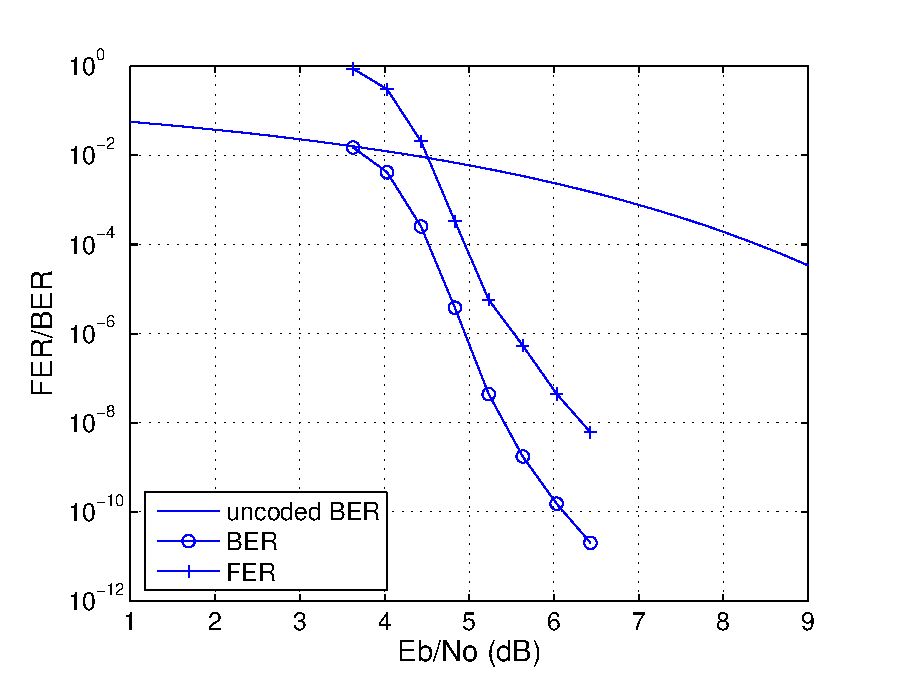
\includegraphics[keepaspectratio,width=3.0in,height=2.75in]{474_lara3.eps}
\caption{Experimental Results for $C_{47,4}$} \label{expif}
\end{figure}
%\newline \vspace{1.5in} \newline\vspace{0.0in}

%\vspace{1in}
%\vspace{4in}
%\vspace{-0.00in}\section{Conclusion and Future Work}\label{conc}
%The conclusion goes here.
\vspace{-0.00in}\section{Conclusion and Future Work}\label{conc}
%The conclusion goes here.



In this chapter we presented a detailed analysis of the dominant
configurations in the error-floor regime of high rate array-based
LDPC codes. We provided an explicit description of the minimal
(fully) absorbing sets and showed the non-existence of certain
candidate configurations. We also enumerated minimal (fully)
absorbing sets and showed how their number scales with the codeword
length. Experiments on an emulation platform were performed and were
found to be in agreement with the theoretical description of the
dominant errors.

%\chapter[Absorbing Sets of Tanner LDPC Codes]{Absorbing Sets Analysis of Tanner LDPC Codes}

\section{Tanner LDPC Code Construction}

\section{Theoretical Results}\label{theo1}

%\chapter{is}[is]

% avoiding spaces at the end of the author lines is not a problem with
% conference papers because we don't use \thanks or \IEEEmembership
% for over three affiliations, or if they all won't fit within the width
% of the page, use this alternative format:
%
%\author{\authorblockN{Michael Shell\authorrefmark{1},
%Homer Simpson\authorrefmark{2},
%James Kirk\authorrefmark{3},
%Montgomery Scott\authorrefmark{3} and
%Eldon Tyrell\authorrefmark{4}}
%\authorblockA{\authorrefmark{1}School of Electrical and Computer Engineering\\
%Georgia Institute of Technology,
%Atlanta, Georgia 30332--0250\\ Email: mshell@ece.gatech.edu}
%\authorblockA{\authorrefmark{2}Twentieth Century Fox, Springfield, USA\\
%Email: homer@thesimpsons.com}
%\authorblockA{\authorrefmark{3}Starfleet Academy, San Francisco, California 96678-2391\\
%Telephone: (800) 555--1212, Fax: (888) 555--1212}
%\authorblockA{\authorrefmark{4}Tyrell Inc., 123 Replicant Street, Los Angeles, California 90210--4321}}


% make the title area


\begin{abstract}
We present an importance sampling method for the evaluation of the low
frame error rate (FER) performance of LDPC codes under iterative
decoding.  It relies on a combinatorial characterization of absorbing
sets, which are the dominant cause of decoder failure in the low FER
region.  The biased density in the importance sampling scheme is a
mean-shifted version of the original Gaussian density, which is
suitably centered between a codeword and a dominant absorbing set.
This choice of biased density yields an unbiased estimator for the FER
with a variance lower by several orders of magnitude than the standard
Monte Carlo estimator.  Using this importance sampling scheme in
software, we obtain good agreement with the experimental results
obtained from a fast hardware emulator of the decoder.
\end{abstract}


\section{Introduction}

Low-density parity check (LDPC) codes are a class of binary linear
codes defined by very sparse factor graphs that yield excellent
error-correction performance when decoded iteratively using message
passing algorithms. Density evolution~\cite{richurbanke} accurately
characterizes their performance for large blocklengths.  However, for
moderate blocklengths---i.e., those on the order of hundreds to
thousands---the density evolution method can yield inaccurate results,
and thus current understanding of the finite length LDPC codes remains
incomplete.  In this moderate blocklength regime, many structured LDPC
codes exhibit an \emph{error floor}, corresponding to a significant
flattening in the curve that relates signal to noise ratio (SNR) to
the frame error rate (FER).  Consequently, despite the appeal of these
codes for many high data rate communications and data storage
applications, their wide-scale deployment has been hindered by
incomplete understanding of finite-length effects and error floors.
Better understanding of the performance of finite-length LDPC codes in
the low BER/FER regime has both theoretical as well as practical
implications. From a theoretical standpoint, it provides a deeper
understanding of the convergence of the message passing
algorithms. For practical storage and wireline applications, such
predictions provide a useful engineering tool in estimating performance
and designing LDPC codes.

Error-floor behavior can be attributed to the suboptimal nature of the
message passing algorithms used for decoding LDPC codes.  In early
work on error floors of LDPC codes, MacKay and Postol~\cite{mackay}
introduced the notion of a near-codeword.  Other related notions
include trapping sets~\cite{richardson},
pseudocodewords~\cite{Frey98}, and elementary trapping sets
\cite{milenkov}.  Based on our previous work~\cite{zhang06} using a
hardware emulator to explore the low FER region, we have isolated a
class of combinatorial structures that cause the decoder to fail by
converging to a non-codeword state. Due to their attractive nature, we
refer to these structures as \textit{absorbing sets}.  These
structures have a purely combinatorial definition in terms of the
parity check matrix defining the code, and can also be understood as a
particular type of near codeword~\cite{mackay} that is guaranteed to
be stable under a bit-flipping algorithm. For many LDPC codes, the
associated factor graphs contain absorbing sets which have strictly
fewer bits than the minimum codeword weight. As a result, the
performance of the decoding algorithm in the low FER region is
predominantly dictated by the number and the structure of minimal
absorbing sets, rather than the minimum distance
codewords~\cite{icc-theory}, as in the case of a maximum-likelihood
decoder.


In this paper, we investigate the low FER performance of a
$(2048,1723)$ Reed-Solomon based LDPC codes~\cite{rs-ldpc} as a
representative example of high-performance LDPC codes for which the
low FER region is dominated by non-codewords.  This particular RS-LDPC
code has been adopted in recent standards, and has a number of
desirable properties.  In this paper, we develop and demonstrate the
effectiveness of a fast simulation method, based on importance
sampling~\cite{Bucklew90}, for approximating the error probability.
As we discuss in more detail below, early work by
Richardson~\cite{richardson} demonstrated the effectiveness of a
two-stage approach, based on a combination of hardware emulation and
software-based simulation, for approximating the error probability.
Other work~\cite{ryan,ucla} has directly applied importance sampling
(IS), though limited to shorter blocklength codes and higher FERs than
those considered here.  For the RS-LDPC code, we first show how it is
possible to exactly enumerate all relevant classes of absorbing sets
that are dominant in the low FER regime.  We then exploit this
characterization of these absorbing sets to develop an efficient IS
method for evaluating the probability of error in the low FER regime.
The agreement with the experimental results obtained from the hardware
emulator demonstrates the power of the proposed technique, and
suggests that performance evaluation using the importance sampling
methods at even lower BER/FER levels yields reasonable
predictions. The computational advantage of the importance sampling
methods is demonstrated via their relative efficiencies--- namely, the
reduction in the sample variance of our IS-based estimators relative
to the sample variance of a naive Monte Carlo estimators, which
exceeds tens of millions.
%We also provide some new insight into the
%decoding regions around codewords and around absorbing sets, and we
%discuss how these regions change as a function of the decoder
%implementation.

The first paper (that we are aware of) that proposed a method for
predicting deep BER behavior of message-passing decoding algorithms is
by Richardson~\cite{richardson}.  This method consisted of two stages:
first identifying a class of (empirically defined) trapping sets via
hardware emulation, and then approximating its associated error
probability by simulating over a sequence of channel noises biased
towards the individual trapping set.  In contrast, our work is based
on graph substructures that have a combinatorial characterization in
terms of the Tanner graph, which we refer to as absorbing sets.  We
then approximate the error probability associated with a given
absorbing set by performing importance sampling at a single
mean-shifted distribution.  Our approach thus obviates the need to
empirically identify candidate trapping sets. While we may in theory
miss some error events through this approach, our simulation results
show sufficiently close agreement to our hardware emulations to argue
for the value of our approach.

 The remainder of the paper is organized as follows. In
Section~\ref{ldpcback}, we provide background on Reed-Solomon based
LDPC codes and absorbing sets.  Section~\ref{isback} describes the
Monte Carlo and importance sampling methods, and the specific IS-based
estimator used in this work.  Section~\ref{analysis} contains results
of the low FER rate performance using importance sampling. Lastly,
Section~\ref{conc} summarizes the results and proposes future
extensions.

%\vspace{1in}
\section{Background}

\label{ldpcback}

We begin with background on RS-LDPC codes, as well as on the notion
of absorbing sets.


\subsection{RS-LDPC codes}
Reed-Solomon based LDPC codes (RS-LDPC)~\cite{rs-ldpc} are regular,
structured LDPC codes, with the girth being at least 6.  The parity
check matrix of this code family can be viewed as consisting of a
two-dimensional array of permutation matrices of equal size. For the
row degree $\rho$ and the column degree $\gamma$, the construction is
based on stacking up $\gamma$ cosets of a one-dimensional subcode that
is itself determined by a weight $\rho$ codeword of a dimension 2
shortened Reed-Solomon code, followed by appropriately mapping these
symbols into binary row vectors. For the details of the construction,
please see Section III in the paper~\cite{rs-ldpc}.

The focus of this paper is the (2048,1723) RS-LDPC code, which has
column degree 6, row degree 32, and each component permutation
submatrix is of size 64 $\times$ 64.  This particular RS-LDPC has been
adopted in the IEEE 802.3an 10GBASE-T standard. The standard supports
10 Gb/s Ethernet over 100 meters of CAT-6a UTP (unshielded
twisted-pair) cable. The high frequency transmission is severely
impaired by insertion loss, cross talk, and interferences due to the
cable channel. These challenges present a stringent requirement on the
performance of the transceiver design. The $(2048,1723)$ RS-LDPC code
is selected specifically to provide sufficient coding gain to allow
for a bit error rate (BER) performance of $10^{-12}$ or
better~\cite{802standard}.  This code is designed to contain no cycles
of length 4 in the associated Tanner graph. It also features a
structured parity check matrix, amenable for a high throughput,
parallel decoder implementation. A lower bound on the the minimum
distance of this code is 8 by construction, though the actual minimum
distance is believed to be much higher. However, in our previous
hardware-based emulations~\cite{zhang06}, all error events recorded in
the low FER region were due to \emph{non-codeword} configurations.
More specifically, the decoder never converged to a non transmitted
codeword.  and all recorded errors were caused a single class of
combinatorial substructures.




\subsection{Absorbing sets}
As established in our previous experimental and theoretical
work~\cite{zhang06,icc-theory}, certain structures in the Tanner graph
associated with a parity check matrix of an LDPC code cause the
decoder to converge to a non-codeword state. We termed these
structures \emph{absorbing sets}, which are defined more formally as
follows:

\begin{figure}
%\vspace{0.1in}\hspace{0.2in}
%
\center
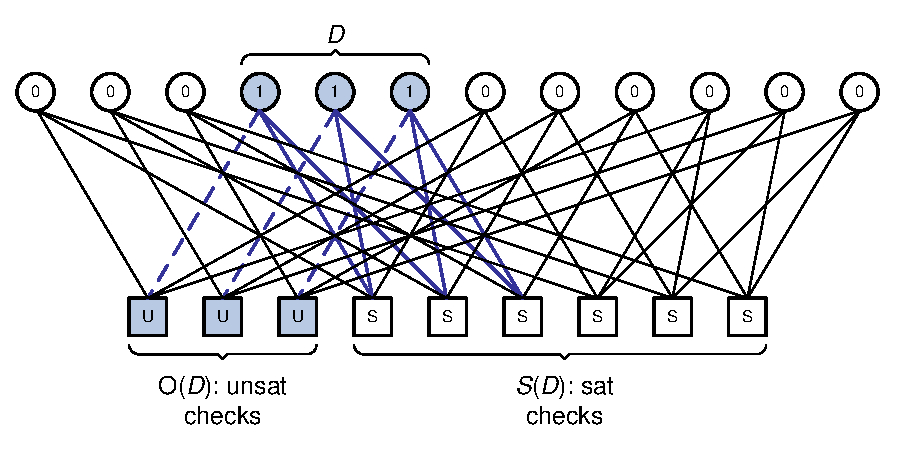
\includegraphics[width=3.2in,height=1.6in]{ITW07_33.eps}
%
\caption{An example of a (3,3) absorbing set.} \label{abs44}
\end{figure}

\vspace{0.0in}Let $G=(V,F,E)$ be a bipartite graph with the vertex
set $V \cup F$, where $V$ and $F$ are disjoint, and with the edge
set $E$, such that there exists an edge $e(i,j) \in E$ if and only
if $i\in V$ and $j\in F$.  One can associate a bipartite graph
$G_H=(V,F,E)$ with a parity check matrix $H$, such that the set $V$
corresponds to the columns of $H$, the set $F$ corresponds to the
rows of $H$, and $E=\{ e(i,j)| H(j,i)=1\}$. Such a graph $G_H$ is
commonly referred to as the Tanner graph of the parity check matrix
$H$ of a code. Elements of $V$ are called ``bit nodes'' and elements
of $F$ are called ``check nodes''. For the subset $D$ of $V$ we let
$N_D$ denote the set of check nodes neighboring the elements of $D$.

For a subset $D$ of $V$, let $\mathcal{E}(D)$ (resp.
$\mathcal{O}(D)$) be the set of neighboring vertices of $D$ in $F$
in the graph $G$ with even (resp. odd) degree with respect to $D$.
Given an integer pair $(a,b)$, an $(a,b)$ \emph{absorbing set} is
a subset $D$ of $V$ of size $a$, with $\mathcal{O}(D)$ of size $b$
and with the property that each element of $D$ has strictly fewer
neighbors in $\mathcal{O}(D)$ than in $F\backslash
\mathcal{O}(D)$. We say that an $(a,b)$ absorbing set $D$ is an
$(a,b)$ \emph{fully absorbing set}, if in addition, all bit nodes
in $V\backslash D$ have strictly more neighbors in $F\backslash
\mathcal{O}(D)$ than in $\mathcal{O}(D)$ \cite{icc-theory}.


Thus, absorbing sets correspond to a particular type of near-codeword,
distinguished by the additional requirement of each bit having
strictly more satisfied than unsatisfied checks.  An example of an
$(a,b)$ fully absorbing set with $a=b=3$ is given in Fig.~\ref{abs44}.
For the (2048, 1723) RS-LDPC code, the dominant (fully) absorbing sets
are (8,8) absorbing sets. An example of such a configuration is given
in Figure 2. The bits outside of the (fully) absorbing sets, though
omitted from the figure for clarity, are also assumed to have strictly
more satisfied than unsatisfied checks.


%\onecolumn
\begin{figure*}
\vspace{0.0in}\hspace{0.4in}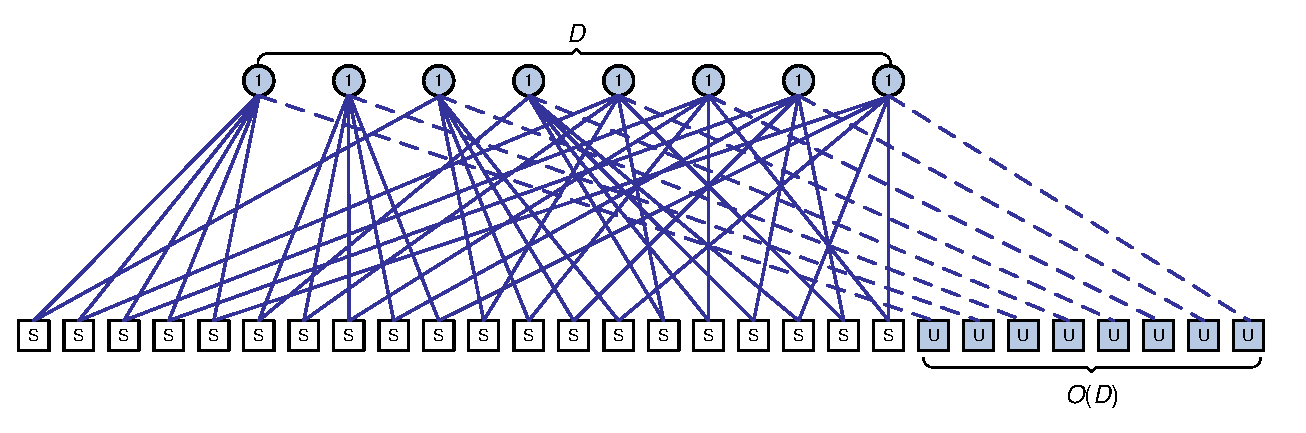
\includegraphics[width=5.4in,height=1.7in]{ITW07_88.eps}
\caption{An example of a (8,8) absorbing set for the $(2048,1723)$
RS-LDPC code.  Each of the $8$ bits in the set are connected to $4$
satisfied checks, and $1$ unsatisfied check.  } \label{abs88}
\end{figure*}
%\twocolumn





%\vspace{1in}


\vspace{0in}\section{Monte Carlo and Importance Sampling}
\label{isback}

Suitably designed LDPC codes of moderate blocklength yield excellent
performance when decoded with suboptimal iterative message-passing
algorithms.  The performance of an iteratively decoded LDPC code is
typically reported as the (empirical) probability of error for a
certain SNR value. For high SNR values, this empirical probability is
very small and thus a large number of trials needs to be executed in
order to estimate it reliably.

\subsection{Some intuition}

To provide some intuition for the typical number of samples required,
suppose that $p$ is the true probability of a decoding error at a
certain SNR level. A naive Monte Carlo simulation entails running the
decoder on $N$ independent channel realizations, and recording the
output of each trial $i= 1, \ldots, N$ with a Bernoulli indicator
variable
\begin{eqnarray*}
Z_i & \defn & \begin{cases} 1 & \mbox{if decoder fails on trial $i$} \\
                         0 & \mbox{otherwise.}
       \end{cases}
\end{eqnarray*}
It is assumed that the decoding error in the $i^\text{th}$ trial
occurs whenever the decoder does not converge to the transmitted
codeword in the fixed number of iterations.  These Bernoulli indicator
variables then yield the naive Monte Carlo estimate
\begin{eqnarray}
\label{EqnNaiveMC}
\hat{p}_{MC} & \defn & \frac{1}{N}\sum_{i=1}^N Z_i.
\end{eqnarray}
The Monte Carlo estimator is unbiased and has variance
$\var(\hat{p}_{MC})=\frac{1}{N}\left(\hat{p}_{MC}-\hat{p}_{MC}^2\right)$.

In order to characterize the quality of $\hat{p}_{MC}$ as an estimator
of $p$, we require that the relative error be small with high
probability, or equivalently that the tail probability
\begin{equation}
\label{EqnTail}
\mathbb{P} \left[ \left|\frac{\hat{p}_{MC}-p}{p}\right| > \epsilon
\right]
\end{equation}
should be small for an appropriate $\epsilon > 0$.  Some algebra
yields that
\begin{eqnarray*}
\mathbb{P} \left[ \left|\frac{\hat{p}_{MC}-p}{p}\right| > \epsilon
\right] & = & \mathbb{P} \left[ \frac{1}{N}\sum_{i=1}^N
\frac{Z_i-p}{\sqrt{p \,(1-p)}}> \epsilon \sqrt{\frac{p}{1-p}} \right].
\end{eqnarray*}
Since $Z_i$, $1 \leq i \leq N$ are i.i.d. Bernoulli random variables,
we may invoke the central limit theorem to approximate this
probability as the Gaussian tail function $\mathbb{P} [\left| Y
\right| > y]$, where $Y$ is a standard normal random variable and
\mbox{$y= \epsilon \sqrt{N \, p/(1-p)}$.}  As a concrete example, if
we require that for tolerance $\epsilon = 0.2$ the tail
probability~\eqref{EqnTail} be at most 0.05, corresponding to a 95\%
confidence interval, then we need $y \approx 2$, and thus $N \approx
100 (1-p)/p$. Consequently, in order to estimate a probability of
error that is around $10^{-8}$ up to relative error $\epsilon = 0.2$,
on the order of $10^{10}$ trials are needed. Such a requirement poses
a significant computational burden on available resources.


\begin{figure}\centering
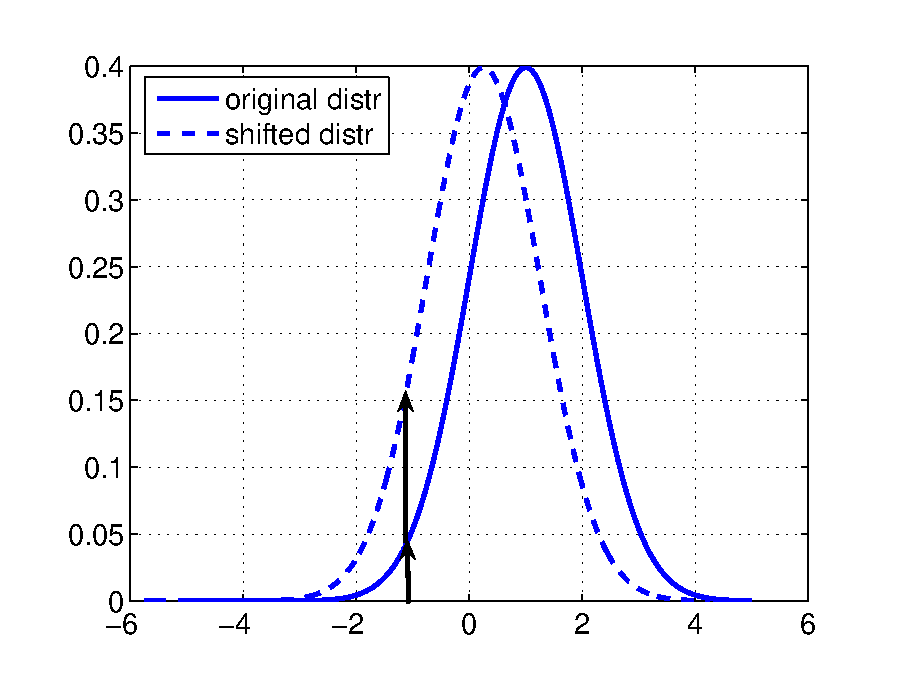
\includegraphics[width=2.4in,keepaspectratio]{itwfig3a_lara3.eps}
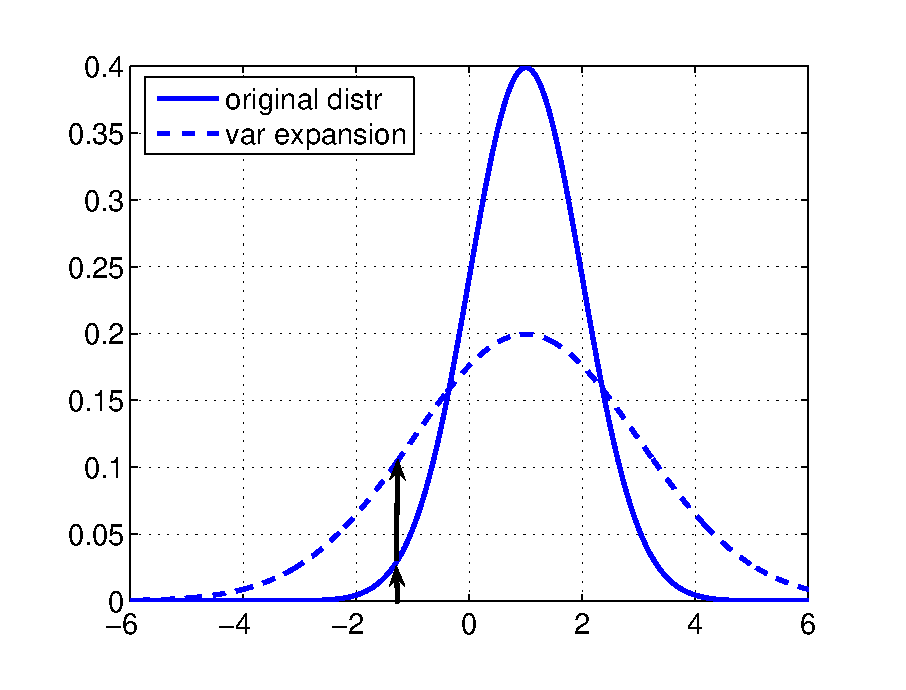
\includegraphics[width=2.4in,keepaspectratio]{itwfig3b_lara3.eps}
\caption{Examples of biasing densities (top: mean shift, bottom:
variance increase).} \label{bias}
\end{figure}

 The motivation underlying importance sampling is to appropriately
modify the original density such that the infrequent errors become
more likely. For a Gaussian density one may choose to shift the mean
or to scale the variance, as shown in the top and bottom panels of
Figure~\ref{bias} respectively.  In both cases the probability of the
event in the tail part (marked with an upward arrow in the Figures) of
the original distribution significantly increases.  The biasing
density should be chosen in such a way that the variance associated
with its estimator provides a substantial improvement over the
variance of a naive Monte Carlo estimator. Specifically, the ratio of
these two quantities indicates the reduction in the number of trials
needed to achieve the same confidence of the estimate of the
probability of error.

Supposing that one draws samples according to the biasing density
$f_{bias}$ instead of the original density, the importance sampling
estimator is computed as
\begin{eqnarray}
\label{EqnDefnIS}
\hat{p}_{IS} & = & \frac{1}{N}\sum_{i=1}^N Z_i w_i,
\end{eqnarray}
where the \emph{importance sampling weight} $w(x_i)
=f(x_i)/f_{bias}(x_i)$ reweights the contribution of the $i^{th}$
trial so that the estimator is unbiased ($\mathbb{E}[\hat{p}_{IS}] = p$).
Moreover, the IS variance is given by
\begin{eqnarray*}
\var(\hat{p}_{IS})=\frac{1}{N} \left( \frac{1}{N} \sum_{i=1}^N
\left(Z_i w_i \right)^2 -\hat{p}_{IS}^2 \right).
\end{eqnarray*}


\subsection{Error probabilities via mean-shifted importance sampling}

We propose to employ a biasing density $f_{bias}$ that makes the
decoder converge to an absorbing set more frequently.  As observed in
our previous work~\cite{zhang06} on the $(2048,1723)$ RS-LDPC code,
all errors in the low BER region are due to the absorbing sets of the
$(8,8)$ type.  We are concerned with the transmission over an AWGN
channel using BPSK modulation with mapping $0 \rightarrow +1$ and $1
\rightarrow -1$. Due to symmetry, we assume that the all-zeros
codeword is transmitted.  We choose $f_{bias}$ to be a mean-shifted
version of the original density $f$, which (assuming that the
all-zeroes codeword was transmitted) is a Gaussian density with mean
$[1 \; 1 \dots 1]$ and the variance $\sigma^2 I_{n \times n}$.  Since
$(8,8)$ absorbing sets dominate the low FER region, we set the mean
shift to be $\meanshift$ in the bits belonging to a particular $(8,8)$
absorbing set, and zero for the remaining bits.  As a result, the
importance sampling reweighting function $w(\cdot)$ takes the form
\begin{eqnarray}
\label{EqnDefnWeight} w(x; \meanshift, \sigma^2) & \defn &
\frac{e^{-\frac{1}{2 \sigma^2} \left[\sum_{j=1}^8 (x_{k_j}-1)^2
\right]}} {e^{-\frac{1}{2 \sigma^2} \left[\sum_{j=1}^8
(x_{k_j}-(1-\meanshift))^2\right]}}
\end{eqnarray}
where $k_1$ through $k_8$ are indices of the $8$ bits participating in
the $(8,8)$ absorbing set.

Importance sampling is most effective when the density is neither
underbiased nor overbiased, meaning that a reasonable choice for the
mean-shift $\meanshift$ is one which causes the decoder to return the
correct all-zeros codeword and to the targeted $(8,8)$ absorbing sets
with roughly equal probability.  In our work, we empirically
determined this point is chosen to be roughly $\meanshift = 1.2$. Note
that the contrast with maximum likelihood decoding where $\meanshift =
1$ defines the hyperplane separating decoding regions of two competing
codewords. Figure~\ref{tab1} lists the ratio of the decoding errors
over the total number of trials for different mean shifts. When the
total number of trials is fixed and relatively low, choosing the mean
shift value of $\meanshift = 0.8$ or less produces very infrequent
decoding errors. Likewise, for the the mean shift of $\meanshift =
1.6$ or higher, the decoder almost always makes an error, and coupled
with very low weighting terms $w(x)$ uniformly underestimates the
probability of error. For the middle region where $\meanshift$ is
between $1.0$ and $1.4$, the simulation results described in the next
section changed only negligibly with $\meanshift$.

%\vspace{0in} MISSING POINT 2: DISCUSSION OF MEAN SHIFT WRT
%VARIANCE.




\begin{figure}\center\begin{tabular}{|c|c|c|c|c|}
  \hline
  % after \\: \hline or \cline{col1-col2} \cline{col3-col4} ...
  Mean Shift & Ratio  \\
  \hline
  0.8 & 0.0134  \\
  1.0 & 0.1712  \\
  1.2 & 0.6292  \\
  1.6 & 0.9976  \\
  1.8 & 0.9999  \\
  \hline
\end{tabular}
\caption{Ratio of absorbing set errors and total number of trials
for the 6-bit decoder.}\label{tab1}
\end{figure}

%\begin{figure}
%\includegraphics[width=2.8in,height=1.6in]{Drawing1.ps}
%\caption{Illustration of the decoding region. } \label{decRegion}
%\end{figure}
%As illustrated in Figure~\ref{decRegion},
%The decoding region around a codeword is postulated to be larger than
%around a neighboring absorbing set.

Consider the set $S$ of the bit nodes in which the codeword and the
neighboring absorbing set disagree, and which participate in
unsatisfied checks in this absorbing set. Since the decoder aims to
have all checks satisfied, the values at these nodes in $S$ would have
to be strongly incorrect, i.e. close to the absorbing set in the
$n$-dimensional space, for their values not to be overcome by the
neighboring unsatisfied checks. The more of the unsatisfied checks
there are in the absorbing set, the smaller the decoding region of
that set is, since the values associated with the elements of $S$ need
to be reasonably close to the absorbing set values to resist the
messages sent from a large set of unsatisfied checks. Since for the
(8,8) set, there is one unsatisfied check per the bit node in the
absorbing set out of the total of 6 neighboring checks, the relative
size of the decoding region around this absorbing set is then somewhat
smaller than the one associated with the nearest codeword in the
direction of the coordinate which has value 0 for the codeword and 1
for the absorbing set.

While a variance-scaled Gaussian (see Fig.~\ref{bias}) may also be
considered as a candidate biasing density, choosing this density does
not lead to satisfactory results.  For smaller variance scalings, the
relative number of observed errors is quite small, so that a much
larger number of trials are required for estimates of accuracy
comparable to the mean-shifted estimator.
%in order to prevent extreme underestimation of the probability of
%error. Specifically, the increase in the number of trials relative to
%the mean-shifted biasing distribution for the same simulation gain is
%on the order of thousands, which defeats the purpose of quick
%simulation for estimation in the low FER regions.
As a concrete numerical illustration, we ran both the mean-shifted
importance sampler and and the variance-expanded importance sampler
for $N = 10^5$ trials each, grouped into $10$ sets of $10^4$ trials
each.  While the sample means for the mean-shifted importance sampler
were all within an order of magnitude, the sample means for the
variance-expansion importance sampler varied widely over 6 orders of
magnitude. In addition, the spread of the weighting terms $w(\cdot)$'s
for the variance-expanded importance sampler were exponentially larger
than for its mean-shifted counterpart.
%due in part to the more
%pronounced sensitivity of the weighting term to the multiplication of
%the argument in the exponential than to the translation of the
%argument.
On the other hand, if very high factor of variance expansion is used
so as to obtain a non-negligible fraction of decoding errors,
practical aspects of the decoder implementations can lead to numerical
instabilities.  In addition, for practical fixed-point
implementations, the input saturation applied before the iterative
decoding process further diminishes the usefulness of large variance
expansion.



\section{Experimental Results}
\label{analysis}

Since all $(8,8)$ absorbing sets have the same unlabelled
configuration, it suffices to choose a fixed representative of this
class of absorbing sets.  Accordingly, in the low FER regime, we may
approximate the probability of error as
\begin{eqnarray}
\label{EqnApprox}
\Prob[\mbox{error}; \sigma^2] & \approx & \; M \; \Prob(8,8; \sigma^2)
\end{eqnarray}
where $M$ is the total number of $(8,8)$ absorbing sets, and
$\Prob(8,8; \sigma^2)$ is the probability of decoding incorrectly
to any particular $(8,8)$ absorbing set with channel noise
$\sigma^2$. This approximation is reasonable, since the FPGA
results established that the $(8,8)$ absorbing sets are the
dominant cause of errors in the low FER regime.  In order to
evaluate this approximation, we estimated the absorbing set error
probability $\Prob(8,8; \sigma^2)$ by applying importance sampling
based on a mean shift $\meanshift = 1.2$ applied to only the $8$
bits that participated in this particular absorbing set.  For this
experiment, we choose bits with the index set $\{492, 497, 983,
988, 1572, 1596, 1880, 1904\}$ as the representative $(8,8)$
absorbing set.  As to the number of absorbing sets, for this
RS-LDPC code, we did an exact evaluation $M = 11,168$, by first
reducing the total starting number of choices to consider, namely
${2048 \choose 8}$, to a smaller set by imposing the constraints
the bit nodes in the absorbing set have to satisfy (e.g. a bit in
the absorbing set has to be a neighbor of a neighboring check of
another bit node in the absorbing set). We then counted the total
number of smaller configurations (whose number is on the order of
tens of thousands, a significant reduction from the starting count
which itself exceeds $10^{21}$) that need to be embedded within
one such absorbing set due to these relative constraints of the
nodes in the absorbing set. From these smaller configurations, and
by exploiting connectivity of the absorbing set nodes, the total
count of the (8,8) absorbing sets follows.





\subsection{Comparison for 6-bit decoder and for 9-bit decoders}


\vspace{0in} In this section we compare the importance sampling
methods previously described with the experimental results obtained
from the FPGA-based hardware emulator \cite{zhang06} for two different
quantization schemes. One scheme employs message quantization of 6
bits (4 for the integer and 2 for the fractional part), and the other
quantizes messages to 9 bits (4 for the integer and 5 for the
fractional parts). For both schemes we use the mean shift based
importance sampling applied to the bits in the representative
absorbing set to estimate the FER. The mean shift amount is 1.2 and a
total of 10000 trials are executed at each SNR point, in 0.1 dB
increments. We then approximate the overall FER according to the
expression~\eqref{EqnApprox}. The emulator curves and their importance
sampling counterparts are plotted in Figures~\ref{exp1} and
~\ref{exp2}.  Note the agreement in the slopes between the two sets of
curves.  We also compute the simulation gain $\gamma$ obtained by the
proposed approach relative to naive Monte Carlo, defined as~\cite{srini}
\begin{eqnarray*}
\gamma & \defn & \frac{\var(\hat{p}_{IS})}{\var(\hat{p}_{MC})}~.
\end{eqnarray*}
This gain corresponds to the reduction in the number of trials that
need to be performed using importance sampling in order to reach the
same confidence as the Monte Carlo simulation. The resulting
simulation gains are listed in Figures~\ref{table11} and
~\ref{table12} for the 6-bit and 9-bit decoders respectively, along
with the sample variance of the importance sampling estimator.
\begin{figure}
\vspace{0.0in}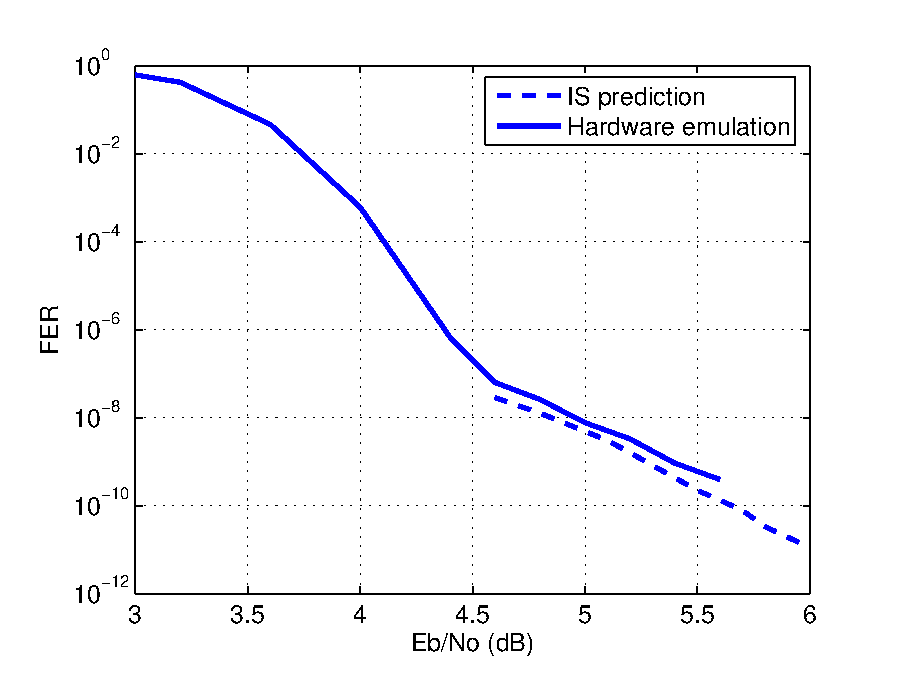
\includegraphics[width=2.8in,height=2.1in]{itwfig6_0619.eps}
\caption{Mean-shift IS bound and hardware results: 6-bit decoder.
}\label{exp1}
\end{figure}
\begin{figure}
\vspace{0.0in}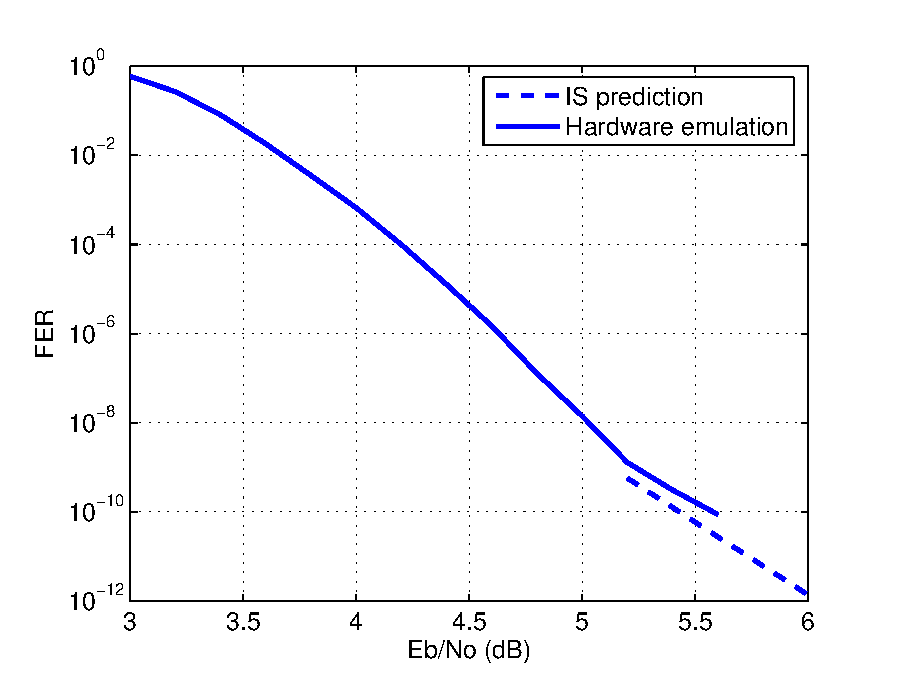
\includegraphics[width=2.8in,height=2.1in]{itwfig7_0619.eps}
\caption{Mean-shift IS bound and hardware results: 9-bit decoder.
}\label{exp2}
\end{figure}

\begin{figure}\center\begin{tabular}{|c|c|c|c|c|}
  \hline
  % after \\: \hline or \cline{col1-col2} \cline{col3-col4} ...
  SNR & Sample Variance & Simulation Gain \\
  \hline
  4.6 &  9.64E-25 & 4.6E6 \\
  4.8 &  2.29E-26 & 1.9E7 \\
  5.0 &  3.29E-27 & 2.77E7 \\
  5.2 &  1.18E-28 & 7.58E8 \\
  \hline
\end{tabular}
\caption{Simulation gains for the 6-bit decoder based on
mean-shift}\label{table11}
\end{figure}

\begin{figure}\center\begin{tabular}{|c|c|c|c|c|}
  \hline
  % after \\: \hline or \cline{col1-col2} \cline{col3-col4} ...
  SNR &  Sample Variance & Simulation Gain \\
  \hline
  5.2 & 3.7E-28 & 4.0E8 \\
  5.4 & 4.4E-29 & 6.72E8 \\
  5.6 & 4.07E-31 & 3.12E9 \\
  \hline
\end{tabular}
\caption{Simulation gains for the 9-bit decoder based on the
mean-shift.}\label{table12}
\end{figure}



 The above results demonstrate that even a
simple prediction is useful in estimating the performance of a
code in the low FER region. %For both quantization choices, the
%predicted importance sampling based curve provides an approximate
% bound on the probability of error that is within a factor of 10
%of the hardware based simulation results.
Moreover, since the
simulation gain increases with the increase in SNR, the
computational benefits of using the proposed importance sampling
based prediction increases with increased SNR/lower FER.

%\vspace{1in} MISSING POINT 3: DISCUSSION OF 6-BIT VS 9-BIT
%DECODING REGION

We now discuss the effects of the implementation choices on the
decoding region. As observed from Figures~\ref{exp1} and~\ref{exp2},
the error floor improves from a 6-bit decoder implementation to a
9-bit decoder implementation in hardware emulations. These additional
3 bits permit more quantization levels to better distinguish messages
during the message passing. Specifically, the soft messages in this
6-bit decoder suffer from more severe message saturations (clipping)
than in its 9-bit decoder counterpart. In the high-SNR error floor
regime, the clipping effect is more pronounced on strong ``good''
messages. These good messages do not have a strong enough
representation, thereby leading to an absorbing state where good
messages can be overcome by the sheer number of bad messages. As a
result, the decoder is more easily pulled into the absorbing state
under the 6-bit quantization than under the 9-bit quantization. This
effect can be also seen from the observation that under the same mean
shift, the relative number of errors for the 6-bit quantization scheme
is uniformly higher than for the 9-bit scheme, as seen by comparing
Tables~\ref{tab1} and~\ref{tab4}. (Note that both simulations are
based on $N = 10^4$ trials at SNR $5.4$ dB.)
% This intuition is also confirmed by hardware emulations of a 6-bit
%decoder, in which we observed a stronger tendency towards the
%absorbing state compared to a 9-bit
%decoder. %MISSING PT 3: CONNECTION TO THE DECODING REGION
%We thus conjecture that with the help of a relatively small mean
%shift, this tendency can be accentuated, causing absorbing-set
%errors. Accordingly, the convergence region of an absorbing set in
%a 6-bit decoder is larger than the convergence region of a 9-bit
%decoder.

\begin{figure}\center\begin{tabular}{|c|c|c|c|c|}
  \hline
  % after \\: \hline or \cline{col1-col2} \cline{col3-col4} ...
  Mean Shift & Ratio  \\
  \hline
  0.8 &   0.0060\\
  1.0 &   0.1002\\
  1.2 &   0.4944\\
  1.6 &   0.9890\\
  \hline
\end{tabular}
\caption{Ratio of absorbing set errors and total number of trials
for the 9-bit decoder.}\label{tab4}
\end{figure}
\section{Concluding Remarks}\label{conc}

LDPC codes have recently generated a lot of interest due to their
excellent performance. While the infinite blocklength regime is better
understood, less is known about the performance of LDPC codes for
finite blocklengths. Since the performance of finite blocklength LDPC
codes for low FER rates cannot be estimated reasonably fast using
software based Monte Carlo simulations, along with the lack of
finite-length theoretical analysis, the deployment of LDPC has so far
been somewhat limited.

In this paper, we presented a technique for estimating probability of
decoding error of LDPC codes in the low FER/BER regime. The proposed
method utilizes importance sampling to quickly produce the estimate of
the performance. With appropriately biased densities, the runtime
speed-up is on the order of millions. In conjunction with the
description and count of dominant absorbing errors, the proposed
technique provides accurate estimates of the probability of error in
the low FER regime. Results obtained on a hardware emulator are
consistent with the proposed technique, and thus suggest the promise
of using the proposed approach at even lower FER/BER levels.

As to future directions, we plan to extend the proposed methodology to
other LDPC codes with different absorbing set configurations and their
distributions as well as to investigate how the decoding regions
associated with the codewords and the absorbing sets scale as a
function of the decoder choices, specifically including the min-sum
algorithm as a less complex version of the message passing decoding.

\chapter[Conclusion and Future Extensions]{Conclusion and Future Extensions}
\label{ch:conclusion}

MapReduce has proven to be a popular model for large-scale parallel programming. Our Hadoop Online Prototype extends the applicability of the model to pipelining behaviors, while preserving the simple programming model and fault tolerance of a full-featured MapReduce framework.  This provides significant new functionality, including ``early returns'' on long-running jobs via online aggregation, and continuous queries over streaming data.  We also demonstrate benefits for batch processing:  by pipelining both within and across jobs, HOP can 
%achieve increased parallelism, improved system utilization, and 
reduce the time to job completion. 

In considering future work, scheduling is a topic that arises immediately.
Stock Hadoop already has many degrees of freedom in scheduling batch tasks across machines and time, and the introduction of pipelining in HOP only increases this design space.  First, pipeline parallelism is a new option for improving performance of MapReduce jobs, but needs to be integrated intelligently with both intra-task partition parallelism and speculative redundant execution for ``straggler'' handling.
%But given a fixed budget of task slots the cluster can run, pipeline depth has to be traded off against the number of concurrent partitions of a single dataflow stage (a single map or reduce).  We hope to expose these tradeoffs better via a closer analysis of the burstiness of resource consumption in stock Hadoop, and the resulting opportunity to smooth those bursts with pipelined parallelism.  
Second, the ability to schedule deep pipelines with direct
communication between reduces and maps (bypassing the distributed file
system) opens up new opportunities and challenges in carefully co-locating tasks from different jobs, to avoid communication when possible.  
%Finally, pipelining has tradeoffs with the use of map-side combiners.  As noted in Section~\ref{ch:hop:sec:pipelining}, for jobs that generate a small number of distinct reduce keys (e.g., genders), eager pipelining defeats the data reduction opportunities available with a blocking map-side combiner. For jobs with many reduce keys, or with no combiner available (e.g. Sort), aggressive pipelining may be a wise choice, to enable pipelined parallelism.  Since the number of distinct reduce keys is not typically known in advance, the choice of batch sizes for pipelining should be chosen in a dynamic fashion based on introspection during processing.  This introspection could be node-local, or could be a global decision fed by a continuous monitoring query of the sort illustrated in Section~\ref{ch:hop:sec:continuous}.  

Olston and colleagues have noted that MapReduce systems---unlike traditional databases---employ ``model-light'' optimization approaches that gather and react to performance information during runtime~\cite{olston-usenix08}.  The continuous query facilities of HOP enable powerful introspective programming interfaces for this: a full-featured MapReduce interface can be used to script performance monitoring tasks that gather system-wide information in near-real-time, enabling tight feedback loops for scheduling and dataflow optimization.  This is a topic we plan to explore further, including opportunistic methods to do monitoring work with minimal interference to outstanding jobs, as well as dynamic approaches to continuous optimization in the spirit of earlier work like Eddies~\cite{eddies} and FLuX~\cite{flux-lb}.

% Inter-job pipelining brings up some interesting opportunities for optimization as well. First, if we have a chain of two jobs, we can have the
% first job write its output to the local disk instead of going to HDFS. This
% saves the HDFS overhead at the expense of the risk of local disk failure.
% Since the intermediate data is relatively ephemeral, the window of risk may be tolerable in many cases. Second, we want to try scheduling maps of second job at nodes where reduces of the first job are running. This way data pipelining will be done locally and will not have to go through the network.

% Online aggregation changes some of the scheduling criteria in cases where there are not enough slots systemwide for all of a job's tasks.  Map and reduce tasks affect an online aggregation job differently: leaving map tasks unscheduled is akin to sampling the input file, whereas leaving reduce tasks unscheduled is akin to missing certain output keys -- some of which could be from groups with many inputs.  This favors reducers over mappers, at least during early stages of processing.  

% In order to improve early results of pipelined flows (e.g., for online aggregation), it is often desirable to prioritize ``interesting'' data in the pipeline, both at the mapper and reducer.  Online reordering of data streams has been studied in the centralized setting~\cite{juggle}, but it is unclear how to expose it in the MapReduce programming framework, with multiple nodes running in parallel -- especially if the data in the input file is not well randomized.  

%Continuous queries over streams raise many specific opportunities for optimizations, including sharing of work across queries on the same streams, and minimizing the work done per query depending on windowing and aggregate function semantics.  Many of these issues were previously considered for tightly controlled declarative languages on single machines~\cite{stream,tcq-cidr}, or for wide-area pipelined dataflows~\cite{borealis,sbon}, and would need to be rethought in the context of a programmable MapReduce framework for clusters.
 % many of which have been well-studied in the literature and should port naturally to a MapReduce setting, as demonstrated in initial work on the topic~\cite{logoyocum08}.  One key issue in the literature is the sharing of work across multiple queries on the same stream~\cite{precisionsharing,huebsch}; but prior work does not necessarily map well to a MapReduce framework, and the issue deserves more investigation.  
%Introspective system monitoring is a good driving application here, since it provides a well-motivated workload that developers of the system are well-motivated to study in depth.  

As a more long-term agenda, we want to explore using MapReduce-style programming for even more interactive applications.  As a first step, we hope to revisit interactive data processing in the spirit of the CONTROL work~\cite{ieeecontrol}, with an eye toward improved scalability via parallelism.  More aggressively, we are considering the idea of bridging the gap between MapReduce dataflow programming and lightweight event-flow programming models like SEDA~\cite{seda}.  Our HOP implementation's roots in Hadoop make it unlikely to compete with something like SEDA in terms of raw performance. However, it would be interesting to translate ideas across these two traditionally separate programming models, perhaps with an eye toward building a new and more general-purpose framework for programming in architectures like cloud computing and many-core.



% ===============================
% Part III: Back Matters
%           - bibliography
%           - appendix
%           - index
% ===============================

%\ssp
%\bibliographystyle{ieeetr}
\bibliography{refs}
 %\addcontentsline{toc}{section}{References}
\begin{thebibliography}{10}
\bibitem{aji}
S. Aji and R. McEliece, ``The generalized distributive law",
\emph{IEEE Transactions on Information Theory} vol.\ 46(2),
pp.~325--43, March 2000.

\bibitem{ammer}
M. J. Ammer, \emph{Low Power Synchronization for Wireless
Communication}, PhD Thesis, EECS Dept., UC Berkeley, 2004.

\bibitem{apostol} T. M. Apostol, ``\emph{Introduction to Analytic Number
Theory}'', Springer-Verlag, NY, 1976.


\bibitem{iterativetr:04}
J.~Barry, A.~Kavcic, S.~McLaughlin, A.~Nayak, and W.~Zeng,
\newblock {``Iterative timing recovery"},
\newblock {\em IEEE Signal Processing Magazine}, 21:89--102, January 2004.

\bibitem{bose:67}
R.~C.~Bose and J.~G. Caldwell
\newblock {``Synchronizable error-correcting codes"},
\newblock {\em Information and Control}, 10:616--630, 1967.

\bibitem{bours:94}
P. A. H. Bours, ``Construction of fixed-length insertion/deletion
correcting runlength-limited code", \emph{IEEE Transactions on
Information Theory}, vol.\ 40(6), pp.~1841--1856, Nov. 1994.


\bibitem{calabi:69}
L.~Calabi and W.~E. Hartnett,
\newblock {``A family of codes for the correction of substitution and
  synchronization errors"},
\newblock {\em IEEE Trans. Inform. Theory}, 15(1):102--106, January 1969.

\bibitem{cmnv:03}
G.~Chen, M.~Mitzenmacher, C.~Ng, and N.~Varnica,
\newblock {``Concatenated codes for deletion channels"},
\newblock In {\em {Proceedings of the IEEE International Symposium on
  Information Theory}}, Yokohama, Japan, 2003.


\bibitem{chertkov} M. Chertkov and V.Y. Chernyak, ``Loop calculus
helps to improve belief propagation and linear programming decodings
of low-density-parity-check codes, " Proceedings of the \emph{44th
Annual Allerton Conf. on Communications, Control and Computing},
Monticello, IL, USA, Sep. 27-29, 2006.

\bibitem{chung}
S.-Y. Chung, G. D. J. Forney, T. Richardson, and R. Urbanke ``On the
design of low-density parity-check codes within 0.0045 dB of the
Shannon limit", \emph{IEEE Communications Letters}, vol. 5, no. 2.
pp.58--60, 2001.

\bibitem{cf:03}
W.~A. Clarke and H.~C. Ferreira,
\newblock {``A new linear, quasicyclic multiple insertion/deletion correcting
  code"},
\newblock In {\em {2003 IEEE Pacific Rim Conference on Communications Computers
  and Signal Processing}}, 2003.

\bibitem{clarke:93}
W.~A. Clarke, A.~S.~J. Helberg, and H.~C. Ferreira,
\newblock {``Constrained codes for the correction of synchronization and
  additive errors"},
\newblock In {\em {Proceedings of the 1993 IEEE South African Symposium on
  Communications and Signal Processing. COMSIG}}, New York, NY, USA, 1993.

\bibitem{dmackay:01}
M.~C. Davey and D.~J.~C. MacKay,
\newblock {``Reliable communication over channels with insertions, deletions and
  substitutions"},
\newblock {\em IEEE Trans. Inform. Theory}, 47(2):687--698, Feb. 2001.


\bibitem{di_stop} C. Di, D. Proietti, T. Richardson, E. Telatar,
and R. Urbanke, "Finite length analysis of low-density parity-check
codes on the binary erasure channel," \emph{IEEE Transactions on
Information Theory}, vol.\ (48), pp.~1570--1579, 2002.


\bibitem{isit06} L. Dolecek and V. Anantharam, ``A synchonization
technique for array-based LDPC codes'', \emph{International
Symposium on Information Theory}, Seattle, WA, July 9-13, 2006.


\bibitem{dRMSupTech:06}
L.~Dolecek,
\newblock {``On Structural Properties of Reed-Muller RM($1$,$m$) Codes and Their
  Use in Channels with Synchronization Errors"},
\newblock Technical report, EECS Dept., UC Berkeley, April 2006.
\newblock {Available online at http://www.eecs.berkeley.edu/Pubs/TechRpts/2006/EECS-2006-43.pdf
}

\bibitem{itw:07}
L. Dolecek, Z. Zhang, M. Wainwright, V. Anantharam, and B. Nikolic,
``Evaluation of the low frame error rate performance of LDPC codes
using importance sampling," \emph{Information Theory Workshop}, Lake
Tahoe, CA, Sept. 2007.
%\bibitem{daArrayTech:06}
%L.~Dolecek and V.~Anantharam,
%\newblock {``On Array-Based LDPC Codes in Channels With Varying Sampling
%Rate"},
%\newblock Technical report, EECS Dept., UC Berkeley, Jan. 2006.
%\newblock {Available online at
%http://www.eecs.berkeley.edu/Pubs/TechRpts/2006/EECS-2006-7.pdf }
\bibitem{ibm:02} % linear time encoding    dsl app
E. Eleftheriou and S. \"{O}l\c{c}er, "Low density parity check codes
for digital subscriber lines", \emph{Proc. of the IEEE Int. Conf. on
Commun.}, New York, NY, 2002, pp.~1752--1757.

\bibitem{fan}
J. L. Fan, ``Array-codes as low-density parity-check codes,''
\emph{Second Int. Symp. on Turbo Codes}, Brest, France, pp.~543--46,
Sept. 2000.

\bibitem{wainwrig}
J. Feldman, M. J. Wainwright and D. R. Karger, ``Using linear
programming to decode binary linear codes'', \emph{IEEE Transactions
on Information Theory}, vol.\ (51), pp.~954--972.


\bibitem{ferr:97}
H. C. Ferreira, W. A. Clarke, A. S. J. Helberg, K. A. S.
Abdel-Gaffar and A. J. Han Vinck, ``Insertion/deletion correction
with spectral nulls", \emph{IEEE Transactions on Information
Theory}, vol.\ 43(2), pp.~722--732, March 1997.

\bibitem{forney}
G. D. Forney, ``Codes on graphs: normal realizations'', \emph{IEEE
Trans. Inform. Theory}, vol.\ (47), pp.~520--548, Feb. 2001.

\bibitem{gall}
R. Gallager, \emph{Low Density Parity Check Codes}, MIT Press, 1964.

\bibitem{GR61}
E. N. Gilbert and J. Riordan, ``Symmetry types of periodic
sequences", \emph{Illinois Journal of Mathematics}, Vol. 5, pp.
657--665, 1961.


\bibitem{ferr:02}
A. S. J. Helberg and H. C. Ferreira, ``On multiple
insertion/deletion correcting codes", \emph{IEEE Transactions on
Information Theory} vol.\ 48(1), pp.~305--308, Jan. 2002.

\bibitem{gallager}
R. G. Gallager, \emph{Low Density Parity Check Codes}, Monograph,
M.I.T. Press, 1963.

\bibitem{huavan:49}
L. K. Hua and H. S. Vandiver, ``Characters over certain types of
rings with applications to the theory of equations in a finite
field'', \emph{Proc. Nat. Acad. Sci. USA}, vol. 35, pp.~481-487,
1949.

\bibitem{kashyap:03}
N. Kashyap and A. Vardy, ``Stopping sets in codes from designs,"
\emph{International Symposium on Information Theory}, pp.~122,
Yokohama, Japan, July, 2003.

\bibitem{klove:95}
T.~Kl{\o}ve,
\newblock {``Codes correcting a single insertion/deletion of a zero or a single
  peak-shift"},
\newblock {\em IEEE Trans. Inform. Theory}, 41(1):279--283, January 1995.


\bibitem{vontobel}
R. Koetter and P. Vontobel, ``Graph covers and iterative decoding of
finite-length codes," Procedings of the \emph{Third International
Symposium on Turbo Codes and Related Topics}, Brest, France,
pp.~75-82, Sept. 2003.

\bibitem{kbek:04}
P.~Kovintavewat, J.~R. Barry, M.~F. Erden, and E.~Kurtas,
\newblock {``Per-survivor timing recovery for uncoded partial response
  channels"},
\newblock In {\em {Proceedings of the IEEE International Conference on
  Communications}}, 2004.

\bibitem{foss01}
Y. Kou, S. Lin, and M. P. C. Fossorier, ``Low-density parity-check
codes based on finite geometries: arediscovery and new results''
\emph{IEEE Transactions on Information Theory}, vol. 47, no. 7,  pp.
2711 - 2736, Nov. 2001.


\bibitem{milenkov} S. Laendner and O. Milenkovic, ``Algorithmic and
combinatorial analysis of trapping sets in structured LDPC codes, ''
in \emph{Wireless Comm}, Hawaii, USA, 2005.

\bibitem{lev:66a}
V. I. Levenshtein, "Binary codes capable of correcting spurious
insertions and deletions of ones", \emph{Problems of Information
Transmission}, vol.\ 1(1),pp.~8--17, Jan. 1965.

\bibitem{lev:66}
V. I. Levenshtein, "Binary codes capable of correcting deletions,
insertions and reversals", \emph{Sov. Phys.-Dokl.}, vol.\ 10(8),
pp.~707--710, Feb. 1966.


\bibitem{lev:92}
V.~I. Levenshtein,
\newblock {``On perfect codes in deletion and insertion metric"},
\newblock {\em Discrete Math. Appl.}, 2(3):241--258, 1992.

\bibitem{lincostello}
S. Lin and D. Costello, \emph{Error Control Coding}, Second Edition,
Prentice Hall, 2004.

\bibitem{liu:02}
J.~Liu, H.~Song, and B.V.K.V. Kumar,
\newblock {``Symbol timing recovery for low-SNR partial response recording
  channels"},
\newblock In {\em {GLOBECOM'02 - IEEE Global Telecommunications Conference}},
  2002.
\bibitem{mackay96}
D. MacKay and R. Neal, ``Near Shannon limit performance of low
density parity check codes'', \emph{Electronic Letters}, vol. 32,
no. 18, pp. 1645--46, August 1996.

\bibitem{mackay} D. MacKay and M. Postol, ``Weaknesses of Margulis
and Ramanujan-Margulis low-density parity-check codes,"
\emph{Electronic Notes in Theoretical Computer Science}, vol. 74,
2003.

\bibitem{mws:77}
F.~J. MacWilliams and N.~J.~A. Sloane,
\newblock {\em {``The Theory Of Error Correcting Codes"}},
\newblock North Holland Publishing Company, Amsterdam, Holland, 1977.


\bibitem{mittel:02}
T. Mittelholzer, ``Efficient encoding and minimum distance bounds of
Reed-Solomon-type array codes,'' \emph{International Symposium on
Information Theory}, Lausanne, Switzerland, July 2002, p. 282.

\bibitem{mcla:02}
A.~R. Nayak, J.~Barry, and S.~W. McLaughlin,
\newblock {``Joint timing recovery and turbo equalization for coded partial
  response channels"},
\newblock {\em IEEE Trans. On Magnetics}, 38(5):2295--97, Sept. 2002.

\bibitem{orlitsky:93}
A. Orlitsky, Interactive communication of balanced distributions and
of correlated files, \emph{SIAM Journal on Discrete Mathematics},
vol.\ 6(4), pp.~548--564, Nov. 1993.

\bibitem{orlitsky:05}
A. Orlitsky, K. Viswanathan, and J. Zhang, ``Stopping set
distribution of LDPC code ensambles," \emph{IEEE Transactions on
Information Theory} vol.\ 51(3), pp.~929--53, March 2005.

\bibitem{peterson}
W. W. Peterson and  E. J. Weldon, \emph{Error Correcting Codes}, MIT
Press 1972.

\bibitem{rrumely}
O. Ramare and R. Rumely, ``Primes in arithmetic progressions",
\emph{Mathematics of Computation}, vol.\ 65, No. 213, pp.~397 --425,
Jan. 1996.

\bibitem{richardson}
T. Richardson, ``Error floors of LDPC codes", Proceedings of the
Allerton Conference on Communications, Control and Computing, 2003.

\bibitem{richurbanke}
T. Richardson and R. Urbanke, ``The capacity of low-density
parity-check codes under message-passing decoding'', \emph{IEEE
Transactions on Information Theory}", Vol.~47. no.~2, pp. 599--618,
Feb. 2001.

\bibitem{rosser:62}
J. B. Rosser and L. Schoenfeld, ``Approximate formulas for some
functions of prime numbers", \emph{Illinois Jour. Math.}, vol.\
6(1), pp.~64--94, March 1962.

\bibitem{sloane:00} N. J. A. Sloane, "On single deletion
correcting codes", 2000. Available at
http://www.research.att.com/\~{ }njas/doc/dijen.pdf

\bibitem{sopro}
I. Soprounov, ``A short proof of the prime number theorem for
arithmetic progressions", available online at
http://www.math.umass.edu/~isoprou/pdf/primes.pdf

\bibitem{stiffler:65}
J.~.J.~Stiffler,
\newblock {``Comma free error correcting codes"},
\newblock {\em IEEE Trans. Inform. Theory}, 11:107--112, 1965.

\bibitem{ferr:03}
T. G. Swart and H.C. Ferreira, "A note on double
insertion/deletion correcting codes", \emph{IEEE Transactions on
Information Theory} vol.\ 49(1), pp.~269--273, Jan. 2003.

\bibitem{ten:84}
G.~Tenengolts,
\newblock {``Nonbinary codes correcting single deletion or
insertion"},
\newblock {\em IEEE Trans. Inform. Theory}, 30:766--769, Sept. 1984.

\bibitem{ullman:66}
J.~D. Ullman.
\newblock {``Near optimal single synchronization error correcting
code"},
\newblock {\em IEEE Trans. Inform. Theory}, 12:418--424, 1966.

\bibitem{vt:65}
R. R. Varshamov and G.M. Tenengolts, ``Codes which correct single
asymmetric errors,'' \emph{Avtomatika i Telemehkanika}, vol.\ 26,
no. 2, pp.~288--292, 1965.

\bibitem{vasic:05} % book for mr apps
B. Vasic and E. Kurtas, "Coding and Signal Processing for Magnetic
Recording Systems", CRC press, 2005.

\bibitem{weil:49}
A. Weil, ''Numbers of solutions of equations in finite fields", in
\emph{Bull. Amer. Math. Soc}, vol. 50, pp.~497--508, 1949.

\bibitem{wicker}
S.B. Wicker, \emph{Error Control Systems for Digital Communication
and Storage}, Prentice Hall, 1995.

 \bibitem{helles}
K. Yang and T. Helleseth, ``On the minimum distance of array codes
as LDPC codes", \emph{IEEE Trans. Inform. Theory}, vol.\ 49(12),
pp.~3268--3271, Dec. 2003.

\bibitem{zhangkavcic:03}
W.~Zhang and A.~Kavcic,
\newblock {``Optimal soft output detector for channels with intersymbol interference and timing
errors"},
\newblock {\em IEEE Trans. Magnetics}, 49(5):2555--557, Sept. 2003.


\bibitem{zhang06}
Z. Zhang, L. Dolecek, B. Nikolic, V. Anantharam and M. Wainwright,
``Investigation of error floors of structured low-density
parity-check codes via hardware simulation", in \emph{Proc.
GLOBECOM 2006}, San Francisco, CA, Oct.-Nov. 2006.


\bibitem{ICCquant}
Z. Zhang, L. Dolecek, M. J. Wainwright, V. Anantharam, B. Nikolic,
``Quantization effects of low-density parity-check decoders,'' in
Proceedings of \emph{IEEE International Conference on
Communications}, Glasgow UK, June 2007.

\bibitem{dvbstandard}
Digital Video Broadcasting Project, available at http://www.dvb.org

\bibitem{802standard}
IEEE Standard 802.3an-2006, Sept. 2006 Available at
http://ieeexplore.ieee.org/servlet/opac?punumber=4039890

\bibitem{cluster} \emph{Performance evaluation of low latency LDPC code}, 802.3an Standards
Meeting, Sept. 2004. Available online at
http://www.ieee802.org/3/an/public/sep04/seki10904.pdf


\end{thebibliography}

%\include{append}

\end{document}
